%%%%%%%%%%%%%%%%%%%%%%%%%%%%%%%%%%%%%%%%%%%%%%%%%%%%%%%%%%%%%%%%%%%%%%
% Lớp 11 | Quan hệ vuông góc trong không gian | Góc giữa đường thẳng và mặt phẳng. Góc nhị diện
% Dạng 1H8?6-1: Góc giữa đường thẳng và mặt phẳng
% Số câu: 156  (sinh tự động bởi tach_cau.py; từ nay thầy sửa trực tiếp file này)
%%%%%%%%%%%%%%%%%%%%%%%%%%%%%%%%%%%%%%%%%%%%%%%%%%%%%%%%%%%%%%%%%%%%%%

%%%%%%%%%%%%%%%% TRẮC NGHIỆM 4 PHƯƠNG ÁN %%%%%%%%%%%%%%%%

% nguồn: Ok_Toan11_TracNghiem_Lan2
\begin{ex}%[1H8N6-1]%[ma:5e4e20b0]
	\immini[thm]{ 
	Cho hình chóp $S.ABC$ có đáy $ABC$ là tam giác vuông cân tại $A$, $AB=a$, $SB \perp (ABC)$, $SB=a\sqrt{2}$. Gọi  góc giữa $SC$ và $(SAB)$ là $\alpha$. Tính $\tan\alpha$.
	\choice 
		{\True $\tan\alpha=\dfrac{1}{\sqrt{3}}$} 
		 {$\tan\alpha=\dfrac{1}{2}$}
		 {$\tan\alpha=\dfrac{\sqrt{3}}{2}$}
		{$\tan\alpha=\sqrt{3}$} 
		 }{
		\begin{tikzpicture}[>=stealth,line join=round,line cap=round,font=\footnotesize,scale=1]
				\tikzset{ 
					pics/chopTamGiac/.style  n args={4}{
					code={ 
				 \tikzset{declare function={a=4; b=3; h=3; goc=-20;}}
				\path 
					(0,0) coordinate (#1)+(0:a) coordinate (#3)+ 
					(goc:b)  coordinate (#2)
					 ($(#1)+(90:h)$) coordinate (#4);
				\foreach  \pointo/\pointt in {#4/#1,#1/#2,#2/#3,#3/#4,#4/#2}{
					 \draw[fill=black](\pointo)--(\pointt);
				 }
				\foreach  \pointo/\pointt in {#1/#3}{
					 \draw[fill=black,dashed](\pointo)--(\pointt);
				 }
				 }
					}} 
				 \path
					(0,0) coordinate (a)  pic{chopTamGiac={B}{A}{C}{S}};
				\foreach \point/\goc in  {S/90,B/210,A/-90,C/-10}{
					\draw[fill=black](\point) circle (.8pt)+(\goc:2mm)  node[scale=.8]{$\point$};
				} 
			\end{tikzpicture}
		 }
	\loigiai{ 
		Ta có $\heva{& AC \perp AB \text{  (do } \triangle ABC \text{ vuông tại } A) \\ & AC \perp SB \text{ (do } SB \perp (ABC)).}$ \\
		Suy  ra $AC \perp (SAB)$.\\
		Do đó, hình chiếu  của $SC$ lên mặt phẳng $(SAB)$ là $SA$.\\
		Suy ra $\alpha = (SC,  (SAB)) = (SC, SA) = \widehat{ASC}$.\\
		Tam giác  $ABC$ vuông cân tại $A$ nên $AC=AB=a$.\\
		Tam giác $SAB$ vuông tại $B$ (do $SB \perp (ABC)$), áp  dụng định lí Pythagore ta có
		\[SA=\sqrt{SB^2+AB^2}=\sqrt{\left(a\sqrt{2}\right)^2+a^2}=\sqrt{2a^2+a^2}=a\sqrt{3}.\] 
		Tam giác $SAC$ vuông tại $A$ (do $AC \perp  (SAB)$), ta có
		\[\tan\alpha=\tan\widehat{ASC}=\dfrac{AC}{SA}=\dfrac{a}{a\sqrt{3}}=\dfrac{1}{\sqrt{3}}.\] 
	} 
\end{ex}

% nguồn: Ok_Toan11_TracNghiem_Lan2
\begin{ex}%[1H8N6-1]%[ma:39068512]
	\immini[thm]{ 
	Cho hình chóp $S.ABCD$ có đáy $ABCD$ là  hình chữ nhật và $SA \perp (ABCD)$ như hình vẽ bên. Góc giữa đường thẳng $SD$ và mặt phẳng $(ABCD)$ là
	\choice 
		{$\widehat{ASD}$} 
		{$\widehat{DAS}$} 
		{\True  $\widehat{SDA}$}
		{$\widehat{SDC}$} 
		}{ 
		\begin{tikzpicture}[>=stealth,line join=round,line cap=round,font=\footnotesize,scale=.8]
				 \tikzset{
					pics/hinhChopTuGiac/.style  n args={5}{
					code={ 
				 \tikzset{
					 declare function={a=4; b=2.5; h=3.5; goc=-130;}
				 }
				\path 
					(0,0) coordinate (#1)+(0:a) coordinate (#2)+(goc:b) coordinate  (#4)
					($(#1)+(90:h)$) coordinate (#5) 
					($(#2)+(#4)-(#1)$) coordinate  (#3);
				\foreach \pointo/\pointt  in {#1/#2,#1/#5,#1/#4}{
					 \draw[dashed](\pointo)--(\pointt);
				} 
				\foreach  \pointo/\pointt in {#5/#2,#5/#4,#5/#3,#3/#2,#3/#4}{
					 \draw (\pointo)--(\pointt);
				} 
				} 
					 }}
				 \path (0,0) pic {hinhChopTuGiac={A}{B}{C}{D}{S}};
				\foreach \point/\goc in {A/200,B/-20,C/0,D/160,S/90}{ 
					\draw[fill=black](\point)  circle (.8pt)+(\goc:2.5mm) node[scale=.8]{$\point$};
				} 
			\end{tikzpicture}
		 }
	\loigiai{ 
		Vì $SA \perp (ABCD)$  nên hình chiếu của $S$ lên mặt phẳng $(ABCD)$ là điểm $A$.\\
		Do đó, hình chiếu của đường thẳng $SD$ lên mặt phẳng $(ABCD)$ là đường thẳng  $AD$.\\
		Vậy góc  giữa đường thẳng $SD$ và mặt phẳng $(ABCD)$ là góc giữa $SD$ và $AD$, tức là góc $\widehat{SDA}$.
	} 
\end{ex}

% nguồn: Ok_Toan11_TracNghiem_Lan2
\begin{ex}%[1H8N6-1]%[ma:0fbb916a]
	 \immini[thm]{
	Cho hình chóp $S.ABCD$ có đáy $ABCD$ là hình vuông cạnh $a$, cạnh bên $SA$ vuông góc với mặt phẳng $(ABCD)$ và $SA=a$. Số đo góc giữa đường thẳng $SD$ và mặt  phẳng $(SAB)$ bằng
	 \choice
		 {$90^\circ$}
		{$60^\circ$} 
		{\True  $45^\circ$}
		 {$30^\circ$}
		 }{
		\begin{tikzpicture}[>=stealth,line join=round,line cap=round,font=\footnotesize,scale=.8]
				\tikzset{ 
					pics/hinhChopTuGiac/.style n args={5}{ 
					 code={
				\tikzset{ 
					declare  function={a=4; b=2.5; h=4; goc=-130;}
				 }
				\path 
					(0,0) coordinate (#1)+(0:a) coordinate  (#2)+(goc:b) coordinate (#4)
					($(#1)+(90:h)$)  coordinate (#5)
					($(#2)+(#4)-(#1)$) coordinate (#3); 
				\foreach \pointo/\pointt  in {#1/#2,#1/#5,#1/#4}{
					\draw[dashed](\pointo)--(\pointt); 
				 }
				\foreach \pointo/\pointt in  {#5/#2,#5/#4,#5/#3,#3/#2,#3/#4}{
					\draw  (\pointo)--(\pointt);
				} 
				 }
					 }}
				 \path (0,0) pic {hinhChopTuGiac={A}{B}{C}{D}{S}};
				 \foreach \pointo/\pointt in {A/C,B/D}{
					\draw[fill=black,dashed](\pointo)--(\pointt); 
				} 
				\foreach  \point/\goc in {A/200,B/-20,C/0,D/160,S/90}{
					\draw[fill=black](\point) circle (.8pt)+(\goc:2.5mm)  node[scale=.8]{$\point$};
				 }
			\end{tikzpicture}
		 }
	\loigiai{ 
		Ta có $\heva{& DA  \perp AB \text{ (do } ABCD \text{ là hình vuông)} \\ & DA \perp SA \text{ (do } SA \perp (ABCD)).}$\\
		 Suy ra $DA \perp (SAB)$.\\
		 Do đó, hình chiếu của $SD$ lên mặt phẳng $(SAB)$ là $SA$.\\
		Suy ra góc giữa đường thẳng $SD$ và mặt phẳng $(SAB)$ là  góc $\widehat{ASD}$.\\
		Xét tam  giác $SAD$ vuông tại $A$, ta có
		\[\tan\widehat{ASD} =  \dfrac{AD}{SA} = \dfrac{a}{a} = 1.\]
		Vậy $(SD,(SAB))=\widehat{ASD} =  45^\circ$.
	} 
\end{ex}

% nguồn: Ok_Toan11_TracNghiem_Lan2
\begin{ex}%[1H8N6-1]%[ma:c038020a]
	 \immini[thm]{
	Cho hình  chóp $S.ABCD$ có đáy $ABCD$ là hình vuông cạnh $a$, $SA$ vuông góc với mặt phẳng $(ABCD)$ và $SA=a\sqrt{6}$. Gọi $\alpha$ là góc giữa $SB$ và mặt phẳng $(SAC)$. Tính $\sin\alpha$, ta được kết quả là
	\choice 
		 {$\sin\alpha=\dfrac{\sqrt{2}}{2}$}
		{\True $\sin\alpha=\dfrac{\sqrt{14}}{14}$} 
		{$\sin\alpha=\dfrac{\sqrt{3}}{2}$} 
		{$\sin\alpha=\dfrac{1}{5}$} 
		}{ 
		\begin{tikzpicture}[>=stealth,line join=round,line cap=round,font=\footnotesize,scale=1]
				\tikzset{ 
					pics/hinhChopTuGiac/.style  n args={5}{
					 code={
				\tikzset{ 
					declare function={a=4; b=2.5;  h=3; goc=-130;}
				 }
				\path 
					(0,0) coordinate (#1)+(0:a) coordinate  (#2)+(goc:b) coordinate (#4)
					($(#1)+(90:h)$) coordinate  (#5)
					($(#2)+(#4)-(#1)$)  coordinate (#3);
				 \foreach \pointo/\pointt in {#1/#2,#1/#5,#1/#4}{
					\draw[dashed](\pointo)--(\pointt); 
				} 
				\foreach  \pointo/\pointt in {#5/#2,#5/#4,#5/#3,#3/#2,#3/#4}{
					\draw  (\pointo)--(\pointt);
				} 
				} 
					 }}
				\path (0,0)  pic {hinhChopTuGiac={A}{B}{C}{D}{S}};
				\path (A) --  (C) coordinate[midway] (O);
				\draw[dashed]  (A)--(C);
				\draw[dashed] (B)--(D); 
				\draw[dashed] (S)--(O); 
				\foreach \point/\goc in {A/200,B/-20,C/0,D/160,S/90}{ 
					\draw[fill=black](\point) circle (.8pt)+(\goc:2.5mm) node[scale=.8]{$\point$}; 
				} 
				\node[below,scale=0.8] at (O) {$O$}; 
			\end{tikzpicture}
		} 
	\loigiai{ 
		Gọi  $O = AC \cap BD$. Ta có $\heva{& BO \perp AC \\ & BO \perp SA \text{ (do } SA \perp (ABCD)).}$ \\
		Suy ra $BO  \perp (SAC)$.\\
		Do đó, hình chiếu của $SB$ lên mặt phẳng $(SAC)$  là $SO$.\\
		Suy ra $\alpha = (SB, (SAC)) = (SB, SO)  = \widehat{BSO}$.\\
		Trong tam giác vuông $SAB$ tại $A$,  ta có $SB = \sqrt{SA^2+AB^2}=\sqrt{\left(a\sqrt{6}\right)^2+a^2}=a\sqrt{7}$.\\
		Trong hình  vuông $ABCD$, ta có $BO=\dfrac{1}{2}BD = \dfrac{a\sqrt{2}}{2}$.\\
		Trong tam giác vuông $SBO$  tại $O$, ta có
		 \[\sin\alpha=\sin\widehat{BSO}=\dfrac{BO}{SB}=\dfrac{\dfrac{a\sqrt{2}}{2}}{a\sqrt{7}}=\dfrac{\sqrt{2}}{2\sqrt{7}}=\dfrac{\sqrt{14}}{14}.\]
	 }
\end{ex}

% nguồn: Ok_Toan11_TracNghiem_Lan2
\begin{ex}%[1H8N6-1]%[ma:e13ae9fe]
	 \immini[thm]{
	Cho hình hộp chữ nhật $ABCD.A'B'C'D'$  có $AB=BC=a, AA'=\sqrt{6}a$. Góc giữa đường thẳng $A'C$ và mặt phẳng $(ABCD)$ bằng
	\choice 
		 {\True $60^\circ$}
		 {$90^\circ$}
		{$30^\circ$} 
		 {$45^\circ$}
		 }{
		\begin{tikzpicture}[>=stealth,line join=round,line cap=round,font=\footnotesize,scale=1]
				 \tikzset{
					pics/hhChuNhat/.style n args={8}{ 
					 code={
				\tikzset{ 
					declare  function={a=3; b=2; goc=-150; h=a;}
				 }
				 \path
					(0,0) coordinate (#1)+(0:a) coordinate (#2)+(goc:b)  coordinate (#4)+(90:h) coordinate (#5)
					($(#2)+(#4)-(#1)$)  coordinate (#3);
				 \foreach \pone/\pname in {#2/#6,#3/#7,#4/#8}{
					\path 
					($(\pone)+(#5)-(#1)$) coordinate (\pname); 
				} 
				 \foreach \pointo/\pointt in {#1/#2,#1/#4,#1/#5}{
					 \draw[fill=black,dashed](\pointo)--(\pointt);
				 }
				\foreach \pointo/\pointt  in {#2/#3,#3/#4,#5/#6,#6/#7,#7/#8,#8/#5,#2/#6,#3/#7,#4/#8}{
					 \draw[fill=black](\pointo)--(\pointt);
				} 
				 }
				 }
				} 
				 \path
					(0,0)  pic{hhChuNhat={A}{B}{C}{D}{A'}{B'}{C'}{D'}};
				 \foreach \pointo/\pointt in {A'/C,A/C}{
					 \draw[fill=black,dashed](\pointo)--(\pointt);
				} 
				 \foreach \pointo/\pointt in {}{
					 \draw[fill=black](\pointo)--(\pointt);
				} 
				\foreach  \point/\goc in {A/150,B/10,C/-60,D/200,D'/190,A'/110,B'/80,C'/120}{
					\draw[fill=black](\point) circle  (.8pt)+(\goc:2mm) node[scale=.8]{$\point$};
				} 
			\end{tikzpicture}
		 }
	 \loigiai{
	\immini{ 
		Ta có góc giữa đường thẳng $A'C$ và mặt phẳng $(ABCD)$ bằng góc giữa $A'C$ và $AC$ và bằng góc $\widehat{A'CA}$.\\ 
		 Ta có $AC=\sqrt{AB^2+BC^2}=\sqrt{a^2+a^2}=a\sqrt{2}$.\\
		Xét  tam giác $\triangle A'CA$ vuông tại $A$, ta có
		\[ 
		\tan \widehat{A'CA}=\dfrac{AA'}{AC}=\dfrac{a\sqrt{6}}{a\sqrt{2}}=\sqrt{3} \Rightarrow \widehat{A'CA}=60^\circ. 
		\] 
		Vậy góc giữa $A'C$ và  mặt phẳng $(ABCD)$ bằng $60^\circ$.
		 }{
		\begin{tikzpicture}[>=stealth,line join=round,line cap=round,font=\footnotesize,scale=1]
				\tikzset{ 
					pics/hhChuNhat/.style n  args={8}{
					code={ 
				 \tikzset{
					 declare function={a=3; b=2; goc=-150; h=a;}
				} 
				\path 
					(0,0)  coordinate (#1)+(0:a) coordinate (#2)+(goc:b) coordinate (#4)+(90:h) coordinate (#5)
					($(#2)+(#4)-(#1)$) coordinate (#3); 
				\foreach \pone/\pname in {#2/#6,#3/#7,#4/#8}{ 
					\path 
					($(\pone)+(#5)-(#1)$) coordinate (\pname); 
				} 
				\foreach  \pointo/\pointt in {#1/#2,#1/#4,#1/#5}{
					 \draw[fill=black,dashed](\pointo)--(\pointt);
				 }
				\foreach \pointo/\pointt  in {#2/#3,#3/#4,#5/#6,#6/#7,#7/#8,#8/#5,#2/#6,#3/#7,#4/#8}{
					 \draw[fill=black](\pointo)--(\pointt);
				 }
				 }
				} 
				} 
				 \path
					(0,0)  pic{hhChuNhat={A}{B}{C}{D}{A'}{B'}{C'}{D'}}
					pic[draw,angle  radius=6pt,angle eccentricity=1.5]{angle= A'--C--A};
				 \foreach \pointo/\pointt in {A'/C,A/C}{
					\draw[fill=black,dashed](\pointo)--(\pointt); 
				} 
				\foreach  \pointo/\pointt in {}{
					 \draw[fill=black](\pointo)--(\pointt);
				} 
				\foreach \point/\goc  in {A/150,B/10,C/-60,D/200,D'/190,A'/110,B'/80,C'/120}{
					\draw[fill=black](\point)  circle (.8pt)+(\goc:2mm) node[scale=.8]{$\point$};
				} 
			\end{tikzpicture}
		 }
	 }
\end{ex}

% nguồn: Ok_Toan11_TracNghiem_Lan2
\begin{ex}%[1H8N6-1]%[ma:9510eb62]
	\immini[thm]{ 
	Cho hình chóp $S.ABC$ có đáy $ABC$ là tam giác đều cạnh $a$, cạnh $SA$ vuông góc với mặt đáy và $SA=2a$. Gọi $M$ là trung điểm của $SC$. Tính côsin của góc $\varphi$ giữa đường thẳng $BM$ và mặt phẳng $(ABC)$. 
	\choice 
		{\True  $\cos\varphi=\dfrac{\sqrt{21}}{7}$}
		 {$\cos\varphi=\dfrac{\sqrt{5}}{10}$}
		 {$\cos\varphi=\dfrac{\sqrt{7}}{14}$}
		{$\cos\varphi=\dfrac{\sqrt{5}}{7}$} 
		}{ 
		\begin{tikzpicture}[>=stealth,line join=round,line cap=round,font=\footnotesize,scale=.8]
				\tikzset{ 
					pics/chopTamGiac/.style n  args={4}{
					 code={
				\tikzset{declare function={a=4;  b=1.5; h=4; goc=-50;}}
				\path 
					 (0,0) coordinate (#1)+(0:a) coordinate (#3)+
					(goc:b)  coordinate (#2)
					($(#1)+(90:h)$)  coordinate (#4);
				\foreach \pointo/\pointt in {#4/#1,#1/#2,#2/#3,#3/#4,#4/#2}{ 
					 \draw (\pointo)--(\pointt);
				 }
				\foreach  \pointo/\pointt in {#1/#3}{
					\draw[dashed](\pointo)--(\pointt); 
				} 
				} 
					}} 
				\path (0,0) pic{chopTamGiac={A}{B}{C}{S}}; 
				\coordinate (H)  at ($(A)!0.5!(C)$);
				\coordinate  (M) at ($(S)!0.5!(C)$);
				 \draw[dashed] (B)--(H)--(M)--cycle;
				\foreach \point/\goc  in {S/90,A/135,B/-90,C/-10,M/10,H/-90}{
					 \draw[fill=black](\point) circle (.8pt)+(\goc:2mm) node[scale=.8]{$\point$};
				 }
			\end{tikzpicture}
		 }
	 \loigiai{
		Gọi $H$  là trung điểm của $AC$. \\
		Trong $\triangle SAC$, $MH$ là đường trung bình nên $MH \parallel SA$  và $MH=\dfrac{SA}{2}=a$.\\
		Vì $SA \perp  (ABC)$ nên $MH \perp (ABC)$.\\
		Do đó, hình chiếu của $BM$ lên mặt phẳng $(ABC)$  là $BH$.\\
		Suy ra góc  $\varphi = (BM, (ABC)) = (BM, BH) = \widehat{MBH}$.\\
		Vì $\triangle ABC$ là tam giác đều  cạnh $a$ nên đường trung tuyến $BH = \dfrac{a\sqrt{3}}{2}$.\\
		Trong  tam giác vuông $MBH$ tại $H$, ta có
		\[BM =  \sqrt{BH^2+MH^2} = \sqrt{\left(\dfrac{a\sqrt{3}}{2}\right)^2+a^2} = \sqrt{\dfrac{3a^2}{4}+a^2} = \dfrac{a\sqrt{7}}{2}.\]
		Vậy \[\cos\varphi  = \cos\widehat{MBH} = \dfrac{BH}{BM} = \dfrac{\dfrac{a\sqrt{3}}{2}}{\dfrac{a\sqrt{7}}{2}} = \dfrac{\sqrt{3}}{\sqrt{7}} = \dfrac{\sqrt{21}}{7}.\]
	} 
\end{ex}

% nguồn: Ok_Toan11_TracNghiem_Lan2
\begin{ex}%[1H8N6-1]%[ma:508f54e7]
	\immini[thm]{ 
	Cho hình chóp $S.ABC$ có đáy $ABC$ là tam giác vuông tại $B$, $AB=3a, BC=\sqrt{3}a$. $SA$ vuông góc với mặt phẳng đáy và $SA=2a$. Góc giữa đường  thẳng $SC$ và mặt phẳng đáy $(ABC)$ bằng
	 \choice
		{$60^\circ$} 
		{$45^\circ$} 
		{\True $30^\circ$} 
		{$90^\circ$} 
		 }{
		\begin{tikzpicture}[>=stealth,line join=round,line cap=round,font=\footnotesize,scale=.8]
				 \tikzset{
					pics/chopTamGiac/.style n  args={4}{
					 code={
				\tikzset{declare function={a=4; b=3;  h=3; goc=-20;}}
				 \path
					(0,0)  coordinate (#1)+(0:a) coordinate (#3)+
					 (goc:b) coordinate (#2)
					 ($(#1)+(90:h)$) coordinate (#4);
				\foreach  \pointo/\pointt in {#4/#1,#1/#2,#2/#3,#3/#4,#4/#2}{
					\draw (\pointo)--(\pointt); 
				 }
				\foreach  \pointo/\pointt in {#1/#3}{
					 \draw[dashed](\pointo)--(\pointt);
				} 
				} 
					}} 
				\path (0,0) coordinate (a)  pic{chopTamGiac={A}{B}{C}{S}};
				\foreach \point/\goc  in {S/90,A/135,B/-90,C/-10}{
					 \draw[fill=black](\point) circle (.8pt)+(\goc:2mm) node[scale=.8]{$\point$};
				} 
				 \draw[dashed] (A)--(C);
			\end{tikzpicture}
		} 
	 \loigiai{
		Do $SA \perp (ABC)$ nên hình chiếu của $SC$ lên mặt phẳng $(ABC)$ là  $AC$.\\
		Suy ra góc giữa $SC$  và $(ABC)$ là góc $\widehat{SCA}$.\\
		Trong tam giác vuông $ABC$ tại $B$, ta  có
		\[AC=\sqrt{AB^2+BC^2}=\sqrt{(3a)^2+\left(\sqrt{3}a\right)^2}=\sqrt{9a^2+3a^2}=\sqrt{12a^2}=2a\sqrt{3}.\] 
		Trong tam giác vuông $SAC$ tại $A$, ta  có
		\[\tan\widehat{SCA} = \dfrac{SA}{AC}=\dfrac{2a}{2a\sqrt{3}}=\dfrac{1}{\sqrt{3}}.\] 
		Vậy  $\widehat{SCA}=30^\circ$.
	} 
\end{ex}

% nguồn: Ok_Toan11_TracNghiem_Lan2
\begin{ex}%[1H8N6-1]%[ma:aef1c9db]
	 \immini[thm]{
	Cho lăng trụ đứng $ABC.A'B'C'$ có đáy $ABC$ là tam giác vuông tại $B$, có $AC=a\sqrt{3}$, cạnh bên $AA'=3a$. Góc giữa đường  thẳng $A'C$ và mặt phẳng $(ABC)$ bằng
	\choice 
		 {$45^\circ$}
		 {$90^\circ$}
		{\True  $60^\circ$}
		{$30^\circ$} 
		}{ 
		\begin{tikzpicture}[>=stealth,line join=round,line cap=round,font=\footnotesize,scale=0.8]
				\coordinate (A)  at (0,0);
				\coordinate  (C) at (4,0);
				\coordinate  (B) at (0.8,1.2);
				\def\height{3.5} 
				\coordinate (A') at  ($(A)+(0,\height)$);
				\coordinate (B') at ($(B)+(0,\height)$); 
				\coordinate (C') at ($(C)+(0,\height)$); 
				\draw[dashed]  (A) -- (B) -- (C);
				\draw[dashed] (B) -- (B'); 
				\draw (A) -- (C) -- (C') -- (A')  -- cycle;
				 \draw (A) -- (A');
				\draw  (B') -- (A');
				\draw (B') --  (C');
				\draw[dashed] (A') --  (C);
				\node[below left] at (A)  {$A$};
				\node[above left] at  (B) {$B$};
				\node[below  right] at (C) {$C$};
				\node[above left] at  (A') {$A'$};
				\node[above left] at  (B') {$B'$};
				\node[above right] at  (C') {$C'$};
			\end{tikzpicture}
		} 
	 \loigiai{
		Do $ABC.A'B'C'$ là lăng trụ  đứng nên $AA' \perp (ABC)$.\\
		Suy ra hình chiếu  của $A'C$ lên mặt phẳng $(ABC)$ là $AC$.\\
		Nên $\left(A'C, (ABC)\right) = \left(A'C, AC\right) =  \widehat{A'CA}$.\\
		Xét tam giác $A'AC$ vuông tại  $A$, ta có
		\[\tan\widehat{A'CA} = \dfrac{AA'}{AC} = \dfrac{3a}{a\sqrt{3}} =  \sqrt{3}.\]
		Do vậy $\left(A'C, (ABC)\right) =\widehat{A'CA} = 60^\circ$. 
	} 
\end{ex}

% nguồn: Ok_Toan11_TracNghiem_Lan2
\begin{ex}%[1H8N6-1]%[ma:bf39d4ec]
	Cho hình hộp chữ nhật $ABCD.A'B'C'D'$ có $AB=AA'=a, AD=a\sqrt{2}$.  Góc giữa đường thẳng $A'C$ và mặt phẳng $(ABCD)$ bằng
	\begin{center}
		\begin{tikzpicture}[>=stealth,line join=round,line cap=round,font=\footnotesize,scale=.8]
				 \tikzset{
					 pics/hhChuNhat/.style n args={8}{
					code={ 
				\tikzset{ 
					declare function={a=3; b=2; goc=-150;  h=a*.8;}
				 }
				\path 
					(0,0) coordinate (#1)+(0:a) coordinate (#2)+(goc:b)  coordinate (#4)+(90:h) coordinate (#5)
					($(#2)+(#4)-(#1)$) coordinate (#3); 
				\foreach \pone/\pname in  {#2/#6,#3/#7,#4/#8}{
					\path 
					($(\pone)+(#5)-(#1)$) coordinate (\pname); 
				} 
				\foreach  \pointo/\pointt in {#1/#2,#1/#4,#1/#5}{
					\draw[dashed](\pointo)--(\pointt); 
				 }
				\foreach \pointo/\pointt  in {#2/#3,#3/#4,#5/#6,#6/#7,#7/#8,#8/#5,#2/#6,#3/#7,#4/#8}{
					\draw  (\pointo)--(\pointt);
				 }
				} 
				} 
				 }
				\path  (0,0) pic{hhChuNhat={A}{B}{C}{D}{A'}{B'}{C'}{D'}};
				\foreach \pointo/\pointt  in {A'/C,A/C}{
					\draw[dashed](\pointo)--(\pointt); 
				 }
				\foreach \point/\goc in  {A/150,B/10,C/-60,D/200,D'/190,A'/110,B'/80,C'/120}{
					\draw[fill=black](\point) circle (.8pt)+(\goc:2mm)  node[scale=.8]{$\point$};
				} 
			\end{tikzpicture}
	\end{center}
	 \choice
		 {\True $30^\circ$}
		{$45^\circ$} 
		 {$90^\circ$}
		 {$60^\circ$}
	\loigiai{ 
		Ta có $\left(A'C, (ABCD)\right)  = \left(A'C, AC\right) = \widehat{A'CA}$.\\
		Vì $ABCD$ là hình  chữ nhật, ta có
		\[AC=\sqrt{AB^2+AD^2}=\sqrt{a^2+\left(a\sqrt{2}\right)^2}=\sqrt{a^2+2a^2}=a\sqrt{3}.\] 
		Do tam giác $A'AC$ vuông  tại $A$ nên
		\[\tan\widehat{A'CA} = \dfrac{AA'}{AC} = \dfrac{a}{a\sqrt{3}} =  \dfrac{1}{\sqrt{3}}.\]
		 Suy ra $\left(A'C, (ABCD)\right) =\widehat{A'CA} = 30^\circ$.
	} 
\end{ex}

% nguồn: Ok_TracNghiemLop11_Lan1
\begin{ex}%[1H8N6-1]%[ma:715752a4]
	\immini{ Cho hình chóp $S.ABC$ có $\triangle ABC$ vuông tại $B$ và $SA\perp \left(ABC\right)$. Góc giữa đường thẳng $SC$ và mặt phẳng $\left(SAB\right)$ là góc nào  sau đây?
	\choice 
		 {$\widehat{SAC}$}
		{$\widehat{CSA}$} 
		{\True $\widehat{CSB}$} 
		 {$\widehat{SCB}$}
	\loigiai{ Ta có $\heva{&SA \perp BC\\ &AB  \perp BC} \Rightarrow BC \perp (SAB)$
		Do dó  $SB$ là hình chiếu vuông góc của $SC$ lên mặt phẳng $(SAB)$.
		Vậy $(SC,(SAB))=(SC,SB)=\widehat{CSB}$. 
	}}{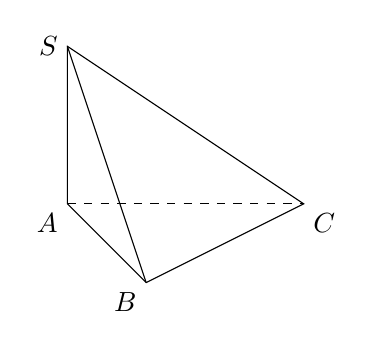
\begin{tikzpicture}
		\draw (0,0)--(1,-1)--(3,0)--(0,2)--cycle; 
		\draw[dashed]  (0,0)--(3,0);
		\draw (0,2)--(1,-1); 
		\node[below  left] at (0,0) {$A$};
		\node[below left]at (1,-1)  {$B$};
		\node[below right]at  (3,0) {$C$};
		\node[left]at (0,2)  {$S$};
	\end{tikzpicture}
	} 
\end{ex}

% nguồn: Ok_TracNghiemLop11_Lan1
\begin{ex}%[1H8N6-1]%[ma:4f5af152]
	\immini{ Cho hình chóp $S.ABC$  có $SA\perp \left(ABC\right)$. Góc giữa đường thẳng $SB$ và mặt phẳng $\left(ABC\right)$ là góc nào sau đây?
	\choice 
		{\True  $\widehat{SBA}$}
		{$\widehat{SCA}$} 
		 {$\widehat{SAC}$}
		 {$\widehat{SAB}$}
	\loigiai{ 
	 }}{
	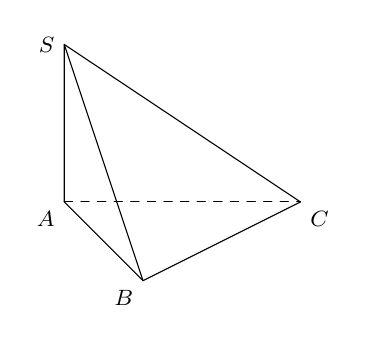
\begin{tikzpicture}[scale=1,font=\footnotesize,line join=round,line cap=round,>=stealth]
			\draw (0,0)--(1,-1)--(3,0)--(0,2)--cycle; 
			 \draw[dashed] (0,0)--(3,0);
			\draw  (0,2)--(1,-1);
			\node[below  left] at (0,0) {$A$};
			\node[below  left]at (1,-1) {$B$};
			\node[below right]at (3,0)  {$C$};
			\node[left]at  (0,2) {$S$};
		\end{tikzpicture}
	 }
\end{ex}

% nguồn: Ok_TracNghiemLop11_Lan1
\begin{ex}%[1H8N6-1]%[ma:35cbc5c0]
	Nếu  đường thẳng $a$ không vuông góc với mặt phẳng $(P)$ thì góc giữa đường thẳng $a$ và mặt phẳng $(P)$ là
	\choice 
		{góc giữa $a$ và đường thẳng $a'$ vuông góc với  $(P)$}
		{\True góc giữa $a$  và hình chiếu $a'$ của $a$ trên $(P)$}
		{góc giữa $a$ và đường thẳng $a'$ nằm  trong với $(P)$}
		{góc giữa $a$ và đường  thẳng $a'$ song song với $(P)$}
	 \loigiai{
		Nếu đường thẳng $a$ không vuông góc với mặt phăng $(P)$ thì góc giữa đường thẳng $a$ và mặt phẳng $P)$ là góc giữa  $a$ và hình chiếu $a'$ của $a$ trên $(P)$.
	} 
\end{ex}

% nguồn: Ok_TracNghiemLop11_Lan1
\begin{ex}%[1H8N6-1]%[ma:76d6137b]
	Cho hình chóp $S.ABCD$ có đáy là hình chữ nhật và $SA\perp \left(ABCD\right)$. Góc giữa đường thẳng $SD$  và mặt phẳng $\left(ABCD\right)$ là góc nào sau đây?
	 \choice
		{\True $\widehat{SDA}$} 
		{$\widehat{DSA}$} 
		 {$\widehat{SCD}$}
		{$\widehat{SDC}$} 
	\immini{  \loigiai{
		$AD$ là hình chiếu của $SD$ lên mặt phẳng $\left(ABCD\right)$  $\Rightarrow \left(\widehat{SD,\left(ABCD\right)}\right)=\left(\widehat{SD,AD}\right)=\widehat{SDA}$.
		 }
		}{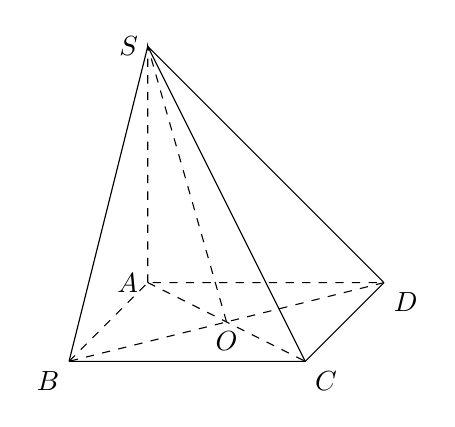
\begin{tikzpicture}
		\draw  (3,0)--(2,-1)--(-1,-1);
		\draw[dashed] (-1,-1)--(0,0)--(3,0); 
		\draw[dashed] (0,0)--(2,-1) 
			(3,0)--(-1,-1); 
		\draw[dashed]  (1,-.5)--(0,3)--(0,0);
		\draw  (-1,-1)--(0,3)--(2,-1)
			 (3,0)--(0,3);
		\node[left] at (0,0)  {$A$};
		\node[below left]at (-1,-1) {$B$}; 
		\node[below right]at (3,0) {$D$}; 
		\node[below right]at (2,-1) {$C$}; 
		\node[left]at (0,3)  {$S$};
		 \node[below]at (1,-.5) {$O$};
	\end{tikzpicture}
	 }
\end{ex}

% nguồn: Ok_TracNghiemLop11_Lan1
\begin{ex}%[1H8N6-1]%[ma:5150af8b]
	\immini{ Cho hình chóp tứ giác đều $S.ABCD$ có đáy là hình vuông tâm $O$. Góc giữa đường thẳng $SA$ và mặt phẳng  $\left(SBD\right)$ là góc nào sau đây?
	\choice 
		{\True  $\widehat{ASO}$}
		{$\widehat{ASB}$} 
		 {$\widehat{ASD}$}
		 {$\widehat{AOS}$}
	 \loigiai{
	 }}{
	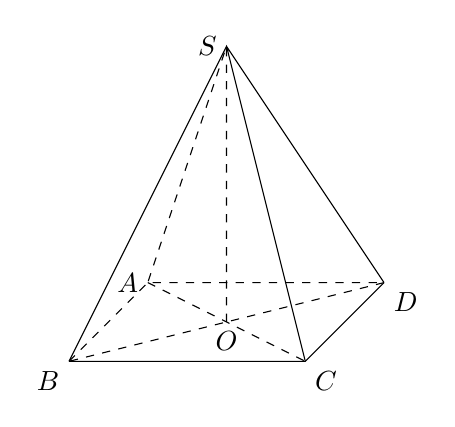
\begin{tikzpicture}
			\draw  (3,0)--(2,-1)--(-1,-1);
			\draw[dashed] (-1,-1)--(0,0)--(3,0); 
			\draw[dashed]  (0,0)--(2,-1)
				(3,0)--(-1,-1); 
			\draw[dashed]  (1,-.5)--(1,3)--(0,0);
			\draw  (-1,-1)--(1,3)--(2,-1)
				 (3,0)--(1,3);
			\node[left] at (0,0)  {$A$};
			 \node[below left]at (-1,-1) {$B$};
			 \node[below right]at (3,0) {$D$};
			\node[below right]at (2,-1)  {$C$};
			 \node[left]at (1,3) {$S$};
			\node[below]at (1,-.5) {$O$}; 
		\end{tikzpicture}
	} 
\end{ex}

% nguồn: Ok_Toan11_TracNghiem_Lan2
\begin{ex}%[1H8H6-1]%[ma:1d0687cb]
	Cho hình chóp $S.ABC$ có $SA$ vuông góc với mặt phẳng $\left(ABC\right)$. $SA=\sqrt{2} a$, tam giác $ABC$ vuông cân tại $B$ và $AB=a$. Góc giữa đường  thẳng $SC$ và mặt phẳng $\left(ABC\right)$ bằng
	 \choice
		{\True  $45^\circ$}
		 {$60^\circ$}
		{$30^\circ$} 
		 {$90^\circ$}
	 \loigiai{
		\begin{center}
			\begin{tikzpicture}[line join=round,line cap=round]
					 \coordinate (A) at (-2,0);
					\coordinate (B)  at (0,-1.5);
					\coordinate (C) at (3,0); 
					\coordinate (S) at  ($(A)+(0,3.5)$);
					\draw  (S)--(A)
						(S)--(B) 
						 (S)--(C)
						 (B)--(C)
						(A)--(B); 
					\draw pic[draw,angle  radius=0.5cm]{angle=S--C--A};
					 \draw[dashed,thin](A)--(C);
					\pic[draw,thin,angle radius=2mm] {right angle  = S--A--B} pic[draw,thin,angle radius=2mm] {right angle = S--A--C}
						pic[draw,thin,angle radius=2mm] {right angle = A--B--C}; 
					\foreach \i/\g in  {S/90,A/180,B/-90,C/0}{\draw[fill=white](\i) circle (1pt)
						 ($(\i)+(\g:3mm)$) node[scale=1]{$\i$};}
				\end{tikzpicture}
		\end{center}
		Vì tam  giác $ABC$ vuông cân tại $B$ $\Rightarrow AC=\sqrt{AB^2+BC^2}=a\sqrt{2}$.\\
		Ta  có $\left(\widehat{SC,\left(ABC\right)}\right)=\widehat{SCA}$.\\
		Mà $\tan \widehat{SCA}=\dfrac{SA}{AC}=\dfrac{a\sqrt{2}}{a\sqrt{2}}=1$ $\Rightarrow  \widehat{SCA}=45^\circ$.
	 }
\end{ex}

% nguồn: Ok_Toan11_TracNghiem_Lan2
\begin{ex}%[1H8H6-1]%[ma:48a68288]
	\immini{Cho hình chóp tứ giác đều $S.ABCD$ có tất cả các cạnh bằng $a$. Gọi $M$ là trung điểm của $SD$. Tang  của góc giữa đường thẳng $BM$ và mặt phẳng $(ABCD)$ bằng
	\choice 
		 {$\dfrac{\sqrt{2}}{2}$}
		{$\dfrac{\sqrt{3}}{3}$} 
		 {$\dfrac{2}{3}$}
		{\True $\dfrac{1}{3}$}}{ 
		\begin{tikzpicture}
				 \def\a{4}
				\def\h{4.5} 
				\path (0:0) coordinate (A) 
					++(0:\a)  coordinate (D)
					++(-130:\a/2) coordinate  (C)
					($(A)+(C)-(D)$) coordinate (B) 
					(intersection of A--C and  B--D) coordinate (O)
					($(O)+(90:\h)$) coordinate  (S)
					($(S)!1/2!(D)$)  coordinate (M);
				\draw[dashed]  (B)--(A)--(D)
					(A)--(S) 
					(B)--(M); 
				\draw (B)--(C)--(D) 
					(B)--(S) 
					(C)--(S) 
					 (D)--(S);
				\foreach \x/\g in {A/135,B/-135,C/-45,D/45,S/90,M/30} 
				\fill (\x) circle (1pt) 
					($(\g:3mm)+(\x)$) node  {$\x$};
			\end{tikzpicture}
		} 
	\loigiai{ 
		\begin{center}
			\begin{tikzpicture}
					 \def\a{4}
					 \def\h{4.5}
					\path (0:0) coordinate  (A)
						 ++(0:\a) coordinate (D)
						++(-130:\a/2) coordinate  (C)
						($(A)+(C)-(D)$) coordinate  (B)
						(intersection of A--C  and B--D) coordinate (O)
						($(O)+(90:\h)$)  coordinate (S)
						($(S)!1/2!(D)$) coordinate (M) 
						($(O)!1/2!(D)$) coordinate  (H);
					\draw[dashed]  (B)--(A)--(D)
						(A)--(S) 
						 (B)--(M)
						(A)--(C) 
						(B)--(D) 
						(S)--(O) 
						 (M)--(H);
					\draw  (B)--(C)--(D)
						 (B)--(S)
						 (C)--(S)
						(D)--(S); 
					 \foreach \x/\g in {A/135,B/-135,C/-45,D/45,S/90,O/-90,M/30,H/-60}
					\fill (\x)  circle (1pt)
						($(\g:3mm)+(\x)$)  node {$\x$};
					 \draw pic[draw,angle radius=6pt]{right angle=D--O--S};
				\end{tikzpicture}
		\end{center}
		Gọi $O$  là tâm của hình vuông.\\
		Ta có $SO  \perp(ABCD)$ và $SO = \sqrt{a^2 - \dfrac{a^2}{2}} = \dfrac{a\sqrt{2}}{2}$.\\
		Gọi $M$ là trung điểm của  $OD$.\\
		Ta có $MH\parallel SO$ nên $H$ là hình chiếu của $M$ lên mặt  phẳng $(ABCD)$ và $MH = \dfrac{1}{2}SO = \dfrac{a\sqrt{2}}{4}$.\\
		Do đó góc giữa đường thẳng $BM$ và mặt phẳng  $(ABCD)$ là $\widehat{MBH}$.\\
		Khi đó ta có  $\tan\widehat{MBH} = \dfrac{MH}{BH} = \dfrac{\dfrac{a\sqrt{2}}{4}}{\dfrac{3a\sqrt{2}}{4}} = \dfrac{1}{3}$.\\
	Vậy tang của góc giữa đường thẳng $BM$ và mặt phẳng  $(ABCD)$ bằng $\dfrac{1}{3}$.}
\end{ex}

% nguồn: Ok_Toan11_TracNghiem_Lan2
\begin{ex}%[1H8H6-1]%[ma:751a76ac]
	Cho hình chóp $S.ABC$ có $SA$ vuông góc với mặt phẳng $\left(ABC\right)$, $SA=a\sqrt{3}$, tam giác $ABC$ đều  cạnh có độ dài bằng $a$. Gọi $\alpha=\left(AB,\left(SBC\right)\right)$, khi đó $\sin \alpha$ bằng
	\choice 
		 {$\dfrac{\sqrt{5}}{3}$}
		{\True  $\dfrac{\sqrt{15}}{5}$}
		{$\dfrac{\sqrt{3}}{5}$} 
		 {$\dfrac{\sqrt{15}}{3}$}
	 \loigiai{
		\begin{center}
			\begin{tikzpicture}[line cap=round,line join=round,font=\footnotesize,declare function={a=3.5; b=2; h=3; goc=-40;}]
					 \path
						 (0:0) coordinate (A)
						(goc:b) coordinate  (B)
						(0:a) coordinate  (C)
						 (0,h) coordinate (S)
						 ($(B)!0.5!(C)$) coordinate (M)
						($(S)!(A)!(M)$)  coordinate (K);
					 \draw[dashed]
						 (A)--(C)
						 (M)--(A)--(K);
					\draw 
						 (S)--(A)--(B)--cycle--(C)--(B)
						(S)--(M) 
					\foreach \x/\y/\z  in {A/M/B,A/K/S}{
						pic[draw,angle radius  = 6pt]{right angle = \x--\y--\z}
						 };
					\foreach \x/\g  in {A/180,B/180,C/0,S/90,M/0,K/30}
					\fill (\x) circle (1pt) 
						 +(\g:3.5mm) node {$\x$};
				\end{tikzpicture}
		\end{center}
		Gọi $M$ là trung điểm  $BC$.\\ Kẻ đường cao $AK$ của tam giác $SAM$.\\
		Tam giác $ABC$ đều $\Rightarrow AM\perp BC\Rightarrow BC\perp \left(SAM\right)\Rightarrow  AK\perp \left(SBC\right)$.\\
		Suy ra $\alpha=\left(AB,\left(SBC\right)\right)=\left(AB,KB\right)=\widehat{ABK}$.\\ 
		Xét  tam giác $ABM$ vuông tại $A$ có
		\[\dfrac{1}{AK^2}=\dfrac{1}{SA^2}+\dfrac{1}{AM^2}=\dfrac{1}{\left(a\sqrt{3} \right)^2}+\dfrac{1}{\left(\dfrac{a\sqrt{3}}{2} \right)^2}=\dfrac{5}{3a^2} \Leftrightarrow AK=\dfrac{a\sqrt{15}}{5}.\] 
		Vì $AK\perp \left(SBC\right)\Rightarrow AK\perp BK$.\\ Xét tam giác $ABK$ vuông tại $K$ có $\sin  \alpha=\sin \widehat{ABK}=\dfrac{AK}{AB}=\dfrac{\sqrt{15}}{5}$.
	} 
\end{ex}

% nguồn: Ok_Toan11_TracNghiem_Lan2
\begin{ex}%[1H8H6-1]%[ma:55d98e99]
	\immini{Cho hình hộp chữ nhật $ABCD.A'B'C'D'$ có $AB=AD=2$ và $AA'=2\sqrt{2}$ (tham khảo hình bên). Góc giữa đường thẳng $CA'$ và mặt  phẳng $(ABCD)$ bằng
	 \choice
		 {$30^\circ$}
		{\True $45^\circ$} 
		{$60^\circ$} 
		 {$90^\circ$}}{
		\begin{tikzpicture}
				 \def\a{3.5}
				 \def\b{2}
				 \def\h{3}
				\path (0:0) coordinate (A) 
					++(0:\a) coordinate  (D)
					++(-130:\b) coordinate (C) 
					($(A)+(C)-(D)$) coordinate (B) 
					 ($(A)+(90:\h)$) coordinate (A')
					($(B)+(90:\h)$) coordinate  (B')
					($(C)+(90:\h)$) coordinate (C') 
					($(D)+(90:\h)$) coordinate  (D');
				\draw[dashed] (B)--(A)--(D) 
					(A)--(A')--(C); 
				\draw  (C)--(C')
					 (D)--(D')
					 (B)--(B')
					(C)--(C') 
					(B)--(C)--(D) 
					(A')--(B')--(C')--(D')--cycle; 
				\foreach \x/\g in  {A/180,B/180,C/0,D/0,A'/180,B'/180,C'/0,D'/0}
				\fill (\x) circle  (1pt)
					($(\g:4mm)+(\x)$) node {$\x$}; 
			\end{tikzpicture}
		 }
	\loigiai{Góc cần tìm là  $\widehat{A'CA}=\alpha$.\\
	Vì đáy là hình vuông  nên $AC=AB\cdot\sqrt{2}=2\sqrt{2}$ và $$\tan \alpha = \dfrac{AA'}{AC}=1 \Rightarrow \alpha=45^\circ.$$}
\end{ex}

% nguồn: Ok_Toan11_TracNghiem_Lan2
\begin{ex}%[1H8H6-1]%[ma:29efd0f0]
	Cho hình chóp  $S.ABCD$ có đáy là hình vuông cạnh $a$, $SA$ vuông góc với mặt phẳng đáy và $SB=2a$. Góc giữa đường thẳng $SB$ và mặt phẳng đáy bằng
	 \choice
		 {\True$60^\circ$}
		 {$90^\circ$}
		 {$30^\circ$}
		{$45^\circ$} 
	\loigiai{\begin{center}
		\begin{tikzpicture}
				\def\a{4} 
				 \def\h{3}
				\path (0:0) coordinate (A) 
					 ++(0:\a) coordinate (D)
					++(-130:\a/2) coordinate  (C)
					 ($(A)+(C)-(D)$) coordinate (B)
					($(A)+(90:\h)$) coordinate (S) 
					(intersection of  A--C and B--D) coordinate (O);
				\draw[dashed] (B)--(A)--(D) 
					(A)--(S); 
				\draw (B)--  (C)--(D)
					(B)--(S) 
					 (C)--(S)
					(D)--(S); 
				\foreach \x/\g in  {A/135,B/-135,C/-45,D/45,S/90}
				\fill (\x) circle  (1pt)
					($(\g:3mm)+(\x)$) node  {$\x$};
				\draw pic[draw,angle radius=6pt]{right angle=D--A--S}; 
			\end{tikzpicture}
	\end{center}
	Do $SA \perp(ABCD)$ nên góc giữa đường  thẳng $SB$ và mặt phẳng đáy bằng góc $\widehat{SBA}$.\\
	Ta có $\cos\widehat{SBA} = \dfrac{AB}{SB} = \dfrac{1}{2}  \Rightarrow \widehat{SBA} = 60^\circ$.\\
Vậy góc giữa đường thẳng $SB$ và  mặt phẳng đáy bằng $60^\circ$.}
\end{ex}

% nguồn: Ok_Toan11_TracNghiem_Lan2
\begin{ex}%[1H8H6-1]%[ma:e4ae50b8]
	\immini{ Cho hình chóp $S.ABC$ có đáy là tam giác vuông tại B, $AB=3a$, $BC=\sqrt{3}a$, $SA$  vuông góc với mặt phẳng đáy và $SA=2a$. Góc giữa đường thẳng $SC$ và mặt phẳng đáy bằng
	\choice 
		{$60^\circ$} 
		 {$45^\circ$}
		{\True $30^\circ$} 
		{$90^\circ$}}{ 
		\begin{tikzpicture}
				 \def\a{4}
				\def\h{3} 
				\path (0:0) coordinate (A) 
					++(0:\a) coordinate  (B)
					 ++(-150:4*\a/5) coordinate (C)
					 ($(A)+(90:\h)$) coordinate (S)
					($(A)!0.5!(B)$) coordinate  (M);
				\draw  (A)--(C)--(B)
					 (A)--(S)
					(B)--(S) 
					(C)--(S); 
				 \draw[dashed] (A)--(B);
				\foreach \x /\goc in {A/180,B/0,C/-135,S/90} 
				\fill  (\x) circle (1pt)
					($(\x)+(\goc:3mm)$)  node {$\x$};
				\draw pic[draw,angle radius=2mm]{right  angle=B--A--S};
			\end{tikzpicture}
		} 
	\loigiai{Ta có $SA \perp(ABC)$ nên  góc giữa $SC$ và $(ABC)$ bằng $\widehat{SCA}$.\\ $$AC=\sqrt{AB^2+BC^2}=\sqrt{9a^2+3a^2}=2a\sqrt{3}.$$
	Suy ra $\tan \widehat{ASC}=\dfrac{SA}{AC}=\dfrac{2a}{2a\sqrt{3}}=\dfrac{1}{\sqrt{3}}  \Rightarrow \widehat{SAC}=30^\circ$.}
\end{ex}

% nguồn: Ok_Toan11_TracNghiem_Lan2
\begin{ex}%[1H8H6-1]%[ma:ef3505cb]
	Cho hình chóp $S.ABC$ có $SA$ vuông góc với mặt phẳng $\left(ABC\right)$, $SA=2a$, tam giác $ABC$ vuông tại $B$, $AB=a\sqrt{3}$  và $BC=a$. Góc giữa đường thẳng $SC$ và mặt phẳng $\left(ABC\right)$ bằng
	 \choice
		 {$90^\circ$}
		{\True  $45^\circ$}
		{$30^\circ$} 
		{$60^\circ$} 
	\loigiai{ 
		\begin{center}
			\begin{tikzpicture}[line join=round,line cap=round]
					\coordinate (A)  at (-2,0);
					\coordinate (B) at  (0,-1.5);
					 \coordinate (C) at (3,0);
					\coordinate (S)  at ($(A)+(0,3.5)$);
					\draw (S)--(A) 
						 (S)--(B)
						(S)--(C) 
						 (B)--(C)
						(A)--(B); 
					\draw  pic[draw,angle radius=0.5cm]{angle=S--C--A};
					 \draw[dashed,thin](A)--(C);
					\pic[draw,thin,angle radius=2mm] {right angle  = S--A--B} pic[draw,thin,angle radius=2mm] {right angle = S--A--C}
						pic[draw,thin,angle radius=2mm]  {right angle = A--B--C};
					 \foreach \i/\g in {S/90,A/180,B/-90,C/0}{\draw[fill=white](\i) circle (1pt)
						 ($(\i)+(\g:3mm)$) node[scale=1]{$\i$};}
				\end{tikzpicture}
		\end{center}
		Ta thấy hình chiếu vuông góc của $SC$ lên $\left(ABC\right)$  là $AC$ nên $\left(\widehat{SC,\left(ABC\right)}\right)=\widehat{SCA}$.\\
		Mà $AC=\sqrt{AB^2+BC^2}=2a$  nên $\tan \widehat{SCA}=\dfrac{SA}{AC}=1$.\\
		Vậy góc giữa đường thẳng $SC$ và mặt phẳng $\left(ABC\right)$  bằng $45^\circ$.
	 }
\end{ex}

% nguồn: Ok_Toan11_TracNghiem_Lan2
\begin{ex}%[1H8H6-1]%[ma:dd81754b]
	Cho hình lăng trụ đứng $ABC.A'B'C'$ có đáy $ABC$ vuông tại $A$, $AB=a\sqrt{3}$, $AC=AA'=a$. Giá trị sin của góc giữa đường thẳng $AC'$ và mặt phẳng  $\left(BCC'B'\right)$ bằng
	\choice 
		 {$\dfrac{\sqrt{10}}{4}$}
		{$\dfrac{\sqrt{6}}{3}$} 
		{$\dfrac{\sqrt{3}}{3}$} 
		{\True $\dfrac{\sqrt{6}}{4}$} 
	\loigiai{ 
		\begin{center}
			\begin{tikzpicture}[scale=1,line cap=round,line join=round,font=\footnotesize,declare function={a=3.5; b=2; h=4; goc=-40;}]
					\path 
						(0:0) coordinate  (A')
						(0:a)  coordinate (C')
						 (goc:b) coordinate (B')
						(0,h) coordinate  (A)
						 ($(B')+(0,h)$) coordinate (B)
						($(C')+(0,h)$)  coordinate (C)
						($(B)!0.6!(C)$) coordinate  (H);
					\draw[dashed] 
						 (A')--(C')
						 (A)--(C');
					 \draw
						 (A)--(B)--(C)--(C')--(B')--(A')--cycle
						(A)--(C) 
						(B)--(B') 
						(A)--(H)--(C'); 
					\foreach \x/\g  in {A/180,B/-30,C/0,A'/-180,B'/-90,C'/0,H/-30}
					\fill (\x) circle  (1pt)
						+(\g:3mm)  node {$\x$};
				\end{tikzpicture}
		\end{center}
		Hạ $AH\perp BC$, ta có $AH\perp \left(BCC'B'\right)$.\\  Do đó $\left(AC', \left(BCC'B'\right)\right)=\widehat{AC'H}$.\\
		Trong tam giác  $ABC$, ta có $\dfrac{1}{AH^2}=\dfrac{1}{AB^2}+\dfrac{1}{AC^2}=\dfrac{4}{3a^2} \Rightarrow AH=\dfrac{a\sqrt{3}}{2}$.\\
		 Vậy $\sin \widehat{AC'H}=\dfrac{AH}{AC'}=\dfrac{a\sqrt{3}}{2a\sqrt{2}}=\dfrac{\sqrt{6}}{4}$.
	 }
\end{ex}

% nguồn: Ok_Toan11_TracNghiem_Lan2
\begin{ex}%[1H8H6-1]%[ma:5b0cbb52]
	Cho hình chóp $S.ABC$ có $SA$ vuông góc  với mặt phẳng $\left(ABC\right)$, $SA=\sqrt{2} a$, tam giác $ABC$ vuông cân tại $B$ và $AC=2a$. Góc giữa đường thẳng $SB$ và mặt phẳng $\left(ABC\right)$ bằng
	 \choice
		 {$30^\circ$}
		{\True $45^\circ$} 
		 {$60^\circ$}
		{$90^\circ$} 
	\loigiai{ 
		\begin{center}
			\begin{tikzpicture}[line join=round,line cap=round]
					\coordinate  (A) at (-2,0);
					\coordinate (B)  at (0,-1.5);
					\coordinate  (C) at (3,0);
					\coordinate  (S) at ($(A)+(0,3.5)$);
					 \draw (S)--(A)
						 (S)--(B)
						(S)--(C) 
						 (B)--(C)
						(A)--(B); 
					\draw  pic[draw,angle radius=0.5cm]{angle=S--B--A};
					\draw[dashed,thin](A)--(C); 
					\pic[draw,thin,angle radius=2mm] {right angle = S--A--B} pic[draw,thin,angle radius=2mm] {right angle =  S--A--C}
						pic[draw,thin,angle radius=2mm] {right  angle = A--B--C};
					\foreach \i/\g  in {S/90,A/180,B/-90,C/0}{\draw[fill=white](\i) circle (1pt)
						($(\i)+(\g:3mm)$) node[scale=1]{$\i$};} 
				\end{tikzpicture}
		\end{center}
		Ta có $SB\cap  \left(ABC\right)=B$; $SA\perp \left(ABC\right)$ tại $A$.\\
		Suy ra hình chiếu vuông góc của $SB$ lên mặt phẳng $\left(ABC\right)$ là  $AB$.\\
		Góc giữa đường thẳng $SB$ và mặt phẳng $\left(ABC\right)$  là $\alpha=\widehat{SBA}$.\\
		Do tam giác $ABC$ vuông cân  tại $B$ và $AC=2a$ nên $AB=\dfrac{AC}{\sqrt{2}}=\sqrt{2} a=SA$.\\
		Suy ra tam giác $SAB$ vuông cân tại $A$.\\ 
		Do  đó $\alpha=\widehat{SBA}=45^\circ$.\\
		 Vậy góc giữa đường thẳng $SB$ và mặt phẳng $\left(ABC\right)$ bằng $45^\circ$.
	} 
\end{ex}

% nguồn: Ok_Toan11_TracNghiem_Lan2
\begin{ex}%[1H8H6-1]%[ma:29b80dc6]
	Cho hình chóp $S.ABCD$ có đáy là hình vuông cạnh $a\sqrt{3}$, $SA$ vuông góc  với mặt phẳng đáy và $SA=a\sqrt{2}$. Góc giữa đường thẳng $SC$ và mặt phẳng $\left(ABCD\right)$ bằng
	 \choice
		 {$45^\circ$}
		 {\True $30^\circ$}
		 {$60^\circ$}
		 {$90^\circ$}
	\loigiai{ 
		\begin{center}
			\begin{tikzpicture}[line join=round,line cap=round]
					\coordinate (A) at  (0,0);
					\coordinate (B)  at (-1.5,-2);
					\coordinate (D) at  (5,0);
					\coordinate (C)  at ($(B)+(D)-(A)$);
					\coordinate (S) at ($(A)+(0,3.5)$); 
					\draw (S)--(B) 
						(S)--(C) 
						 (S)--(D)
						 (B)--(C)--(D);
					 \draw[dashed,thin](S)--(A)--(C)
						 (D)--(A)--(B);
					\draw  pic[draw,angle radius=0.5cm]{angle=S--C--A};
					\pic[draw,thin,angle radius=6pt] {right angle = S--A--D} pic[draw,thin,angle radius=6pt]  {right angle = S--A--B};
					 \foreach \i/\g in {S/90,A/-90,B/-90,C/-90,D/0}{\draw[fill=white](\i) circle (1pt)
						($(\i)+(\g:3mm)$) node[scale=1]{$\i$};} 
				\end{tikzpicture}
		\end{center}
		Vì $SA\perp \left(ABCD\right)$  nên $AC$ là hình chiếu của $SC$ trên mặt phẳng $\left(ABCD\right)$.\\
		 Do đó góc giữa đường thẳng $SC$ và mặt phẳng $\left(ABCD\right)$ là $\widehat{SCA}$.\\
		Đáy $ABCD$ là hình  vuông cạnh $a\sqrt{3}$ cho nên $AC=a\sqrt{6}$.\\
		Ta có  $\tan \widehat{SCA}=\dfrac{SA}{AC}=\dfrac{a\sqrt{2}}{a\sqrt{6}}=\dfrac{1}{\sqrt{3}}$.\\
		Vậy $\widehat{SCA}=30^\circ$. 
	 }
\end{ex}

% nguồn: Ok_Toan11_TracNghiem_Lan2
\begin{ex}%[1H8H6-1]%[ma:16f44c05]
	Cho hình chóp $S.ABC$ có $SA=SB=SC=\dfrac{a\sqrt{3}}{2}$, đáy là tam giác vuông tại $A$,  cạnh $BC=a$. Côsin của góc giữa đường thẳng $SA$ và mặt phẳng $\left(ABC\right)$ bằng
	 \choice
		 {\True $\dfrac{\sqrt{3}}{3}$}
		{$\dfrac{1}{3}$} 
		 {$\dfrac{\sqrt{3}}{2}$}
		 {$\dfrac{\sqrt{5}}{5}$}
	 \loigiai{
		\begin{center}
			\begin{tikzpicture}[line cap=round,line join=round,font=\footnotesize,declare function={a=3.5; b=2; h=3; goc=-40;}]
					\path 
						(0:0) coordinate (B) 
						 (0:a) coordinate (A)
						(goc:b) coordinate (C) 
						 ($(B)!0.5!(C)$) coordinate (H) ++ (0,h) coordinate (S);
					 \draw[dashed]
						(B)--(A)--(H); 
					\draw 
						(S)--(B)--(C)--cycle--(H) 
						 (S)--(A)--(C)
					\foreach \x/\y/\z in {S/H/B}{ 
						pic[draw,angle radius = 6pt]{right  angle = \x--\y--\z}
						}; 
					\foreach \x/\g  in {A/0,B/180,C/-45,S/90,H/180}
					\fill (\x)  circle (1pt)
						 +(\g:3.5mm) node {$\x$};
				\end{tikzpicture}
		\end{center}
		Gọi $H$ là hình chiếu vuông góc  của $S$ lên $\left(ABC\right)$.\\
		Do $SA=SB=SC$ nên $H$ là tâm đường tròn ngoại  tiếp tam giác $ABC$ hay $H$ là trung điểm của $BC\Rightarrow AH=\dfrac{a}{2}$.\\
		Ta có $\left(SA,\left(ABC\right)\right)=\left(SA,HA\right)=\widehat{SAH}=\alpha  \Rightarrow \cos \alpha=\dfrac{AH}{SA}=\dfrac{\sqrt{3}}{3}$.
	} 
\end{ex}

% nguồn: Ok_Toan11_TracNghiem_Lan2
\begin{ex}%[1H8H6-1]%[ma:f00c981c]
	Cho hình chóp $S.ABCD$ có đáy $ABCD$ là hình thoi cạnh $a$, $O$ là giao điểm  của $AC$ và $BD$, $\widehat{ABC}=60^{\circ}$; $SO$ vuông góc với $\left(ABCD\right)$ và $SO=a\sqrt{3}$. Góc giữa đường thẳng $SB$ và mặt phẳng $\left(SAC\right)$ nằm trong khoảng nào sau đây?
	\choice 
		{$\left(53^{\circ}; 61^{\circ} \right)$} 
		 {$\left(62^{\circ}; 66^{\circ} \right)$}
		 {$\left(27^{\circ}; 33^{\circ} \right)$}
		{\True $\left(25^{\circ};  27^{\circ} \right)$}
	\loigiai{ 
		\begin{center}
			\begin{tikzpicture}[line cap=round,line join=round,font=\footnotesize,declare function={a=3.5; b=2; h=3.5; goc=-135;}]
					 \path
						(0:0) coordinate  (A)
						 (0:a) coordinate (B)
						(goc:b) coordinate (D) 
						 ($(B)+(D)-(A)$) coordinate (C)
						($(A)!0.5!(C)$) coordinate (O)++(0,h) coordinate  (S);
					\draw[dashed] 
						(A)--(B) 
						 (A)--(D)--(B)
						(C)--(A)--(S)--(O); 
					\draw 
						 (D)--(C)--(B)
						 (S)--(B)
						(S)--(C) 
						(S)--(D) 
					\foreach  \x/\y/\z in {S/O/B,S/O/A}{
						pic[draw,angle  radius = 6pt]{right angle = \x--\y--\z}
						}; 
					\foreach \x/\g in  {A/135,B/0,C/-45,D/-135,S/90,O/-90}
					\fill  (\x) circle (1pt)
						+(\g:3.5mm) node  {$\x$};
				\end{tikzpicture}
		\end{center}
		Ta có  $BD\perp AC$ và $BD\perp SO$
		nên $BD\perp \left(SAC\right)\Rightarrow  \left(SBD\right)\perp \left(SAC\right)$.\\
		Mà $\left(SBD\right)\cap \left(SAC\right)=SO$ $\Rightarrow  \left(\widehat{SB,\left(SAC\right)}\right)=\left(\widehat{SB,SO}\right)=\widehat{BSO}$.\\
		 Ta có $\tan \widehat{BSO}=\dfrac{OB}{SO}=\dfrac{\dfrac{a\sqrt{3}}{2}}{a\sqrt{3}}=\dfrac{1}{2} \Rightarrow \widehat{BSO}\approx 26{,}56^{\circ}$.
	} 
\end{ex}

% nguồn: Ok_Toan11_TracNghiem_Lan2
\begin{ex}%[1H8H6-1]%[ma:4ec8e455]
	Cho hình lăng trụ đứng $ABC.A'B'C'$ có đáy $ABC$ là tam giác vuông cân tại $A$, $BC=AA'=a\sqrt{2}$. Tính tang của góc giữa đường thẳng $BC'$ và mặt phẳng $\left(ABB'A'\right)$. 
	 \choice
		 {$\dfrac{\sqrt{2}}{2}$}
		 {$\dfrac{\sqrt{6}}{3}$}
		{$\sqrt{2}$} 
		{\True  $\dfrac{\sqrt{3}}{3}$}
	\loigiai{ 
		\begin{center}
			\begin{tikzpicture}[scale=1,line cap=round,line join=round,font=\footnotesize,declare function={a=3.5; b=2; h=3; goc=-50;}]
					\path 
						(0:0)  coordinate (A')
						(0:a) coordinate (C') 
						(goc:b)  coordinate (B')
						(0,h) coordinate (A) 
						($(B')+(0,h)$)  coordinate (B)
						($(C')+(0,h)$) coordinate (C); 
					 \draw[dashed]
						 (A')--(C');
					\draw 
						(A)--(B)--(C)--(C')--(B')--(A')--cycle 
						(A)--(C) 
						(C')--(B)--(B'); 
					\foreach \x/\g in {A/180,B/90,C/0,A'/-180,B'/-90,C'/0} 
					 \fill (\x) circle (1pt)
						+(\g:3mm)  node {$\x$};
				\end{tikzpicture}
		\end{center}
		$\triangle  ABC$ vuông cân tại $A$ có $BC=a\sqrt{2}$ $\Rightarrow AB=AC=a$.\\
		$\triangle ABA'$ vuông  tại $A$ $\Rightarrow A'B=a\sqrt{3}$.\\
		Ta có $\heva{&C'A'\perp A'B'\\&C'A'\perp AA'}\Rightarrow C'A'\perp \left(ABB'A'\right)$.\\ 
		Suy ra $BA'$ là hình  chiếu của $BC'$ lên mặt phẳng $\left(ABB'A'\right)$.\\
		 Do đó $\left(BC',\left(ABB'A'\right)\right)=\left(BC',BA'\right)=\widehat{A'BC'}$.\\
		 $\triangle A'BC'$ vuông tại $A'\Rightarrow \tan \widehat{A'BC'}=\dfrac{A'C'}{A'B}=\dfrac{a}{a\sqrt{3}}=\dfrac{\sqrt{3}}{3}$.
	 }
\end{ex}

% nguồn: Ok_Toan11_TracNghiem_Lan2
\begin{ex}%[1H8H6-1]%[ma:ec423048]
	 Cho hình chóp tam giác đều $S.ABC$ có độ dài cạnh đáy là $2a$, $SA=3a$. Tính sin của góc giữa $BC$ và mặt phẳng $\left(SAB\right)$.
	\choice 
		{\True $\dfrac{\sqrt{46}}{8}$} 
		{$\dfrac{\sqrt{23}}{8}$} 
		{$\dfrac{\sqrt{46}}{4}$} 
		{$\dfrac{\sqrt{23}}{4}$} 
	\loigiai{ 
		\begin{center}
			\begin{tikzpicture}[line cap=round,line join=round,font=\footnotesize,declare function={a=4; b=2; h=3; goc=-50;}]
					\path 
						 (0:0) coordinate (A)
						(goc:b)  coordinate (B)
						(0:a) coordinate  (C)
						($(B)!0.5!(C)$)  coordinate (M)
						($(A)!2/3!(M)$) coordinate (H)++(0,h)  coordinate (S);
					 \draw[dashed]
						 (A)--(C)
						 (S)--(H)
						 (A)--(M);
					\draw 
						 (S)--(A)--(B)--cycle--(C)--(B)
					\foreach \x/\y/\z in  {A/H/S}{
						pic[draw,angle radius = 6pt]{right  angle = \x--\y--\z}
						 };
					 \foreach \x/\g in {A/180,B/180,C/0,S/90,H/-90,M/-30}
					\fill  (\x) circle (1pt)
						+(\g:3.5mm) node {$\x$}; 
				\end{tikzpicture}
		\end{center}
		Gọi $H$ là hình chiếu của $S$  xuống đáy và $M$ là trung điểm của $BC$.
		\[AH=\dfrac{2}{3}  AM=\dfrac{2}{3}\cdot\dfrac{2\sqrt{3}}{2} a=\dfrac{2\sqrt{3}}{3} a.\]
		Chiều  cao $SH=\sqrt{SA^2-AH^2}=\sqrt{(3a)^2-\left(\dfrac{2\sqrt{3}}{3} a\right)^2}=\dfrac{\sqrt{69}}{3} a$.\\
		Diện  tích tam giác $ABC$: $S_{ABC}=\dfrac{AB^2\sqrt{3}}{4}=\sqrt{3} a^2$.\\
		Thể tích khối chóp $S.ABC=\dfrac{1}{3}\cdot SH\cdot  S_{ABC}=\dfrac{\sqrt{23}}{3} a^3$.\\
		Diện tích tam giác $SAB$: $S_{SAB}=\sqrt{p\left(p-SA\right)\left(p-SB\right)\left(p-AB\right)}=2\sqrt{2}  a^2$.\\
		Khoảng cách từ $C$ đến mặt phẳng $\left(SAB\right)$  là $\mathrm{d}\left[C,\left(SAB\right)\right]=\dfrac{3V_{S.ABC}}{S_{ABC}}=\dfrac{\sqrt{46}}{4} a$.\\
		Sin góc giữa $BC$ và mặt  phẳng $\left(SAB\right)$: $\sin\alpha=\dfrac{\mathrm{d}\left[C,\left(SAB\right)\right]}{BC}=\dfrac{\sqrt{46}}{8}$.
	 }
\end{ex}

% nguồn: Ok_Toan11_TracNghiem_Lan2
\begin{ex}%[1H8H6-1]%[ma:0fd33ed8]
	\immini{Cho hình chóp $S.ABC$ có $SA$ vuông góc với mặt phẳng $(ABC)$, $SA=2a$, tam giác $ABC$ vuông cân tại $B$ và  $AB=\sqrt{2}a$ (minh họa như hình vẽ bên). Góc giữa đường thẳng $SC$ và mặt phẳng $(ABC)$ bằng
	 \choice
		 {$60^\circ$}
		{\True $45^\circ$} 
		 {$30^\circ$}
		 {$90^\circ$}}{
		\begin{tikzpicture}
				\def\a{4} 
				\def\h{3} 
				\path  (0:0) coordinate (A)
					++(0:\a) coordinate (B) 
					++(-150:4*\a/5) coordinate (C) 
					($(A)+(90:\h)$)  coordinate (S)
					($(A)!0.5!(B)$)  coordinate (M);
				\draw  (A)--(C)--(B)
					 (A)--(S)
					(B)--(S) 
					(C)--(S); 
				 \draw[dashed] (A)--(B);
				\foreach \x /\goc  in {A/180,B/0,C/-135,S/90}
				 \fill (\x) circle (1pt)
					($(\x)+(\goc:3mm)$) node  {$\x$};
				 \draw pic[draw,angle radius=2mm]{right angle=B--A--S};
			\end{tikzpicture}
		 }
	\loigiai{Ta có $$\heva{&SC  \cap(ABC) =C \\& SA \perp(ABC)} \Rightarrow(SC,(ABC)) =(\widehat{SC, AC}) =\widehat{SCA}.$$ Mà $AC=\sqrt{AB^2+BC^2}=\sqrt{(\sqrt{2}a)^2+(\sqrt{2}a)^2}=\sqrt{2a^2+2a^2}=\sqrt{4a^2}=2a=SA$.\\
	 Vì $\triangle SAC$ vuông cân tại $A$ nên ta có $\widehat{SCA}=45^\circ$.}
\end{ex}

% nguồn: Ok_Toan11_TracNghiem_Lan2
\begin{ex}%[1H8H6-1]%[ma:f6e78dc7]
	Cho hình chóp $S.ABCD$ có đáy là hình vuông cạnh $a$, $SA$ vuông góc với mặt phẳng  đáy và $SA=\sqrt{2}a$. Góc giữa đường thẳng $SC$ và mặt phẳng đáy bằng
	 \choice
		{\True $45^\circ$} 
		{$60^\circ$} 
		{$30^\circ$} 
		 {$90^\circ$}
	\loigiai{ 
		\begin{center}
			\begin{tikzpicture}[line join=round,line cap=round]
					 \coordinate (A) at (0,0);
					\coordinate  (B) at (-1.5,-2);
					 \coordinate (D) at (5,0);
					\coordinate (C) at  ($(B)+(D)-(A)$);
					 \coordinate (S) at ($(A)+(0,3.5)$);
					 \draw (S)--(B)
						 (S)--(C)
						 (S)--(D)
						(B)--(C)--(D); 
					 \draw[dashed,thin](S)--(A)--(C)
						(D)--(A)--(B); 
					 \draw pic[draw,angle radius=0.5cm]{angle=S--C--A};
					\pic[draw,thin,angle radius=6pt] {right angle = S--A--D}  pic[draw,thin,angle radius=6pt] {right angle = S--A--B};
					\foreach \i/\g in {S/90,A/-90,B/-90,C/-90,D/0}{\draw[fill=white](\i) circle  (1pt)
						($(\i)+(\g:3mm)$)  node[scale=1]{$\i$};}
				\end{tikzpicture}
		\end{center}
		Do $SA\perp \left(ABCD\right)$ nên góc giữa đường thẳng $SC$ và mặt phẳng đáy bằng góc $\widehat{SCA}$.\\ 
		Ta có  $SA=\sqrt{2}a$, $AC=\sqrt{2}a$ $\Rightarrow \tan \widehat{SCA}=\dfrac{SA}{AC}$ $=1$ $\Rightarrow \widehat{SCA}=45^\circ$.\\
		Vậy góc giữa đường thẳng $SC$ và mặt phẳng  đáy bằng bằng $45^\circ$.
	} 
\end{ex}

% nguồn: Ok_Toan11_TracNghiem_Lan2
\begin{ex}%[1H8H6-1]%[ma:eed14b60]
	Cho hình chóp $S.ABC$ có đáy là tam giác vuông tại $C$, $AC=a$, $BC=\sqrt{2}a$, $SA$  vuông góc với mặt phẳng đáy và $SA=a$. Góc giữa đường thẳng $SB$ và mặt phẳng đáy bằng
	\choice 
		 {$60^\circ$}
		 {$90^\circ$}
		{\True  $30^\circ$}
		 {$45^\circ$}
	\loigiai{ 
		\begin{center}
			\begin{tikzpicture}[line join=round,line cap=round]
					\coordinate  (A) at (-2,0);
					\coordinate (C)  at (0,-1.5);
					\coordinate (B)  at (3,0);
					 \coordinate (S) at ($(A)+(0,3.5)$);
					\draw (S)--(A) 
						(S)--(B) 
						 (S)--(C)
						 (B)--(C)
						 (A)--(C);
					 \draw pic[draw,angle radius=0.5cm]{angle=S--B--A};
					\draw[dashed,thin](A)--(B); 
					\pic[draw,thin,angle radius=2mm] {right angle = S--A--B} pic[draw,thin,angle radius=2mm] {right angle  = S--A--C}
						pic[draw,thin,angle radius=2mm] {right  angle = A--C--B};
					\foreach \i/\g in {S/90,A/180,B/0,C/-90}{\draw[fill=white](\i)  circle (1pt)
						 ($(\i)+(\g:3mm)$) node[scale=1]{$\i$};}
				\end{tikzpicture}
		\end{center}
		Có $SA\perp \left(ABC\right)$ nên $AB$ là hình chiếu của $SA$ trên mặt phẳng $\left(ABC\right)$.  Suy ra
		\[\left(\widehat{SB,\left(ABC\right)}\right)=\left(\widehat{SB,AB}\right)=\widehat{SBA}.\] 
		 Mặt khác có $\triangle ABC$ vuông tại $C$ nên $AB=\sqrt{AC^2+BC^2}=a\sqrt{3}$.\\
		Khi đó $\tan \widehat{SBA}=\dfrac{SA}{AB}=\dfrac{1}{\sqrt{3}}$ nên $\left(\widehat{SB,\left(ABC\right)}\right)=30^\circ$. 
	} 
\end{ex}

% nguồn: Ok_Toan11_TracNghiem_Lan2
\begin{ex}%[1H8H6-1]%[ma:0d23994c]
	Cho hình chóp $S.ABC$ có đáy $ABC$ là tam giác vuông tại $B$, $AB=a$, $BC=2a$, $SA$ vuông góc với mặt phẳng đáy và $SA=\sqrt{15} a$. Góc giữa đường thẳng $SC$ và  mặt phẳng đáy bằng
	\choice 
		 {$45^\circ$}
		 {$30^\circ$}
		 {\True $60^\circ$}
		 {$90^\circ$}
	\loigiai{ 
		\begin{center}
			\begin{tikzpicture}[line join=round,line cap=round]
					\coordinate (A) at  (-2,0);
					\coordinate (B) at (0,-1.5); 
					\coordinate (C) at (3,0); 
					\coordinate (S)  at ($(A)+(0,3.5)$);
					 \draw (S)--(A)
						(S)--(B) 
						(S)--(C) 
						(B)--(C) 
						(A)--(B); 
					\draw pic[draw,angle  radius=0.5cm]{angle=S--C--A};
					\draw[dashed,thin](A)--(C); 
					\pic[draw,thin,angle radius=2mm] {right  angle = S--A--B} pic[draw,thin,angle radius=2mm] {right angle = S--A--C}
						pic[draw,thin,angle radius=2mm] {right  angle = A--B--C};
					\foreach \i/\g in  {S/90,A/180,B/-90,C/0}{\draw[fill=white](\i) circle (1pt)
						($(\i)+(\g:3mm)$)  node[scale=1]{$\i$};}
				\end{tikzpicture}
		\end{center}
		Do $SA$ vuông góc với mặt phẳng đáy  nên $AC$ là hình chiếu vuông góc của $SC$ lên mặt phẳng đáy.\\
		Suy ra $\left(\widehat{SC,  \left(ABC\right)}\right)=\left(\widehat{SC, AC}\right)=\widehat{SCA}$.\\
		Trong tam giác $ABC$ vuông  tại $B$ ta có $AC=\sqrt{AB^2+BC^2}=\sqrt{a^2+4a^2}=\sqrt{5} a$.\\
		Trong tam giác $SAC$ vuông  tại $A$ ta có $\tan \widehat{SCA}=\dfrac{SA}{AC}=\dfrac{\sqrt{15} a}{\sqrt{5} a}=\sqrt{3}$ $\Rightarrow \widehat{SCA}=60^\circ$.\\
	Vậy $\left(\widehat{SC,  \left(ABC\right)}\right)=60^\circ$.}
\end{ex}

% nguồn: Ok_Toan11_TracNghiem_Lan2
\begin{ex}%[1H8H6-1]%[ma:7ffe47f4]
	\immini{Cho hình lập  phương $ABCD.A'B'C'D'$ (tham khảo hình bên). Giá trị $\sin$ của góc giữa đường thẳng $AC'$ và mặt phẳng $(ABCD)$ bằng
	\choice 
		 {\True $\dfrac{\sqrt{3}}{3}$}
		 {$\dfrac{\sqrt{6}}{3}$}
		{$\dfrac{\sqrt{3}}{2}$} 
		 {$\dfrac{\sqrt{2}}{2}$}}{
		\begin{tikzpicture}
				 \def\a{3.5}
				\path (0:0) coordinate (A) 
					++(0:\a) coordinate (D) 
					 ++(-130:\a/2) coordinate (C)
					 ($(A)+(C)-(D)$) coordinate (B)
					($(A)+(90:\a)$) coordinate  (A')
					 ($(B)+(90:\a)$) coordinate (B')
					($(C)+(90:\a)$)  coordinate (C')
					($(D)+(90:\a)$) coordinate  (D');
				\draw[dashed]  (B)--(A)--(D)
					(A)--(A') 
					(A)--(C') 
					(A)--(C); 
				 \draw (C)--(C')
					(D)--(D') 
					(B)--(B') 
					(B)--(C)--(D) 
					 (A')--(B')--(C')--(D')--cycle;
				 \foreach \x/\g in {A/180,B/180,C/0,D/0,A'/180,B'/180,C'/0,D'/0}
				\fill  (\x) circle (1pt)
					 ($(\g:4mm)+(\x)$) node {$\x$};
			\end{tikzpicture}
		} 
	\loigiai{ Ta có $\left(\widehat{AC',(ABCD) }\right)=\widehat{(AC', AC) }=\widehat{C'AC}=\alpha$.\\ 
		Giả sử hình lập phương  có cạnh là $a$.\\
	Trong tam  giác $A'AC$ ta có $$\sin\alpha=\dfrac{CC'}{AC'}=\dfrac{a}{\sqrt{2a^2+a^2}}=\dfrac{\sqrt{3}}{3}.$$}
\end{ex}

% nguồn: Ok_Toan11_TracNghiem_Lan2
\begin{ex}%[1H8H6-1]%[ma:40beb7e0]
	Cho hình chóp $S.ABC$ có đáy $ABC$ là tam giác vuông tại $B$, $AB=a$, $BC=a\sqrt{2}$, $SA$ vuông góc với mặt phẳng đáy và $SA=a$. Góc giữa đường thẳng $SC$ và  mặt phẳng đáy bằng
	 \choice
		{$90^\circ$} 
		{$45^\circ$} 
		{$60^\circ$} 
		 {\True $30^\circ$}
	\loigiai{ 
		\begin{center}
			\begin{tikzpicture}[line join=round,line cap=round]
					\coordinate (A)  at (-2,0);
					\coordinate (B) at (0,-1.5); 
					 \coordinate (C) at (3,0);
					 \coordinate (S) at ($(A)+(0,3.5)$);
					\draw (S)--(A) 
						 (S)--(B)
						 (S)--(C)
						(B)--(C) 
						 (A)--(B);
					 \draw pic[draw,angle radius=0.5cm]{angle=S--C--A};
					 \draw[dashed,thin](A)--(C);
					\pic[draw,thin,angle  radius=2mm] {right angle = S--A--B} pic[draw,thin,angle radius=2mm] {right angle = S--A--C}
						pic[draw,thin,angle radius=2mm] {right angle  = A--B--C};
					\foreach \i/\g in  {S/90,A/180,B/-90,C/0}{\draw[fill=white](\i) circle (1pt)
						 ($(\i)+(\g:3mm)$) node[scale=1]{$\i$};}
				\end{tikzpicture}
		\end{center}
		Ta có góc giữa $SC$ và mặt  phẳng đáy là góc $\widehat{SCA}$.\\
		Xét tam giác $SCA$ vuông tại $A$ ta  có\\
	$AC=\sqrt{AB^2+BC^2}=a\sqrt{3}$, $\tan \widehat{SCA}=\dfrac{SA}{AC}=\dfrac{a}{a\sqrt{3}} \Rightarrow  \widehat{SCA}=30^\circ.$}
\end{ex}

% nguồn: Ok_Toan11_TracNghiem_Lan2
\begin{ex}%[1H8H6-1]%[ma:16688b2b]
	Cho hình chóp $S.ABC$ có $SA$  vuông góc với mặt phẳng $\left(ABC\right)$, $SA=2a$, tam giác $ABC$ vuông tại $B$, $AB=a$, $BC=a\sqrt{3}$. Góc giữa đường thẳng $SC$ và mặt phẳng $\left(ABC\right)$ bằng
	\choice 
		 {$90^\circ$}
		{$30^\circ$} 
		 {$60^\circ$}
		{\True  $45^\circ$}
	 \loigiai{
		\begin{center}
			\begin{tikzpicture}[line join=round,line cap=round]
					\coordinate  (A) at (-2,0);
					 \coordinate (B) at (0,-1.5);
					\coordinate (C) at  (3,0);
					\coordinate (S) at ($(A)+(0,3.5)$); 
					 \draw (S)--(A)
						(S)--(B) 
						(S)--(C) 
						 (B)--(C)
						 (A)--(B);
					\draw  pic[draw,angle radius=0.5cm]{angle=S--C--A};
					 \draw[dashed,thin](A)--(C);
					\pic[draw,thin,angle radius=2mm] {right angle = S--A--B} pic[draw,thin,angle  radius=2mm] {right angle = S--A--C}
						pic[draw,thin,angle radius=2mm]  {right angle = A--B--C};
					\foreach \i/\g in {S/90,A/180,B/-90,C/0}{\draw[fill=white](\i) circle  (1pt)
						($(\i)+(\g:3mm)$)  node[scale=1]{$\i$};}
				\end{tikzpicture}
		\end{center}
		Ta có $SA$ vuông góc với mặt  phẳng $(ABC)$, suy ra $AC$ là hình chiếu của $SC$ lên mặt phẳng $(ABC)$.
		Do  đó $$\widehat{\left[SC,\left(ABC\right)\right]}=\widehat{\left(SC,AC\right)}=\widehat{SCA}.$$
		 $\triangle ABC$ vuông tại $B$ $\Rightarrow AC^2=AB^2+BC^2=a^2+3a^2=4a^2$ $\Rightarrow AC=2a$.
		$$\tan \widehat{SCA}=\dfrac{SA}{AC}=\dfrac{2a}{2a}=1\Rightarrow \widehat{SCA}=45^\circ  \Rightarrow \left(\widehat{SC,\left(ABC\right)}\right)=45^\circ.$$
	 }
\end{ex}

% nguồn: Ok_Toan11_TracNghiem_Lan2
\begin{ex}%[1H8H6-1]%[ma:7d4049a7]
	Cho hình chóp $S.ABC$ và có đáy $ABC$ là tam giác vuông tại  $B$, $AB=a$, $BC=3a$, $SA$ vuông góc với mặt phẳng đáy và $SA=\sqrt{30}a$. Góc giữa đường thẳng $SC$ và mặt phẳng đáy bằng
	 \choice
		{$45^\circ$} 
		 {$90^\circ$}
		{\True $60^\circ$} 
		{$30^\circ$} 
	 \loigiai{
		\begin{center}
			\begin{tikzpicture}[line join=round,line cap=round]
					\coordinate  (A) at (-2,0);
					\coordinate (B) at (0,-1.5); 
					 \coordinate (C) at (3,0);
					\coordinate (S)  at ($(A)+(0,3.5)$);
					\draw  (S)--(A)
						 (S)--(B)
						(S)--(C) 
						 (B)--(C)
						 (A)--(B);
					\draw  pic[draw,angle radius=0.5cm]{angle=S--C--A};
					 \draw[dashed,thin](A)--(C);
					\pic[draw,thin,angle  radius=2mm] {right angle = S--A--B} pic[draw,thin,angle radius=2mm] {right angle = S--A--C}
						pic[draw,thin,angle  radius=2mm] {right angle = A--B--C};
					\foreach  \i/\g in {S/90,A/180,B/-90,C/0}{\draw[fill=white](\i) circle (1pt)
						 ($(\i)+(\g:3mm)$) node[scale=1]{$\i$};}
				\end{tikzpicture}
		\end{center}
		Do $AC$ là  hình chiếu vuông góc của $SC$ trên mặt phẳng $\left(ABC\right)$ nên $\widehat{\left(SC,\left(ABC\right)\right)}=\widehat{SCA}$.\\
		 Ta có $AC=\sqrt{AB^2+BC^2}=a\sqrt{10}$.\\
		Khi đó $\tan SCA=\dfrac{SA}{AC}=\dfrac{a\sqrt{30}}{a\sqrt{10}}=\sqrt{3} \Rightarrow  \widehat{SCA}=60^\circ$.
	} 
\end{ex}

% nguồn: Ok_Toan11_TracNghiem_Lan2
\begin{ex}%[1H8H6-1]%[ma:93ba5ae6]
	Cho hình chóp $S.ABCD$ có $SA$ vuông góc với mặt phẳng đáy, $SA=a$, $ABCD$ là hình chữ  nhật và $AB=a$, $AD=a\sqrt{2}$. Góc giữa đường thẳng $SC$ và mặt phẳng $\left(ABCD\right)$ bằng
	 \choice
		{$90^{\circ}$} 
		{$60^{\circ}$} 
		 {$45^{\circ}$}
		{\True $30^{\circ}$} 
	\loigiai{ 
		\begin{center}
			\begin{tikzpicture}[line cap=round,line join=round,font=\footnotesize,declare function={a=3.5; b=2; h=3; goc=-135;}]
					 \path
						(0:0) coordinate (A) 
						(0:a)  coordinate (B)
						(goc:b) coordinate  (D)
						(0,h) coordinate  (S)
						($(B)+(D)-(A)$) coordinate (C); 
					 \draw[dashed]
						(A)--(B) 
						 (A)--(D)
						(C)--(A)--(S); 
					\draw 
						 (D)--(C)--(B)
						 (S)--(B)
						 (S)--(C)
						 (S)--(D)
					 \foreach \x/\y/\z in {S/A/B,S/A/D}{
						pic[draw,angle radius = 6pt]{right angle  = \x--\y--\z}
						}; 
					\foreach \x/\g  in {A/135,B/0,C/-45,D/-135,S/90}
					\fill  (\x) circle (1pt)
						+(\g:3.5mm)  node {$\x$};
				\end{tikzpicture}
		\end{center}
		Ta có $SA\perp \left(ABCD\right)\Rightarrow$  $AC$ là hình chiếu của $SC$ lên mặt phẳng $\left(ABCD\right)$.\\
		Suy ra  $\left(SC,\left(ABCD\right)\right)=\left(SC,AC\right)=\widehat{SCA}=\alpha$.\\
		 Mặt khác $AC=\sqrt{AB^2+BC^2}=\sqrt{a^2+2a^2}=a\sqrt{3}$.\\
		 Xét tam giác vuông $SAC$ có $\tan \alpha=\dfrac{SA}{AC}=\dfrac{a}{a\sqrt{3}}=\dfrac{1}{\sqrt{3}} \Rightarrow \alpha=30^{\circ}$.
	} 
\end{ex}

% nguồn: Ok_Toan11_TracNghiem_Lan2
\begin{ex}%[1H8H6-1]%[ma:d94a3dc2]
	 \immini{
	Cho hình chóp $S.ABCD$ có đáy là hình vuông cạnh bằng $2a$. Tam giác $SAB$ cân  tại $S$ và nằm trong mặt phẳng vuông góc với đáy. Biết thể tích khối chóp $S.ABCD$ bằng $\dfrac{4a^3}{3}$. Gọi $\alpha$ là góc giữa $SC$ và mặt đáy, tính $\tan \alpha$.
	 \choice
		 {$\tan \alpha =\dfrac{\sqrt{3}}{3}$}
		{$\tan \alpha  =\dfrac{2\sqrt{5}}{5}$}
		{$\tan  \alpha =\dfrac{\sqrt{7}}{7}$}
		 {\True $\tan \alpha =\dfrac{\sqrt{5}}{5}$}
		 }{
		\begin{tikzpicture}[scale=0.7,>=stealth,line join=round,line cap=round,font=\footnotesize]
				 \def\a{4}
				 \def\h{4}
				\def\r{2} 
				 \def\al{-145}
				\path 
					(0,0) coordinate  (A)
					(\al:\r) coordinate (B) 
					(\a,0)  coordinate (D)
					($(B)+(D)-(A)$) coordinate  (C)
					 ($(B)!1/2!(A)$) coordinate (H)
					($(H)+(0,\h)$)  coordinate (S);
				 \draw (S)--(B)--(C)--(S)--(D)--(C);
				\draw[dashed,thin]  (B)--(A)--(S)
					(A)--(D) 
					(S)--(H); 
				\foreach \p/\g  in {A/160,B/-120,C/-45,D/0,S/90,H/160}\fill (\p) circle (1pt) node[shift={(\g:.3)}]{$\p$};
				 \foreach \a/\b/\c in {S/H/A}
					{\draw pic[draw,angle  radius=2mm] {right angle = \a--\b--\c};};
			\end{tikzpicture}
		} 
	\loigiai{ 
	 \immini{
		Gọi $H$ là trung điểm  của $AB$, vì $\vartriangle SAB$ cân tại $S$ nên $SH\perp AB$.\\
		Ta có $\heva{&(SAB)\perp (ABCD) \\&(SAB)\cap (ABCD)=AB \\&SH\perp AB}\Rightarrow SH\perp  (ABCD)$.\\
		Suy  ra $(SC,(ABCD))=\alpha =\widehat{SCH}$.\\
		Ta có $$V_{S.ABCD}=\dfrac{1}{3}SH\cdot{S_{ABCD}}\Leftrightarrow\dfrac{1}{3}SH\cdot 4a^2=\dfrac{4a^3}{3}\Leftrightarrow SH=a.$$ 
		Ta có  $HC=\sqrt{BH^2+BC^2}=a\sqrt{5}$.\\
		Vậy $\tan \alpha  =\tan \widehat{SCH}$ $=\dfrac{SH}{HC}$ $=\dfrac{a}{a\sqrt{5}}$ $=\dfrac{\sqrt{5}}{5}$.
		 }{
		\begin{tikzpicture}[scale=0.7,>=stealth,line join=round,line cap=round,font=\footnotesize]
				 \def\a{4}
				 \def\h{4}
				 \def\r{2}
				\def\al{-145} 
				 \path
					(0,0) coordinate  (A)
					(\al:\r) coordinate (B) 
					(\a,0) coordinate (D) 
					($(B)+(D)-(A)$) coordinate  (C)
					($(B)!1/2!(A)$) coordinate (H) 
					($(H)+(0,\h)$)  coordinate (S);
				\draw (S)--(B)--(C)--(S)--(D)--(C); 
				\draw[dashed,thin] (B)--(A)--(S) 
					(A)--(D) 
					(S)--(H)--(C); 
				\foreach \p/\g  in {A/160,B/-120,C/-45,D/0,S/90,H/160}\fill (\p) circle (1pt) node[shift={(\g:.3)}]{$\p$};
				\foreach \a/\b/\c in  {S/H/A}
					{\draw pic[draw,angle radius=2mm] {right angle =  \a--\b--\c};};
			\end{tikzpicture}
		 }
	} 
\end{ex}

% nguồn: Ok_TracNghiemLop11_Lan1
\begin{ex}%[1H8H6-1]%[ma:93c6655b]
	Cho hình chóp $S.ABC$  có đáy $ABC$ là tam giác đều cạnh $a$. Hình chiếu vuông góc của $S$ lên $(ABC)$ trùng với trung điểm $H$ của cạnh $BC$. Biết tam giác $SBC$ là tam giác đều. Tính số đo của góc giữa $SA$ và $(ABC)$.
	 \choice
		 {$30^{\circ}$}
		{$45^{\circ}$} 
		 {\True $60^{\circ}$}
		 {$90^{\circ}$}
	\loigiai{ 
	\immini{Hình chiếu vuông góc của $SA$  lên $(ABC)$ là $HA$. \\
		Suy ra góc giữa $SA$  và $(ABC)$ là $\widehat{SAH}$ (vì $\widehat{SAH}<90^\circ$). \\
		Tam  giác $SAH$ vuông tại $H$ có $SH=AH=\dfrac{a\sqrt{3}}{2}$ nên là tam giác vuông cân tại $H$. \\
		Suy ra $\widehat{SAH}=45^\circ$.\\ 
		 Vậy góc giữa $SA$ và $(ABC)$ có số đo là $45^{\circ}$.}
		{ 
		\begin{tikzpicture}[scale=1,font=\footnotesize,line join=round,line cap=round,>=stealth]
				\coordinate[label=left:{$B$}]  (B) at (0,0);
				\coordinate[label=below:{$C$}]  (C) at (1.5,-1);
				\coordinate[label=right:{$A$}] (A) at  (4,0);
				\coordinate[label=below left:{$H$}]  (H) at ($(B)!0.5!(C)$);
				\coordinate[label={$S$}]  (S) at ($(H)+(0,3)$);
				\draw (C)--(A)--(S)--(C)--(B)--(S)--(H); 
				\draw[dashed]  (H)--(A)--(B);
				\foreach \x/\dinh/\y in {A/H/C,S/H/A} \draw[fill  = gray!50] ($(\dinh)!3pt!(\x)$)--($(\dinh)!3pt!(\x)+(\dinh)!3pt!(\y)-(\dinh)$)--($(\dinh)!3pt!(\y)$)--(\dinh)--cycle;
				\foreach \p in {A,B,C,H,S} 
				\fill (\p) circle  (1pt);
			\end{tikzpicture}
	}} 
\end{ex}

% nguồn: Ok_TracNghiemLop11_Lan1
\begin{ex}%[1H8H6-1]%[ma:234147e7]
	Cho hình  lăng trụ đứng $ABC.A'B'C'$ có đáy $ABC$ là tam giác đều cạnh $a$. Khi đó góc giữa $AC$ và mặt phẳng $ABB'A'$ bằng
	\choice 
		{\True  $60^\circ$}
		 {$75^\circ$}
		{$45^\circ$} 
		 {$30^\circ$}
	 \loigiai{
		\begin{center}
			\begin{tikzpicture}[scale=1,font=\footnotesize,line join=round,line cap=round,>=stealth]
					\path 
						 (0,3) coordinate[label=left: A'] (A')
						(0,0) coordinate[label=left:  A] (A)
						(3,0) coordinate[label=right: C]  (C)
						(3,3) coordinate[label=right:  C'] (C')
						(1,2) coordinate[label=left: B'] (B') 
						 (1,-1) coordinate[label=left: B] (B)
						 ($(A)!.5!(B)$) coordinate[label=left: H] (H);
					\draw  (A')--(B')--(C')--cycle;
					\draw (B)--(B')--(C')--(C)--cycle; 
					 \draw (A')--(A)--(B);
					\draw[dashed] (A)--(C)--(H); 
				\end{tikzpicture}
		\end{center}
		Gọi $H$ là trung điểm  $AB$
		Ta có $CH \perp AB$ nên $AH$  là hình chiếu vuông góc của $AC$ lên mặt phẳng $(ABB'A')$
		Do đó, $  (AC,(ABB'A'))=(AC,AH)=\widehat{CAB}$
		Mặt khác, tam giác $ABC$ đều nên $\widehat{CAB}=60^{\circ}$ hay  $(AC,(ABB'A'))60^{\circ}$
	} 
\end{ex}

% nguồn: Ok_TracNghiemLop11_Lan1
\begin{ex}%[1H8H6-1]%[ma:3624f345]
	Cho  hình lập phương $ABCD.A'B'C'D'$. Góc giữa hai đường thẳng $A'C'$ và $BD$ bằng
	\choice 
		{$60^{\circ}$} 
		 {$30^{\circ}$}
		{$45^{\circ}$} 
		{\True  $90^{\circ}$}
	 \loigiai{
	\immini{Ta  có $(A'C',BD)=(AC,BD)=90^{\circ}$.}{
		\begin{tikzpicture}[scale=.8,>=stealth,font=\footnotesize,line join=round,line cap=round]
				\def\a{3.5} 
				\path (0:0)  coordinate (A)
					++(0:\a) coordinate (D) 
					++(-130:\a/2) coordinate (C) 
					 ($(A)+(C)-(D)$) coordinate (B)
					 ($(A)+(90:\a)$) coordinate (A')
					($(B)+(90:\a)$) coordinate (B') 
					($(C)+(90:\a)$) coordinate (C') 
					($(D)+(90:\a)$) coordinate (D'); 
				 \draw[dashed] (B)--(A)--(D)
					(A)--(A') 
					(A)--(C) 
					 (B)--(D);
				\draw[thick] (A')--(C') 
					(C)--(C') 
					(D)--(D') 
					 (B)--(B')
					 (B)--(C)--(D)
					(A')--(B')--(C')--(D')--cycle; 
				\foreach \x/\g  in {A/180,B/180,C/0,D/0,A'/180,B'/180,C'/0,D'/0}
				\fill[black]  (\x) circle (1pt)
					($(\g:4mm)+(\x)$)  node {$\x$};
			\end{tikzpicture}
		} 
	 }
\end{ex}

% nguồn: Ok_TracNghiemLop11_Lan1
\begin{ex}%[1H8H6-1]%[ma:2b2d2f88]
	\immini{ Cho hình chóp $S.ABC$. Hình chiếu vuông góc của  $S$ lên $\left(ABC\right)$ trùng với trung điểm $H$ của cạnh $BC$. Biết tam giác $SBC$ là tam giác đều.
	 Tính số đo của góc giữa $SC$ và $\left(ABC\right)$.
	\choice 
		{\True $60^\circ$} 
		{$75^\circ$} 
		{$45^\circ$} 
		 {$30^\circ$}
	\loigiai{ 
		Từ giả thiết ta có $SH\perp \left(ABC\right)$ suy ra $HC$ là hình chiếu của $SC$ trên mặt phẳng  $\left(ABC\right)$.
		Do đó $\widehat{\left(SC,\left(ABC\right)\right)}=\widehat{\left(SC,HC\right)}=\widehat{SCH}=60^\circ$ (Do tam giác $SBC$ là tam giác đều). 
	}}{ 
	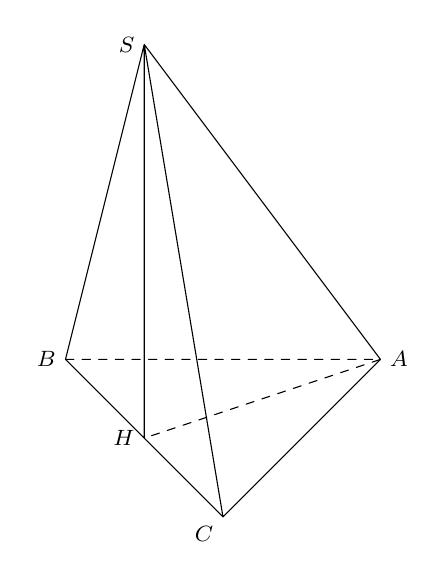
\begin{tikzpicture}[scale=1,font=\footnotesize,line join=round,line cap=round,>=stealth]
			\draw[dashed] (0,0)--(4,0)--(1,-1); 
			\draw (0,0)--(2,-2)--(4,0)--(1,4)--(1,-1) 
				(0,0)--(1,4)--(2,-2); 
			\node[right]  at (4,0) {$A$};
			\node[left] at  (0,0) {$B$};
			\node[below  left]at (2,-2) {$C$};
			\node[left]at (1,4)  {$S$};
			\node[left]at  (1,-1) {$H$};
		\end{tikzpicture}
	} 
\end{ex}

% nguồn: Ok_TracNghiemLop11_Lan1
\begin{ex}%[1H8H6-1]%[ma:6b30bb76]
	Cho hình chóp $S.ABCD$ có đáy $ABCD$ là hình vuông, $SA$ vuông góc với mặt phẳng đáy $(ABCD)$, Biết $SA=a \sqrt{2}$, $AB=a$.  Số đo của góc hợp bởi đường thẳng $SC$ và $(SAD)$ bằng
	\choice 
		 {\True $30^{\circ}$}
		{$45^{\circ}$} 
		 {$90^{\circ}$}
		{$60^{\circ}$.} 
	 \loigiai{
	\immini{Ta có  $\heva{
		& CD\perp  AD\quad\left( ABCD\,\text{là hình vuông} \right) \\
		&  CD\perp SA\quad\left(SA\perp (ABCD) \right)}
		 \Rightarrow CD\perp (SAD)$.\\
		Ta  có $SD$ là hình chiếu của $SC$ trên $(SAD)$.\\
		Khi đó $\left(SC,\left( SAD \right) \right)=\widehat{CSD}$.\\ 
		Xét $\triangle SCD$ ta có $\tan\widehat{CSD}=\dfrac{CD}{SD}=\dfrac{CD}{\sqrt{SA^2+AD^2}}=\dfrac{\sqrt{3}}{3}$.\\ 
		 Vậy $\left(SC,\left( SAD \right) \right)=\widehat{CSD}=30^\circ$.}
		{\begin{tikzpicture}[font=\footnotesize,line join=round,line cap=round,>=stealth,scale=0.6]
		 \path
			(0,0) coordinate (A) 
			(-2,-2)  coordinate (B)
			(3,-2)  coordinate (C)
			(5,0) coordinate (D) 
			 (0,4) coordinate (S);
		 \draw
			 (S)--(B)--(C)--(D)--cycle
			(S)--(C); 
		\draw [dashed] (S)--(A)--(D) 
			 (B)--(A);
		\draw  pic[draw,angle radius=15,angle eccentricity=1.5]{angle=C--S--D};
		\draw pic[draw,angle  radius=5,angle eccentricity=1.5]{right angle=S--A--D};
		\foreach \x/\g in 
			 {A/150,B/180,C/0,D/0,S/90}
		\fill[black](\x) circle (1pt) 
			($(\x)+(\g:3mm)$)  node{$\x$};
	\end{tikzpicture}
		 }
	 }
\end{ex}

% nguồn: Ok_TracNghiemLop11_Lan1
\begin{ex}%[1H8H6-1]%[ma:41b29dee]
	Cho hình chóp $S.ABCD$ có đáy $\left(ABCD\right)$ là hình vuông cạnh $a$. Cạnh bên $SA$ vuông góc với mặt phẳng đáy $\left(ABCD\right)$. Góc giữa cạnh $SC$ và mặt phẳng $\left(SAD\right)$ là góc  nào sau đây?
	\choice 
		 {$\widehat{SCA}$}
		{$\widehat{CSA}$} 
		 {$\widehat{SCD}$}
		{\True  $\widehat{CSD}$}
	 \loigiai{\immini{
		 Ta có $SC\cap \left(SAD\right)=\left\{S\right\} (1)$.
		 Mặt khác: $\heva{&CD\perp AD\\ &CD\perp SA \\ &AD\cap SA=\left\{A\right\}}$
		$\Rightarrow CD\perp \left(SAD\right)$, tức  là $D$ là hình chiếu vuông góc của $C$ lên $\left(SAD\right) (2)$.
		Từ $(1)$, $(2)$ suy ra $SD$ là hình chiếu vuông  góc của $SC$ lên $\left(SAD\right)$.
		Vậy góc giữa cạnh $SC$ và mặt phẳng $\left(SAD\right)$ là $\widehat{CSD}$.}{ 
		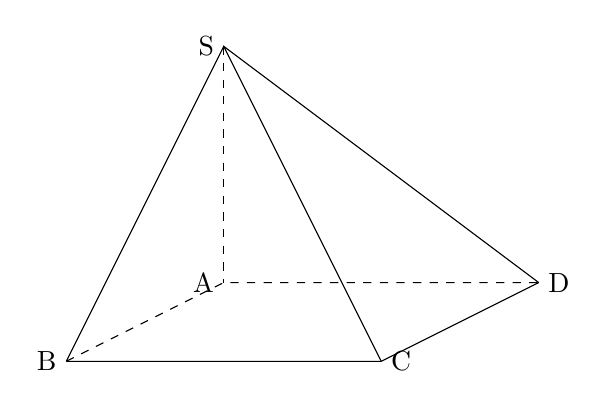
\begin{tikzpicture}
				 \path
					(0,3) coordinate[label=left:  S] (S)
					(0,0) coordinate[label=left: A] (A) 
					(2,-1) coordinate[label=right:  C] (C)
					(4,0) coordinate[label=right:  D] (D)
					(-2,-1) coordinate[label=left:  B] (B);
				 \draw (D)--(C)--(B);
				 \draw[dashed] (B)--(A)--(D);
				\draw[dashed] (S)--(A); 
				 \draw (B)--(S)--(C)
					(D)--(S); 
			\end{tikzpicture}
		} 
	} 
\end{ex}

% nguồn: Ok_TracNghiemLop11_Lan1
\begin{ex}%[1H8H6-1]%[ma:3f523a33]
	Cho hình chóp $S.ABCD$ có đáy là hình chữ nhật, $SA\perp (ABCD)$. Tính góc giữa đường thẳng $DC$  và mặt phẳng $(SAD)$.
	\choice 
		{$30^{\circ}$} 
		{$60^{\circ}$} 
		{$45^{\circ}$} 
		{\True  $90^{\circ}$}
	 \loigiai{
	\immini{Do $SA \perp (ABCD) \Rightarrow SA\perp CD$. Mặt khác $CD\perp AD$ suy ra $CD\perp (SAD)$. Khi  đó, $(CD,(SAD))=90^{\circ}.$
		 }
		{\begin{tikzpicture}[scale=1,font=\footnotesize,line join=round,line cap=round,>=stealth]
		 \path
			(0,0) coordinate  (A)
			(0:3) coordinate  (B)
			(-140:2)  coordinate (D)
			($(D)+(B)-(A)$) coordinate (C) 
			(90:3)  coordinate (S);
		 \draw (S)--(D)--(C)--(B)--(S)--(C);
		\draw[dashed]  (S)--(A)--(B)
			(A)--(D); 
		\foreach  \p/\q in {S/90,A/180,B/0,C/-90,D/-90}
		\fill[black]  (\p) circle (1.0pt) node[shift={(\q:3mm)}]{$\p$};
		 \draw pic[draw,angle radius=0.2cm] {right angle = S--A--D};
		\draw pic[draw,angle radius=0.2cm]  {right angle = S--A--B};
	\end{tikzpicture}
		 }
	 }
\end{ex}

% nguồn: Ok_TracNghiemLop11_Lan1
\begin{ex}%[1H8H6-1]%[ma:6b8076bf]
	Cho hình chóp $S.ABCD$ có đáy là hình thoi tâm $O$ cạnh $a$. $\triangle ABC$ cân tại $A$, $SA$ vuông góc với đáy. Tính góc giữa đường thẳng $BC$ với mặt  phẳng $\left(SAB\right)$.
	 \choice
		{$30^\circ$} 
		{$45^\circ$} 
		{\True  $60^\circ$}
		 {$90^\circ$}
	 \loigiai{
		\begin{center}
			\begin{tikzpicture}
					\path 
						(0,3) coordinate[label=left: S] (S) 
						 (0,0) coordinate[label=left: A] (A)
						(2,-2) coordinate[label=right: C]  (C)
						(4,0) coordinate[label=right: D]  (D)
						(-2,-2)  coordinate[label=left: B] (B)
						($(A)!0.5!(C)$) coordinate[label=left: O]  (O)
						($(A)!0.5!(B)$) coordinate[label=left: H]  (H);
					 \draw (D)--(C)--(B);
					 \draw[dashed] (B)--(A)--(D);
					\draw[dashed] (S)--(A) 
						(A)--(C) 
						(B)--(D) 
						 (C)--(H)--(S);
					\draw (B)--(S)--(C) 
						 (D)--(S);
				\end{tikzpicture}
		\end{center}
		Ta  có tam giác $ABC$ cân tại $A$ và $AB=BC$ (do ABCD là hình thoi).\\
		Nên ta có tam giác $ACB$  là tam giác đều.\\
		Gọi $H$  là trung điểm $AH$. Ta có $\heva{& CH \perp AB\\& CH \perp SA}$ (do $SA \perp (ABCD)$).\\
		Nên $BH$ là  hình chiêu vuông góc của $BC$ lên $(SAB)$.\\
		Vậy $(BC, (SAB))=(BC, BH)=\widehat{CBH}=60^{\circ}$ ( do tam giác $ABC$ đều) 
	 }
\end{ex}

% nguồn: Ok_TracNghiemLop11_Lan1
\begin{ex}%[1H8H6-1]%[ma:8ac80c6d]
	Cho hình chóp $S.ABCD$ có đáy $ABCD$ là  hình vuông cạnh $a$, cạnh bên $SA$ vuông góc với mặt phẳng $(ABCD)$, $SA=a\sqrt{2}$. Góc giữa đường thẳng $SC$ và mặt phẳng $(ABCD)$ bằng
	\choice 
		{\True $45^\circ$} 
		 {$30^\circ$}
		{$60^\circ$} 
		{$90^\circ$} 
	\loigiai{ 
	\immini{Ta có $AC$  là hình chiếu vuông góc của $SC$ lên mặt phẳng $(ABCD)$. Bởi vậy
		$$\widehat{\left(SC;(ABCD)\right)}=\widehat{\left(SC;AC\right)}=\widehat{SCA}.$$ 
		Ta có  $AC=SA=a\sqrt{2}$ nên suy ra tam giác $SAC$ vuông cân tại $A$, bởi vậy $\widehat{SCA}=45^\circ$.}
		{ 
		\begin{tikzpicture}[line cap=round,line join=round,>=stealth,scale=.8]
				 \path
					(0,0) coordinate (A) 
					($(A)+(-2,-1)$) coordinate (B) 
					($(A)+(4,0)$) coordinate  (D)
					($(B)+(D)-(A)$) coordinate  (C)
					($(A)+(0,3)$) coordinate (S); 
				 \draw[dashed](S)--(A)--(B)
					(C)--(A)--(D); 
				 \draw (S)--(B)--(C)--(D)--cycle (S)--(C);
				\foreach \p/\n in  {S/above,A/left,B/below,C/below,D/right}
				\fill  (\p) circle (1pt) node[\n]{$\p$};
				 \path pic[angle radius=2mm,draw,angle eccentricity=1.5] {right angle = S--A--C};
			\end{tikzpicture}
		 }
	 }
\end{ex}

% nguồn: Ok_TracNghiemLop11_Lan1
\begin{ex}%[1H8H6-1]%[ma:ff246107]
	Cho tam giác  $ABC$ vuông cân tại $A$ và $BC=a$. Trên đường thẳng qua $A$ vuông góc với $\left(ABC\right)$ lấy điểm $S$ sao cho $SA=\dfrac{a\sqrt{6}}{2}$. Tính số đo giữa đường thẳng $SB$ và $\left(SAC\right)$.
	\choice 
		{\True  $30^\circ$}
		 {$60^\circ$}
		 {$45^\circ$}
		 {$90^\circ$}
	 \loigiai{\immini{
		Có $\heva{&AB\perp SA \\  &AB\perp AC}$
		$\Rightarrow AB\perp \left(SAC\right)$,  suy ra $SA$ là hình chiếu vuông góc của $SB$ trên $\left(SAC\right)$.
		Vì tam giác $SAB$ vuông tại $A$ nên $\widehat{BSA}$ nhọn. 
		Suy ra góc  giữa $SB$ và $\left(SAC\right)$ bằng góc giữa $SB$ và $SA$ và bằng $\widehat{BSA}$.
		Tam giác $ABC$ vuông cân tại  $A$, suy ra $AB=\dfrac{BC}{\sqrt{2}}=\dfrac{a}{\sqrt{2}}$.
		Có $\tan \widehat{BSA}=\dfrac{AB}{SA}=\dfrac{1}{\sqrt{3}} \Rightarrow \widehat{BSA}=30^\circ$.} 
		{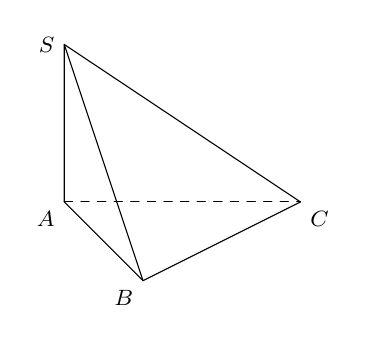
\begin{tikzpicture}[scale=1,font=\footnotesize,line join=round,line cap=round,>=stealth]
		 \draw (0,0)--(1,-1)--(3,0)--(0,2)--cycle;
		\draw[dashed] (0,0)--(3,0); 
		\draw  (0,2)--(1,-1);
		\node[below left]  at (0,0) {$A$};
		 \node[below left]at (1,-1) {$B$};
		 \node[below right]at (3,0) {$C$};
		 \node[left]at (0,2) {$S$};
	\end{tikzpicture}
		} 
	 }
\end{ex}

% nguồn: Ok_TracNghiemLop11_Lan1
\begin{ex}%[1H8H6-1]%[ma:6dd82200]
	Cho hình chóp $S.ABCD$ có đáy là hình vuông cạnh $a$, $SA \perp(ABCD)$ và $SA=a \sqrt{3}$. Góc  giữa đường thẳng $SD$ và mặt phẳng $(ABCD)$ bằng
	\choice 
		 {$45^\circ$}
		 {\True $60^\circ$}
		{$90^\circ$} 
		 {$30^\circ$}
	\loigiai{ 
	\immini{Vì $SA\bot (ABCD)$ nên hình chiếu của $SA$ lên đáy  là $AD$.\\
		Suy  ra $(SD;(ABCD))=\widehat{SDA}$.\\
		 Mà $\tan \widehat{SDA}=\dfrac{SA}{AD}=\dfrac{a\sqrt{3}}{a}=\sqrt{3}\Rightarrow \widehat{SDA} = 60^\circ$.\\
		Hay $(SD;(ABCD))=\widehat{SDA} = 60^\circ$.\\ 
		 }
		{	\begin{tikzpicture}[declare function={r=3; gd=-157;},font=\scriptsize]
		\path (0,0) coordinate  (A)
			(0:0.7*r) coordinate  (D)
			(90:r)  coordinate (S)
			(gd:0.4*r) coordinate  (B)
			($(B)+(D)-(A)$) coordinate  (C);
		\foreach \x/\y/\z in {S/A/B,S/A/D}{ 
			 \path pic[draw,angle radius=4pt,fill=cyan]{right angle= \x--\y--\z}; }
		 \draw (S)--(D)--(C)--(B)--cycle--(C);
		\draw[dashed] (S)--(A)--(B) 
			(A)--(D); 
		 \foreach \t/\g in {A/140,B/180,C/-60,D/0,S/90}{
			\fill (\t) circle (1pt) node[shift={(\g:7pt)}]{$ \t  $}; }
	\end{tikzpicture}
		 }
	} 
\end{ex}

% nguồn: Ok_TracNghiemLop11_Lan1
\begin{ex}%[1H8H6-1]%[ma:367feef3]
	\immini{Cho hình chóp $S.ABCD$  có đáy $ABCD$ là hình vuông, $O$ là giao điểm của $AC$ và $BD$. Biết rằng $SO$ vuông góc với mặt phẳng đáy (tham khảo hình bên). Góc giữa đường thẳng $SB$ và mặt phẳng $(ABCD)$ là
	\choice 
		{$\widehat{SOB}$} 
		 {$\widehat{SBA}$}
		{\True  $\widehat{SBO}$}
		{$\widehat{SBC}$}} 
		{\begin{tikzpicture}[=>stealth,line join=round,line cap=round,font=\footnotesize,scale=.7]
		 \def\a{5}
		\def\goc{210} 
		\def\b{3} 
		\def\h{4.5} 
		 \path
			(0,0) coordinate (A)++(0:\a) coordinate (B)++(\goc:\b) coordinate (C)++(180:\a)  coordinate (D)
			($(A)!.5!(C)$) coordinate  (O)
			(O)++(90:\h)  coordinate (S);
		\draw  (S)--(B)--(C)--(D)--cycle (S)--(C);
		\draw[dashed] (O)--(S)--(A)--(C) 
			(B)--(A)--(D) 
			 (B)--(D);
		\foreach \x/\g in{A/160,B/0,C/-90,S/90,O/-90,D/-90} 
		\fill[black](\x) circle  (1pt)
			($(\x)+(\g:3mm)$) node{$\x$}; 
	\end{tikzpicture}
		 }
	\loigiai{ 
		Có $SO \perp (ABCD)$ nên $OB$  là hình chiếu của $SB$ trên $(ABCD)$.\\
		 Khi đó $\widehat{(SB,(ABCD))}=\widehat{(SB,OB)}=\widehat{SBO}$.
	 }
\end{ex}

% nguồn: Ok_TracNghiemLop11_Lan1
\begin{ex}%[1H8H6-1]%[ma:6006667d]
	Cho hình chóp $S. ABC$ có $S A \perp(ABC)$ và $SA=AB$.  Góc giữa đường thẳng $SB$ và mặt phẳng $(ABC)$ bằng
	\choice 
		{$90^{\circ}$} 
		{\True  $45^{\circ}$}
		 {$30^{\circ}$}
		{$60^{\circ}$} 
	\loigiai{ 
	 \immini{
		Ta có $SA\perp  (ABC)\\
		\Rightarrow AB$  là hình chiếu vuông góc của $SB$ lên mặt phẳng $(ABC)$.\\
		 Suy ra $\widehat{(SB,(ABC))}=\widehat{SBA}$.\\
		Mà $\triangle SAB$ vuông cân tại $A$ nên  $\widehat{SBA} =45^\circ$.
		}{\begin{tikzpicture}
		 \def\a{3}
		\path (0:0) coordinate (A) 
			++(0:\a) coordinate  (B)
			++(-140:4*\a/5)  coordinate (C)
			 ($(A)+(90:\a)$) coordinate (S);
		 \draw (C)--(A)
			 (C)--(B)
			(A)--(S) 
			 (B)--(S)
			(C)--(S); 
		\draw[dashed]  (A)--(B);
		\foreach \x  / \goc in {A/180,B/0,C/-135,S/90}
		\fill (\x) circle  (1pt)
			($(\x)+(\goc:3mm)$) node  {$\x$};
		\draw  pic[draw,angle radius=2mm]{right angle=S--A--B}
			 pic[draw,angle radius=5mm]{angle=S--B--A};
	\end{tikzpicture}
		} 
	} 
\end{ex}

% nguồn: Ok_TracNghiemLop11_Lan1
\begin{ex}%[1H8H6-1]%[ma:e5648d44]
	Cho hình chóp $S.ABCD$ có đáy $ABCD$ là hình thang vuông tại $A$ và $D$ thỏa mãn $\dfrac{1}{2}AB=AD=CD$ và $SA$ vuông góc với mặt phẳng $(ABCD)$. Gọi $O$ là giao điểm của $AC$ và $BD$. Khi  đó góc hợp bởi $SB$ và mặt phẳng $(SAC)$ là
	\choice 
		 {$\widehat{DSO}$}
		{\True $\widehat{BSC}$} 
		 {$\widehat{BSO}$}
		 {$\widehat{BSA}$}
	\loigiai{ 
		\begin{center}
			\begin{tikzpicture}[scale=0.7]
					\coordinate (a)  at (0,0);
					\coordinate  (b) at (8,0);
					\coordinate (d)  at (-2,-3);
					 \coordinate (c) at (2,-3);
					\coordinate  (s) at ($(a)+(0,6)$);
					\coordinate  (o) at (intersection of a--c and b--d);
					\draw [dashed] (a) node[left]{$A$}--(b)  node[below]{$B$}
						(a)--(d)  node[below]{$D$}
						(s)  node[above]{$S$}--(a);
					\draw (b)--(c) node[below]{$C$} 
						(s)--(b) 
						(s)--(c)--(d)--cycle; 
					\draw [dashed]  (a)--(c)
						 (b)--(o) node[below]{$O$}--(d);
					\draw pic[draw,angle radius=0.2cm] {right angle  = b--a--d};
					\draw  pic[draw,angle radius=0.2cm] {right angle = a--d--c};
					\draw pic[draw,angle radius=0.2cm]  {right angle = a--c--b};
					 \coordinate (a') at (9,0);
					 \coordinate (b') at (15,0);
					 \coordinate (d') at (9,-3);
					 \coordinate (c') at (12,-3);
					\coordinate (m') at (12,0); 
					\coordinate (o') at  (intersection of a'--c' and b'--d');
					\draw (a') node[left]{$A$}--(b') node[right]{$B$}--(c') node[below]{$C$}--(d')  node[below]{$D$}--cycle (b')--(d')
						(a')--(o') node[above]{\  $O$}--(c')--(m') node[above]{$M$};
					\draw pic[draw,angle radius=0.2cm] {right angle =  b'--a'--d'};
					\draw pic[draw,angle radius=0.2cm] {right angle  = a'--d'--c'};
					\draw pic[draw,angle radius=0.2cm] {right angle  = b'--m'--c'};
					\draw pic[draw,angle radius=0.2cm] {right angle  = a'--c'--b'};
					\foreach \x  in {s,a,b,c,d,o,a',b',c',d',m'}{
						 \fill (\x) circle (1pt);
					 }
				\end{tikzpicture}
		\end{center}
		- Từ  $CM=MA=MB$ suy ra $BC\perp AC$.\\
		- Lại có $BC\perp  SA$, suy ra $BC\perp (SAC)$.\\
		- Hình chiếu của $SB$ lên  mặt phẳng $(SAC)$ là $SC$, do đó góc cần xác định là $\widehat{BSC}$.
	} 
\end{ex}

% nguồn: Ok_TracNghiemLop11_Lan1
\begin{ex}%[1H8H6-1]%[ma:53eb9053]
	\immini{ Cho hình chóp $S.ABCD$ đáy $ABCD$ là  hình vuông, cạnh bên $SA$ vuông góc với đáy, $SA=a\sqrt{3}$, $AB=a$. Tính góc giữa đường thẳng $SD$ và mặt phẳng $\left(SAB\right)$.
	 \choice
		 {\True $30^\circ$}
		 {$60^\circ$}
		 {$45^\circ$}
		{$90^\circ$} 
	 \loigiai{
		Ta  có $AD\perp AB.$ $ \quad (1)$
		Mặt khác $SA\perp \left(ABCD\right)$. 
		$\Rightarrow SA\perp AD$. $ \quad  (2)$
		Từ  $(1)$ và $(2)$ $\Rightarrow AD\perp \left(SAB\right)$.
		$\Rightarrow SA$ là hình chiếu của $SD$ lên $\left(SAB\right)$. 
		$\Rightarrow \widehat{\left(SD,\left(SAB\right)\right)}=\widehat{\left(SD,SA\right)}=\widehat{DSA}$. 
		Ta  có $\triangle SAD$ vuông tại $A$.
		$\Rightarrow \tan  \widehat{DSA}=\dfrac{AD}{SA}=\dfrac{1}{\sqrt{3}} \Rightarrow \widehat{DSA}=30^\circ$.
	 }}
	 {
	\begin{tikzpicture}
			 \path
				(0,3) coordinate[label=left: S] (S) 
				(0,0) coordinate[label=left:  A] (A)
				 (2,-1) coordinate[label=right: C] (C)
				(4,0) coordinate[label=right:  D] (D)
				 (-2,-1) coordinate[label=left: B] (B);
			\draw (D)--(C)--(B); 
			\draw[dashed] (B)--(A)--(D); 
			 \draw[dashed] (S)--(A);
			\draw (B)--(S)--(C) 
				(D)--(S); 
		\end{tikzpicture}
	} 
\end{ex}

% nguồn: Ok_TracNghiemLop11_Lan1
\begin{ex}%[1H8H6-1]%[ma:495c356c]
	Cho  hình chóp $S.ABCD$, đáy $ABCD$ là hình vuông cạnh bằng $a$ và $SA\perp \left(ABCD\right)$. Biết $SA=a\sqrt{2}$. Tính góc giữa $SC$ và $\left(SAB\right)$.
	 \choice
		{\True $30^\circ$} 
		{$45^\circ$} 
		{$60^\circ$} 
		{$75^\circ$} 
	 \loigiai{\immini{
		Ta có $SA\perp \left(ABCD\right)$ 
		$\Rightarrow SA\perp BC$. 
		 $ABCD$ là hình vuông
		$\Rightarrow  AB\perp BC$.
		Do đó $BC\perp  \left(SAB\right)$.
		 $\Rightarrow \widehat{\left(SC,\left(SAB\right)\right)}=\widehat{\left(SC,SB\right)}=\widehat{CSB}$.
		Ta có $\triangle SAB$ vuông,  suy ra
		\begin{align*}
			 SB&=\sqrt{SA^2+AB^2}\\
			&=\sqrt{\left(a\sqrt{2} \right)^2+a^2}=a\sqrt{3}. 
		\end{align*}
		$\Rightarrow \tan \widehat{CSB}=\dfrac{BC}{SB}=\dfrac{\sqrt{3}}{3} \Rightarrow \alpha=30^\circ$.} 
		 {
		\begin{tikzpicture}[scale=1,font=\footnotesize,line join=round,line cap=round,>=stealth]
				 \path
					(0,3)  coordinate[label=left: S] (S)
					(0,0) coordinate[label=left: A]  (A)
					(2,-1)  coordinate[label=right: C] (C)
					(4,0) coordinate[label=right: D] (D) 
					(-2,-1) coordinate[label=left: B] (B) 
					 ($(B)!.5!(D)$) coordinate[label=below: O] (O);
				\draw (D)--(C)--(B); 
				 \draw[dashed] (B)--(A)--(D);
				 \draw[dashed] (A)--(C)
					 (D)--(B);
				\draw[dashed] (O)--(S)--(A); 
				 \draw (B)--(S)--(C)
					(D)--(S); 
				\draw[dashed]  (A)--(S);
			\end{tikzpicture}
		 }
	} 
\end{ex}

% nguồn: Ok_TracNghiemLop11_Lan1
\begin{ex}%[1H8H6-1]%[ma:71a69f5c]
	\immini{Cho hình chóp $S.ABCD$  có đáy $ABCD$ là hình vuông cạnh $a$, cạnh bên $SA$ vuông góc với mặt phẳng đáy và $SA=a \sqrt{3}$ (tham khảo hình bên). Góc giữa đường thẳng $SB$ và mặt phẳng $(ABCD)$ bằng
	 \choice
		{$90^{\circ}$} 
		{\True $60^{\circ}$} 
		 {$30^{\circ}$}
		 {$45^{\circ}$}}
		{\begin{tikzpicture}[=>stealth,line join=round,line cap=round,font=\footnotesize,scale=.7]
		\def\a{4} 
		 \def\goc{210}
		\def\b{2.5} 
		 \def\h{4}
		\path 
			(0,0) coordinate (A)++(0:\a) coordinate (D)++(\goc:\b) coordinate (C)++(180:\a) coordinate  (B)
			(A)++(90:\h) coordinate (S); 
		\draw (S)--(B)--(C)--(D)--cycle (S)--(C); 
		\draw[dashed] (S)--(A) 
			 (B)--(A)--(D);
		\foreach  \x/\g in{A/45,B/-90,C/-90,D/-90,S/90}
		\fill[black](\x)  circle (1pt)
			($(\x)+(\g:3mm)$)  node{$\x$};
	\end{tikzpicture}
		} 
	 \loigiai{
		Ta có $SA\perp (ABCD)$ suy ra $AB$ là hình chiếu của $SB$  trên $(ABCD)$.\\
		Suy  ra $\widehat{(SB,(ABCD))}=\widehat{(SB,AB)}=\widehat{SBA}$. Có $\tan \widehat{SBA}=\dfrac{a\sqrt{3}}{a}=\sqrt{3}\Rightarrow \widehat{SBA}=60^\circ$.\\
		 Vậy $\widehat{(SB,(ABCD))}=60^\circ$.
	 }
\end{ex}

% nguồn: Ok_TracNghiemLop11_Lan1
\begin{ex}%[1H8H6-1]%[ma:6efd377e]
	\immini{  Hình chóp $S.ABC$ có đáy $ABC$ là tam giác đều cạnh $a$, mặt phẳng $\left(SAB\right)$ vuông góc với đáy. Biết $\triangle SAB$ là tam giác đều. Hỏi góc giữa đường thẳng $SC$ và mặt phẳng $\left(ABC\right)$ bằng bao nhiêu?
	\choice 
		 {$30^\circ$}
		{\True  $45^\circ$}
		 {$60^\circ$}
		{$90^\circ$} 
	 \loigiai{
		Gọi $I$ là trung  điểm $AB$.
		Ta có  $\heva{&SI \perp AB\\&(SAB) \perp (ABC)\\& (SAB) \cap (ABC)=AB} \Rightarrow SI \perp (ABC)$.\\
		Do đó $(SC,(ABC))=\widehat{SCI}$.\\ 
		Dễ thấy, $\heva{&SI=IC\\&SI \perp IC}$, suy ra tam giác $SIC$ vuông cân tại  $I$ .\\
		 Nên $\widehat{SCI}=45^{\circ}$
	}}{\begin{tikzpicture}
		\draw[dashed] (0,0)--(2,2)--(5,0) 
			 (2,2)--(1,5)--(1,1);
		\draw  (0,0)--(1,5)--(5,0)--cycle;
		\node[left] at (2,2)  {$A$};
		\node[below left]at  (0,0) {$B$};
		\node[below right]at (5,0)  {$C$};
		\node[left]at (1,5) {$S$}; 
		\node[left]at  (1,1) {$I$};
	\end{tikzpicture}
	} 
\end{ex}

% nguồn: Ok_Toan11_TracNghiem_Lan2
\begin{ex}%[1H8V6-1]%[ma:9e9bd66d]
	Cho hình  chóp $S.ABCD$ có đáy là hình vuông cạnh $a$, có $SA\perp \left(ABCD\right)$, $SA=a\sqrt{2}$. Góc giữa đường thẳng $SC$ và mặt phẳng $\left(SAB\right)$ bằng
	 \choice
		{\True  $30^{\circ}$}
		 {$45^{\circ}$}
		{$60^{\circ}$} 
		{$90^{\circ}$} 
	 \loigiai{
		\begin{center}
			\begin{tikzpicture}[line cap=round,line join=round,font=\footnotesize,declare function={a=3.5; b=2; h=3; goc=-135;}]
					\path 
						(0:0) coordinate  (A)
						(0:a) coordinate (B) 
						(goc:b)  coordinate (D)
						(0,h) coordinate (S) 
						 ($(B)+(D)-(A)$) coordinate (C);
					 \draw[dashed]
						(A)--(B) 
						 (A)--(D)
						 (A)--(S);
					\draw 
						(D)--(C)--(B) 
						 (S)--(B)
						(S)--(C) 
						 (S)--(D)
					\foreach \x/\y/\z in  {S/A/B,S/A/D}{
						pic[draw,angle radius = 6pt]{right angle = \x--\y--\z} 
						}; 
					\foreach  \x/\g in {A/135,B/0,C/-45,D/-135,S/90}
					\fill  (\x) circle (1pt)
						+(\g:3.5mm)  node {$\x$};
				\end{tikzpicture}
		\end{center}
		Ta  có
		$\heva{&BC\perp AB\\&SA\perp  BC&\text{ do } SA\perp \left(ABCD\right).}$\\
		Nên $BC\perp \left(SAB\right)$ và  $BC\perp SB$.\\
		Suy ra $SC$ là hình chiếu của $SB$ lên mặt phẳng $\left(SAB\right)$.\\ 
		Góc giữa đường thẳng $SC$ và mặt  phẳng $\left(SAB\right)$ là góc giữa $SC$ và $SB$ hay góc $\widehat{CSB}$.\\
		 Trong tam giác $SAB$ vuông tại $A$ có $SB=\sqrt{SA^2+AB^2}=\sqrt{2a^2+a^2}=a\sqrt{3}$.\\
		Trong tam giác $SBC$ vuông tại $B$ có $\tan \widehat{CSB}=\dfrac{BC}{SB}=\dfrac{a}{a\sqrt{3}}=\dfrac{\sqrt{3}}{3}$  $\Rightarrow \widehat{CSB}=30^{\circ}$.\\
		Vậy góc giữa đường thẳng $SC$ và mặt phẳng $\left(SAB\right)$  bằng $30^{\circ}$.
	 }
\end{ex}

% nguồn: Ok_Toan11_TracNghiem_Lan2
\begin{ex}%[1H8V6-1]%[ma:8ebf22fa]
	Cho hình chóp tứ giác $S.ABCD$ có đáy $ABCD$ là hình vuông tâm $I$, cạnh $a$. Biết $SA$ vuông góc với mặt đáy $\left(ABCD\right)$ và $SA=a\sqrt{3}$. Khi đó tang của góc giữa đường  thẳng $SI$ và mặt phẳng $\left(ABCD\right)$ bằng
	\choice 
		{\True $\sqrt{6}$} 
		 {$\dfrac{\sqrt{6}}{6}$}
		{$\dfrac{\sqrt{3}}{3}$} 
		 {$\sqrt{3}$}
	 \loigiai{
		\begin{center}
			\begin{tikzpicture}[line cap=round,line join=round,font=\footnotesize,declare function={a=3.5; b=2; h=3; goc=-135;}]
					\path 
						(0:0) coordinate  (A)
						(0:a) coordinate (B) 
						(goc:b) coordinate (D) 
						(0,h) coordinate  (S)
						($(B)+(D)-(A)$)  coordinate (C)
						($(A)!0.5!(C)$) coordinate (I); 
					 \draw[dashed]
						 (A)--(B)
						(A)--(D)--(B) 
						(C)--(A)--(S)--(I); 
					 \draw
						 (D)--(C)--(B)
						 (S)--(B)
						 (S)--(C)
						 (S)--(D)
					\foreach  \x/\y/\z in {S/A/B,S/A/D}{
						pic[draw,angle radius = 6pt]{right  angle = \x--\y--\z}
						 };
					\foreach \x/\g in {A/135,B/0,C/-45,D/-135,S/90,I/-90} 
					\fill (\x) circle (1pt) 
						 +(\g:3.5mm) node {$\x$};
				\end{tikzpicture}
		\end{center}
		Vì $SA\perp \left(ABCD\right)$  nên $AI$ là hình chiếu vuông góc của $SI$ lên mặt phẳng $\left(ABCD\right)$.\\
		Do  đó, góc giữa đường thẳng $SI$ và mặt phẳng $\left(ABCD\right)$ bằng góc $\left(SI,AI\right)$.\\
		Xét tam giác $SAI$ vuông tại $A$ nên $\widehat{SIA} <  90^{\circ} \Rightarrow \widehat{\left(SI,AI\right)}=\widehat{SIA}$.
		 \[\tan \widehat{SIA}=\dfrac{SA}{AI}=\dfrac{a\sqrt{3}}{\dfrac{a\sqrt{2}}{2}}=\sqrt{6}.\]
	} 
\end{ex}

% nguồn: Ok_Toan11_TracNghiem_Lan2
\begin{ex}%[1H8V6-1]%[ma:2669baf2]
	Cho hình chóp $S.ABC$, có $SA\perp \left(ABC\right)$, tam giác  $ABC$ vuông cân tại $B$, $AC=a\sqrt{2}$, $SA=a$. Gọi $\alpha$ là góc giữa $SC$ và mặt phẳng $\left(SAB\right)$. Khi đó $\tan \alpha$ bằng
	 \choice
		{$\dfrac{\sqrt{3}}{3}$} 
		 {$\dfrac{\sqrt{6}}{3}$}
		 {\True $\dfrac{\sqrt{2}}{2}$}
		{$\sqrt{2}$} 
	 \loigiai{
		\begin{center}
			\begin{tikzpicture}[line cap=round,line join=round,font=\footnotesize,declare function={a=3.5; b=2; h=3; goc=-40;}]
					 \path
						 (0:0) coordinate (A)
						(goc:b) coordinate (B) 
						(0:a) coordinate  (C)
						 (0,h) coordinate (S);
					\draw[dashed] 
						(A)--(C); 
					 \draw
						 (S)--(A)--(B)--cycle--(C)--(B)
					\foreach \x/\y/\z in  {A/B/C,S/A/C}{
						pic[draw,angle radius = 6pt]{right angle  = \x--\y--\z}
						 };
					\foreach \x/\g in  {A/180,B/180,C/0,S/90}
					\fill (\x) circle  (1pt)
						 +(\g:3.5mm) node {$\x$};
				\end{tikzpicture}
		\end{center}
		Ta có $SA\perp \left(ABC\right)\Rightarrow SA\perp BC.\quad (1)$\\ Tam giác $ABC$ vuông cân tại $B\Rightarrow  BC\perp BA.\quad (2)$\\
		$AC=a\sqrt{2} \Rightarrow BA=BC=a$ và $SB=a\sqrt{2}$.\\ 
		Từ $(1)$ và $(2)\Rightarrow BC\perp \left(SAB\right)\Rightarrow  \left(SC,(SAB)\right)=\left(SC,SB\right)=\widehat{BSC}=\alpha$.\\
		Tam giác $SBC$ vuông tại $B$ $\Rightarrow  \tan \alpha=\dfrac{BC}{SB}=\dfrac{a}{a\sqrt{2}}=\dfrac{\sqrt{2}}{2}$.
	} 
\end{ex}

% nguồn: Ok_Toan11_TracNghiem_Lan2
\begin{ex}%[1H8V6-1]%[ma:3c8bc4b6]
	Cho hình chóp $S.ABCD$  có đáy là hình bình hành tâm $O$, tam giác $ABD$ đều có cạnh bằng $a\sqrt{2}$, $SA$ vuông góc với mặt phẳng đáy và $SA=\dfrac{3a\sqrt{2}}{2}$. Góc giữa đường thẳng $SO$ và mặt phẳng $\left(ABCD\right)$ bằng
	\choice 
		 {$45^{\circ}$}
		 {\True $30^{\circ}$}
		 {$60^{\circ}$}
		 {$90^{\circ}$}
	 \loigiai{
		\begin{center}
			\begin{tikzpicture}[line cap=round,line join=round,font=\footnotesize,declare function={a=3.5; b=2; h=3; goc=-135;}]
					 \path
						(0:0) coordinate  (A)
						(0:a) coordinate  (B)
						(goc:b) coordinate (D) 
						(0,h) coordinate (S) 
						($(B)+(D)-(A)$)  coordinate (C)
						($(A)!0.5!(C)$)  coordinate (O);
					 \draw[dashed]
						 (A)--(B)
						(A)--(D)--(B) 
						 (C)--(A)--(S)--(O);
					 \draw
						 (D)--(C)--(B)
						 (S)--(B)
						 (S)--(C)
						(S)--(D) 
					\foreach \x/\y/\z in {S/A/B,S/A/D}{ 
						pic[draw,angle  radius = 6pt]{right angle = \x--\y--\z}
						}; 
					\foreach \x/\g in  {A/135,B/0,C/-45,D/-135,S/90,O/-90}
					 \fill (\x) circle (1pt)
						 +(\g:3.5mm) node {$\x$};
				\end{tikzpicture}
		\end{center}
		Ta  có $\left(SO,\left(ABCD\right)\right)=\left(SO,OA\right)=\widehat{SOA}$.\\
		Xét tam giác  $SAO$ vuông tại $SO$ có
		$SA=\dfrac{3a\sqrt{2}}{2}$,\\  $AO=\sqrt{AB^2-OB^2}=\sqrt{AB^2-\left(\dfrac{BD}{2} \right)^2}=\sqrt{2a^2-\dfrac{a^2}{2}}=\dfrac{\sqrt{6} a}{2}$.\\
		Suy ra $\tan \widehat{SOA}=\dfrac{SA}{AO}=\dfrac{1}{\sqrt{3}} \Rightarrow  \widehat{SOA}=30^{\circ}$.
	 }
\end{ex}

% nguồn: Ok_Toan11_TracNghiem_Lan2
\begin{ex}%[1H8V6-1]%[ma:f8201feb]
	Cho hình chóp $S.ABCD$ có đáy $ABCD$ là hình vuông cạnh $a, SD=a$ và $SD$ vuông  góc với mặt phẳng đáy.
	\begin{center}
		\begin{tikzpicture}[line cap=round,line join=round,font=\footnotesize,declare function={a=3.5; b=2; h=3; goc=-135;}]
				 \path
					(0,0) coordinate  (D)
					(0:a) coordinate (C) 
					 (goc:b) coordinate (A)
					(0,h) coordinate (S) 
					($(A)+(C)$)  coordinate (B)
					 ($(A)!0.5!(C)$) coordinate (O);
				\draw[dashed] 
					 (A)--(D)--(S)
					 (B)--(D)--(C)--(A);
				 \draw
					(S)--(A)--(B)--cycle-- (C)--(B) 
				 \foreach \x/\y/\z in {S/D/A,S/D/C}{
					pic[draw,angle radius =  6pt]{right angle = \x--\y--\z}
					 };
				\foreach  \x/\g in {A/180,B/0,C/0,D/180,S/90}
				\fill (\x)  circle (1pt)
					+(\g:3.5mm) node  {$\x$};
			\end{tikzpicture}
	\end{center}
	Góc giữa đường thẳng  $SA$ và mặt phẳng $\left(SBD\right)$ là
	\choice 
		{$45^{\circ}$} 
		{$90^{\circ}$} 
		{\True  $30^{\circ}$}
		 {$60^{\circ}$}
	\loigiai{ 
		\begin{center}
			\begin{tikzpicture}[line cap=round,line join=round,font=\footnotesize,declare function={a=3.5; b=2; h=3; goc=-135;}]
					 \path
						(0,0) coordinate  (D)
						(0:a) coordinate  (C)
						(goc:b)  coordinate (A)
						(0,h) coordinate  (S)
						 ($(A)+(C)$) coordinate (B)
						($(A)!0.5!(C)$) coordinate  (O);
					\draw[dashed] 
						 (A)--(D)--(S)--(O)
						 (B)--(D)--(C)--(A);
					\draw 
						 (S)--(A)--(B)--cycle-- (C)--(B)
					\foreach \x/\y/\z  in {S/D/A,S/D/C}{
						pic[draw,angle radius = 6pt]{right angle =  \x--\y--\z}
						}; 
					\foreach  \x/\g in {A/180,B/0,C/0,D/180,S/90,O/-90}
					 \fill (\x) circle (1pt)
						 +(\g:3.5mm) node {$\x$};
				\end{tikzpicture}
		\end{center}
		Gọi $O$ là giao điểm hai đường  chéo $AC$ và $BD$ của hình vuông $ABCD$.\\
		Vì $\heva{&SD\perp \left(ABCD\right)\\&AO\subset  \left(ABCD\right)}\Rightarrow SD\perp AO$.\\
		Ta có $\heva{&AO\perp BD\\&AO\perp SD}\Rightarrow AO\perp \left(SBD\right)$ nên $SO$ là hình chiếu  vuông góc của $AS$ lên mặt phẳng $\left(SBD\right)$ suy ra $\left(SA,\left(SBD\right)\right)=\widehat{ASO}$.\\
		Tam giác $AOS$ vuông tại $O$  có $AO=\dfrac{AC}{2}=\dfrac{a\sqrt{2}}{2}, SA=\sqrt{SD^2+DA^2}=a\sqrt{2}$.
		\[\Rightarrow  \sin \widehat{ASO}=\dfrac{OA}{SA}=\dfrac{\dfrac{a\sqrt{2}}{2}}{a\sqrt{2}}=\dfrac{1}{2} \Rightarrow \widehat{ASO}=30^{\circ}.\]
	 }
\end{ex}

% nguồn: Ok_Toan11_TracNghiem_Lan2
\begin{ex}%[1H8V6-1]%[ma:9a6a014e]
	Cho hình chóp $S.ABCD$ có đáy  $ABCD$ là hình vuông, cạnh bên $SA$ vuông góc với
	đáy.  Biết rằng $AB=a, SD=a\sqrt{5}$. Góc giữa đường thẳng $AC$ và mặt phẳng $\left(SCD\right)$ thuộc khoảng nào dưới đây?
	 \choice
		{$\left(0^{\circ};  20^{\circ} \right)$}
		{\True $\left(20^{\circ};  40^{\circ} \right)$}
		{$\left(40^{\circ}; 60^{\circ} \right)$} 
		{$\left(60^{\circ}; 80^{\circ}  \right)$}
	\loigiai{ 
		\begin{center}
			\begin{tikzpicture}[line cap=round,line join=round,font=\footnotesize,declare function={a=3.5; b=2; h=3; goc=-135;}]
					\path 
						 (0:0) coordinate (A)
						 (0:a) coordinate (D)
						(goc:b)  coordinate (B)
						(0,h) coordinate  (S)
						($(B)+(D)-(A)$) coordinate  (C)
						($(S)!(A)!(D)$) coordinate  (H);
					 \draw[dashed]
						 (H)--(A)--(B)
						 (A)--(D)
						 (S)--(A)--(C);
					 \draw
						 (D)--(C)--(B)
						(C)--(H) 
						 (S)--(B)
						(S)--(C) 
						(S)--(D) 
					\foreach  \x/\y/\z in {A/H/S}{
						pic[draw,angle radius =  6pt]{right angle = \x--\y--\z}
						 };
					\foreach \x/\g in {A/135,B/180,C/-45,D/0,S/90,H/30} 
					 \fill (\x) circle (1pt)
						+(\g:3.5mm)  node {$\x$};
				\end{tikzpicture}
		\end{center}
		Kẻ $AH\perp SD$ tại $H$. 
		Ta  có $AH\perp CD$.
		 Suy ra $AH\perp \left(SCD\right)$.
		Khi đó $HC$ là hình chiếu vuông góc của $AC$ lên mặt  phẳng $\left(SCD\right)$.
		Do  đó $\left(AC, \left(SCD\right)\right)=\left(AC, HC\right)=\widehat{ACH}$.\\
		Tam giác  $SAD$ vuông tại $A$ và $AH$ là đường cao nên
		\[SA=\sqrt{SD^2-AD^2}=2a.\] 
		\[\dfrac{1}{AH^2}=\dfrac{1}{AS^2}+\dfrac{1}{AD^2}=\dfrac{1}{(2a)^2}+\dfrac{1}{a^2}=\dfrac{5}{4a^2} \Rightarrow AH=\dfrac{2\sqrt{5}}{5} a.\] 
		Tam giác $AHC$  vuông tại $H$ nên
		 \[\sin C=\dfrac{AH}{AC}=\dfrac{\dfrac{2\sqrt{5}}{5} a}{\sqrt{2} a}=\dfrac{\sqrt{10}}{5} \Rightarrow \widehat{C}=39{,}23^{\circ}.\]
	 }
\end{ex}

% nguồn: Ok_Toan11_TracNghiem_Lan2
\begin{ex}%[1H8V6-1]%[ma:b315c4e0]
	Cho  hình lăng trụ đứng tam giác $ABC.A'B'C'$ có đáy $ABC$ là tam giác đều cạnh bằng $a$, $AA'=a\sqrt{2}$. Góc giữa $A'B$ và mặt phẳng $\left(BCC'B'\right)$ là
	\choice 
		 {$60^{\circ}$}
		{\True $30^{\circ}$} 
		 {$90^{\circ}$}
		{$45^{\circ}$} 
	\loigiai{ 
		\begin{center}
			\begin{tikzpicture}[scale=1,line cap=round,line join=round,font=\footnotesize,declare function={a=3.5; b=2; h=4; goc=-40;}]
					 \path
						(0:0) coordinate (A) 
						(0:a)  coordinate (C)
						(goc:b)  coordinate (B)
						(0,h) coordinate (A') 
						 ($(B)+(0,h)$) coordinate (B')
						 ($(C)+(0,h)$) coordinate (C')
						($(B')!0.5!(C')$) coordinate (I); 
					\draw[dashed] 
						 (A)--(C);
					 \draw
						 (A')--(B')--(C')--(C)--(B)--(A)--cycle
						(A')--(C') 
						(B)--(B') 
						 (A')--(I)--(B)--cycle;
					 \foreach \x/\g in {A/180,B/-30,C/0,A'/-180,B'/90,C'/0,I/-30}
					\fill  (\x) circle (1pt)
						+(\g:3mm) node {$\x$}; 
				\end{tikzpicture}
		\end{center}
		Gọi $I$  là trung điểm của $B'C'$.\\
		Ta có $\heva{&A'I\perp B'C'\\&A'I\perp  BB'}\Rightarrow A'I\perp \left(BCC'B'\right)$.\\
		 Suy ra $IB$ là hình chiếu vuông góc $A'B$ trên mặt phẳng $\left(BCC'B'\right)$.\\
		Khi  đó $\left(A'B, \left(BCC'B'\right)\right)=\left(A'B, IB\right)=\widehat{A'BI}$.\\
		Xét tam giác vuông $A'BI$ có  $\sin \widehat{A'BI}=\dfrac{A'I}{A'B}=\dfrac{a\sqrt{3}}{2.a\sqrt{3}}=\dfrac{1}{2}$.\\
		Suy ra  $\widehat{A'BI}=30^{\circ}$.
	 }
\end{ex}

% nguồn: Ok_Toan11_TracNghiem_Lan2
\begin{ex}%[1H8V6-1]%[ma:004d6b04]
	Cho hình chóp $S.ABCD$ có đáy là hình vuông với $AC=5\sqrt{2}$. Biết $SA$ vuông góc với mặt phẳng $\left(ABCD\right)$ và $SA=5$. Góc  giữa $SD$ và mặt phẳng $\left(SAB\right)$ bằng
	 \choice
		{\True $45^{\circ}$} 
		{$90^{\circ}$} 
		 {$30^{\circ}$}
		{$60^{\circ}$} 
	\loigiai{ 
		\begin{center}
			\begin{tikzpicture}[line cap=round,line join=round,font=\footnotesize,declare function={a=3.5; b=2; h=3; goc=-135;}]
					 \path
						(0:0)  coordinate (A)
						(0:a) coordinate (B) 
						 (goc:b) coordinate (D)
						(0,h)  coordinate (S)
						($(B)+(D)-(A)$)  coordinate (C);
					 \draw[dashed]
						(A)--(B) 
						 (A)--(D)
						(A)--(S); 
					\draw 
						(D)--(C)--(B) 
						 (S)--(B)
						 (S)--(C)
						(S)--(D) 
					\foreach \x/\y/\z in  {S/A/B,S/A/D}{
						pic[draw,angle radius = 6pt]{right angle  = \x--\y--\z}
						}; 
					\foreach \x/\g in  {A/135,B/0,C/-45,D/-135,S/90}
					\fill (\x)  circle (1pt)
						+(\g:3.5mm)  node {$\x$};
				\end{tikzpicture}
		\end{center}
		Ta có  $\heva{&AD\perp AB\\&AD\perp SA}\Rightarrow AD\perp \left(SAB\right)$.\\
		 Suy ra $\left(SD, \left(SAB\right)\right)=\left(SD, SA\right)=\widehat{DSA}$.\\
		 Vì $ABCD$ là hình vuông nên $AC=AB\sqrt{2} \Rightarrow AB=5$
		\[\Rightarrow \tan \widehat{DSA}=\dfrac{AD}{SA}=\dfrac{5}{5}=1\Rightarrow  \widehat{DSA}=45^{\circ}.\]
	} 
\end{ex}

% nguồn: Ok_Toan11_TracNghiem_Lan2
\begin{ex}%[1H8V6-1]%[ma:cb33476e]
	Cho hình chóp tứ giác đều $S.ABCD$ có cạnh đáy bằng $a$, tâm $O$.  Gọi $M$ và $N$ lần lượt là trung điểm của $SA$ và $BC$. Biết rằng góc giữa $MN$ và $\left(ABCD\right)$ bằng $60^{\circ}$, cosin góc giữa $MN$ và mặt phẳng $\left(SBD\right)$ bằng
	\choice 
		 {$\dfrac{\sqrt{41}}{41}$}
		 {$\dfrac{\sqrt{5}}{5}$}
		 {\True $\dfrac{2\sqrt{5}}{5}$}
		 {$\dfrac{2\sqrt{41}}{41}$}
	 \loigiai{
		\begin{center}
			\begin{tikzpicture}[line cap=round,line join=round,font=\footnotesize,declare function={a=3.5; b=2; h=4; goc=-135;}]
					 \path
						 (0:0) coordinate (A)
						(0:a) coordinate (D) 
						 (goc:b) coordinate (B)
						($(B)+(D)-(A)$)  coordinate (C)
						 ($(A)!0.5!(C)$) coordinate (O)++(0,h) coordinate (S)
						($(A)!0.5!(S)$)  coordinate (M)
						 ($(B)!0.5!(C)$) coordinate (N)
						($(B)+(C)-(A)$) coordinate  (F);
					\draw[dashed] 
						(B)--(A)--(C)--cycle (A)--(D)--(B) 
						(A)--(S) 
						(M)--(N) 
						(S)--(O)--(F)--(A); 
					\draw 
						(D)--(C)--(F)--(B) 
						(S)--(B) 
						 (S)--(C)
						 (F)--(S)--(D);
					 \foreach \x/\g in {A/135,B/180,C/-45,D/0,S/90,M/0,N/-135,O/35,F/0}
					\fill (\x) circle (1pt) 
						+(\g:3.5mm)  node {$\x$};
				\end{tikzpicture}
		\end{center}
		Gọi $AN\cap CD=F\Rightarrow MN\parallel SF$;\\  $\left(MN,\left(ABCD\right)\right)=\left(SF,\left(ABCD\right)\right)=\widehat{SFO}=60^{\circ}$.\\
		Với $OC=\dfrac{1}{2} AC=\dfrac{1}{2} \sqrt{AB^2+BC^2}=\dfrac{a\sqrt{2}}{2}$;\\ $CF=CD=a\Rightarrow OF=\sqrt{a^2+\dfrac{a^2}{2}-2a\dfrac{a\sqrt{2}}{2}  \cos 135^{\circ}}=\dfrac{a\sqrt{10}}{2}$.\\ Khi đó $SF=\dfrac{OF}{\cos 60^{\circ}}=\dfrac{a\sqrt{10}}{2}:\dfrac{1}{2}=a\sqrt{10}$.\\
		Ta có $OC\perp BD,OC\perp SO\Rightarrow OC\perp \left(SBD\right)$, lại có  $OC\parallel BF\Rightarrow BF\perp \left(SBD\right)$, do vậy $\left(MN,\left(SBD\right)\right)=\left(SF,\left(SBD\right)\right)=\widehat{FSB}$.\\
		$BF=2OC=a\sqrt{2}$ ($OC$ là đường trung bình trong tam  giác $BDF$), $SB=\sqrt{SF^2-BF^2}=2\sqrt{2} a$.\\ Vậy $\cos \widehat{BSF}=\dfrac{SB}{SF}=\dfrac{2\sqrt{5}}{5}$.
	 }
\end{ex}

% nguồn: Ok_Toan11_TracNghiem_Lan2
\begin{ex}%[1H8V6-1]%[ma:6702564d]
	Cho hình chóp $S.ABCD$ có đáy $ABCD$ là hình vuông cạnh $a$, $SA=3a\sqrt{2}$ và $SA$ vuông góc với  mặt phẳng $\left(ABCD\right)$. Tính $\tan$ góc tạo bởi đường thẳng $SC$ và mặt phẳng $\left(SAD\right)$.
	\choice 
		{\True  $\dfrac{\sqrt{19}}{19}$}
		{$3$} 
		 {$\dfrac{1}{3}$}
		{$\sqrt{19}$} 
	\loigiai{ 
		\begin{center}
			\begin{tikzpicture}[line cap=round,line join=round,font=\footnotesize,declare function={a=3.5; b=2; h=3; goc=-135;}]
					 \path
						(0:0) coordinate  (A)
						(0:a) coordinate (B) 
						(goc:b) coordinate  (D)
						(0,h) coordinate  (S)
						($(B)+(D)-(A)$) coordinate  (C);
					\draw[dashed] 
						(A)--(B) 
						 (A)--(D)
						(A)--(S); 
					\draw 
						(D)--(C)--(B) 
						(S)--(B) 
						(S)--(C) 
						 (S)--(D)
					 \foreach \x/\y/\z in {S/A/B,S/A/D}{
						pic[draw,angle radius = 6pt]{right angle =  \x--\y--\z}
						 };
					\foreach  \x/\g in {A/135,B/0,C/-45,D/-135,S/90}
					\fill (\x)  circle (1pt)
						 +(\g:3.5mm) node {$\x$};
				\end{tikzpicture}
		\end{center}
		Vì $ABCD$  là hình vuông suy ra $CD\perp AD\quad (1)$.\\
		Mặt khác, theo giả thiết ta có $SA\perp \left(ABCD\right)$  nên $SA\perp CD\quad (2)$.\\
		Từ $(1)$ và $(2)$ suy  ra $CD\perp \left(SAD\right)\Rightarrow SD$ là hình chiếu của $SC$ lên mặt phẳng $\left(SAD\right)$.\\ Do đó $\left(SC,(SAD)\right)=\left(SC,SD\right)=\widehat{CSD}$.\\
		Xét  tam giác $SCD$ vuông tại $D$, ta có
		 \[\tan \widehat{CSD}=\dfrac{CD}{SD}=\dfrac{CD}{\sqrt{SA^2+AD^2}}=\dfrac{a}{\sqrt{\left(3a\sqrt{2} \right)^2+a^2}}=\dfrac{1}{\sqrt{19}}=\dfrac{\sqrt{19}}{19}.\]
	} 
\end{ex}

% nguồn: Ok_Toan11_TracNghiem_Lan2
\begin{ex}%[1H8V6-1]%[ma:05b367d0]
	Cho hình chóp $S.ABC$ có $SA\perp (ABC)$ và $SA=a\sqrt{5}$, đáy là tam giác vuông tại $A$ với $AB=a$, $AC=2a$. Gọi $\alpha$ là  góc giữa đường thẳng $SA$ và mặt phẳng $(SBC)$. Giá trị của tan $\alpha$ bằng
	\choice 
		 {$\dfrac{\sqrt{5}}{5}$}
		{\True $\dfrac{2}{5}$} 
		 {$\dfrac{2\sqrt{5}}{5}$}
		{$2$} 
	 \loigiai{
		\begin{center}
			\begin{tikzpicture}[line cap=round,line join=round,font=\footnotesize,declare function={a=3.5; b=2; h=3; goc=-40;}]
					\path 
						(0:0) coordinate  (A)
						(goc:b)  coordinate (B)
						(0:a) coordinate (C) 
						(0,h) coordinate (S) 
						($(B)!0.5!(C)$) coordinate  (K)
						($(S)!(A)!(K)$) coordinate  (H);
					 \draw[dashed]
						(A)--(C) 
						(K)--(A)--(H); 
					\draw 
						 (S)--(A)--(B)--cycle--(C)--(B)
						(S)--(K) 
					 \foreach \x/\y/\z in {A/H/S,A/K/B}{
						pic[draw,angle radius = 6pt]{right angle = \x--\y--\z} 
						}; 
					\foreach \x/\g  in {A/180,B/180,C/0,S/90,H/0,K/-30}
					\fill (\x) circle (1pt) 
						+(\g:3.5mm)  node {$\x$};
				\end{tikzpicture}
		\end{center}
		Dựng  $AK$ vuông góc $BC$, $AH$ vuông góc $SK$.\\
		Ta có $\heva{&BC\perp AK\\&BC\perp  SA}\Rightarrow BC\perp AH$.\\
		Mà $AH\perp  SK$ nên $AH\perp (SBC)$.\\
		Do đó $SK$ là hình chiếu vuông góc của $SA$  trên mặt phẳng $(SBC)$ nên
		 \[\alpha=(SA,(SBC))=(SA,SK)=\widehat{ASK}.\]
		Ta có  $AK=\dfrac{AB\cdot AC}{BC}=\dfrac{AB\cdot AC}{\sqrt{AB^2+AC^2}}=\dfrac{2a\sqrt{5}}{5}$.\\
		Khi đó, $\tan  \alpha=\dfrac{AK}{AS}=\dfrac{\dfrac{2a\sqrt{5}}{5}}{a\sqrt{5}}=\dfrac{2}{5}$.
	} 
\end{ex}

% nguồn: Ok_TracNghiemLop11_Lan1
\begin{ex}%[1H8V6-1]%[ma:4fc48965]
	\immini{Cho hình chóp $S.ABC$ có đáy $ABC$ là tam giác đều cạnh $3a$, $SA=SB=SC$. Gọi $O$ là hình chiếu vuông góc của $S$ trên mặt phẳng $(ABC)$. Biết rằng góc  giữa đường thẳng $SC$ và mặt phẳng $(ABC)$ bằng $30^{\circ}$ (tham khảo hình bên). Độ dài cạnh $SO$ bằng
	\choice 
		{$\dfrac{1}{3}  a$}
		 {\True $a$}
		{$\dfrac{1}{6}  a$}
		 {$2a$}}
		{\begin{tikzpicture}[scale=0.9,font=\footnotesize,line join=round,line cap=round,>=stealth]
		 \def\ac{4}
		 \def\ba{2}
		\def\h{3.5} 
		\def\gocA{-45} 
		\coordinate[label=left:$A$] (A) at  (0,0);
		\coordinate[label=below:$B$] (B)  at (\gocA:\ba);
		\coordinate[label=right:$C$] (C)  at (\ac,0);
		\coordinate (M) at ($(A)!0.5!(B)$); 
		\coordinate  (N) at ($(C)!0.5!(B)$);
		\coordinate[label=below:$O$] (O)  at ($(A)!2/3!(N)$);
		\coordinate[label=above:$S$] (S) at  ($(O)+(90:\h)$);
		\draw  (S)--(A)--(B)--(C)--cycle (S)--(B);
		\draw[dashed] (N)--(A)--(C)--(M) 
			 (S)--(O);
		\foreach \diem in {A,B,C,S,O}\fill (\diem) circle  (1.2pt);
	\end{tikzpicture}
		} 
	\loigiai{ 
		 Ta có $O$ là hình chiếu vuông góc của $S$ trên mặt phẳng $(ABC)$ suy ra $SO \perp (ABC)$.\\
		Suy ra $OC$ là hình chiếu của  $SC$ trên $(ABC)$.\\
		 Khi đó $\widehat{(SC,(ABC))}=\widehat{SCO}=30^{\circ}\Rightarrow SO=OC\cdot \tan 30^{\circ}=\dfrac{2}{3}\cdot \dfrac{3a\sqrt{3}}{2}\cdot \tan 30^{\circ}=a$.
	} 
\end{ex}

% nguồn: Ok_TracNghiemLop11_Lan1
\begin{ex}%[1H8V6-1]%[ma:383433f5]
	Cho hình lập phương $ABCD.A'B'C'D'$,  gọi $H$ là hình chiếu của $B$ lên $A'C$. Góc phẳng nhị diện $\left[B, A'C, D\right]$ là
	 \choice
		{\True  $\widehat{BHD}$}
		{$\widehat{BCD}$} 
		 {$\widehat{BA'D}$}
		{$\widehat{BAD}$} 
	\loigiai{\immini{ 
		Ta có $BH\perp A'C$ và $DH\perp A'C$ suy ra $\widehat{BHD}$  là góc phẳng nhị diện $\left[B, A'C, D\right]$.}
		{ 
		\begin{tikzpicture}[scale=1,font=\footnotesize,line join=round,line cap=round,>=stealth]
				\path 
					(0,0) coordinate[label=left:  A] (A)
					 (5,0) coordinate[label=right: D] (D)
					(3,-2)  coordinate[label=right: C] (C)
					 (-2,-2) coordinate[label=left: B] (B)
					(0,5)  coordinate[label=left: A'] (A')
					(5,5) coordinate[label=right:  D'] (D')
					(3,3) coordinate[label=right: C'] (C') 
					(-2,3) coordinate[label=left: B']  (B')
					($(A')!0.6!(C)$) coordinate[label=left:  H] (H);
				\draw (A')--(B')--(C')--(D')--cycle  (B')--(B)--(C)--(D)--(D')
					 (C)--(C');
				\draw[dashed] (A')--(A)--(B) 
					 (A)--(D)
					(A')--(C) 
					(B)--(H)--(D); 
			\end{tikzpicture}
		} 
	 }
\end{ex}

% nguồn: Ok_TracNghiemLop11_Lan1
\begin{ex}%[1H8V6-1]%[ma:a2d5d8f0]
	Cho lăng trụ tam giác $ ABC.A'B'C'$ có đáy là tam giác đều cạnh $a$. Hình chiếu của $ A'$ trên mặt phẳng $ (ABC)$ là trọng tâm $G$ của tam giác $  ABC$. Gọi $ M$ là trung điểm của đoạn $ BC$.
	 \choice
		{$ (A'B'C')\perp  A'G$}
		 {$ AG//B'C'$}
		 {Mặt bên $ BCC'B'$là hình chữ nhật}
		{Mặt phẳng $ (AMA')$ là mặt  phẳng trung trực của đoạn $ B'C'$}
	\loigiai{\begin{center}
		\begin{tikzpicture}[declare function={r=3; gocB=-37;},font=\scriptsize]
				\path  (0,0) coordinate (A)
					(0:r) coordinate (C) 
					 (gocB:0.53*r) coordinate (B)
					($(B)!0.5!(C)$) coordinate  (M)
					($(A)!2/3!(M)$)  coordinate (G)
					($(G)+(90:r)$) coordinate (A') 
					 ($(B)+(A')$) coordinate (B')
					($(C)+(A')$) coordinate (C') 
					 ($(B')!0.5!(C')$) coordinate (N);
				\draw (A')--(A)--(B)--(C)--(C')--(B')--(A')--(C') 
					(B)--(B') 
					 (A')--(N)--(M);
				\draw[dashed]  (C)--(A)--(M)--(A')--(G);
				 \foreach \x/\y/\z in {A/G/A',A/M/B}{
					\path pic[draw,angle radius=5pt]{right angle= \x--\y--\z}; } 
				\foreach \t/\g in {A/180,B/-90,C/0,A'/90,B'/90,C'/90,N/-40,M/-40,G/-130}{ 
					\fill (\t) circle (1pt) node[shift={(\g:7pt)}]{$\t$}; } 
			\end{tikzpicture}
	\end{center}
	\begin{itemchoice}
		 \itemch
		Đúng. Ta  có $\heva{&
		 (ABC)//(A'B'C')\\&
		 A'G\perp (ABC)
		}\Rightarrow A'G\perp  (A'B'C')$. \itemch Sai. Tam giác $ ABC$ đều có $ G$ là trọng tâm nên $ AG\perp BC$\\
		Ta có: $\heva{& 
		AG\perp BC\\& 
		BC//B'C' 
		 }\Rightarrow AG\perp B'C'$.
		 \itemch Đúng. Ta có\\
		$ A'G\perp  (ABC)\Rightarrow A'G\perp BC$\\
		$\heva{& 
		AG\perp BC\\& 
		A'G\perp  BC
		}\Rightarrow BC\perp AA'$\\ 
		$\heva{& 
		 AA'//BB'\\&
		BC\perp  AA'
		}\Rightarrow BC\perp BB'\Rightarrow $ hình bình hành $ BCC'B'$ là hình  chữ nhật.
		 \itemch Đúng. Gọi $ N$là trung điểm của đoạn $ B'C'$\\
		Ta có tứ giác $ AMNA'$ là hình bình hành nên  $ mp(AMA')\equiv mp(AMNA')$\\
		Ta  có $\heva{&
		 (AMA')\perp BC\\&
		 BC//B'C'
		}\Rightarrow B'C'\perp (AMA')$ tại trung điểm $ N$của $ B'C'$ nên mp $ (AMA')$ là mặt phẳng trung  trực của đoạn $ B'C'$.
\end{itemchoice}}
\end{ex}

% nguồn: Ok_Toan11_TracNghiem_Lan2
\begin{ex}%[1H8C6-1]%[ma:f4cbe41f]
	Cho hình chóp $S.ABCD$ có đáy là hình vuông tâm $O$ cạnh $4a$, $SO\perp \left(ABCD\right)$. Gọi $I$ là trung điểm cạnh $CD$, $H$ là hình chiếu vuông góc của điểm $O$ trên $SI$. Biết $OH=a\sqrt{2}$. Khi đó số đo của góc giữa đường thẳng $SO$ và  $\left(SCD\right)$ bằng
	 \choice
		 {$30^{\circ}$}
		 {$60^{\circ}$}
		 {\True $45^{\circ}$}
		 {$90^{\circ}$}
	 \loigiai{
		\begin{center}
			\begin{tikzpicture}[line cap=round,line join=round,font=\footnotesize,declare function={a=3.5; b=2; h=3.5; goc=-135;}]
					 \path
						(0:0)  coordinate (A)
						(0:a)  coordinate (D)
						(goc:b)  coordinate (B)
						 ($(B)+(D)-(A)$) coordinate (C)
						($(A)!0.5!(C)$) coordinate (O)++(0,h) coordinate  (S)
						($(D)!0.5!(C)$) coordinate  (I)
						($(S)!0.65!(I)$) coordinate (H); 
					\draw[dashed] 
						 (A)--(B)
						(A)--(D)--(B) 
						 (C)--(A)--(S)--(O)--(H)
						(I)--(O); 
					 \draw
						(D)--(C)--(B) 
						(S)--(B) 
						 (S)--(C)
						(S)--(D) 
						 (S)--(I)
					\foreach  \x/\y/\z in {S/O/B,S/O/C,O/H/S}{
						pic[draw,angle radius = 6pt]{right angle = \x--\y--\z} 
						}; 
					 \foreach \x/\g in {A/135,B/180,C/-45,D/0,S/90,O/-90,I/0,H/0}
					\fill (\x) circle  (1pt)
						 +(\g:3.5mm) node {$\x$};
				\end{tikzpicture}
		\end{center}
		Ta có 
		\[\heva{&SO\perp \left(ABCD\right)\\&CD\subset \left(ABCD\right)}\Rightarrow SO\perp  CD, OI\perp CD\Rightarrow CD\perp \left(SOI\right).\]
		\[OH\subset \left(SOI\right)\Rightarrow OH\perp CD,  OH\perp SI\Rightarrow OH\perp \left(SIO\right) \Rightarrow \left(SO, \left(SCD\right)\right)=\widehat{OSI}.\]
		$OI=2a$, $OH=a\sqrt{2} \Rightarrow \triangle OHI$ vuông cân  tại $H \Rightarrow \widehat{HIO}=45^{\circ} \Rightarrow \widehat{OSI}=45^{\circ}$.\\
		$SD=\sqrt{SO^2+OD^2}=\sqrt{\dfrac{a^2}{2}+\dfrac{a^2}{2}}=a$  $\Rightarrow SD=SC=CD=a\Rightarrow \triangle SCD$ đều $\Rightarrow \widehat{SDC}=60^{\circ}$.\\
		Suy ra $\left(AB,SD\right)=\left(CD,SD\right)=\widehat{SDC}=60^{\circ}$. 
	} 
\end{ex}

% nguồn: Ok_Toan11_TracNghiem_Lan2
\begin{ex}%[1H8C6-1]%[ma:4f46bce4]
	Cho hình chóp $S.ABCD$ có đáy $ABCD$ là hình vuông cạnh $a$; $SA=a\sqrt{2}$ và $SA$ vuông góc với mặt đáy $\left(ABCD\right)$. Gọi $M$; $N$ lần lượt là hình chiếu vuông góc của đỉnh $A$ lên các cạnh $SB$ và $SD$. Khi đó góc giữa đường  thẳng $SB$ và mặt phẳng $\left(AMN\right)$ bằng
	\choice 
		{$45^\circ$} 
		{\True  $60^\circ$}
		{$30^\circ$} 
		 {$90^\circ$}
	 \loigiai{
		\begin{center}
			\begin{tikzpicture}[line cap=round,line join=round,font=\footnotesize,declare function={a=4; b=2.5; h=4; goc=-130;}]
					 \path
						(0:0)  coordinate (A)
						(0:a) coordinate  (B)
						 (goc:b) coordinate (D)
						($(B)+(D)-(A)$) coordinate (C) 
						(0,h) coordinate  (S)
						 ($(A)!0.5!(C)$) coordinate (O)
						($(S)!(A)!(B)$) coordinate (M) 
						($(S)!(A)!(D)$) coordinate (N) 
						(intersection of S--O and M--N) coordinate (I) 
						(intersection of A--I and S--C) coordinate  (P);
					\draw[dashed] 
						 (A)--(B)
						 (A)--(D)--(B)
						(C)--(A)--(S)--(O) 
						(N)--(A)--(M)--cycle (A)--(P); 
					 \draw
						(D)--(C)--(B) 
						 (S)--(B)
						 (S)--(C)
						 (S)--(D)
					\foreach \x/\y/\z  in {A/N/D,A/M/B}{
						 pic[draw,angle radius = 6pt]{right angle = \x--\y--\z}
						 };
					 \foreach \x/\g in {A/135,B/0,C/-45,D/-135,S/90,O/-90,M/0,N/180,I/160,P/30}
					\fill (\x) circle  (1pt)
						+(\g:3.5mm) node  {$\x$};
				\end{tikzpicture}
		\end{center}
		Gọi $AC\cap BD=O$, $SO\cap MN=I$,  $AI\cap SC=P$.\\
		$AN\perp \left(SCD\right)\Rightarrow AN\perp SC$ và $AM\perp \left(SBC\right)\Rightarrow AM\perp SC$.\\ Do đó  $SC\perp \left(AMN\right)$ hay $SC\perp \left(AMPN\right)$.\\
		Suy ra $\left(SB,\left(AMN\right)\right)=\left(SM,\left(AMPN\right)\right)=\widehat{SMP}$.\\ 
		Ta có $SM=\dfrac{SA^2}{SB}=\dfrac{2a^2}{\sqrt{2a^2+a^2}}=\dfrac{2a\sqrt{3}}{3}$; $SP=\dfrac{SA^2}{SC}=\dfrac{2a^2}{\sqrt{2a^2+2a^2}}=a$.\\ 
		Nên $\sin \widehat{SMP}=\dfrac{SP}{SM}=\dfrac{\sqrt{3}}{2} \Rightarrow  \widehat{SMP}=60^\circ$.
	 }
\end{ex}

% nguồn: Ok_Toan11_TracNghiem_Lan2
\begin{ex}%[1H8C6-1]%[ma:3ab5f719]
	Cho hình chóp $S.ABCD$ có đáy $ABCD$ là hình vuông cạnh $a$; $SA=a\sqrt{3}$ và $SA$ vuông góc  với mặt đáy $\left(ABCD\right)$. Gọi $M$, $N$ lần lượt là hình chiếu vuông góc của đỉnh $A$ lên các cạnh $SB$ và $SD$. Khi đó giá trị tan của góc giữa đường thẳng $SB$ và mặt phẳng $\left(AMN\right)$ bằng
	 \choice
		 {$1$}
		 {$\dfrac{1}{2}$}
		 {$\sqrt{3}$}
		{\True $2$} 
	 \loigiai{
		\begin{center}
			\begin{tikzpicture}[line cap=round,line join=round,font=\footnotesize,declare function={a=4; b=2.5; h=4; goc=-130;}]
					 \path
						(0:0) coordinate (A) 
						(0:a) coordinate  (B)
						(goc:b) coordinate (D) 
						($(B)+(D)-(A)$) coordinate  (C)
						(0,h) coordinate (S) 
						($(A)!0.5!(C)$) coordinate (O) 
						($(S)!(A)!(B)$) coordinate (M) 
						($(S)!(A)!(D)$)  coordinate (N)
						 (intersection of S--O and M--N) coordinate (I)
						(intersection  of A--I and S--C) coordinate (P);
					 \draw[dashed]
						 (A)--(B)
						(A)--(D)--(B) 
						 (C)--(A)--(S)--(O)
						(N)--(A)--(M)--cycle  (A)--(P);
					 \draw
						(D)--(C)--(B) 
						(S)--(B) 
						 (S)--(C)
						 (S)--(D)
						(M)--(P)--(N) 
					 \foreach \x/\y/\z in {A/N/D,A/M/B}{
						pic[draw,angle radius = 6pt]{right angle = \x--\y--\z} 
						}; 
					\foreach \x/\g  in {A/135,B/0,C/-45,D/-135,S/90,O/-90,M/0,N/180,I/-30,P/70}
					 \fill (\x) circle (1pt)
						+(\g:3.5mm) node  {$\x$};
				\end{tikzpicture}
		\end{center}
		 Gọi $P=SC\cap \left(AMN\right)$; $O=AC\cap BD\Rightarrow MN$; $AP$; $SO$ đồng quy tại $I$.\\
		Ta có $\heva{&SA\perp BC\\&AB\perp BC}\Rightarrow$ $BC\perp \left(SAB\right)$ $\Rightarrow$ $BC\perp AM$.\\ 
		Mà $AM\perp SB$ nên $AM\perp  \left(SBC\right)$ $\Rightarrow$ $AM\perp SC$.\\
		Khi đó 
		\[\heva{&SA\perp CD\\&AD\perp CD}\Rightarrow  CD\perp \left(SAD\right)\Rightarrow CD\perp AN.\]
		Mà $AN\perp SD$ nên $AN\perp \left(SCD\right)$ $\Rightarrow$ $AN\perp  SC$.\\
		Do đó $SC\perp \left(AMN\right)\Rightarrow AP\perp SC$ và  $PM$ là hình chiếu của $SM$ trên mặt phẳng $\left(AMN\right)$ hay $PM$ là hình chiếu của $SB$ trên mặt phẳng $\left(AMN\right)$ suy ra
		\[\left(SB,  \left(AMN\right)\right)=\left(SB, PM\right)=\widehat{SMP}=\alpha.\]
		Ta có $\dfrac{SP}{SC}=\dfrac{SA^2}{SC^2}=\dfrac{3}{5}  \Rightarrow SP=\dfrac{3a\sqrt{5}}{5}$.
		\[\dfrac{SM}{SB}=\dfrac{SA^2}{SB^2}=\dfrac{3}{4} \Rightarrow  SM=\dfrac{3}{2}a\]
		\[\tan  \alpha=\dfrac{SP}{PM}=\dfrac{3a\sqrt{5}}{5}:\dfrac{3}{2\sqrt{5}} a=2.\]
	 }
\end{ex}

% nguồn: Ok_Toan11_TracNghiem_Lan2
\begin{ex}%[1H8C6-1]%[ma:6fd00c6d]
	Cho hình chóp  $S.ABCD$ có đáy $ABCD$ là hình vuông cạnh $a$, cạnh bên $SA$ vuông góc với mặt phẳng đáy và $SA=a$. Gọi $H$, $K$ lần lượt là hình chiều vuông góc của $A$ trên $SB$, $SD$. $\tan$ của góc tạo bởi đường thẳng $SD$ và mặt phẳng $\left(AHK\right)$ bằng
	\choice 
		{\True $\sqrt{2}$} 
		 {$\dfrac{1}{\sqrt{3}}$}
		{$\sqrt{3}$} 
		{$\dfrac{\sqrt{3}}{2}$} 
	 \loigiai{
		\begin{center}
			\begin{tikzpicture}[line cap=round,line join=round,font=\footnotesize,declare function={a=4; b=2.5; h=4; goc=-130;}]
					\path 
						 (0:0) coordinate (A)
						 (0:a) coordinate (B)
						(goc:b) coordinate  (D)
						($(B)+(D)-(A)$)  coordinate (C)
						(0,h) coordinate  (S)
						($(A)!0.5!(C)$)  coordinate (O)
						($(S)!(A)!(B)$) coordinate (H) 
						 ($(S)!(A)!(D)$) coordinate (K)
						(intersection of  S--O and H--K) coordinate (G)
						(intersection of A--G  and S--C) coordinate (I);
					\draw[dashed] 
						 (A)--(B)
						 (A)--(D)--(B)
						 (C)--(A)--(S)--(O)
						(K)--(A)--(H)--cycle (A)--(I); 
					 \draw
						(D)--(C)--(B) 
						(S)--(B) 
						 (S)--(C)
						 (S)--(D)
						(K)--(I) 
					\foreach \x/\y/\z in  {A/K/D,A/H/B}{
						pic[draw,angle radius  = 6pt]{right angle = \x--\y--\z}
						}; 
					 \foreach \x/\g in {A/135,B/0,C/-45,D/-135,S/90,O/-90,H/0,K/180,G/-30,I/30}
					\fill (\x) circle  (1pt)
						+(\g:3.5mm) node  {$\x$};
				\end{tikzpicture}
		\end{center}
		Gọi  $G=SO\cap HK$, $I=AG\cap SC$.\\
		 Ta có $\heva{&BC\perp SA\\&BC\perp AB}\Rightarrow BC\perp \left(SAB\right)\Rightarrow BC\perp AH$.\\
		Khi đó 
		$\heva{&AH\perp BC\\&AH\perp  SB}\Rightarrow AH\perp \left(SBC\right)\Rightarrow AH\perp SC$.\\
		Hoàn toàn tương tự ta cũng có $AK\perp \left(SCD\right)\Rightarrow AK\perp SC$.\\ 
		Từ  đó $\heva{&SC\perp AH\\&SC\perp AK}
		 \Rightarrow SC\perp \left(AHK\right)\Rightarrow SI\perp \left(AHK\right)$.\\
		Suy ra  $I$ là hình chiếu vuông góc của $S$ trên $\left(AHK\right)$ và
		 $IK$ là hình chiếu vuông góc của $SD$ trên $\left(AHK\right)$ do đó
		 \[\left(SD,\left(AHK\right)\right)=\left(SK,\left(AHK\right)\right)=\left(SK,IK\right)=\widehat{SKI}\]
		Xét $\triangle  SAC$ vuông tại $A$ có $SA=a$; $AC=a\sqrt{2}$; $AI\perp SC$ và
		 \[\dfrac{1}{AI^2}=\dfrac{1}{SA^2}+\dfrac{1}{AC^2}=\dfrac{1}{a^2}+\dfrac{1}{2a^2}=\dfrac{3}{2a^2}\Rightarrow AI=\dfrac{a\sqrt{6}}{3}.\]
		 \[SI=\sqrt{SA^2-AI^2}=\sqrt{a^2-\left(\dfrac{a\sqrt{6}}{3} \right)^2}=\dfrac{a\sqrt{3}}{3}.\]
		Xét $\triangle  SAD$ có $SD=\sqrt{SA^2+AD^2}=a\sqrt{2}$.\\
		Do  $SAD$ vuông cân tại $A\Rightarrow KS=KD=\dfrac{a\sqrt{2}}{2}$.\\
		Xét $\triangle SIK$  vuông tại $I$ có
		\[IK=\sqrt{SK^2-SI^2}=\sqrt{\left(\dfrac{a\sqrt{2}}{2} \right)^2-\left(\dfrac{a\sqrt{3}}{3} \right)^2}=\dfrac{a\sqrt{6}}{6}\] 
		\[\Rightarrow \tan \widehat{SKI}=\dfrac{SI}{IK}=\dfrac{\dfrac{a\sqrt{3}}{3}}{\dfrac{a\sqrt{6}}{6}}=\sqrt{2}.\] 
	 }
\end{ex}

% nguồn: Ok_Toan11_TracNghiem_Lan2
\begin{ex}%[1H8C6-1]%[ma:826cd9a0]
	Cho hình chóp $S.ABC$, đáy $ABC$ là tam  giác vuông ở $B$ với $AB=3$, $BC=4$, $SC\perp \left(ABC\right)$, $\mathrm{d}\left(C, SA\right)=4$. Gọi $E$ là hình chiếu của $B$ lên $SA$ Tính côsin của góc tạo bởi $BE$ và $\left(SAC\right)$.
	 \choice
		{$\dfrac{5\sqrt{34}}{34}$} 
		{$\dfrac{3\sqrt{17}}{17}$} 
		{$\dfrac{2\sqrt{34}}{17}$} 
		{\True  $\dfrac{3\sqrt{34}}{34}$}
	 \loigiai{
		\begin{center}
			\begin{tikzpicture}[line cap=round,line join=round,font=\footnotesize,declare function={a=5; b=2.5; h=3.5; goc=-50;}]
					 \path
						 (0:0) coordinate (A)
						 (goc:b) coordinate (B)
						(0:a) coordinate (C)++(0,h) coordinate  (S)
						 ($(A)!2/3!(C)$) coordinate (H)
						($(A)!0.4!(S)$)  coordinate (E);
					\draw[dashed] 
						 (A)--(C)
						(S)--(H) 
						(B)--(H)--(E); 
					\draw 
						 (S)--(A)--(B)--cycle--(C)--(B)--(E)
					\foreach  \x/\y/\z in {B/H/A,B/E/A}{
						pic[draw,angle radius = 6pt]{right  angle = \x--\y--\z}
						 };
					\foreach \x/\g in  {A/180,B/180,C/0,S/90,H/-70,E/90}
					\fill (\x) circle (1pt) 
						+(\g:3.5mm) node  {$\x$};
				\end{tikzpicture}
		\end{center}
		Ta  có
		$SC\perp  \left(ABCD\right)$.\\
		Kẻ $BH\perp AC\left(H\in AC\right) \Rightarrow  BH\perp \left(SAC\right)$.\\
		 Ta có $BE\perp SA$.\\
		Suy ra góc tạo bởi hai mặt phẳng $BE$ và $\left(SAC\right)$ bằng góc  $\widehat{BEH}=\alpha$.\\
		Xét tam giác $ABC$ vuông tại $B$ có $BH\perp AC\left(H\in AC\right)$.\\ 
		Suy  ra $BH=\dfrac{BA.BC}{\sqrt{BA^2+BC^2}}=\dfrac{12}{5}$.
		\[AH.AC=AB^2\Rightarrow \dfrac{AH}{AC}=\dfrac{AB^2}{AC^2}=\dfrac{9}{25} \Rightarrow \dfrac{\mathrm{d}\left(H,SA\right)}{\mathrm{d}\left(C,SA\right)}=\dfrac{9}{25} \Rightarrow  \dfrac{HE}{4}=\dfrac{9}{25} \Rightarrow HE=\dfrac{36}{25}.\]
		Xét tam giác $BHE$  vuông tại $H$ có
		\[\tan \alpha=\dfrac{BH}{HE}=\dfrac{5}{3} \Rightarrow \cos\alpha=\dfrac{1}{\sqrt{1+\tan ^2\alpha}}=\dfrac{3\sqrt{34}}{34}.\] 
	} 
\end{ex}

% nguồn: Ok_Toan11_TracNghiem_Lan2
\begin{ex}%[1H8C6-1]%[ma:8f9bb6ea]
	Cho hình chóp $S.ABCD$ có đáy là hình vuông $ABCD$, $SA\perp (ABCD)$ và $SA=AB$. Gọi $E$, $F$ lần lượt là trung điểm của $BC$, $SC$. Góc giữa $EF$ và mặt phẳng $(SAD)$  bằng
	\choice 
		 {\True $45^{\circ}$}
		{$30^\circ$} 
		{$60^{\circ}$} 
		{$90^{\circ}$} 
	\loigiai{ 
		\begin{center}
			\begin{tikzpicture}[line cap=round,line join=round,font=\footnotesize,declare function={a=3.5; b=2; h=3; goc=-135;}]
					\path 
						(0:0) coordinate (A) 
						 (0:a) coordinate (B)
						(goc:b) coordinate  (D)
						 (0,h) coordinate (S)
						($(B)+(D)-(A)$)  coordinate (C)
						($(B)!0.5!(C)$) coordinate  (E)
						 ($(S)!0.5!(C)$) coordinate (F);
					\draw[dashed] 
						 (A)--(B)
						 (A)--(D)
						(A)--(S); 
					 \draw
						 (D)--(C)--(B)
						 (E)--(F)
						 (S)--(B)
						(S)--(C) 
						 (S)--(D)
					 \foreach \x/\y/\z in {S/A/B,S/A/D}{
						 pic[draw,angle radius = 6pt]{right angle = \x--\y--\z}
						 };
					 \foreach \x/\g in {A/135,B/0,C/-45,D/-135,S/90,E/-30,F/30}
					\fill  (\x) circle (1pt)
						+(\g:3.5mm) node  {$\x$};
				\end{tikzpicture}
		\end{center}
		Ta  có
		\[\heva{&AB\perp AD\\&AB\perp SA}\Rightarrow AB\perp  (SAD)\Rightarrow (EF, (SAD))=(BS, (SAD))=(BS,AS)=\widehat{BSA}.\]
		Xét tam giác $SAB$  vuông tại $A$ và có $SA=AB$ suy ra $\widehat{BSA}=45^{\circ}$.\\
		Vậy góc  giữa $EF$ và mặt phẳng $(SAD)$ bằng $45^{\circ}$.
	 }
\end{ex}


%%%%%%%%%%%%%%%% ĐÚNG/SAI %%%%%%%%%%%%%%%%

% nguồn: Ok_dungsai_lop11_Lan1
\begin{ex}%[1H8V6-1]%[1H8V6-2]%[ma:af4eec73]
 Cho hình chóp $S.ABCD$ có đáy là hình vuông  cạnh $a$. Cạnh bên $SA$ vuông góc với mặt phẳng đáy và $SA=2a$.
 \choiceTF 
   {$\left(CD, SA\right)=45^{\circ}$}
  {\True $AD\perp  \left(SAB\right)$}
  {$\left(SC, \left(ABCD\right)\right)=45^{\circ}$} 
  {\True Số đo của góc nhị diện $\left[B, SA,  D\right]$ bằng $90^{\circ}$}
  \loigiai{
  \begin{center}
   \begin{tikzpicture}[line join=round,line cap=round,thick,scale=.7]
      \coordinate (A) at (0,0);
     \coordinate (B) at  (-2,-3);
     \coordinate  (D) at (7,0);
      \coordinate (C) at ($(B)+(D)-(A)$);
     \coordinate (S) at ($(A)+(0,5)$); 
      \draw (S)--(B)
       (S)--(C)
       (S)--(D)
       (B)--(C)--(D);
      \draw[dashed,thin](S)--(A)
       (A)--(B)
      (A)--(D) 
      (A)--(C); 
     \pic[draw,thin,angle radius=3mm] {right angle = S--A--D} pic[draw,thin,angle radius=3mm] {right angle =  S--A--B};
      \foreach \i/\g in {S/90,A/-90,B/-90,C/-90,D/0}{\draw[fill=white](\i) circle (1pt)
      ($(\i)+(\g:3mm)$) node[scale=1]{$\i$};} 
    \end{tikzpicture}
  \end{center}
  \begin{itemchoice}
   \itemch Vì $SA\perp \left(ABCD\right)\Rightarrow SA\perp CD\Rightarrow \left(CD,  SA\right)=90^{\circ}$.
   \itemch $\heva{&{AD\perp SA} \\&{AD\perp AB}}\Rightarrow  AD\perp \left(SAB\right)$.
   \itemch  Ta có
   $$\left(SC,  \left(ABCD\right)\right)=\left(SC, AC\right)=\widehat {SCA},$$
   $$AC=a\sqrt{2},$$ 
   $$\tan SCA=\dfrac{SA}{AC}=\dfrac{2a}{a\sqrt{2}}=\sqrt{2} \Rightarrow \widehat {SCA}\approx  55^{\circ}.$$
   \itemch Vì $AB\perp SA$, $DA\perp SA$ nên số đo của góc  nhị diện $\left[B, SA, D\right]$ bằng $\left(AB, DA\right)=90^{\circ}$.
  \end{itemchoice}
  }
\end{ex}

% nguồn: Ok_dungsai_lop11_Lan1
\begin{ex}%[1H8V6-1]%[ma:1fb2107f]
 Cho hình chóp $ S.ABC$ có $  SA\perp\left(ABC\right)$, $\Delta ABC$ vuông tại $ B$. Gọi $ M,\,\,N$ lần lượt là hình chiếu vuông góc của $ A$ lên cạnh $ SB$ và $ SC$.
 \choiceTF 
  {\True$  BC\perp\left(SAB\right)$}
   {$ AB\perp\left(SBC\right)$}
  {\True$ AM\perp MC$} 
  {\True$  SC\perp\left(AMN\right)$}
 \loigiai{\begin{center}
  \begin{tikzpicture}[font=\footnotesize]
     \def\a{3}
     \def\h{3}
    \path (0:0) coordinate (A) 
     ++(0:\a)  coordinate (C)
     ++(-150:4*\a/5) coordinate (B) 
     ($(A)+(90:\h)$) coordinate (S) 
     ($(A)!0.5!(B)$)  coordinate (M)
     ($(S)!0.5!(B)$) coordinate (M) 
     ($(S)!0.5!(C)$)  coordinate (N);
    \draw[thick] (N)--(M)--(A)--(B)--(C) 
      (A)--(S)
     (B)--(S) 
      (C)--(S);
    \draw[dashed,thick]  (N)--(A)--(C);
    \foreach \x /\goc in {M/170,N/50,A/180,B/-135,C/0,S/90} 
    \fill[black]  (\x) circle (1pt)
     ($(\x)+(\goc:3mm)$)  node {$\x$};
     \draw pic[draw,angle radius=2mm]{right angle=C--A--S};
    \draw pic[draw,angle radius=2mm]{right angle=C--B--A}; 
   \end{tikzpicture}
 \end{center}\begin{itemchoice}
  \itemch Đúng. Ta có $\heva{&
 BC\perp  AB\\&
 BC\perp SA\left(SA\perp\left(ABC\right)\right) 
  }\Rightarrow BC\perp\left(SAB\right)$
 \itemch Sai. Vì $ SA\perp\left(ABC\right)$=> $ SA\perp AB$ nên  $\Delta SAB$ vuông tại $ A$. Do đó $ AB$ không vuông góc $ SB$.\\
 Mà $  SB\subset\left(SBC\right)$ nên $ AB$ không vuông góc $\left(SBC\right)$.
  \itemch Đúng. Ta có $\heva{&
 AM\perp SB\\& 
  AM\perp BC\left(BC\perp\left(SAB\right)\right)
 }\Rightarrow  AM\perp\left(SBC\right)$\\
 Mà $ MC\subset\left(SBC\right)$ nên $  AM\perp MC$
  \itemch Đúng. Ta có $\heva{&
 SC\perp  AN\\&
 SC\perp  AM\left(AM\perp\left(SBC\right)\right)
 }\Rightarrow SC\perp\left(AMN\right)$. 
\end{itemchoice}}
\end{ex}

% nguồn: Ok_dungsai_lop11_Lan1
\begin{ex}%[1H8V6-1]%[ma:9be2836d]
 Cho hình chóp $ S.ABCD$ có đáy là hình vuông tâm $O$, có cạnh bằng $ a$. Cạnh bên  $ SA$ vuông góc với đáy và $ SA=a\sqrt 2 $. Gọi $ M,N$ lần lượt là trung điểm của $ AB$ và $ BC$.
 \choiceTF 
  {Góc giữa đường thẳng $ SD$  và mặt phẳng $\left(ABCD\right)$ là $\widehat{SDO}$}
  {Góc giữa đường thẳng $ SB$ và mặt phẳng  $\left(ABCD\right)$ bằng $45^o$}
  {Góc giữa đường thẳng  $ SC$ và mặt phẳng $\left(SAD\right)$ là $\widehat{CSD}$}
  {Tang  của góc giữa đường thẳng $ SA$ và mặt phẳng $\left(SMN\right)$ bằng $\dfrac{1}{4}$}
  \loigiai{
  \begin{center}
   \begin{tikzpicture}[declare function={r=3; gocB=-123;},font=\scriptsize]
     \path  (0,0) coordinate (A)
       (90:0.8*r) coordinate (S)
      (0:r)  coordinate (D)
      (gocB:0.53*r)  coordinate (B)
      ($(B)+(D)$)  coordinate (C)
      ($(B)!0.5!(D)$)  coordinate (O)
      ($(B)!0.5!(A)$)  coordinate (M)
      ($(B)!0.5!(C)$) coordinate (N) 
      ($(M)!-0.67!(N)$) coordinate  (H)
      ($(S)!0.75!(H)$) coordinate (F) 
      (intersection of H--M and  S--B) coordinate (x);
     \foreach \x/\y/\z in  {S/D/A,S/C/A,A/B/S}{
      \path pic[draw=red,fill=cyan,angle radius=7pt]{angle= \x--\y--\z};  }
     \draw  (S)--(B)--(C)--(D)--(S)--(C)
      (x)--(H)--(S)--(N); 
      \draw [dashed] (S)--(A)--(B)--(D)--(A)--(C)
      (H)--(A)--(F) 
       (S)--(M)
      (x)--(N); 
     \foreach \x/\y/\z  in {S/A/B,S/A/D,B/A/D,A/H/M,S/F/A}{
      \path pic[draw=red,angle radius=5pt]{right  angle= \x--\y--\z}; }
      \foreach \t/\g in {A/-90,B/-130,C/-60,D/0,S/90,H/-160,F/160,M/-80,N/-90,O/90}{
      \fill (\t) circle (1pt) node[shift={(\g:7pt)},font=\scriptsize]{$ \t  $}; }
    \end{tikzpicture}
  \end{center}
  \begin{itemchoice}
   \itemch Sai. Ta có: $  SA\perp\left(ABCD\right)$ nên $ AD$ là hình chiếu của $ SD$ trên mặt phẳng $\left(ABCD\right)$\\
   Suy ra: $\left(SD;\left(ABCD\right)\right)=\left(SD;AD\right)=\widehat{SDA}$ 
   \itemch Sai. Ta có: $ SA\perp\left(ABCD\right)$ nên $ AB$ là hình  chiếu của $ SB$ trên mặt phẳng $\left(ABCD\right)$\\
   Suy ra:$\left(SB;\left(ABCD\right)\right)=\left(SB;AB\right)=\widehat{SBA}$\\ 
   $\mathop{\rm Tan}\nolimits\widehat{SBA}=\dfrac{SA}{AB}=\sqrt  2\Rightarrow\widehat{SBA}\approx{55^0}$
   \itemch Đúng. 
   Ta có: $  CD\perp\left(SAD\right)$ tại $ D$ (vì $ CD\perp SA;CD\perp AD$)\\
   Nên $ SD$ là hình chiếu của $ SC$ trên mặt  phẳng $\left(SAD\right)$\\
   Suy ra: $\left(SC;\left(SAD\right)\right)=\left(SC;SD\right)=\widehat{CSD}$. \itemch  Đúng.
   Gọi $ H$ là hình chiếu của điểm $ A$ lên $ MN$; $  F$ là hình chiếu của điểm $ A$ lên $ SH$.\\
   Vì $\heva{& 
    MN\perp AH\\&
   MN\perp  SA\,(Do\,SA\perp\left(ABCD\right))
   }\Rightarrow MN\perp\left(SAH\right)\Rightarrow MN\perp  AF$\\
   Khi đó: $ AF\perp SH;$ $ AF\perp MN\Rightarrow AF\perp\left(SMN\right)$ tại $ F$\\ Suy ra $  SF$ là hình chiếu của $ SA$ lên mặt phẳng $\left(SMN\right)$\\
   Do đó,  $\left(SA;\left(SMN\right)\right)=\left(SA;SF\right)=\widehat{ASF}=\widehat{ASH}$\\
    Tam giác $ SAH$ vuông tại $ A$ và có $ SA=a\sqrt 2;AH=\dfrac{BO}{2}=\dfrac{a\sqrt 2}{4}$\\
   Suy  ra $\tan\widehat{ASH}=\dfrac{AH}{AS}=\dfrac{1}{4}$
 \end{itemchoice}}
\end{ex}

% nguồn: Ok_dungsai_lop11_Lan1
\begin{ex}%[1H8V6-1]%[ma:ddfa7085]
 Cho hình chóp $S.ABCD$ có đáy $ABCD$ là  hình vuông cạnh $a$ , $SA\perp (ABCD)$, $SA=x$.
 \choiceTF 
  {\True Nếu $x=a$ thì góc  giữa hai đường thẳng $BC$ và $SD$ bằng $45^\circ$}
   {Góc giữa hai đường thẳng $SA$ và $CD$ bằng $30^\circ$}
  {Góc giữa đường thẳng $SA$ và mặt phẳng  $(ABCD)$ bằng $60^\circ$}
  {\True Nếu góc giữa  đường thẳng $SB$ và mặt phẳng $(ABCD)$ bằng $60^\circ$ thì $x=a\sqrt{3}$}
  \loigiai{
 \immini{ \begin{itemchoice}
  \itemch Đúng: Ta có $BC\parallel AD$  nên góc giữa $BC$ và $SD$ bằng góc giữa $AD$
  và $SD$ bằng góc $SDA$ bằng $45^\circ$ (Vì $x=a$ tam giác $SDA$ vuông cân tại  $A$).
  \itemch Sai: Ta  có $SA\perp (ABCD)\Rightarrow SA\perp CD$ . Vậy góc giữa $SA$ và $CD$ bằng $90^\circ$.
  \itemch Sai: Vì $SA\perp (ABCD)$ nên góc giữa  $SA$ và mặt phẳng $(ABCD)$ bằng $90^\circ$.
  \itemch Đúng: Ta có $AB$ là hình chiếu  của
  $SB$ lên mặt phẳng $(ABCD)$. Vậy góc giữa $SB$ và  mặt phẳng $(ABCD)$ bằng góc giữa $SB$ và $AB$ bằng góc $SBA$.\\
  Ta  có $\tan SBA=\dfrac{SA}{AB}\Leftrightarrow\tan 60^\circ=\dfrac{x}{a}\Leftrightarrow\sqrt{3}=\dfrac{x}{a}\Leftrightarrow x=a\sqrt{3}$.
 \end{itemchoice}}{\begin{tikzpicture}[scale=0.6,font=\footnotesize,line join=round,line cap=round]
  \foreach  \x\y\t in {0/0/A,-2/-2/B,3/-2/C,0/4/S}
  \coordinate  (\t) at (\x,\y);
  \coordinate (D)  at ($(A)+(C)-(B)$);
  \draw  (S)--(D)--(C)--(B)--(S)--(C);
  \draw[dashed](D)--(A)--(B) 
    (S)--(A);
  \foreach  \t/\g in {S/90,A/160,B/-140,C/-45,D/0}
   \draw[fill=black] (\t) circle (1pt)
    node[shift={(\g:7pt)}]{$\t$};
 \end{tikzpicture}
  }
} 
\end{ex}

% nguồn: Ok_dungsai_lop11_Lan1
\begin{ex}%[1H8V6-1]%[ma:602fbb3d]
 Cho hình lập phương $ABCD.A'B'C'D'$.  Khi đó
 \begin{center}
  \begin{tikzpicture}[scale=0.5,font=\footnotesize,line join=round,line cap=round,>=stealth]
    \def\bc{4} 
    \def\ba{2} 
    \def\gocB{35} 
    \coordinate[label=below left:$B$] (B) at  (0,0);
    \coordinate[label=above left:$A$]  (A) at (\gocB:\ba);
    \coordinate[label=below:$C$] (C)  at (\bc,0);
    \coordinate[label=right:$D$]  (D) at ($(C)-(B)+(A)$);
     \coordinate[label=above left:$A'$] (A') at ($(A)+(90:\bc)$);
    \coordinate[label=left:$B'$] (B') at  ($(B)-(A)+(A')$);
    \coordinate[label=below right:$C'$]  (C') at ($(C)-(A)+(A')$);
    \coordinate[label=right:$D'$] (D') at  ($(D)-(A)+(A')$);
    \draw (B')--(B)--(C)--(D)--(D')--(A')--(B')--(C')--(D') 
      (C)--(C');
    \draw[dashed]  (A')--(A)--(D)
     (A)--(B); 
     \foreach \diem in {A,B,C,D,A',B',C',D'} \fill (\diem) circle (1pt);
   \end{tikzpicture}
 \end{center}
  \choiceTF
   {\True $CC'$ vuông góc với mặt phẳng $(ABCD)$}
  {$BC$  vuông góc với $AC$}
  {\True $AC$ vuông góc với mặt  phẳng $BDD'B'$}
   {Góc giữa hai đường thẳng $AC$ và $A'D$ bằng $45^\circ$}
  \loigiai{
  \begin{itemchoice}
   \itemch  $CC'\perp (ABCD)$ theo tính chất của hình lập phương.
   \itemch $ABCD$ là hình vuông nên $AC \not \perp BC$. 
   \itemch Vì $\heva{&AC\perp BD\\&AC\perp BB'}$ nên $AC\perp (BDD'B')$. 
   \itemch Ta có $A'C'\parallel AC$ nên góc giữa $AC$ và $A'D$ là góc giữa $A'C'$ và $A'D$. Hay góc cần tìm là  $\widehat{DA'C'}$.
   \begin{center}
    \begin{tikzpicture}[scale=0.5,font=\footnotesize,line join=round,line cap=round,>=stealth]
      \def\bc{4} 
       \def\ba{2}
       \def\gocB{35}
      \coordinate[label=below  left:$B$] (B) at (0,0);
      \coordinate[label=above left:$A$] (A)  at (\gocB:\ba);
      \coordinate[label=below:$C$] (C)  at (\bc,0);
      \coordinate[label=right:$D$] (D) at ($(C)-(B)+(A)$); 
       \coordinate[label=above left:$A'$] (A') at ($(A)+(90:\bc)$);
      \coordinate[label=left:$B'$]  (B') at ($(B)-(A)+(A')$);
      \coordinate[label=below  right:$C'$] (C') at ($(C)-(A)+(A')$);
       \coordinate[label=right:$D'$] (D') at ($(D)-(A)+(A')$);
      \draw  (B')--(B)--(C)--(D)--(D')--(A')--(B')--(C')--(D')
      (C)--(C')--(A') 
       (C')--(D);
      \draw[dashed] (D)--(A')--(A)--(D) 
      (A)--(B); 
      \foreach \diem in  {A,B,C,D,A',B',C',D'} \fill (\diem) circle (1pt);
     \end{tikzpicture}
   \end{center}
   Tam giác  $A'C'D$ là tam giác đều vì $A'C'=C'D=A'D$ nên $\widehat{DA'C}=60^\circ$.
 \end{itemchoice}}
\end{ex}

% nguồn: Ok_dungsai_lop11_Lan1
\begin{ex}%[1H8V6-1]%[ma:f4999855]
 Cho hình chóp tứ giác đều $S.ABCD$ có cạnh đáy bằng $a$, tâm $O$. Gọi $M$ và $N$ lần lượt là trung điểm của $SA$ và $BC$. Gọi $F$ là giao điểm của $AN$ và $CD$. Biết rằng góc giữa  $MN$ và $(ABCD)$ bằng $60^\circ$.
  \choiceTF
  {Góc giữa đường thẳng $MN$ và mặt phẳng $(ABCD)$  bằng $45^o$ }
  {\True Góc  giữa $(MN, (ABCD))$ và $(SF, (ABCD))$ bằng nhau}
  {\True Góc giữa ($(MN, (SBD))$  và $(SF, (SBD))$ bằng nhau}
  {Cô-sin góc giữa $MN$  và mặt phẳng $(SBD)$ bằng $\dfrac{1}{\sqrt{5}}$}
  \loigiai{
 \immini{ Ta có $AN\cap  CD=F$ suy ra $N$ là trung điểm của $AF$.\\ Khi đó $NC$ là đường trung bình trong tam giác $AFD$ $\Rightarrow MN\parallel SF$. suy ra $\left(MN,(ABCD)\right)=\left(SF,(ABCD)\right)=\widehat{SFO}=60^\circ$.\\
  Với  $OC=\dfrac{1}{2}AC=\dfrac{1}{2}\sqrt{AB^2+BC^2}=\dfrac{a\sqrt{2}}{2}; CF=CD=a$.\\
  $\Rightarrow OF=\sqrt{a^2+\dfrac{a^2}{2}-2a\dfrac{a\sqrt{2}}{2}\cos 135^\circ}=\dfrac{a\sqrt{10}}{2}$.\\ 
   $\Rightarrow SF=\dfrac{OF}{\cos 60^\circ}=\dfrac{a\sqrt{10}}{2}:\dfrac{1}{2}=a\sqrt{10}$.\\
  Ta có $OC\perp BD, OC\perp SO\Rightarrow OC\perp (SBD)$,\\ và $OC\parallel  BF\Rightarrow BF\perp (SBD)$.\\
  Do  vậy $(MN, (SBD))=(SF, (SBD))=\widehat{FSB}$.\\
  Có $BF=2OC=a\sqrt{2}$ ($OC$ là đường trung bình trong tam giác $BDF$). Suy ra $SB=\sqrt{SF^2-BF^2}=2\sqrt{2}a$.\\ Vậy $\cos \widehat{BFS}=\dfrac{SB}{SF}=\dfrac{2\sqrt{5}}{5}$.}{ \begin{tikzpicture}[scale=0.6,font=\footnotesize,line join=round,line cap=round,>=stealth]
   \path
    (0.4,0) coordinate (A)
   (6.4,0) coordinate  (D)
   (-2,-2)  coordinate (B)
   (4,-2) coordinate (C) 
   (2,6) coordinate (S) 
   ($(B)!0.5!(C)$) coordinate (N) 
    ($(S)!0.5!(A)$) coordinate (M)
   ($(D)!0.5!(B)$) coordinate  (O)
   ($(A)!2!(N)$)  coordinate (F);
   \draw
    (S)--(B)--(C)--(D)--cycle (C)--(S)--(F)
    (B)--(F)--(D);
   \draw[dashed] (B)--(A)--(D)
    (A)--(N)
    (S)--(A)--(C)
   (O)--(F) 
    (F)--(N)--(M)
    (S)--(O)
    (B)--(D);
   \foreach \x/\g in {A/180,B/180,C/-10,N/-120,M/180,S/90,D/0,O/40,F/-90}
  \fill (\x) circle (1pt) +(\g:3mm)  node{$\x$};
 \end{tikzpicture}
   }
  \begin{itemchoice}
   \itemch Sai: Góc giữa đường thẳng $MN$ và mặt phẳng  $(ABCD)$ bằng $60^\circ$.
   \itemch Đúng: Góc  giữa $(MN, (ABCD))$ và $(SF,(ABCD))$ bằng nhau.
   \itemch Đúng: Góc giữa ($(MN, (SBD))$ và $(SF, (SBD))$  bằng nhau.
   \itemch Sai: Cô-sin góc giữa $MN$ và mặt  phẳng $(SBD)$ bằng $\dfrac{2}{\sqrt{5}}$.
  \end{itemchoice}
 } 
\end{ex}

% nguồn: Ok_dungsai_lop11_Lan1
\begin{ex}%[1H8V6-1]%[ma:3a38e878]
 Cho hình chóp $S.ABCD$, đáy $ABCD$ là hình chữ  nhật tâm $O$, $SA$ vuông góc với mặt phẳng $\left(ABCD\right)$. Biết $AB=a, AD=2a, SA=a\sqrt5$.
  \choiceTF
  {\True  $BC\perp SB$}
   {$BD\perp\left(SAC\right)$}
  {\True Góc giữa  đường thẳng SC và mặt phẳng $\left(ABCD\right)$ bằng $45^\circ$}
  {Gọi $\varphi $ là góc giữa  mặt phẳng $\left(SBD\right)$ và mặt phẳng $\left(ABCD\right)$.\\Khi đó $\tan\varphi=\dfrac{SA}{AH}=\dfrac{2}{5}$}
 \loigiai{ 
  \begin{center}
   \begin{tikzpicture}[line join=round,line cap=round,thick,scale=0.5,font=\footnotesize]
     \coordinate (A) at  (0,0);
      \coordinate (B) at (-2,-3);
     \coordinate  (D) at (7,0);
     \coordinate (C)  at ($(B)+(D)-(A)$);
     \coordinate (S) at ($(A)+(0,5)$); 
     \coordinate (O) at  ($(A)!0.5!(C)$);
     \coordinate (H) at ($(B)!(A)!(D)$); 
     \draw pic[draw=red,angle  radius=0.2cm,thin]{right angle=D--H--A};
     \draw  (S)--(B)
       (S)--(C)
      (S)--(D) 
      (B)--(C)--(D); 
      \draw[dashed,thin](S)--(A)--(C)
      (S)--(H)--(A)--(B) 
      (A)--(D)--(B); 
     \pic[draw=red,thin,angle radius=2mm] {right  angle = S--A--D} pic[draw=red,thin,angle radius=2mm] {right angle = S--A--B};
      \foreach \i/\g in {S/90,A/180,B/-90,C/-90,D/0,O/90,H/-90}{\draw[fill=black](\i) circle (0pt)
      ($(\i)+(\g:4mm)$) node[scale=1]{$\i$};} 
    \end{tikzpicture}
  \end{center}
  \begin{itemchoice}
    \itemch Ta có $BC\perp AB$ (vì $ABCD$ là hình chữ nhật).
   $SA\perp\left(ABCD\right)\Rightarrow SA\perp BC$.\\ Suy ra  $BC\perp\left(SAB\right)\Rightarrow BC\perp SB$.
   \itemch Giả sử $BD\perp\left(SAC\right)\Rightarrow BD\perp AC$ (vô lý).\\ 
    Vậy $BD$ không vuông góc với mặt phẳng $\left(SAC\right)$.
   \itemch $SA\perp\left(ABCD\right)$  tại A.\\
   Suy ra $AC$ là hình chiếu vuông góc của $SC$ trên mặt  phẳng $\left(ABCD\right)$.\\
   Vậy góc  giữa $SC$ và mặt phẳng $\left(ABCD\right)$ là góc giữa đường thẳng $SC$ và đường thẳng $AC$.\\
    Xét $\Delta ABC$ vuông tại $B$.\\
    Ta có $AC=\sqrt{A{B^2}+B{C^2}}=a\sqrt 5=SA\Rightarrow\Delta SAC$ cân tại $A$.\\
    $SA\perp\left(ABCD\right)\Rightarrow SA\perp AC$.\\
   Suy ra $\Delta SAC\,$ vuông cân tại  $A$ $\Rightarrow\widehat{SCA}=45^\circ$.\\
   Vậy góc giữa đường thẳng SC và mặt phẳng  $\left(ABCD\right)$ bằng $45^\circ$.
   \itemch Ta có  $\left(SBD\right)\cap\left(ABCD\right)=BD$.\\
   Vẽ  $AH\perp BD$ tại $H$.\\
   Mặt  khác $SA\perp\left(ABCD\right)\Rightarrow SA\perp BD$. Suy ra $BD\perp\left(SAH\right)\Rightarrow BD\perp SH$ tại $H$.\\
   Vậy  góc giữa mặt phẳng $\left(SBD\right)$ và mặt phẳng $\left(ABCD\right)$ là góc giữa hai đường thẳng $AH$ và $SH$. Suy ra $\varphi=\widehat{SHA}$.\\
    Xét $\Delta ABD\,$ vuông tại $A$, ta có $\dfrac{1}{A{H^2}}=\dfrac{1}{A{B^2}}+\dfrac{1}{A{D^2}}=\dfrac{5}{4a^2}\Rightarrow AH=\dfrac{2\sqrt 5a}{5}$.\\
   $SA\perp\left(ABCD\right)\Rightarrow SA\perp AH$. Xét $\Delta  SAH$ vuông tại $A$, có $\tan\varphi=\dfrac{SA}{AH}=\dfrac{5}{2}$.
  \end{itemchoice}
  }
\end{ex}

% nguồn: Ok_dungsai_lop11_Lan1
\begin{ex}%[1H8V6-1]%[ma:1fcb3b53]
 Cho hình chóp $S.ABCD$ có đáy là hình vuông cạnh $a$. Tam giác $SAB$  đều và tam giác $SCD$ vuông cân tại $S$. Gọi $I$, $K$ lần lượt là trung điểm của $AB$ và $CD$.
  \choiceTF
  {\True $(SIK) \perp (ABCD)$} 
  {\True Tam  giác $SIK$ vuông đỉnh $S$}
  {Sin của góc giữa $SD$ và mặt phẳng đáy $(ABCD)$ bằng $\dfrac{\sqrt{6}}{8}$} 
   {\True Khoảng cách giữa $IK$ và $SA$ bằng $\dfrac{a\sqrt{21}}{14}$}
 \loigiai{ 
 \begin{center}
  \begin{tikzpicture}[scale=1,font=\footnotesize,line join=round,line cap=round,>=stealth]
    \def\a{5}  \def\b{2.5} \def\h{4}
    \path 
     (0:0) coordinate (A) 
     (-140:\b) coordinate (B)++(0:\a) coordinate (C) 
     (0:\a) coordinate (D) 
     ($(B)!0.5!(A)$) coordinate  (I)
     ($(C)!0.5!(D)$)  coordinate (K)
     ($(I)!0.6!(K)$)  coordinate (H)++(90:\h) coordinate (S)
     ($(A)!0.6!(D)$)  coordinate (J)
     ($(S)!0.6!(J)$) coordinate  (G);
    \draw (S)--(B)--(C)--(D)--(S) 
      (S)--(C)
     (S)--(K); 
     \draw[dashed] (B)--(A)--(D)
      (S)--(A)
     (S)--(I)--(K) 
     (H)--(D) 
      (S)--(H)--(J)
      (H)--(G)
      (S)--(J);
    \pic [draw,,angle radius=6] {right angle =  S--K--D};
    \pic [draw,,angle radius=6] {right angle =  S--H--K};
    \pic [draw,,angle  radius=6] {right angle = S--G--H};
    \pic [draw,,angle radius=6] {right angle = C--S--D}; 
    \foreach \i/\g in  {A/-90,B/-90,C/-90,D/-30,I/-70,K/-70,H/-90,G/-20,J/-90,S/90}{\filldraw[black](\i) circle (1pt)
     ($(\i)+(\g:3mm)$)  node[scale=1]{$\i$};}
   \end{tikzpicture}
 \end{center}
 \begin{itemchoice}
  \itemch Vì $SAB$ là tam giác đều và $I$ là  trung điểm của $AB$ nên $SI \perp AB$ hay $SI \perp CD$.\\
  Vì $SCD$  là tam giác vuông cân tại $S$ và $K$ là trung điểm của $CD$ nên $SK \perp CD$.\\
  Cho nên  $CD \perp (SIK)$.\\
   Lại có $CD \subset (ABCD)$.
  Vậy $(ABCD)  \perp (SIK)$.
  \itemch Ta có $SI^2 + SK^2 = \left(\dfrac{a\sqrt{3}}{2}\right)^2 + \left(\dfrac{a}{2}\right)^2 = \dfrac{3a^2}{4}  + \dfrac{a^2}{4} = a^2 = IK^2$. Nên tam giác $SIK$ vuông tại $S$.
  \itemch Trong tam giác $SIK$ kẻ đường cao $SH$ với $H \in IK$. Suy ra $SH \perp (ABCD)$.  Cho nên $DH$ là hình chiếu vuông góc của $SD$ xuống mặt phẳng $(ABCD)$.\\
  Vậy góc giữa $SD$ và $(ABCD)$ là góc giữa $SD$  và $DH$ chính bằng $\widehat{SDH}$.\\
  Vì tam giác  $SIK$ vuông tại $S$ nên
  $$SH = \sqrt{\dfrac{SI^2 \cdot SK^2}{SI^2 + SK^2}}  = \dfrac{a\sqrt{3}}{4}.$$
  Trong tam giác vuông $SDH$ có $\sin \widehat{SDH} = \dfrac{SH}{SD} = \dfrac{a\sqrt{3}}{4} :  \dfrac{a\sqrt{2}}{2} = \dfrac{\sqrt{6}}{4}$.\\
  Vậy  góc giữa $SD$ và mặt phẳng đáy $(ABCD)$ có sin bằng $\dfrac{\sqrt{6}}{4}\cdot$
  \itemch Vì $IK \parallel AD$  nên $IK \parallel (SAD)$. Do đó $d(IK,SA) = d(IK,(SAD)) = d(H,(SAD))$.\\
  Kẻ $HJ \perp AD$ tại $J$ và $HG \perp SJ$ tại $G$. Ta chứng  minh $HG \perp (SAD)$. Thật vậy, ta có
  \begin{align*}
   \begin{cases} AD \perp HJ \\ AD \perp SH
   \end{cases} \Rightarrow AD \perp (SHJ) \Rightarrow AD \perp HG.
  \end{align*}
   Lại có $HG \perp SJ$. Cho nên $HG \perp (SAD)$.\\
  Do đó $d(H,(SAD)) = HG = \sqrt{\dfrac{SH^2  \cdot HJ^2}{SH^2 + HJ^2}} = \dfrac{a\sqrt{21}}{14}\cdot$\\
  Vậy $d(IK,SA) =  \dfrac{a\sqrt{21}}{14}$.
 \end{itemchoice}
  }
\end{ex}

% nguồn: Ok_dungsai_lop11_Lan1
\begin{ex}%[1H8V6-1]%[ma:8cbd23e1]
 Cho hình lăng trụ đứng $ABC.A'B'C'$. Gọi $M$ là trung điểm của  $BC$. Biết rằng góc giữa hai mặt phẳng $(A'BC)$ và $(ABC)$ là $30^\circ$. Tam giác $A'BC$ đều và có diện tích bằng $\sqrt{3}$.
 \choiceTF 
  {Độ dài cạnh $BC$ bằng $\sqrt{2}$} 
  {\True Hai đường thẳng $BC$ và $AM$ vuông  góc với nhau}
  {Góc tạo bởi cạnh $A'B$ và mặt phẳng $(ABC)$  bằng $45^\circ$}
  {\True Góc giữa hai đường thẳng $A'M$  và $AM$ bằng $30^\circ$}
 \loigiai{ 
  \begin{center}
   \begin{tikzpicture}[join = round,cap = round,thick,font =\footnotesize,scale = 1]
      \path
       (0:0) coordinate (A)
      +(0:5) coordinate  (C)
      +(-50:3) coordinate  (B)
      (A)++(90:4) coordinate  (A')
      (B)++(90:4)  coordinate (B')
       (C)++(90:4) coordinate (C')
       ($(B)!.5!(C)$) coordinate (M);
      \draw[dashed]
       (A')--(M)--(A)--(C)--(A');
      \draw
      (A')--(B')--(C')--(C)--(B)--(A)--(A') 
       (B)--(B')
      (B)--(A')--(C'); 
      \foreach \x/\g in {B/-90,C/0,A/180,A'/90,B'/90,C'/90,M/-30}
      \fill (\x) circle (1pt)+(\g:3mm) node {$\x$};
    \end{tikzpicture}
  \end{center}
  $\triangle A'BC$ đều và $M$ là trung điểm $BC$  nên $BC\perp A'M$.\\
  Mà $BC\perp AA'$,  suy ra $BC\perp (AMA')$.\\
  Khi  đó, $AM\perp BC$.\\
  Ta có $\heva{& (ABC)\cap (A'BC)=BC\\&AM\perp BC\\&A'M\perp BC}$, suy ra góc giữa $(A'BC)$ và $(ABC)$ là  $\widehat{A'MA}=30^\circ$.
  \begin{itemize}
   \item $\triangle A'BC$ đều có  diện tích bằng $\sqrt{3}$ nên $$\dfrac{BC^2\sqrt{3}}{4}=\sqrt{3}\Leftrightarrow BC^2=4\Leftrightarrow BC=2.$$
    \item Ta có $AM\perp BC$.
   \item $AB$ là hình chiếu vuông góc của $A'B$ lên  $(ABC)$.\\
   Suy ra góc giữa $A'B$ và $(ABC)$ là $\widehat{A'BA}$.\\ 
   $\triangle A'BC$ đều có cạnh  $BC=2$ nên $A'M=\dfrac{BC\sqrt{3}}{2}=\sqrt{3}$.\\
   Ta  có $\sin \widehat{A'MA}=\dfrac{AA'}{A'M}\Rightarrow AA'=A'M\cdot \sin 30^\circ=\dfrac{\sqrt{3}}{2}$.\\
   $\triangle A'MA$  vuông tại $A$ có $AM=\sqrt{A'M^2-AA'^2}=\sqrt{3-\dfrac{3}{4}}=\dfrac{1}{2}$.\\
   $\triangle ABM$ vuông  tại $M$ có $AB=\sqrt{BM^2+AM^2}=\sqrt{\dfrac{1}{4}+1}=\dfrac{\sqrt{5}}{2}$.\\
   Khi đó,  $\tan\widehat{A'BA}=\dfrac{A'A}{AB}=\dfrac{\sqrt{3}}{\sqrt{5}}$.\\
   Vậy góc giữa $A'B$ và $(ABC)$ là $\widehat{A'BA}\approx  37{,}76^\circ$.
   \item Góc giữa hai đường thẳng $A'M$ và $AM$ là $=\widehat{A'MA}=30^\circ$. 
  \end{itemize}
  }
\end{ex}

% nguồn: Ok_dungsai_lop11_Lan2
\begin{ex}%[1H8V6-1]%[ma:fb5df338]
	Cho hình chóp $S.ABCD$ có $SA\perp (ABCD)$ và $SA=a\sqrt{3}$. Đáy $ABCD$ là hình chữ nhật  có $AB=a$, $AD=a\sqrt{3}$.
	 \choiceTF
		{\True Góc giữa đường thẳng $SD$ và mặt phẳng $(ABCD)$ bằng  $45^{\circ}$}
		{$SC$ là hình chiếu vuông  góc của $SD$ trên mặt phẳng $(SAC)$}
		{Góc giữa đường thẳng $SB$ và mặt phẳng $(SAC)$ bằng  $\widehat{BSA}$}
		{\True Gọi $M$ là trung  điểm của $CD$, $\alpha$ góc giữa $SA$ và mặt phẳng $(SBM)$. Khi đó $\tan \alpha=\dfrac{2\sqrt{13}}{13}$}
	 \loigiai{
		\begin{center}
			\begin{tikzpicture}
					 \def\a{4}
					\def\h{4} 
					 \path (0:0) coordinate (A)
						++(0:\a) coordinate (D) 
						++(-140:.6*\a)  coordinate (C)
						($(A)+(C)-(D)$) coordinate (B) 
						($(A)+(90:\h)$)  coordinate (S)
						 ($(A)!.25!(C)$) coordinate (H)
						 ($(A)!.75!(C)$) coordinate (K)
						(intersection of A--C  and B--D) coordinate (O);
					\draw[dashed] (B)--(A)--(D) 
						(A)--(S) 
						 (A)--(C)
						(D)--(H) 
						(B)--(K) 
						 (H)--(S)--(K);
					\draw (B)--  (C)--(D)
						 (B)--(S)
						 (C)--(S)
						 (D)--(S);
					\foreach \x/\g in {A/135,B/-135,C/-45,D/45,S/90,H/-175,K/-90} 
					 \fill[black] (\x) circle (1pt)
						 ($(\g:3mm)+(\x)$) node {$\x$};
					\draw pic[draw,angle radius=3mm]{right angle=D--A--S} 
						pic[draw,angle radius=3mm]{right  angle=B--K--A}
						pic[draw,angle  radius=3mm]{right angle=D--H--C}
						pic[draw,angle  radius=6mm]{angle=B--S--K}
						pic[draw,double,angle radius=5mm]{angle=A--S--K}; 
				\end{tikzpicture}
		\end{center}
		\begin{itemchoice}
			\itemch Ta có  $SA\perp (ABCD)\Rightarrow AD$ là hình chiếu vuông góc của $SD$ trên mp$(ABCD)$.\\
			Suy ra góc giữa đường thẳng $SD$  và mặt phẳng $(ABCD)$ bằng góc $\widehat{SDA}$.\\
			$\triangle  SAD$ vuông cân tại $A$ $\Rightarrow\widehat{SDA}=45^{\circ}$.
			\itemch Trong mặt phẳng $(ABCD)$, kẻ $DH\perp AC$  tại $H$.\\
			Ta có $\heva{&DH\perp AC\\&DH\perp SA} \Rightarrow DH\perp (SAC)$.\\ 
			Suy ra $SH$ là hình chiếu của $SD$  trên mp$(SAC)$.
			\itemch Trong mặt phẳng $(ABCD)$, kẻ $BK\perp  AC$ tại $K$.\\
			Ta có $\heva{&BK\perp AC\\&BK\perp  SA} \Rightarrow BK\perp (SAC)$.\\
			Suy ra $SK$ là hình chiếu của $SD$  trên mp$(SAC)$.\\
			Vậy góc giữa đường thẳng  $SB$ và mp$(SAC)$ bằng $\widehat{BSK}$.
			\itemch Gọi $I$, $J$ lần  lượt là hình chiếu vuông góc của $A$ lên $BM$ và $SK$.
			\begin{center}
				\begin{tikzpicture}
						\def\a{4} 
						\def\h{4} 
						 \path (0:0) coordinate (A)
						++(0:\a) coordinate (D) 
						++(-140:.6*\a) coordinate (C) 
						($(A)+(C)-(D)$) coordinate (B) 
						($(A)+(90:\h)$) coordinate (S) 
						($(D)!.5!(C)$) coordinate  (M)
						($(B)!.25!(M)$) coordinate (I) 
						($(S)!.6!(I)$)  coordinate (J)
						(intersection of A--C and B--D) coordinate  (O);
						\draw[dashed]  (B)--(A)--(D)
						(A)--(S) 
						(A)--(C) 
						(S)--(I) 
						 (B)--(M)
						 (I)--(A)--(J);
						\draw  (B)-- (C)--(D)
						(B)--(S)--(M) 
						(C)--(S) 
						(D)--(S); 
						 \foreach \x/\g in {A/-95,B/-135,C/-45,D/45,S/90,I/160,J/150,M/-45}
						\fill[black]  (\x) circle (1pt)
						($(\g:3mm)+(\x)$)  node {$\x$};
						\draw  pic[draw,angle radius=3mm]{right angle=D--A--S}
						pic[draw,angle radius=3mm]{right angle=S--I--M} 
						pic[draw,angle  radius=2mm]{right angle=A--J--I};
					\end{tikzpicture}
			\end{center}
			Ta  có
			\begin{itemize}
				\item $\heva{&BM\perp AI\\&BM\perp SA\left(\text{vì  }SA\perp (ABCD)\right) \\&AI,SA\subset (SAI)\\&AI\cap SA=\left\{A\right\}} \Rightarrow BM\perp (SAI)$.
				 \item $AJ\subset (SAI)$ suy ra $BM\perp AJ$.
				\item $\heva{&AJ\perp  BM\\&AI\perp SI\\&BM,SI\subset (SBM)\\&BM\cap SI=\left\{I\right\}} \Rightarrow AJ\perp (SBM)$.\\
				\noindent Suy ra hình chiếu vuông góc của điểm $A$  lên mặt phẳng $(SBM)$ là điểm $J$.
			\end{itemize}
			Dó đó $\alpha$ bằng góc giữa hai  đường thẳng $SA$ và $SJ$ và bằng góc $\widehat{ASI}$.\\
			Ta có $\heva{&SA\perp (ABCD)\\&AI\subset (ABCD)} \Rightarrow SA\perp AI$.\\ 
			Khi đó 
			\allowdisplaybreaks 
			\begin{eqnarray*}
				 S_{\triangle ABM}&=&S_{ABCD}-S_{\triangle AMD}-S_{\triangle BMC}\\
				 &=&a^2\sqrt{3}-a^2\dfrac{\sqrt{3}}{4}-a^2\dfrac{\sqrt{3}}{4}\\
				&=&a^2\dfrac{\sqrt{3}}{2}.\\ 
				 BM&=&\sqrt{BC^2+MC^2}\\
				&=&\sqrt{3a^2+\dfrac{a^2}{4}}\\ 
				&=&\dfrac{a\sqrt{13}}{2}. 
			\end{eqnarray*}
			Suy ra $S_{\triangle ABM}=\dfrac{1}{2} AI\cdot  BM\Rightarrow AI=\dfrac{2S_{\triangle ABM}}{BM}=\dfrac{a^2\sqrt{3}}{a\dfrac{\sqrt{13}}{2}}=a\dfrac{2\sqrt{3}}{\sqrt{13}}$.\\
			Tam giác vuông $\triangle SAI$  có $\tan \widehat{ASI}=\dfrac{AI}{SA}=\dfrac{a\dfrac{2\sqrt{3}}{\sqrt{13}}}{a\sqrt{3}}=\dfrac{2}{\sqrt{13}}$.
		\end{itemchoice}
	} 
\end{ex}

% nguồn: Ok_dungsai_lop11_Lan2
\begin{ex}%[1H8C6-1]%[ma:0a33299d]
	Cho hình chóp $S.ABCD$  có đáy $ABCD$ là hình thang vuông tại $A$ và $B$, $SA$ vuông góc với $(ABCD)$ và $AD=2AB=2BC=2a$, $SA=2a$.
	\choiceTF 
		{Góc  giữa đường thẳng $SB$ và mặt phẳng $(ABCD)$ bằng $45^{\circ}$}
		{\True $SC$ là hình chiếu vuông góc  của $SD$ trên mặt phẳng $(SAC)$}
		{Gọi $\alpha$ là góc giữa đường thẳng $SC$ và  mặt phẳng $(SAB)$. Khi đó $\cos \alpha = \dfrac{\sqrt{5}}{5}$}
		{\True Gọi $M$ là  trung điểm của $SB$ và $\varphi$ là góc tạo bởi đường thẳng $MD$ và mặt phẳng $(SCD)$. Khi đó $\sin \varphi = \dfrac{\sqrt{10}}{24}$}
	 \loigiai{
		\begin{center}
			\begin{tikzpicture}[scale=1,font=\footnotesize,line join=round,line cap=round,>=stealth,declare function={d=2.5; h=4;}]
					\path (0,0) coordinate (B)++(d,0) coordinate (C)++(1.5,1) coordinate (P) 
						($(B)+(P)-(C)$) coordinate  (A)
						($(A)!2!(P)$) coordinate (D) 
						($(A)+(0,h)$) coordinate  (S)
						($(S)!0.5!(B)$)  coordinate (M)
						(intersection of  A--B and C--D) coordinate (N);
					\draw (S)--(N)--(D)--cycle  (S)--(C);
					\draw[dashed]  (S)--(A)--(B)--(N)
						 (P)--(C)--(A)--(D)--(M)--(A)
						 (S)--(B)--(C);
					\foreach \p/\g in {A/45,B/120,C/-60,D/0,S/90,P/90,M/150,N/180}  \fill[black] (\p) circle (1pt)+(\g:0.3) node{$\p$};
					\foreach \x/\y/\z in {S/A/B,A/B/C,B/A/D,A/C/D,A/P/C} \draw pic[draw,angle  radius=0.2cm]{right angle=\x--\y--\z};
				\end{tikzpicture}
		\end{center}
		\begin{itemchoice}
			\itemch Ta có $SA \perp (ABCD)$ và $SB\cap (ABCD)=B$ nên góc giữa đường thẳng $SB$ và mặt phẳng  $(ABCD)$ bằng $\widehat{SBA}$.\\
			Tam giác $SAB$ vuông tại $A$ nên $\tan\widehat{SBA}=\dfrac{SA}{AB}=2 \Rightarrow \widehat{SBA} \approx 63^{\circ}$. 
			\itemch Gọi $P$ là trung điểm của $AD$.  Khi đó $ABCP$ là hình vuông nên $CP=AB=\dfrac{1}{2}AD$.\\
			Tam giác $ACD$ có $CP$ là đường trung tuyến và $CP=\dfrac{1}{2}AD$ nên $\Delta ACD$ vuông tại  $C$.\\
			Ta có $\heva{& DC \perp AC \\& DC \perp SA} \Rightarrow DC \perp  (SAC)$.\\
			Mà $DS \cap (SAC) =  S$ nên $SC$ là hình chiếu của $SD$ trên mặt phẳng $(SAC)$.
			\itemch Ta có  $\heva{& BC \perp AB \\& BC \perp SA} \Rightarrow BC \perp (SAB)$.\\
			Tiếp đến, $SC\cap (SAB)=S$ nên góc giữa  đường thẳng $SC$ và mặt phẳng $(SAB)$ bằng góc $\widehat{CSB}$. Do đó $\alpha=\widehat{CSB}$.\\
			 Tam giác $SBC$ vuông tại $B$ nên $\cos \alpha = \dfrac{SB}{SC} = \dfrac{\sqrt{5}}{\sqrt{6}} = \dfrac{\sqrt{30}}{6}$.
			\itemch Ta có tam giác  $SAB$ vuông tại $A$ nên $AM=\dfrac{2a}{\sqrt{5}}$.\\
			Ta có $\heva{& AD \perp AB \\& AD \perp SA} \Rightarrow AD \perp (SAB) \Rightarrow AD \perp  MA$.\\
			 Xét tam giác $MDA$ vuông tại $A$, ta có $MD=\sqrt{AD^{2}+AM^{2}}=\sqrt{4a^{2}+\dfrac{4a^{2}}{5}}=\dfrac{2\sqrt{30}a}{5}$.\\
			Gọi $H$ là hình chiếu vuông góc của $A$ trên $SC$. Khi đó, $AH\perp SC$ và $AH\perp CD$  (vì $CD\perp (SAC)$) nên $AH\perp (SCD)$.\\
			Do đó, $\mathrm{d}\left(A,(SCD)\right)=AH=\sqrt{\dfrac{AS^2\cdot  AC^2}{AS^2+AC^2}}=\sqrt{\dfrac{(2a)^2\cdot\left(a\sqrt{2}\right)^2}{(2a)^2+\left(a\sqrt{2}\right)^2}}=\dfrac{2\sqrt{3}a}{3}$.\\
			Gọi $N$ là giao của $AB$ và $CD$. Ta  có $\dfrac{BN}{AN}=\dfrac{BC}{AD}=\dfrac{1}{2}$.\\
			 Suy ra $\dfrac{\mathrm{d}\left(B,(SCD)\right)}{\mathrm{d}\left(A,(SCD)\right)}=\dfrac{BN}{AN}=\dfrac{1}{2}\Rightarrow\mathrm{d}\left(B,(SCD)\right)=\dfrac{1}{2}\mathrm{d}\left(A,(SCD)\right)=\dfrac{\sqrt{3}a}{3}$.\\
			 Vì $BM\cap (SCD)=S$ nên $$\dfrac{\mathrm{d}\left(M,(SCD)\right)}{\mathrm{d}\left(B,(SCD)\right)}=\dfrac{MS}{BS}=\dfrac{1}{2}\Rightarrow\mathrm{d}\left(M,(SCD)\right)=\dfrac{1}{2}\mathrm{d}\left(B,(SCD)\right)=\dfrac{\sqrt{3}a}{6}.$$
			 Vậy $\sin \varphi = \dfrac{\mathrm{d}\left(M,(SCD)\right)}{MD} = \dfrac{\sqrt{10}}{24}$.
		\end{itemchoice}
	 }
\end{ex}


%%%%%%%%%%%%%%%% TRẢ LỜI NGẮN %%%%%%%%%%%%%%%%

% nguồn: Ok_TraLoiNgan_Lop11_Lan1
\begin{ex}%[1H8H6-1]%[ma:c0354ddd]
	Cho hình chóp $S.ABC$ có đáy là tam giác đều cạnh $a$ và $SB\perp (ABC)$ và $SB=4a$. Tính góc giữa  đường thẳng $SC$ và mặt phẳng $(SAB)$? (đơn vị đo góc là độ, làm tròn đến hàng phần chục)
	\shortans{12,1} 
	\loigiai{ 
		\begin{center}
			\begin{tikzpicture}
					 \path
						(0,3)  coordinate[label=left: S] (S)
						(0,0) coordinate[label=above left:  B] (B)
						(5,0) coordinate[label=right:  C] (C)
						(2,-2) coordinate[label=left:  A] (A)
						($(A)!.5!(B)$)  coordinate (H)
						($(C)!.5!(B)$)  coordinate (K);
					\draw  (S)--(A)--(C)--cycle (S)--(B)--(A);
					 \draw[dashed] (B)--(C);
				\end{tikzpicture}
		\end{center}
		Kẻ $CI\perp AB\Rightarrow I$ là  trung điểm $AB$.\\
		Ta có $\heva{&CI\perp AB \\ &CI\perp SB} \Rightarrow CI\perp (SAB)$ tại  $I$ và $SC$ cắt mp $(SAB)$ tại $S$.\\
		$\Rightarrow SI$ là hình  chiếu của $SC$ trên mp $(SAB)$.\\
		$\Rightarrow (SC,(SAB))=(SC,SI)=\widehat{CSI}$ 
		 Ta có $IC=\dfrac{a\sqrt{3}}{2}$.\\
		Ta có  $SC=\sqrt{SB^2+BC^2}=\sqrt{(4a)^2+a^2}=\sqrt{17} a$.\\
		Xét $\triangle SCI$  vuông tại $I$: $\sin \widehat{CSI}=\dfrac{CI}{SC}=\dfrac{\dfrac{a\sqrt{3}}{2}}{\sqrt{17} a}=\dfrac{\sqrt{51}}{34} \Rightarrow \widehat{CSI}\approx 12,1^\circ$.\\
		Vậy $(SC,(SAB))\approx 12,1^{\circ}$. 
	} 
\end{ex}

% nguồn: Ok_TraLoiNgan_Lop11_Lan2
\begin{ex}%[1H8H6-1]%[ma:738666ad]
	 \immini{
	Cho lăng trụ đứng $ABC.A'B'C'$ có đáy $ABC$ là tam giác vuông cân tại $A$ và mặt bên $ABB'A'$ là hình vuông cạnh bằng $a$. Tính $\tan$ của góc giữa đường  thẳng $BC'$ và mặt phẳng $\left(ABB'A'\right)$. (kết quả làm tròn đến hàng phần trăm)
	}{ 
	\begin{tikzpicture}[scale=1,font=\footnotesize,line join=round,line cap=round,>=stealth]
			 \path
				(0,0)  coordinate (A)
				(1.5,-1) coordinate  (B)
				 (4,0) coordinate (C)
				($(A)+(0,3)$) coordinate (A') 
				($(B)+(0,3)$)  coordinate (B')
				($(C)+(0,3)$) coordinate  (C');
			 \draw (A)--(B)--(C)--(C')--(A')--(B')--(B)
				 (A)--(A')
				 (C)--(C')--(B)
				(B')--(C'); 
			 \draw[dashed](A)--(C);
			\foreach \d/\g in  {A/180,B/-90,C/0,A'/135,C'/45,B'/-135}
			\fill (\d) circle (1pt) +  (\g:.2) node{$\d$};
			\draw pic[draw,angle  radius=2mm] {right angle = B--A--C};
		\end{tikzpicture}
	} 
	 \shortans{0,71}
	 \loigiai{
		\begin{center}
			\begin{tikzpicture}[scale=1,font=\footnotesize,line join=round,line cap=round,>=stealth]
					\path 
						 (0,0) coordinate (A)
						(1.5,-1) coordinate  (B)
						(4,0) coordinate (C) 
						($(A)+(0,3)$)  coordinate (A')
						($(B)+(0,3)$) coordinate (B') 
						($(C)+(0,3)$) coordinate (C'); 
					\draw  (A)--(B)--(C)--(C')--(A')--(B')--(B)
						(A)--(A') 
						 (C)--(C')--(B)
						(B')--(C'); 
					\draw[dashed](A)--(C); 
					\foreach  \d/\g in {A/180,B/-90,C/0,A'/135,C'/45,B'/-135}
					\fill (\d) circle  (1pt) + (\g:.2) node{$\d$};
					 \draw pic[draw,angle radius=2mm] {right angle = B--A--C};
				\end{tikzpicture}
		\end{center}
		$\triangle ABC$ vuông cân tại $A$ nên $\Rightarrow  AB=AC=a$.\\
		$\triangle ABA'$ vuông tại  $A$ nên $\Rightarrow A'B=a\sqrt{2}$.\\
		Ta có $\heva{&C'A'\perp A'B'\\&C'A'\perp  AA'}\Rightarrow C'A'\perp\left(ABB'A'\right)$.\\
		$\Rightarrow BA'$ là hình chiếu của $BC'$ lên mặt phẳng  $(ABB'A')$.\\
		 $\Rightarrow\left(BC',\left(ABB'A'\right)\right)=\left(BC',BA'\right)$.\\
		$\triangle A'BC'$ vuông  tại $A'\Rightarrow \tan \widehat{A'BC'}=\dfrac{A'C'}{A'B}=\dfrac{a}{a\sqrt{2}}=\dfrac{\sqrt{2}}{2}\approx0{,}71$.
	 }
\end{ex}

% nguồn: Ok_TraLoiNgan_Lop11_Lan2
\begin{ex}%[1H8H6-1]%[ma:e050a7cb]
	Cho hình chóp $S.ABC$ có đáy là tam giác vuông tại $C$, gọi $M$ là trung điểm $AB$. Biết $SM\perp(ABC)$ và tam giác $SAB$  đều. Góc giữa $SC$ và $(ABC)$ bằng (đơn vị độ)
	 \shortans{60}
	 \loigiai{
		\begin{center}
			\begin{tikzpicture}[scale=1,font=\footnotesize,line join=round,line cap=round,>=stealth]
					\path 
						(0,0) coordinate (B) 
						(2,1.5)  coordinate (A)
						(4,0) coordinate (C) 
						($(A)!0.5!(B)$) coordinate (M) 
						($(M)+(0,3)$)  coordinate (S);
					 \draw
						(S)--(B)--(C)--(S); 
					 \draw[dashed]
						(S)--(A)--(C)--(M)--cycle 
						(B)--(A); 
					\foreach  \p/\g in {A/60,B/-90,C/-90,M/180,S/90}
					 \draw[fill=black] (\p) circle (1pt) node[shift=(\g:3mm)] {$\p$};
				\end{tikzpicture}
		\end{center}
		 Ta có $(SC,(ABC))=\widehat{SCM}$.\\
		Đặt $AB=x$. Vì  tam giác $SAB$ đều có $SM$ là đường trung tuyến nên $SM=\dfrac{x\sqrt{3}}{2}$.\\
		Ngoài ra tam giác $ABC$  vuông tại $C$ có đường trung tuyến $CM=\dfrac{AB}{2}=\dfrac{x}{2}$.\\
		Xét tam giác $SMC$ vuông tại $M$, ta có  $\tan\widehat{SCM}=\dfrac{SM}{MC}=\dfrac{\dfrac{x\sqrt{3}}{2}}{\dfrac{x}{2}}=\sqrt{3}\Rightarrow\widehat{SCM}=60^\circ$.
	} 
\end{ex}

% nguồn: Ok_TraLoiNgan_Lop11_Lan2
\begin{ex}%[1H8H6-1]%[ma:79ea6f6e]
	Cho hình chóp $S.ABC$ có đáy $ABC$ là tam giác vuông cân với $AB=AC=a$, mặt bên $(SAC)$ là tam giác  đều và nằm trong mặt phẳng vuông góc với đáy. Tính tang của góc giữa $SB$ và mặt đáy.
	\shortans{0,77} 
	\loigiai{ 
		\begin{center}
			\begin{tikzpicture}[scale=1,font=\footnotesize,line join=round,line cap=round,>=stealth]
					 \path
						(0,0) coordinate (A) 
						(1.5,-1.5)  coordinate (B)
						(4,0)  coordinate (C)
						 ($(A)!0.5!(C)$) coordinate (H)
						(1,3) coordinate (S); 
					 \draw
						(S)--(A)--(B)--(C)--(S)--(B); 
					 \draw[dashed]
						(A)--(C) 
						 (S)--(H)--(B);
					\foreach  \p/\g in {A/170,B/-90,C/0,H/-60,S/90}
					\draw[fill=black] (\p) circle  (1pt) node[shift=(\g:3mm)] {$\p$};
				\end{tikzpicture}
		\end{center}
		Gọi $H$ là  trung điểm $AC$ $\Rightarrow SH\perp(ABC)\Rightarrow(SB,(ABC))=(SB,BH)=\widehat{SBH}$.\\
		Ta có  $BH=\sqrt{AB^2+AH^2}=\sqrt{a^2+\left(\dfrac{a}{2}\right)^2}=\dfrac{a\sqrt{5}}{2}$ và $SH=\dfrac{a\sqrt{3}}{2}$.\\
		 Suy ra $\tan(SB,(ABC))=\dfrac{SH}{BH}=\sqrt{\dfrac{3}{5}}\approx 0{,}77$.
	 }
\end{ex}

% nguồn: Ok_TraLoiNgan_Lop11_Lan2
\begin{ex}%[1H8H6-1]%[ma:585f2775]
	 \immini{
	Cho hình chóp đều $S.ABCD$ có độ  dài cạnh đáy bằng $2$ và độ dài cạnh bên bằng $2\sqrt{2}$.
	Góc giữa đường thẳng  $SC$ và mặt phẳng $(ABCD)$ bằng bao nhiêu độ?
	} 
	{ 
	\begin{tikzpicture}[scale=.8,font=\footnotesize,line join=round,line cap=round,>=stealth]
			 \path
				(0,0)  coordinate (A)
				 (1.5,1) coordinate (B)
				(5,1)  coordinate (C)
				($(A)+(C)-(B)$) coordinate  (D)
				 ($(A)!.5!(C)$) coordinate (I)
				 ($(I)+(0,3)$) coordinate (S);
			 \draw (S)--(A)--(D)--(C)--(S)--(D);
			\draw[dashed]  (A)--(B)--(C)
				(S)--(B); 
			\foreach  \d/\g in {A/-135,D/-45,C/45,B/135,S/90}
			\fill (\d) circle (1pt) + (\g:.3) node{$\d$}; 
		\end{tikzpicture}
	} 
	 \shortans{60}
	\loigiai{ 
		\begin{center}
			\begin{tikzpicture}[scale=1,font=\footnotesize,line join=round,line cap=round,>=stealth]
					 \path
						(0,0) coordinate  (A)
						 (1.5,1) coordinate (B)
						(5,1) coordinate  (C)
						 ($(A)+(C)-(B)$) coordinate (D)
						($(A)!.5!(C)$)  coordinate (I)
						 ($(I)+(0,3)$) coordinate (S);
					\draw (S)--(A)--(D)--(C)--(S)--(D); 
					\draw[dashed] (A)--(B)--(C) 
						(S)--(B) 
						(C)--(A) 
						(S)--(I) 
						 (B)--(D);
					\foreach \d/\g in {A/-135,D/-45,C/45,B/135,S/90,I/-90} 
					\fill (\d) circle (1pt) +  (\g:.3) node{$\d$};
					\pic[draw,angle  radius=3mm]{angle=S--C--I};
				\end{tikzpicture}
		\end{center}
		Gọi $I$ là tâm hình vuông $ABCD$, suy ra  $IC=\dfrac{2\sqrt{2}}{2}=\sqrt{2}$.\\
		 Ta có
		$\heva{&SC\cap(ABCD)=C\\&SI\perp(ABCD)}\Rightarrow\big(SC,(ABCD)\big)=(SC,IC)=\widehat{SCI}$.\\ 
		 Do đó
		$\cos  \widehat{SCI}=\dfrac{IC}{SC}=\dfrac{\sqrt{2}}{2\sqrt{2}}=\dfrac{1}{2}$.\\
		Suy ra $\widehat{SCI}=60^\circ$. 
	} 
\end{ex}

% nguồn: Ok_TraLoiNgan_Lop11_Lan2
\begin{ex}%[1H8H6-1]%[ma:07c75ce2]
	Cho khối chóp $S.ABCD$ có đáy $ABCD$ là hình vuông cạnh $2a$. Gọi $H$ là trung điểm $AB$. Biết $SH$ vuông góc với mặt phẳng $(ABCD)$ và chiều cao hình chóp là $h=a\sqrt{15}$.  Góc giữa $SC$ và mặt phẳng ($ABCD$) bằng bao nhiêu độ?
	 \shortans{60}
	\loigiai{ 
		\begin{center}
			\begin{tikzpicture}[scale=1,font=\footnotesize,line join=round,line cap=round,>=stealth]
					 \path
						(0,0)  coordinate (A)
						(1.5,1) coordinate (B) 
						 (5,1) coordinate (C)
						($(A)+(C)-(B)$) coordinate  (D)
						 ($(A)!.5!(B)$) coordinate (H)
						($(H)+(0,3)$) coordinate (S); 
					\draw  (S)--(A)--(D)--(C)--(S)--(D);
					 \draw[dashed] (A)--(B)--(C)
						 (S)--(B)
						(S)--(H)--(C); 
					\foreach \d/\g in  {A/-135,D/-45,C/45,B/45,S/90,H/-90}
					\fill (\d) circle (1pt) +  (\g:.3) node{$\d$};
					 \pic[draw,angle radius=3mm]{angle=C--H--S};
				\end{tikzpicture}
		\end{center}
		Nhận thấy,  $(SC,(ABCD))=(SC,CH)=\widehat{SCH}$.\\
		Theo đề bài, ta có  $SH=a\sqrt{15}$, $CH=\sqrt{BC^2+BH^2}=\sqrt{(2a)^2+\left(\dfrac{2a}{2}\right)^2}=a\sqrt{5}$.\\
		Khi đó $\tan \widehat{SCH}=\dfrac{SH}{CH}=\dfrac{a\sqrt{15}}{a\sqrt{5}}=\sqrt{3}\Rightarrow \widehat{SCH}=60^\circ$.\\ Vậy  $(SC,(ABCD))=60^\circ$.
	} 
\end{ex}

% nguồn: Ok_TraLoiNgan_Lop11_Lan2
\begin{ex}%[1H8H6-1]%[ma:453e9c79]
	 \immini{
	Cho hình chóp tứ giác đều $S.ABCD$ có tất cả các cạnh đều bằng $a$. 
	Góc giữa đường thẳng $SC$ và mặt phẳng $(SBD)$ bằng  bao nhiêu độ?
	}{ 
	\begin{tikzpicture}[scale=.8,font=\footnotesize,line join=round,line cap=round,>=stealth]
			\path 
				(0,0) coordinate (D) 
				(1.5,1)  coordinate (A)
				(5,1)  coordinate (B)
				($(D)+(B)-(A)$) coordinate  (C)
				 ($(D)!.5!(B)$) coordinate (I)
				($(I)+(0,3)$) coordinate (S); 
			 \draw (S)--(D)--(C)--(B)--(S)--(C);
			 \draw[dashed] (D)--(A)--(B)
				(S)--(A); 
			\foreach \d/\g in  {D/-135,C/-45,B/45,A/135,S/90}
			 \fill (\d) circle (1pt) + (\g:.3) node{$\d$};
		\end{tikzpicture}
	 }
	\shortans{45} 
	\loigiai{ 
		\begin{center}
			\begin{tikzpicture}[scale=1,font=\footnotesize,line join=round,line cap=round,>=stealth]
					 \path
						(0,0) coordinate (D) 
						(1.5,1) coordinate (A) 
						(5,1) coordinate (B) 
						($(D)+(B)-(A)$) coordinate (C) 
						($(D)!.5!(B)$)  coordinate (O)
						($(O)+(0,3)$) coordinate (S); 
					\draw  (S)--(D)--(C)--(B)--(S)--(C);
					\draw[dashed] (D)--(A)--(B) 
						 (S)--(A)
						 (S)--(O)
						(A)--(C) 
						(B)--(D); 
					\foreach  \d/\g in {D/-135,C/-45,B/45,A/135,S/9,O/-90}
					\fill (\d) circle (1pt) +  (\g:.3) node{$\d$};
					 \pic[,draw,angle radius=3mm]{angle=O--S--C};
				\end{tikzpicture}
		\end{center}
		Gọi  $O=AC\cap BD\Rightarrow SO\perp(ABCD)$.\\
		Ta thấy $\heva{&OC\perp  BD\\&OC\perp SO}\Rightarrow OC\perp(SBD)$ tại $O\Rightarrow(SC,(SBD))=\widehat{CSO}$.\\
		Tam giác $OSC$ vuông tại $O$ có $OC=\dfrac{a\sqrt{2}}{2}$, $SC=a$.\\ 
		Do đó $\sin  \widehat{CSO}=\dfrac{OC}{SC}=\dfrac{\sqrt{2}}{2}$.\\
		 Suy ra $\widehat{CSO}=45^\circ$.
	 }
\end{ex}

% nguồn: Ok_TraLoiNgan_Lop11_Lan2
\begin{ex}%[1H8H6-1]%[ma:5208e5f4]
	Cho hình chóp $S.ABCD$ có đáy $ABCD$ là hình vuông cạnh $a$. Biết  $SA$ vuông góc với mặt phẳng đáy và $SA=2a\sqrt{3}$. Tang của góc tạo bởi đường thẳng $SC$ với mặt phẳng $(SAB)$ bằng (kết quả làm tròn đến hàng phần mười)
	\shortans{0,3} 
	 \loigiai{
		\begin{center}
			\begin{tikzpicture}[scale=1,font=\footnotesize,line join=round,line cap=round,>=stealth]
					\path 
						(0,0)  coordinate (A)
						(-1.5,-1.5) coordinate  (B)
						 (4,0) coordinate (D)
						($(B)+(D)-(A)$)  coordinate (C)
						 (0,3) coordinate (S);
					\draw [thick] 
						 (S)--(B)--(C)--(D)--(S)--(C);
					 \draw[dashed,thick]
						(S)--(A)--(C) 
						(B)--(A)--(D); 
					\foreach \p/\g in {A/170,B/-90,C/-90,D/0,S/90} 
					\draw[fill=black] (\p)  circle (1pt) node[shift=(\g:3mm)] {$\p$};
					\pic[draw,angle  radius=2mm]{right angle=S--A--D};
					\pic[draw,angle  radius=2mm]{right angle=S--A--B};
				\end{tikzpicture}
		\end{center}
		Ta có $\heva{&CB\perp AB\\&CB\perp SA} \Rightarrow CB\perp(SAB)\Rightarrow B$ là hình chiếu vuông góc của $C$ lên mặt phẳng  $(SAB)$.\\
		$\Rightarrow SB$ là  hình chiếu vuông góc của $SC$ lên mặt phẳng $(SAB)$.\\
		$\Rightarrow$ Góc  giữa $SC$ với $(SAB)$ bằng góc giữa $SC$ với $SB$ và bằng $\widehat{BSC}$.\\
		Ta giác $SAB$ vuông  tại $A$ nên $SB=\sqrt{SA^2+AB^2}=\sqrt{12a^2+a^2}=a\sqrt{13}$.\\
		Tam giác  $SBC$ vuông tại $B$, ta có $\tan\widehat{BSC}=\dfrac{BC}{SB}=\dfrac{a}{a\sqrt{13}}=\dfrac{1}{\sqrt{13}}\approx 0{,}3$.
	} 
\end{ex}

% nguồn: Ok_TraLoiNgan_Lop11_Lan2
\begin{ex}%[1H8H6-1]%[ma:934e6abd]
	Cho hình hộp chữ nhật $ABCD.A'B'C'D'$ có $AB=2\sqrt{3}a$, $AD=a$,  $AA'=\sqrt{3}a$. Góc giữa đường thẳng $A'C$ và mặt phẳng $(ADD'A')$ bằng (đơn vị độ)
	 \shortans{60}
	 \loigiai{
		\begin{center}
			\begin{tikzpicture}[scale=1,font=\footnotesize,line join=round,line cap=round,>=stealth]
					\path 
						(0,0) coordinate  (A)
						(1.5,1) coordinate (B) 
						(3,0)  coordinate (D)
						($(B)+(D)-(A)$) coordinate (C) 
						(0,3)  coordinate (A')
						($(A')+(B)-(A)$) coordinate  (B')
						($(B')+(C)-(B)$)  coordinate (C')
						($(A')+(D)-(A)$) coordinate (D'); 
					\draw 
						 (A)--(A')--(D')--(D)--cycle
						(A')--(B')--(C')--(C)--(D) 
						(D')--(C') 
						 (D)--(A');
					 \draw[dashed]
						(A)--(B)--(C) 
						 (B')--(B)
						 (A')--(C);
					\foreach \p/\g in {A/170,B/170,C/10,D/-10,A'/180,B'/135,C'/0,D'/-30} 
					 \draw[fill=black] (\p) circle (1pt) node[shift=(\g:3mm)] {$\p$};
					 \pic[draw,angle radius=6mm]{angle=D--A'--C};
				\end{tikzpicture}
		\end{center}
		Ta có $A'\in A'C\cap(ADD'A')$.\\ 
		Mặt khác, ta có $\heva{&CD\perp AD\\&CD\perp  DD'} \Rightarrow CD\perp(ADD'A')$.\\
		Do đó $A'D$ là hình chiếu vuông góc của $A'C$ lên mặt phẳng $(ADD'A')$,  suy ra $\left(A'C,(ADD'A')\right)=\widehat{CA'D}$.\\
		Ta có $\tan\widehat{CA'D}=\dfrac{CD}{A'D}$, trong  đó $CD=AB=2\sqrt{3}a$; $A'D=\sqrt{A'A^2+AD^2}=\sqrt{3a^2+a^2}=2a$,\\ suy ra $\tan\widehat{CA'D}=\dfrac{2\sqrt{3}a}{2a}=\sqrt{3} \Rightarrow\widehat{CA'D}=60^\circ$.
	 }
\end{ex}

% nguồn: Ok_TraLoiNgan_Lop11_Lan2
\begin{ex}%[1H8H6-1]%[ma:50756125]
	Cho hình chóp $S.ABCD$ có đáy $ABCD$ là hình thoi tâm $O$, tam giác $ABD$ đều cạnh $a\sqrt{2}$. Cạnh bên $SA$ vuông góc với mặt đáy và $SA=\dfrac{3\sqrt{2}}{2}a$. Góc giữa đường thẳng $SO$ và mặt phẳng $(ABCD)$ bằng (đơn vị độ) 
	 \shortans{60}
	\loigiai{ 
		\begin{center}
			\begin{tikzpicture}[scale=1,font=\footnotesize,line join=round,line cap=round,>=stealth]
					 \path
						 (0,0) coordinate (A)
						 (-1.5,-1.5) coordinate (B)
						(4,0) coordinate (D) 
						($(B)+(D)-(A)$) coordinate  (C)
						(0,3) coordinate  (S)
						($(B)!0.5!(D)$) coordinate (O); 
					 \draw
						 (S)--(B)--(C)--(D)--(S)--(C);
					 \draw[dashed]
						 (S)--(A)--(C)
						 (B)--(A)--(D)--cycle
						(S)--(O); 
					 \foreach \p/\g in {A/170,B/-90,C/-90,D/0,S/90,O/-90}
					\draw[fill=black]  (\p) circle (1pt) node[shift=(\g:3mm)] {$\p$};
				\end{tikzpicture}
		\end{center}
		 $\triangle ABD$ đều $\Rightarrow AO=\dfrac{a\sqrt{2}\cdot\sqrt{3}}{2}=\dfrac{a\sqrt{6}}{2}$.\\
		 Ta có $\heva{&SO\cap(ABCD)=O\\&SA\perp(ABCD)} \Rightarrow(SO,(ABCD))=(SO,OA)=\widehat{SOA}$.\\
		$\tan\widehat{SOA}=\dfrac{SA}{OA}=\dfrac{\dfrac{3\sqrt{2}}{2}a}{\dfrac{a\sqrt{6}}{2}}=\sqrt{3}$.\\ 
		$\Rightarrow\widehat{SOA}=60^\circ$.\\ 
		 Vậy $(SO,(ABCD))=60^\circ$.
	 }
\end{ex}

% nguồn: Ok_TraLoiNgan_Lop11_Lan2
\begin{ex}%[1H8H6-1]%[ma:446fb8d2]
	Cho hình lăng trụ đứng $ABC.A'B'C'$ có đáy $ABC$ là tam giác vuông cân tại $A$,\break $AB=AA'=a$. Tính $\tan$ của  góc giữa đường thẳng $BC'$ và mặt phẳng ($ACC'A'$). (kết quả làm tròn đến hàng phần trăm)
	 \shortans{0,71}
	\loigiai{ 
		\begin{center}
			\begin{tikzpicture}[scale=1,font=\footnotesize,line join=round,line cap=round,>=stealth]
					\path 
						(0,0)  coordinate (A)
						(1.5,-1) coordinate (B) 
						(4,0)  coordinate (C)
						 ($(A)+(0,3)$) coordinate (A')
						($(B)+(0,3)$) coordinate  (B')
						($(C)+(0,3)$)  coordinate (C');
					 \draw (A)--(B)--(C)--(C')--(A')--(B')--(B)
						 (A)--(A')
						(C)--(C')--(B) 
						(B')--(C'); 
					\draw[dashed]  (C')--(A)--(C);
					\foreach  \d/\g in {A/180,B/-90,C/0,A'/135,C'/45,B'/-135}
					\fill (\d) circle  (1pt) + (\g:.2) node{$\d$};
					\draw pic[draw,angle radius=2mm] {right angle =  B--A--C};
				\end{tikzpicture}
		\end{center}
		Ta  có $BC'\cap\left(ACC'A'\right)=C'$.\\
		 Vì $\heva{&BA\perp AC\\&BA\perp AA'}\Rightarrow BA\perp\left(ACC'A'\right)\Rightarrow\left(BC',\left(ACC'A'\right)\right)=\left(BC',AC'\right)$.\\
		Mặt khác, $BA\perp  AC'$ nên $\triangle ABC'$ vuông tại $A$.\\
		Suy ra  $\left(BC',AC'\right)=\widehat{BC'A}$.\\
		Xét tam giác $AA'C$ vuông tại  $A'$ có $AC'=\sqrt{AA^{\prime 2}+A'C^2}=\sqrt{a^2+a^2}=a\sqrt{2}$.\\
		Xét tam giác $ABC'$ vuông tại $A$ có $\tan \widehat{BC'A}=\dfrac{AB}{AC'}=\dfrac{a}{a\sqrt{2}}=\dfrac{1}{\sqrt{2}}=\dfrac{\sqrt{2}}{2}$.\\ 
		Suy  ra $\tan \left(BC',\left(ACC'A'\right)\right)=\dfrac{\sqrt{2}}{2}$.
	} 
\end{ex}

% nguồn: Ok_TraLoiNgan_Lop11_Lan2
\begin{ex}%[1H8H6-1]%[ma:89b3b822]
	Cho hình chóp $S.ABCD$ có đáy là hình vuông cạnh $a$, $SA$  vuông góc với mặt phẳng đáy và $SA=a\sqrt{2}$. Góc giữa đường thẳng $SC$ và mặt phẳng $(SAB)$ bằng (đơn vị độ)
	\shortans{30} 
	 \loigiai{
		\begin{center}
			\begin{tikzpicture}[scale=1,font=\footnotesize,line join=round,line cap=round,>=stealth]
					\path 
						(0,0) coordinate  (A)
						(-1.5,-1.5) coordinate (B) 
						(4,0) coordinate (D) 
						($(B)+(D)-(A)$) coordinate (C) 
						 (0,3) coordinate (S);
					 \draw
						 (S)--(B)--(C)--(D)--(S)--(C);
					 \draw[dashed]
						(S)--(A)--(C) 
						(B)--(A)--(D); 
					\foreach \p/\g  in {A/170,B/-90,C/-90,D/0,S/90}
					\draw[fill=black] (\p) circle  (1pt) node[shift=(\g:3mm)] {$\p$};
				\end{tikzpicture}
		\end{center}
		Góc giữa $SC$ và mặt phẳng $(SAB)$  là $\widehat{BSC}$.\\
		Ta có $SB=a\sqrt{3}$ và $BC=a$, vậy  ta có $\tan\widehat{BSC}=\dfrac{BC}{SB}=\dfrac{a}{a\sqrt{3}}=\dfrac{1}{\sqrt{3}}\Rightarrow\widehat{BSC}=30^\circ$.
	 }
\end{ex}

% nguồn: Ok_TraLoiNgan_Lop11_Lan2
\begin{ex}%[1H8H6-1]%[ma:a612143e]
	Cho hình chóp  $S.ABCD$ có đáy là hình vuông cạnh $a$, $SA\perp(ABCD)$, $SA=a\sqrt{3}$. Tang của góc giữa đường thẳng $SA$ và mặt phẳng $(SCD)$ bằng
	 \shortans{0,58}
	 \loigiai{
		\begin{center}
			\begin{tikzpicture}[scale=1,font=\footnotesize,line join=round,line cap=round,>=stealth]
					 \path
						(0,0) coordinate (A) 
						(-1.5,-1.5) coordinate (B) 
						(4,0)  coordinate (D)
						 ($(B)+(D)-(A)$) coordinate (C)
						(0,3) coordinate  (S)
						 ($(S)!0.45!(D)$) coordinate (H);
					\draw 
						(S)--(B)--(C)--(D)--(S)--(C); 
					 \draw[dashed]
						 (S)--(A)--(H)
						(B)--(A)--(D); 
					 \foreach \p/\g in {A/170,B/-90,C/-90,D/0,S/90,H/60}
					\draw[fill=black]  (\p) circle (1pt) node[shift=(\g:3mm)] {$\p$};
					 \pic[draw,angle radius=3mm]{right angle=S--A--D};
					\pic[draw,angle  radius=3mm]{right angle=A--H--D};
				\end{tikzpicture}
		\end{center}
		Ta có $CD\perp SA$ và $CD\perp AD$ nên suy  ra $CD\perp(SAD)$.\\
		Mà $CD\subset  (SCD)$ nên $(SCD)\perp(SAD)$.\\
		Lại  có $(SAD)\cap (SCD)= SD$.\\
		Khi đó, gọi $H$ là hình chiếu của $A$ lên $(SCD)$ thì  $H\in SD$.\\
		Suy ra $\left(SA,(SCD)\right)=(SA,SH)=(SA,SD)=\widehat{ASD}$.\\ 
		Tam giác $SAD$ vuông tại $A$  nên $\tan\widehat{ASD}=\dfrac{AD}{SA}=\dfrac{a}{a\sqrt{3}}=\dfrac{1}{\sqrt{3}}\approx 0{,}58$.
	} 
\end{ex}

% nguồn: Ok_TraLoiNgan_Lop11_Lan2
\begin{ex}%[1H8H6-1]%[ma:8b4f0412]
	Cho hình chóp $S.ABCD$ có đáy $ABCD$ là  hình chữ nhật, $AB=a\sqrt{2}$, $AD=a$, $SA$ vuông góc với đáy và $SA=a$. Góc giữa đường thẳng $SC$ và $(SAB)$ bằng bao nhiêu độ?
	\shortans{30} 
	 \loigiai{
		\begin{center}
			\begin{tikzpicture}[scale=1,font=\footnotesize,line join=round,line cap=round,>=stealth]
					\path 
						 (0,0) coordinate (D)
						(1.5,1) coordinate (A) 
						(5,1) coordinate (B) 
						($(D)+(B)-(A)$)  coordinate (C)
						 ($(D)!.5!(B)$) coordinate (I)
						 ($(A)+(0,3)$) coordinate (S);
					\draw (S)--(D)--(C)--(B)--(S)--(C); 
					 \draw[dashed] (D)--(A)--(B)
						(S)--(A); 
					\foreach \d/\g  in {D/-135,C/-45,B/45,A/135,S/90}
					 \fill (\d) circle (1pt) + (\g:.3) node{$\d$};
					\pic[draw,angle  radius=3mm]{angle=S--B--C};
					\draw pic[draw,angle radius=2mm]  {right angle = B--A--D};
				\end{tikzpicture}
		\end{center}
		Ta có $BC\perp AB,BC\perp SA\Rightarrow BC\perp(SAB)$.\\ 
		Suy ra hình chiếu vuông góc của $SC$ lên mặt phẳng $(SAB)$ là  $SB$.\\
		Do  đó góc giữa đường thẳng $SC$ và mặt phẳng $(SAB)$ là góc $\widehat{BSC}$.\\
		Xét tam giác $\triangle SBC$ vuông tại $B$, ta có  $SB=\sqrt{SA^2+AB^2}=\sqrt{a^2+2a^2}=a\sqrt{3}$.\\
		 Do đó $\tan \widehat{BSC}=\dfrac{BC}{SB}=\dfrac{a}{a\sqrt{3}}=\dfrac{1}{\sqrt{3}}\Rightarrow \widehat{BSC}=30^\circ$.\\
		Vậy góc giữa đường thẳng  $SC$ và mặt phẳng $(SAB)$ bằng $30^\circ$.
	} 
\end{ex}

% nguồn: Ok_TraLoiNgan_Lop11_Lan2
\begin{ex}%[1H8H6-1]%[ma:cab3e6c1]
	Cho lăng trụ đứng $ABC.A'B'C'$ có đáy $ABC$ là tam giác vuông tại $A$, $AB=a$, $AC=a\sqrt{3}$ và $AA'=2a$. Góc giữa đường thẳng $BC'$ và mặt phẳng $(A'B'C')$  bằng (đơn vị độ)
	\shortans{45} 
	 \loigiai{
		\begin{center}
			\begin{tikzpicture}[scale=1,font=\footnotesize,line join=round,line cap=round,>=stealth]
					\path 
						(0,0) coordinate  (A')
						(1.5,-1.5) coordinate  (B')
						(5,0)  coordinate (C')
						(0,-3) coordinate  (A)
						 ($(A)+(B')-(A')$) coordinate (B)
						($(B)+(C')-(B')$) coordinate  (C);
					\draw 
						 (A')--(B')--(C')--cycle
						(A')--(A)--(B)--(B') 
						 (B)--(C)--(C')--cycle;
					 \draw[dashed]
						(A)--(C); 
					\foreach \p/\g in {A'/170,B'/-30,C'/10,A/180,B/-45,C/0} 
					 \draw[fill=black] (\p) circle (1pt) node[shift=(\g:3mm)] {$\p$};
				\end{tikzpicture}
		\end{center}
		Ta có $BB'\perp(A'B'C')\Rightarrow B'C'$ là  hình chiếu vuông góc của $BC'$ lên $(A'B'C')$.\\
		Suy  ra $\left(BC',(A'B'C')\right)=(BC',B'C')=\widehat{BC'B'}$.\\
		Xét $\Delta BC'B'$ vuông tại $B'$ có $\tan\widehat{BC'B'}=\dfrac{BB'}{C'B'}=\dfrac{2a}{\sqrt{a^2+(a\sqrt{3})^2}}=1\Rightarrow\widehat{BC'B'}=45^\circ$. 
	 }
\end{ex}

% nguồn: Ok_TraLoiNgan_Lop11_Lan2
\begin{ex}%[1H8H6-1]%[ma:bf9a03f9]
	Cho hình hộp chữ nhật $ABCD.A'B'C'D'$ có đáy $ABCD$ là hình vuông cạnh bằng  $2\sqrt{2}$, $AA'=4$. Góc giữa đường thẳng $A'C$ và mặt phẳng $(ABB'A')$ bằng (đơn vị độ)
	 \shortans{30}
	 \loigiai{
		\begin{center}
			\begin{tikzpicture}[scale=1,font=\footnotesize,line join=round,line cap=round,>=stealth]
					 \path
						(0,0) coordinate  (A)
						(1.5,1) coordinate (B) 
						(3,0) coordinate (D) 
						($(B)+(D)-(A)$)  coordinate (C)
						(0,2) coordinate  (A')
						($(A')+(B)-(A)$) coordinate  (B')
						($(B')+(C)-(B)$) coordinate  (C')
						($(A')+(D)-(A)$) coordinate  (D');
					 \draw
						(A)--(A')--(D')--(D)--cycle 
						 (A')--(B')--(C')--(C)--(D)
						 (D')--(C');
					\draw[dashed] 
						 (A)--(B)--(C)
						(B')--(B) 
						 (B)--(A')--(C);
					\foreach \p/\g  in {A/170,B/-90,C/10,D/-10,A'/180,B'/135,C'/0,D'/-30}
					\draw[fill=black] (\p) circle (1pt)  node[shift=(\g:3mm)] {$\p$};
				\end{tikzpicture}
		\end{center}
		$ABCD.A'B'C'D'$ là hình hộp chữ nhật  nên $BC\perp \left(ABB'A'\right)$.\\
		Suy ra $A'B$ là hình chiếu vuông góc của  $A'C$ lên $\left(ABB'A'\right)$.\\
		Do đó  $\left(A'C,(ABB'A')\right)=\left(A'C,A'B\right)=\widehat{BA'C}$.\\
		Tam giác  $BA'C$ vuông tại $B$ nên
		 $$\tan\widehat{BA'C}=\dfrac{BC}{A'B}=\dfrac{2\sqrt{2}}{\sqrt{\left(2\sqrt{2}\right)^2+4^2}}=\dfrac{1}{\sqrt{3}}\Rightarrow\widehat{BA'C}=30^\circ.$$
	} 
\end{ex}

% nguồn: Ok_TraLoiNgan_Lop11_Lan2
\begin{ex}%[1H8H6-1]%[ma:cf04c19c]
	Cho hình chóp $S.ABC$ có đáy là tam giác đều cạnh $a$, $SA$ vuông góc với mặt phẳng đáy và $SA=\dfrac{3a}{2}$. Gọi $M$ là  trung điểm của $BC$, góc giữa đường thẳng $SM$ và mặt phẳng $(ABC)$ bằng (đơn vị độ)
	\shortans{60} 
	 \loigiai{
		\begin{center}
			\begin{tikzpicture}[scale=1,font=\footnotesize,line join=round,line cap=round,>=stealth]
					\path 
						 (0,0) coordinate (A)
						(1.5,-1.5)  coordinate (C)
						 (4,0) coordinate (B)
						($(B)!0.5!(C)$)  coordinate (M)
						(0,3) coordinate  (S);
					 \draw
						(S)--(A)--(C)--(B)--(S)--(C) 
						 (S)--(M);
					\draw[dashed] 
						(M)--(A)--(B); 
					\foreach \p/\g in  {A/170,B/0,C/-90,M/-60,S/90}
					\draw[fill=black] (\p) circle (1pt)  node[shift=(\g:3mm)] {$\p$};
					\pic[draw,angle radius=4mm]{angle=S--M--A}; 
				\end{tikzpicture}
		\end{center}
		 Ta có $\heva{&SM\cap(ABC)=M\\&SA\perp(ABC)} \Rightarrow(SM,(ABC))=(SM,AM)=\widehat{SMA}$.\\
		$AM=\dfrac{a\sqrt{3}}{2}$,  $\tan\widehat{SMA}=\dfrac{SA}{AM}=\dfrac{\dfrac{3a}{2}}{\dfrac{a\sqrt{3}}{2}}=\sqrt{3}\Rightarrow\widehat{SMA}=60^\circ$.\\
		 Vậy $\left(SM,(ABC)\right)=\widehat{SMA}=60^\circ$.
	 }
\end{ex}

% nguồn: Ok_TraLoiNgan_Lop11_Lan1
\begin{ex}%[1H8V6-1]%[ma:2492fb49]
	Cho hình chóp $S.ABCD$ có đáy $ABCD$ là hình vuông tâm $O$, cạnh $a$. Mặt bên $\left(SAB\right)$ là tam giác đều và nằm trong  mặt phẳng vuông góc với đáy. Gọi $H$ là trung điểm của $AB$. Gọi $\varphi $ là góc giữa đường thẳng $SC$ và mặt phẳng $\left( ABCD \right)$. Tính $\tan \varphi $. (Kết quả làm tròn đến hàng phần trăm.)
	\shortans{0,77} 
	\loigiai{ 
		\begin{center}
			\begin{tikzpicture}[scale=0.9,font=\footnotesize,line join=round,line cap=round,>=stealth]
					\path 
						(0,0) coordinate  (H)
						(-1,-0.7)  coordinate (B)
						($2*(H)-(B)$) coordinate  (A)
						(3,-0.7)  coordinate (C)
						(0,3) coordinate  (S)
						 ($(A)+(C)-(B)$) coordinate (D);
					\draw (S)--(B)--(C)--(D)--(S)--(C); 
					\draw[dashed]  (H)--(S)--(A)--(B)--(D)--(A)--(C)--(H);
					\foreach \x/\g  in
						{A/180,B/-90,C/-90,D/-90,S/180,H/180} 
					\fill[black](\x) circle (1pt) 
						 ($(\x)+(\g:3mm)$) node{$\x$};
				\end{tikzpicture}
		\end{center}
		Vì $\Delta SAB$ là tam giác đều và $H$ là trung điểm của $AB\Rightarrow  SH\perp AB$.\\
		Vì $\left(  SAB \right)\perp \left( ABCD \right)$ theo giao tuyến $AB$ nên $SH\perp \left( ABCD \right)$.\\
		Có $SH\perp \left( ABCD \right)$ nên $HC$ là hình  chiếu của $SC$ trên $\left( ABCD \right)$. Do đó $\left( SC,\left( ABCD \right) \right)=\left( SC,HC \right)=\widehat{SCH}=\varphi $.\\
		Xét $\triangle  SAB$ là tam giác đều cạnh $a$ và $SH$ là đường cao nên $SH=\dfrac{a\sqrt{3}}{2}$.\\
		Tứ giác $ABCD$ là  hình vuông cạnh $a$ nên $HC=\sqrt{BC^2+BH^2}=\dfrac{a\sqrt{5}}{2}$.\\
		Vậy $\tan \varphi =\dfrac{SH}{HC}=\dfrac{\sqrt{15}}{5}\approx0{,}77$. 
	} 
\end{ex}

% nguồn: Ok_TraLoiNgan_Lop11_Lan1
\begin{ex}%[1H8V6-1]%[ma:8b8cc519]
	Cho hình chóp $S.ABCD$ có đáy $ABCD$ là hình vuông cạnh $a$, $SB$ vuông góc với mặt phẳng $\left(ABCD\right)$ và $SB=a\sqrt{5}$. Gọi $O$ là giao điểm của  $AC$, $BD$. Tính $\tan$ góc giữa đường thẳng $SO$ và $\left(ABCD\right)$, (Kết quả làm tròn đến hàng phần trăm.)
	 \shortans{3,16}
	\loigiai{ 
	\immini{ Ta có hình chiếu của $SO$ trên mặt phẳng $(ABCD)$ là $BO$. Suy  ra góc cần tìm $\widehat {SOB}$. Do đó $$ \tan \widehat{SOB}=\dfrac{SB}{OB}=\dfrac{a\sqrt{5}}{\dfrac{a\sqrt{2}}{2}}=\sqrt{10}\approx 3{,}16.$$
		} 
		{\begin{tikzpicture}[scale=1,font=\footnotesize,line join=round,line cap=round,>=stealth]
		\path 
			(0,0) coordinate (B) 
			 (-1.3,-1.6) coordinate (A)
			 (2.5,-1.6) coordinate (D)
			($(B)+(D)-(A)$) coordinate (C) 
			($(B)+(0,3)$)  coordinate (S)
			(intersection of A--C  and B--D) coordinate (O);
		\draw (S)--(A)--(D)--(C)--cycle (S)--(D); 
		\draw[dashed]  (O)--(S)--(B)--(C)
			 (D)--(B)--(A)--(C);
		\foreach \p/\q in {S/90,B/-90,A/-90,D/-90,C/0,O/-90} 
		\fill[black] (\p)  circle (1.0pt) node[shift={(\q:2.5mm)}]{$\p$};
		\draw pic[draw=black,angle radius=0.2cm] {right angle  = S--B--A};
		 \draw pic[draw=black,angle radius=0.2cm] {right angle = S--B--C};
		 \draw pic[draw=black,angle radius=0.2cm] {right angle = A--O--D};
		\draw pic[draw=black,angle radius=0.2cm] {right  angle = S--B--D};
	\end{tikzpicture}
		} 
	} 
\end{ex}

% nguồn: Ok_TraLoiNgan_Lop11_Lan1
\begin{ex}%[1H8V6-1]%[ma:00d59f32]
	\immini 
	{Cho hình chóp $S.ABCD$. Gọi $M$ là trung điểm cạnh $AB.$ Biết đáy là hình vuông cạnh $a$, $SM\perp (ABCD)$, tam giác $SAB$ đều (minh hoạt như hình vẽ). Gọi $\varphi$ là góc giữa $SD$ và mặt phẳng  $(ABCD)$. Tính $\tan \varphi$ (làm tròn kết quả đến hàng phần trăm).
	\shortans{0,77} 
	} 
	{ 
	\begin{tikzpicture}[scale=.7,font=\footnotesize,line join=round,line cap=round,>=stealth]
			 \path
				(0:0)  coordinate (B)
				 ++(0:3) coordinate (C)
				++(30:2) coordinate (D) 
				($(B)+(D)-(C)$) coordinate (A) 
				 ($(A)!0.5!(B)$) coordinate (M)
				(M)++(90:4) coordinate  (S);
			\draw[dashed] 
				(S)--(A)--(D)--(B)--(A) 
				 (S)--(M)--(D);
			 \draw
				 (S)--(B)--(C)--(D)--(S)--(C);
			 \foreach \x/\g in {A/60,B/-135,C/-60,D/0,S/90,M/150}
				 {
			\draw (\x)+(\g:0.3) node{$\x$}; 
			\fill  (\x) circle (1pt);
			 }
		\end{tikzpicture}
	} 
	\loigiai{ 
		Vì $SM\perp (ABCD)$ nên $MD$ là hình chiếu vuông góc của $SD$ trên mặt phẳng  $(ABCD)$.\\
		Do đó góc $\varphi$ tạo bởi $SD$ và mặt phẳng $(ABCD)$ bằng góc tạo bởi  $SD$ và $MD$.\\
		Suy  ra $\varphi=\widehat{SDM} < 90^\circ$ (do $\triangle SMD$ vuông tại $M$).\\
		Ta  có $SM=\dfrac{a\sqrt3}{2}$ và $MD=\sqrt{AM^2+AD^2}=\sqrt{\left(\dfrac{a}{2}\right)^2+a^2}=\dfrac{a\sqrt5}{2}$.\\
		Xét $\triangle SMD$ vuông tại $M$, ta  có
		 $$\tan \varphi=\dfrac{SM}{MD}=\dfrac{\sqrt{15}}{5}\approx 0{,}77.$$
	} 
\end{ex}

% nguồn: Ok_TraLoiNgan_Lop11_Lan2
\begin{ex}%[1H8V6-1]%[ma:ac7c9fa0]
	\immini{ 
	Cho một khối lăng trụ lục giác đều $MNPQRS. M'N'P'Q'R'S'$ có thể tích bằng $810\sqrt{3}$ cm$^3$ và độ dài cạnh đáy là $6$ cm nội  tiếp trong một khối hộp chữ nhật $ABCD. A'B'C'D'$. Tính $\tan$ góc giữa $A'B$ và mặt phẳng $\left(BCC'\right)$.
	} 
	{\begin{tikzpicture}[scale=1,font=\footnotesize,line join=round,line cap=round,>=stealth]
		\path 
			(0:2) coordinate (P) 
			(60:2) coordinate (N) 
			(120:2)  coordinate (M)
			 (180:2) coordinate (S)
			 (240:2) coordinate (R)
			(300:2)  coordinate (Q)
			($(P)+(0,1)$) coordinate (K) 
			($(S)+(0,1)$) coordinate (H) 
			(intersection of M--N and  P--K) coordinate (B)
			(intersection of  R--Q and P--K) coordinate (C)
			(intersection of M--N and  S--H) coordinate (A)
			(intersection of R--Q and S--H) coordinate (D); 
		\draw (A)--(B)--(C)--(D)--cycle (N)--(P)--(Q) 
			 (M)--(S)--(R);
		\foreach \d/\g  in {A/135,B/45,C/-45,D/-135,R/-90,Q/-90,M/90,N/90,P/0,S/180}
		\fill  (\d) circle (1pt) + (\g:.3) node{$\d$};
	\end{tikzpicture}
	 }
	 \shortans{0,8}
	\loigiai{ 
		\begin{center}
			\begin{tikzpicture}[scale=1,font=\footnotesize,line join=round,line cap=round,>=stealth]
					 \path
						(0:2)  coordinate (P)
						(60:2) coordinate  (N)
						(120:2) coordinate  (M)
						(180:2) coordinate (S) 
						 (240:2) coordinate (R)
						(300:2) coordinate  (Q)
						($(P)+(0,1)$) coordinate (K) 
						 ($(S)+(0,1)$) coordinate (H)
						($(S)!.5!(P)$) coordinate  (O)
						(intersection of M--N and P--K) coordinate  (B)
						(intersection of R--Q and  P--K) coordinate (C)
						(intersection of M--N and  S--H) coordinate (A)
						 (intersection of R--Q and S--H) coordinate (D);
					\draw (A)--(B)--(C)--(D)--cycle  (N)--(P)--(Q)
						 (M)--(S)--(R)
						 (M)--(Q)
						(N)--(R) 
						(S)--(P); 
					\foreach \d/\g in {A/135,B/45,C/-45,D/-135,R/-90,Q/-90,M/90,N/90,P/0,S/180,O/-90} 
					\fill (\d) circle (1pt) + (\g:.3) node{$\d$}; 
				\end{tikzpicture}
		\end{center}
		Gọi $O$  tâm lục giác đều $MNPQRS$, khi đó $S_{MNPQRS}=6S_{MNO}=6\cdot\dfrac{6^2\sqrt{3}}{4}=54\sqrt{3}$ (cm$^2$).\\
		Suy ra chiều cao của khối lăng trụ lục  giác đều là $15$\,cm.\\
		Ta có $A'B'\perp\left(BCC'\right)$ nên $B'$ là hình chiếu của $A'$ trên $\left(BCC'\right)$.\\ 
		Khi đó $\left(A'B,\left(BCC'\right)\right)=\left(A'B,BB'\right)=\widehat{A'BB'}$.\\ 
		Tam giác  $A'BB'$ vuông tại $B'$ nên $\tan \widehat{A'BB'}=\dfrac{A'B'}{BB'}=\dfrac{12}{15}=\dfrac{4}{5}$.
	 }
\end{ex}

% nguồn: Ok_TraLoiNgan_Lop11_Lan2
\begin{ex}%[1H8V6-1]%[ma:d5bf538e]
	Cho hình chóp $S.ABCD$ có đáy $ABCD$ là hình vuông cạnh $a$. Biết $SA$ vuông góc với mặt phẳng đáy và $SA=2a\sqrt{3}$. Tan của góc tạo bởi  đường thẳng $SC$ với mặt phẳng $(SAB)$ bằng (kết quả làm tròn đến hàng phần mười)
	\shortans{0,3} 
	\loigiai{ 
		\begin{center}
			\begin{tikzpicture}[line join=round,line cap=round,>=stealth,scale=.7,font=\footnotesize]
					\foreach \x/\y/\n in {0/0/A,-2/-1.5/D,4/0/B} \coordinate  (\n) at (\x,\y);
					\coordinate (C)  at ($(B)+(D)-(A)$);
					\coordinate (O) at  ($(B)!0.5!(D)$);
					\coordinate (S)  at ($(A)+(0,3)$);
					\coordinate (I)  at ($(S)!0.5!(C)$);
					\draw (S)--(B)--(C)--(D)--(S)--(C); 
					 \draw[dashed] (S)--(A)
						 (D)--(A)--(B);
					\foreach  \t/\g in {S/90,A/170,D/-120,C/-30,B/30}{
						\fill (\t)  circle (1pt) node[shift={(\g:8pt)}]{$ \t $};
					} 
					\draw pic[thin,draw,angle radius=2mm] {right angle=  S--A--B};
				\end{tikzpicture}
		\end{center}
		Ta  có
		$\heva{&CB\perp AB\\&CB\perp SA}\Rightarrow CB\perp(SAB)$, suy ra $B$ là hình chiếu vuông góc của $C$  lên mặt phẳng $(SAB)$.\\
		Do đó $SB$ là hình chiếu vuông  góc của $SC$ lên mặt phẳng $(SAB)$.\\
		Suy ra  $(SC,(SAB))=(SC,SB)=\widehat{BSC}$.\\
		Trong  $\triangle SAB$ vuông tại $A$, ta có $SB=\sqrt{SA^2+AB^2}=\sqrt{12a^2+a^2}=a\sqrt{13}$.\\
		Trong tam  giác $SBC$ vuông tại $B$, ta có $\tan \widehat{BSC}=\dfrac{BC}{SB}=\dfrac{a}{a\sqrt{13}}=\dfrac{1}{\sqrt{13}}$.
	} 
\end{ex}

% nguồn: Ok_TraLoiNgan_Lop11_Lan2
\begin{ex}%[1H8V6-1]%[ma:dc4d3a86]
	Cho hình lăng trụ đứng $ABC.A'B'C'$ có đáy $ABC$ vuông tại $A$, $AB=a\sqrt{3}$,\break $AC=AA'=a$. Tính $\sin$ của góc giữa đường  thẳng $AC'$ và mặt phẳng $(BCC'B')$.(kết quả làm tròn đến hàng phần trăm)
	 \shortans{0,61}
	\loigiai{ 
		\begin{center}
			\begin{tikzpicture}[scale=1,font=\footnotesize,line join=round,line cap=round,>=stealth]
					 \path
						(0,0) coordinate (A) 
						 (1,-1) coordinate (B)
						 (4,0) coordinate (C)
						 ($(A)+(0,3)$) coordinate (A')
						 ($(B)+(0,3)$) coordinate (B')
						($(C)+(0,3)$) coordinate  (C')
						 ($(B)!.3!(C)$) coordinate (H);
					 \draw (A)--(B)--(C)--(C')--(A')--(B')--(B)
						 (A)--(A')
						(C)--(C')--(H) 
						 (B')--(C');
					 \draw[dashed](A)--(C)
						(C')--(A)--(H); 
					\foreach \d/\g in {A/180,B/-90,C/0,A'/135,C'/45,B'/-135,H/-60} 
					\fill (\d)  circle (1pt) + (\g:.2) node{$\d$};
					\draw pic[draw,angle  radius=2mm] {right angle = B--A--C};
					\draw pic[draw,angle radius=2mm] {right angle =  A--H--B};
					\pic[draw,angle radius=5mm]{angle=A--C'--H}; 
				\end{tikzpicture}
		\end{center}
		Kẻ $AH\perp BC\Rightarrow AH\perp\left(BCC'B'\right)$, suy  ra $\left(AC',\left(BCC'B'\right)\right)=\widehat{AC'H}$.\\
		 Xét $\triangle ABC$ vuông tại $A$, ta có $\dfrac{1}{AH^2}=\dfrac{1}{AB^2}+\dfrac{1}{AC^2}\Rightarrow AH=\dfrac{\sqrt{3}}{2}a$.\\
		Xét $\triangle AA'C'$ vuông tại $C'$, ta có $AC'=\sqrt{AA^{\prime 2}+AC^{\prime 2}}=a\sqrt{2}$.\\ 
		Xét  $\triangle AHC'$ vuông tại $H$, ta có $\sin \widehat{AC'H}=\dfrac{AH}{AC'}=\dfrac{\sqrt{6}}{4}\approx 0{,}61$.
	 }
\end{ex}

% nguồn: Ok_TraLoiNgan_Lop11_Lan2
\begin{ex}%[1H8V6-1]%[ma:4608827a]
	Cho hình chóp $S.ABCD$ có đáy $ABCD$ là hình thang vuông  tại $A$ và $B$, biết $SA\perp(ABCD)$ và $AD=2AB=2BC=2a$, $SA=a$. Gọi $M$ là trung điểm của $SB$ và $\varphi$ là góc tạo bởi đường thẳng $MD$ và mặt phẳng $(SCD)$. Khi đó $\sin\varphi$ bằng (kết quả làm tròn đến hàng phần mười)
	 \shortans{0,1}
	\loigiai{ 
		\begin{center}
			\begin{center}
				\begin{tikzpicture}[scale=1,font=\footnotesize,line join=round,line cap=round,>=stealth]
						\path 
						(0,0) coordinate  (A)
						(-1.5,-1.5) coordinate (B) 
						(4,0) coordinate  (I)
						 ($(B)+(I)-(A)$) coordinate (C)
						($(A)!2!(I)$) coordinate (D) 
						(0,3)  coordinate (S)
						($(S)!0.5!(B)$) coordinate  (M)
						($(S)!0.35!(C)$) coordinate (H) 
						(intersection of A--B and D--C) coordinate (J); 
						 \draw
						 (S)--(B)--(C)--(D)--(S)--(C)
						 (B)--(J)--(C);
						\draw[dashed] 
						(S)--(A)--(C)--(I) 
						 (B)--(A)--(D)--(M)
						(A)--(H); 
						\foreach \p/\g in  {A/170,B/-90,C/-90,D/0,S/90,I/-60,J/170,H/20,M/170}
						\draw[fill=black] (\p) circle  (1pt) node[shift=(\g:3mm)] {$\p$};
						\pic[draw,angle radius=2mm]{right angle=S--A--D}; 
						\pic[draw,angle radius=2mm]{right  angle=S--A--B};
						\pic[draw,angle radius=2mm]{right angle=S--H--A}; 
					\end{tikzpicture}
			\end{center}
		\end{center}
		Ta có tam giác $SAB$ vuông cân tại $A$ nên $AM=\dfrac{\sqrt{2}a}{2}$.\\ 
		Ta có $\heva{&AD\perp  AB\\&AD\perp SA}\Rightarrow AD\perp(SAB)\Rightarrow AD\perp MA$.\\
		Xét tam giác $MDA$ vuông tại $A$ ta có $MD=\sqrt{AD^2+AM^2}=\sqrt{4a^2+\dfrac{a^2}{2}}=\dfrac{3a}{\sqrt{2}}$.\\ 
		 Vì $M$ là trung điểm $SB$ nên $\dfrac{\mathrm d(M,(SCD))}{\mathrm d(B,(SCD))}=\dfrac{SM}{SB}=\dfrac{1}{2}$.\\
		Gọi $J$ là giao điểm của $AB$ và $CD$, theo giả thiết  suy ra $BC$ là đường trung bình trong tam giác $JAD$ nên
		\[\dfrac{\mathrm{d}(B,(SCD))}{\mathrm{d}(A,(SCD))}=\dfrac{JB}{JA}=\dfrac{1}{2}\Rightarrow  \mathrm{d}(M,(SCD))=\dfrac{1}{4}\mathrm d(A,(SCD)).\]
		Gọi $I$ là trung điểm $AD$, khi đó ta có $CI=\dfrac{1}{2}AD$ nên tam giác $ACD$ vuông tại  $C$.\\
		 Ta có $\heva{&CD\perp AC\\&CD\perp SA}\Rightarrow CD\perp(SAC)$.\\
		Trong $(SAC)$ kẻ $AH\perp SC\Rightarrow  AH\perp(SCD)\Rightarrow \mathrm d(A,(SCD))=AH$.\\
		Xét tam giác $SAC$ vuông tại $A$ nên $\dfrac{1}{AH^2}=\dfrac{1}{AS^2}+\dfrac{1}{AC^2}$$\Rightarrow  AH=\dfrac{\sqrt{6}a}{3}$.\\
		Gọi $K$ là hình chiếu của $M$ lên $(SCD)$, khi đó góc tạo bởi đường thẳng $MD$ và  mặt phẳng $(SCD)$ là $\widehat{MDK}=\varphi$.\\
		Do đó  $\sin\varphi=\dfrac{MK}{MD}=\dfrac{\mathrm{d}(M,(SCD))}{MD}=\dfrac{1}{4}\cdot\dfrac{AH}{MD}=\dfrac{\sqrt{3}}{18}\approx 0{,}1$.
	} 
\end{ex}

% nguồn: Ok_TraLoiNgan_Lop11_Lan2
\begin{ex}%[1H8V6-1]%[ma:64dbcbf9]
	Cho hình lăng trụ tam giác đều $ABC.A'B'C'$ có $AB=a$, $AA'=\sqrt{2}a$. Góc giữa đường thẳng $A'B$ và mặt phẳng $(BCC'B')$ bằng bao nhiêu độ?. 
	\shortans{30} 
	 \loigiai{
		\begin{center}
			\begin{tikzpicture}[scale=1,font=\footnotesize,line join=round,line cap=round,>=stealth]
					\path 
						 (0,0) coordinate (A)
						(1.5,-1) coordinate  (B)
						(4,0) coordinate  (C)
						($(A)+(0,3)$) coordinate (A') 
						($(B)+(0,3)$)  coordinate (B')
						 ($(C)+(0,3)$) coordinate (C')
						($(B')!.5!(C')$) coordinate (I); 
					 \draw (A)--(B)--(C)--(C')--(A')--(B')--(B)
						(A)--(A') 
						(C)--(C')--(B) 
						 (B')--(C')
						(A')--(I)--(B)--cycle; 
					\draw[dashed] (A)--(C); 
					\foreach \d/\g in  {A/180,B/-90,C/0,A'/135,C'/45,B'/-135,I/-45}
					\fill (\d) circle (1pt) +  (\g:.2) node{$\d$};
					\draw pic[draw,angle radius=2mm] {right angle =  A'--I--B'};
				\end{tikzpicture}
		\end{center}
		Gọi $I$ là trung điểm  $B'C'$. Suy ra $A'I\perp B'C'$.\hfill $(1)$\\
		Mặt  khác $BB'\perp\left(A'B'C'\right)\Rightarrow BB'\perp A'I$.\hfill $(2)$\\
		Từ $(1)$ và $(2)$ suy  ra $A'I\perp\left(BCC'B'\right)$. Suy ra $\left(A'B,\left(BCC'B'\right)\right)=\left(A'B,BI\right)=\widehat{A'BI}$.\\
		 Xét $\triangle A'BI$ vuông tại $I$ có $A'I=\dfrac{a\sqrt{3}}{2}$; $A'B=\sqrt{AA^2+AB^2}=\sqrt{2a^2+a^2}=a\sqrt{3}$.\\
		Khi đó $\sin \widehat{A'BI}=\dfrac{A'I}{A'B}=\dfrac{\dfrac{a\sqrt{3}}{2}}{a\sqrt{3}}=\dfrac{1}{2}\Rightarrow  \widehat{A'BI}=30^\circ$.
	} 
\end{ex}

% nguồn: Ok_TraLoiNgan_Lop11_Lan2
\begin{ex}%[1H8C6-1]%[ma:da9cc542]
	Cho hình chóp $S.ABCD$ có  đáy $ABCD$ là hình thang vuông tại $A$ và $B$, biết $SA\perp(ABCD)$ và $AD=2AB=2BC=2a$, $SA=a$. Gọi $M$ là trung điểm của $SB$ và $\alpha$ là góc tạo bởi đường thẳng $MD$ và mặt phẳng $(SCD)$. Khi đó $\sin \alpha$ bằng (kết quả làm tròn đến hàng phần mười)
	\shortans{0,1} 
	\loigiai{ 
		\begin{center}
			\begin{tikzpicture}[scale=1,font=\footnotesize,line join=round,line cap=round,>=stealth]
					\def\a{5} 
					\def\h{4} 
					\path (0:0) coordinate (A) 
						++(0:\a) coordinate  (D)
						($(A)+(-130:\a/2)$)  coordinate (B)
						($(D)+(B)-(A)$) coordinate  (Ct)
						($(B)!1/2!(Ct)$) coordinate  (C)
						($(A)+(90:\h)$) coordinate  (S)
						($(A)!1/2!(D)$) coordinate  (I)
						($(S)!1/2!(B)$) coordinate (M) 
						($(S)!.4!(C)$) coordinate (H) 
						(intersection of A--C and D--B)  coordinate (O)
						(intersection of A--B and D--C) coordinate  (J);
					\draw[dashed]  (D)--(A)--(B)
						 (A)--(S)
						(A)--(C)--(I)--(S) 
						(D)--(M) 
						 (A)--(H);
					 \draw (D)--(C)--(B)
						 (B)--(J)--(C)
						 (D)--(S)
						 (C)--(S)
						(B)--(S); 
					\foreach \x/\g  in {A/135,D/45,C/-45,B/135,S/90,I/-45,J/-135,M/180,H/60}
					\fill[black] (\x) circle (1pt) 
						($(\g:3mm)+(\x)$) node {$\x$}; 
					\foreach  \x/\y/\z in {D/A/H,A/H/S,A/B/C,B/A/D} \draw pic[draw,angle radius=2mm] {right angle= \x--\y--\z};
				\end{tikzpicture}
		\end{center}
		Ta có tam giác $SAB$ vuông cân tại $A$ nên $AM=\dfrac{\sqrt{2}a}{2}$.\\ 
		Ta có $\heva{&AD\perp AB\\&AD\perp  SA}\Rightarrow AD\perp(SAB)\Rightarrow AD\perp MA$.\\
		Xét tam giác $MDA$ vuông tại $A$ ta có  $MD=\sqrt{AD^2+AM^2}=\sqrt{4a^2+\dfrac{a^2}{2}}=\dfrac{3a}{\sqrt{2}}$.\\
		Vì $M$ là trung điểm $SB$  nên $\dfrac{\mathrm{d}(M,(SCD))}{\mathrm{d}(B,(SCD))}=\dfrac{SM}{SB}=\dfrac{1}{2}$.\\
		Gọi $J$ là giao điểm của $AB$ và  $CD$, theo giả thiết suy ra $BC$ là đường trung bình trong tam giác $JAD$, ta có
		\[\dfrac{\mathrm{d}(B,(SCD))}{\mathrm{d}(A,(SCD))}=\dfrac{JB}{JA}=\dfrac{1}{2}\Rightarrow \mathrm{d}(M,(SCD))=\dfrac{1}{4}\mathrm{d}(A,(SCD)).\] 
		Gọi $I$ là trung điểm $AD$, khi  đó ta có $CI=\dfrac{1}{2}AD$ nên tam giác $ACD$ vuông tại $C$.\\
		Ta  có $\heva{&CD\perp AC\\&CD\perp SA}\Rightarrow CD\perp(SAC)$.\\
		Trong $(SAC)$ kẻ $AH\perp  SC\Rightarrow AH\perp(SCD)\Rightarrow \mathrm{d}(A,(SCD))=AH$.\\
		Xét tam giác  $SAC$ vuông tại $A$ nên $\dfrac{1}{AH^2}=\dfrac{1}{AS^2}+\dfrac{1}{AC^2}\Rightarrow AH=\dfrac{\sqrt{6}a}{3}$.\\
		Gọi  $K$ là hình chiếu của $M$ lên $(SCD)$, khi đó góc tạo bởi đường thẳng $MD$ và mặt phẳng $(SCD)$\\
		là $\widehat{MDK}=\alpha$\\ 
		Do đó $\sin \alpha=\dfrac{MK}{MD}=\dfrac{\mathrm{d}(M,(SCD))}{MD}=\dfrac{1}{4}\cdot \dfrac{AH}{MD}=\dfrac{\sqrt{3}}{18}\approx 0{,}1$. 
	} 
\end{ex}

% nguồn: Ok_TraLoiNgan_Lop11_Lan1
\begin{ex}%[1H8K6-1]%[ma:7284db01]
	Cho hình chóp $S.ABC$, tam giác $ABC$ vuông tại $B$, $SA$ vuông góc với $(ABC)$, $SA = a\sqrt 3 $, $AB = a$. Góc giữa $SB$ và  mặt phẳng $(ABC)$ có số đo bằng bao nhiêu độ?
	\shortans{60} 
	 \loigiai{\immini{
		Góc giữa $SB$ và mặt phẳng $(ABC)$ là góc $\widehat{SBA}$. \\ 
		Xét tam giác vuông $SAB$, ta có\\ $\tan \widehat{SBA} = \dfrac{SA}{AB}  = \dfrac{a\sqrt{3}}{a} = \sqrt{3}$.\\
		Suy  ra $\widehat{SBA} = 60^\circ$. \\
		 Vậy góc giữa $SB$ và mặt phẳng $(ABC)$ bằng $60^\circ$.
		}{ 
		\begin{tikzpicture}[scale=1,font=\footnotesize,line join=round,line cap=round,>=stealth]
				\path 
					(0,0) coordinate  (A)
					(3,0)  coordinate (C)
					 (1,-1) coordinate (B)
					 ($(A)+(0,3)$) coordinate (S);
				\draw (B)--(S)--(A)--(B)--(C)--(S); \draw[dashed] (C)--(A); 
				\foreach \i/\g in  {S/90,A/-135,B/-90,C/-20}{
					\draw[fill=black] (\i) circle (1pt)  +(\g:0.25) node{$\i$};}
				 \draw pic[draw,angle eccentricity=1.7,angle radius=0.4cm]{angle=S--B--A};
				\draw pic[draw,angle  radius=2mm]{right angle=A--B--C};
			\end{tikzpicture}
	 }}
\end{ex}


%%%%%%%%%%%%%%%% TỰ LUẬN %%%%%%%%%%%%%%%%

% nguồn: Ok_TuanLuan_Toan11_Lan2
\begin{ex}%[1H8N6-1]%[ma:0dddd912]
	Cho hình lăng trụ đứng $ABC.A'B'C'$ có $\triangle  ABC$ đều cạnh $a, AA' = \sqrt{3}a$. Góc giữa đường thẳng $AB'$ và $(ABC)$ bằng
	 \loigiai{
		\begin{center}
			\begin{tikzpicture}[line join=round,line cap=round,>=stealth,font=\footnotesize,scale=1]
					\path 
						(0,0)  coordinate (A)
						(2,-1.5) coordinate (B) 
						 (4,0) coordinate (C)
						(0,4)  coordinate (A')
						 (2,2.5) coordinate (B')
						 (4,4) coordinate (C');
					\draw[dashed] 
						 (A)--(C);
					 \draw
						(A)--(B) node[midway,sloped]{$|$} node[midway,below left]{$a$} 
						 (B)--(C) node[midway,sloped]{$|$}
						(A)--(A')  node[midway,left]{$a\sqrt{3}$}
						 (B)--(B')
						 (C)--(C')
						(A')--(B') 
						 (B')--(C')
						 (C')--(A')
						 (A)--(B');
					\path pic[draw,angle  radius=6mm]{angle=B--A--B'};
					\foreach \p/\g in {A/180,B/-90,C/0,A'/90,B'/90,C'/45} 
					\draw [fill](\p) circle (1pt) +(\g:3mm) node {$\p$}; 
				\end{tikzpicture}
		\end{center}
		$ABC.A'B'C'$ là lăng trụ đứng nên $AB$  là hình chiếu vuông góc của $AB'$ trên $(ABC)$.\\
		 Suy ra góc giữa đường thẳng $AB'$ và $(ABC)$ bằng $\widehat{B'AB}$.\\
		$\triangle B'AB$ vuông tại $B$ nên $\tan \widehat{B'AB} = \dfrac{BB'}{AB} = \sqrt{3} \Rightarrow \widehat{B'AB}  = 60^\circ$.
	 }
\end{ex}

% nguồn: Ok_TuanLuan_Toan11_Lan2
\begin{ex}%[1H8N6-1]%[ma:e38ceb01]
	Cho  hình lăng trụ đứng $ABC.A'B'C'$ có $ABC$ là tam giác đều cạnh $a$, cạnh bên $AA' = a\sqrt{3}$. Góc giữa đường thẳng $AB'$ và mặt phẳng $(ABC)$ là
	\loigiai{ 
		\begin{center}
			\begin{tikzpicture}[line join=round,line cap=round,>=stealth,font=\footnotesize,scale=1]
					 \path
						 (0,0) coordinate (A)
						(-2,-1.5) coordinate  (B)
						(3,-1.5) coordinate  (C)
						(0,4.5)  coordinate (Ap)
						(-2,3) coordinate (Bp) 
						(3,3)  coordinate (Cp);
					 \draw
						(Ap)--(Bp)--(Cp)--cycle 
						 (B)--(Bp)
						(C)--(Cp) 
						 (B)--(C);
					\draw[dashed] 
						(A)--(Ap) 
						(A)--(B) 
						(A)--(C) 
						 (A)--(Bp);
					\foreach  \x/\g in {A/180,B/-180,C/-90}
					\draw [fill](\x) circle  (1pt) +(\g:3mm) node {$\x$};
					\foreach \x/\l/\g in {Ap/A/90,Bp/B/135,Cp/C/45} 
					 \draw [fill](\x) circle (1pt) +(\g:3mm) node {$\l'$};
				\end{tikzpicture}
		\end{center}
		* Vì $BB' \perp (ABC)$ nên $AB$ là hình  chiếu vuông góc của $AB'$ trên $(ABC)$.\\
		* Ta có  $(AB',(ABC)) = (AB',AB) = \widehat{B'AB}$.\\
		* Tam giác $ABB'$ vuông tại  $B$ nên $\tan\widehat{BAB'} = \dfrac{BB'}{AB} = \dfrac{AA'}{AB} = \sqrt{3} \Rightarrow \widehat{BAB'} = 60^\circ$.
	} 
\end{ex}

% nguồn: Ok_TuanLuan_Toan11_Lan2
\begin{ex}%[1H8N6-1]%[ma:7234cb11]
	\immini[thm]{ 
	Cho hình hộp chữ nhật $ABCD.A'B'C'D'$ có $AB=a$,  $AD=\sqrt{3}a$, $AA'=2\sqrt{3}a$. Góc giữa đường thẳng $A'C$ và mặt phẳng $(ABCD)$ bằng
	 }{
	\begin{tikzpicture}[>=stealth,line join=round,line cap=round,font=\footnotesize,scale=1]
			 \tikzset{
				pics/hhChuNhat/.style n args={8}{ 
				code={ 
			\tikzset{ 
				declare function={a=3; b=2; goc=-150;  h=a*.8;}
			 }
			\path 
				(0,0) coordinate (#1)+(0:a) coordinate (#2)+(goc:b) coordinate  (#4)+(90:h) coordinate (#5)
				($(#2)+(#4)-(#1)$)  coordinate (#3);
			\foreach  \pone/\pname in {#2/#6,#3/#7,#4/#8}{
				 \path
				($(\pone)+(#5)-(#1)$) coordinate  (\pname);
			} 
			\foreach \pointo/\pointt in  {#1/#2,#1/#4,#1/#5}{
				 \draw[fill,dashed](\pointo)--(\pointt);
			} 
			\foreach  \pointo/\pointt in {#2/#3,#3/#4,#5/#6,#6/#7,#7/#8,#8/#5,#2/#6,#3/#7,#4/#8}{
				 \draw[fill](\pointo)--(\pointt);
			} 
			 }
			} 
			 }
			\path 
				 (0,0) pic{hhChuNhat={A}{B}{C}{D}{A'}{B'}{C'}{D'}};
			\foreach \pointo/\pointt  in {}{
				 \draw[fill,dashed](\pointo)--(\pointt);
			 }
			\foreach  \pointo/\pointt in {}{
				 \draw[fill](\pointo)--(\pointt);
			} 
			\foreach \point/\goc in {A/150,B/10,C/-60,D/200,D'/190,A'/110,B'/80,C'/120}{ 
				\draw[fill](\point) circle (.8pt)+(\goc:2mm)  node[scale=.8]{$\point$};
			} 
		\end{tikzpicture}
	} 
	 \loigiai{
	 \immini{
		Do $A'A \perp (ABCD)$ nên  $AC$ là hình chiếu của $A'C$ lên mặt phẳng $(ABCD)$.\\
		Suy ra $\left(A'C, (ABCD)\right) =  \left(A'C, AC\right) = \widehat{A'CA}$.\\
		Xét tam  giác $ADC$ vuông tại $D$, ta có
		 \[AC = \sqrt{AD^2 + DC^2} = \sqrt{\left(\sqrt{3}a\right)^2 + a^2} = \sqrt{3a^2+a^2}=2a.\]
		 Xét tam giác $A'AC$ vuông tại $A$, ta có
		\[\tan\widehat{A'CA} = \dfrac{AA'}{AC} =  \dfrac{2\sqrt{3}a}{2a} = \sqrt{3}.\]
		Vậy $\left(A'C,  (ABCD)\right) =\widehat{A'CA} = 60^\circ$.
		}{ 
		\begin{tikzpicture}[>=stealth,line join=round,line cap=round,font=\footnotesize,scale=1]
				\tikzset{ 
					pics/hhChuNhat/.style n args={8}{ 
					code={ 
				 \tikzset{
					declare function={a=3; b=2; goc=-150; h=a*.8;} 
				 }
				 \path
					(0,0) coordinate (#1)+(0:a) coordinate (#2)+(goc:b) coordinate (#4)+(90:h) coordinate  (#5)
					($(#2)+(#4)-(#1)$)  coordinate (#3);
				\foreach \pone/\pname  in {#2/#6,#3/#7,#4/#8}{
					\path 
					($(\pone)+(#5)-(#1)$) coordinate (\pname); 
				 }
				\foreach  \pointo/\pointt in {#1/#2,#1/#4,#1/#5}{
					 \draw[fill,dashed](\pointo)--(\pointt);
				} 
				\foreach  \pointo/\pointt in {#2/#3,#3/#4,#5/#6,#6/#7,#7/#8,#8/#5,#2/#6,#3/#7,#4/#8}{
					 \draw[fill](\pointo)--(\pointt);
				} 
				} 
				} 
				 }
				\path 
					(0,0)  pic{hhChuNhat={A}{B}{C}{D}{A'}{B'}{C'}{D'}};
				 \foreach \pointo/\pointt in {A/C,A'/C}{
					\draw[fill,dashed](\pointo)--(\pointt); 
				} 
				\foreach \pointo/\pointt in {}{ 
					 \draw[fill](\pointo)--(\pointt);
				} 
				 \foreach \point/\goc in {A/150,B/10,C/-60,D/200,D'/190,A'/110,B'/80,C'/120}{
					 \draw[fill](\point) circle (.8pt)+(\goc:2mm) node[scale=.8]{$\point$};
				 }
			\end{tikzpicture}
		 }
	} 
\end{ex}

% nguồn: Ok_TuanLuan_Toan11_Lan2
\begin{ex}%[1H8N6-1]%[ma:f1e3613e]
	Cho hình lập phương $ABCD.A'B'C'D'$. Góc giữa $A'C'$ và mặt  phẳng $(BCC'B')$ bằng
	\loigiai{ 
		\begin{center}
			\begin{tikzpicture}[line join=round,line cap=round,>=stealth,font=\footnotesize,scale=1]
					\path 
						(0,0)  coordinate (D')
						 (3,0) coordinate (C')
						(1,1)  coordinate (A')
						($(C')+(A')-(D')$)  coordinate (B')
						(0,3) coordinate  (v_up);
					 \path
						(D')+(v_up)  coordinate (D)
						(C')+(v_up)  coordinate (C)
						(A')+(v_up) coordinate  (A)
						(B')+(v_up) coordinate  (B);
					 \draw[dashed]
						 (A')--(D')
						 (A')--(B')
						 (A')--(A)
						(A')--(C'); 
					\draw 
						(D)--(A)--(B)--(C)--(D) 
						(D')--(C')--(B') 
						 (D)--(D')
						 (C)--(C')
						 (B)--(B');
					 \foreach \p/\g in {A/90,B/90,C/0,D/180,A'/135,B'/-45,C'/-90,D'/-90}
					\draw [fill](\p) circle (1pt)  +(\g:3mm) node {$\p$};
				\end{tikzpicture}
		\end{center}
		Dễ dàng thấy góc giữa $A'C'$ và mặt phẳng $(BCC'B')$  là $\widehat{A'C'B'} = 45^\circ$.
	} 
\end{ex}

% nguồn: Ok_TuanLuan_Toan11_Lan1
\begin{bt}%[1H8H6-1]%[5-KNTT]%[ma:e25e80c7]
	Cho hình chóp  $S.ABCD$ có $SA\perp (ABCD)$ với đáy $ABCD$ là hình vuông. Kẻ $AH\perp SB$. Tìm số đo của góc $(AH,(SBC))$.
	\loigiai{ 
	 \immini
		{Ta có  $\heva{&BC\perp AB\\& BC\perp SA} \Rightarrow BC\perp (SAB) \Rightarrow BC\perp AH$.\\
		 Ta lại có $\heva{&AH\perp SB\\&AH\perp BC} \Rightarrow AH\perp (SBC)$.}
		{\begin{tikzpicture}[>=stealth,line join=round,line cap=round,font=\footnotesize,scale=.7]
		 \path
			(0,0) coordinate  (A)
			(-3,-2)  coordinate (B)
			 (4,-2) coordinate (C)
			(7,0)  coordinate (D)
			(0,5)  coordinate (S)
			($(S)!.4!(B)$)  coordinate (H);
		 \draw (S)--(B)--(C)--(S)--(D)--(C);
		 \draw[dashed] (S)--(A)--(B)
			 (A)--(D)
			 (A)--(H);
		\foreach \x/\g in {A/160,B/-160,C/-90,D/-30,S/90,H/130}\fill (\x) circle (1.5pt)+(\g:3mm)  node{$ \x $};
	\end{tikzpicture}
		} 
	} 
\end{bt}

% nguồn: Ok_TuanLuan_Toan11_Lan2
\begin{ex}%[1H8H6-1]%[5-KNTT]%[ma:ba8a1373]
	Cho hình chóp $S.ABCD$ có $SA\perp (ABCD)$ với đáy  $ABCD$ là hình vuông. Kẻ $AH\perp SB$. Tìm số đo của góc $(AH,(SBC))$.
	 \loigiai{
	\immini 
		{Ta có $\heva{&BC\perp AB\\& BC\perp SA} \Rightarrow BC\perp (SAB) \Rightarrow BC\perp AH$.\\ 
		Ta lại có $\heva{&AH\perp SB\\&AH\perp BC} \Rightarrow AH\perp  (SBC)$.}
		{\begin{tikzpicture}[>=stealth,line join=round,line cap=round,font=\footnotesize,scale=.7]
		 \path
			(0,0) coordinate (A) 
			(-3,-2)  coordinate (B)
			 (4,-2) coordinate (C)
			(7,0) coordinate (D) 
			(0,5)  coordinate (S)
			($(S)!.4!(B)$) coordinate  (H);
		\draw (S)--(B)--(C)--(S)--(D)--(C); 
		 \draw[dashed] (S)--(A)--(B)
			 (A)--(D)
			(A)--(H); 
		\foreach \x/\g in {A/160,B/-160,C/-90,D/-30,S/90,H/130}\fill (\x) circle (1.5pt)+(\g:3mm)  node{$ \x $};
	\end{tikzpicture}
		 }
	} 
\end{ex}

% nguồn: Ok_TuanLuan_Toan11_Lan2
\begin{ex}%[1H8H6-1]%[ma:c93fdb0e]
	Cho hình  chóp $S.ABC$ có đáy $ABC$ là tam giác đều cạnh $a$, cạnh bên $SA$ vuông góc với mặt đáy và $SA=2a$. Gọi $M$ là trung điểm của $SC$. Tính cosin của góc $\alpha$ là góc giữa đường thẳng $BM$ và mặt phẳng $(ABC)$.
	\loigiai{ 
		\textbf{1.  Dạng toán:} Đây là dạng toán tính cosin của góc giữa đường thẳng và mặt phẳng.\\
		\textbf{2. Hướng giải:} Xác định góc theo định nghĩa và  tính cosin của góc theo hệ thức lượng trong tam giác.\\
		\textbf{B1:}  Xác định hình chiếu của đường thẳng $BM$ trên mặt phẳng $(ABC)$. Từ đó xác định góc giữa đường thẳng $BM$ và mặt phẳng $(ABC)$.\\
		\textbf{B2:} Sử dụng hệ thức lượng trong tam giác vuông  để tính cosin của góc nói trên.\\
		\textbf{Từ đó, ta có thể giải bài  toán cụ thể như sau:}
		\begin{center}
			\begin{tikzpicture}[line join=round,line cap=round,>=stealth,font=\footnotesize,scale=1]
					\path 
						(0,0) coordinate  (A)
						 (1,-1.5) coordinate (B)
						(5,0) coordinate  (C)
						 (0,3) coordinate (S)
						 ($(S)!0.5!(C)$) coordinate (M)
						($(A)!0.5!(C)$)  coordinate (H);
					 \draw
						(S)--(A) 
						(S)--(B) 
						(S)--(C) 
						 (A)--(B)
						 (B)--(C)
						(B)--(M); 
					\draw 
						 [dashed]
						(A)--(C) 
						 (M)--(H)
						(B)--(H); 
					\foreach \p/\g  in {S/90,A/180,B/-90,C/0,M/90,H/45}
					\draw[fill] (\p) circle (1pt) +(\g:3mm) node  {$\p$};
				\end{tikzpicture}
		\end{center}
		Gọi $H$ là trung điểm cạnh $AC$.\\ 
		Ta có $MH$ là đường trung  bình của tam giác $SAC \Rightarrow MH \parallel SA$ và $MH = \dfrac{1}{2}SA = a$.\\
		Mà $SA \perp (ABC) \Rightarrow MH \perp (ABC) \Rightarrow BH$  là hình chiếu của $BM$ trên mặt phẳng $(ABC)$.\\
		Suy ra góc giữa đường thẳng $BM$ và mặt phẳng $(ABC)$ là góc giữa hai đường thẳng  $BM$ và $BH$ và bằng $\widehat{MBH}$. Vậy $\alpha = \widehat{MBH}$.\\
		Ta có $BH = \dfrac{a\sqrt{3}}{2} \Rightarrow BM = \sqrt{MH^2 + BH^2} =  \dfrac{a\sqrt{7}}{2}$.\\
		Suy  ra $\cos\alpha = \dfrac{BH}{BM} = \dfrac{\sqrt{21}}{7}$.
	 }
\end{ex}

% nguồn: Ok_TuanLuan_Toan11_Lan2
\begin{ex}%[1H8H6-1]%[ma:4da5c9fe]
	Cho hình chóp  $S.ABC$ có $SB=a$, đáy $ABC$ là tam giác vuông tại $A$ có $BC=a$. Hình chiếu vuông góc của $S$ lên $(ABC)$ trùng với trung điểm $H$ của $BC$. Tính góc giữa $SA$ và $(ABC)$.
	 \loigiai{
		\begin{center}
			\begin{tikzpicture}[line join=round,line cap=round,>=stealth,font=\footnotesize,scale=1]
					 \path
						(0,3.5)  coordinate (S)
						(-2.5,0) coordinate  (B)
						(2.5,0) coordinate  (C)
						(-1,-1.5) coordinate  (A)
						 ($(B)!1/2!(C)$) coordinate (H);
					\draw 
						 (S)--(A)
						 (S)--(B)
						(S)--(C) 
						(A)--(B) 
						(A)--(C); 
					 \draw[dashed]
						 (B)--(C)
						 (S)--(H)
						 (A)--(H);
					\foreach \x/\g in {S/90,A/-90,B/180,C/0,H/-45} 
					 \draw [fill](\x) circle (1pt) +(\g:3mm) node {$\x$};
				\end{tikzpicture}
		\end{center}
		$H$ là hình chiếu của $S$  lên $(ABC)$, suy ra $AH$ là hình chiếu của $SA$ lên mặt phẳng $(ABC)$.\\
		$\Rightarrow  (SA,(ABC))=(SA,AH)=\widehat{SAH}$.\\
		Xét tam giác $SHB$ vuông  tại $H$, ta có $SH=\sqrt{SB^2-BH^2}=\dfrac{a\sqrt{3}}{2}$.\\
		Xét tam giác  $ABC$ vuông tại $A$, có $AH=\dfrac{1}{2}BC=\dfrac{a}{2}$.\\
		Xét tam giác $SAH$ vuông tại $H$,  có $\tan\widehat{SAH}=\dfrac{SH}{AH}=\dfrac{a\sqrt{3}/2}{a/2}=\sqrt{3}\Rightarrow \widehat{SAH}=60^\circ$.
	 }
\end{ex}

% nguồn: Ok_TuanLuan_Toan11_Lan2
\begin{ex}%[1H8H6-1]%[ma:18c54589]
	Cho hình chóp $S.ABC$ có đáy là tam giác vuông tại $B$, cạnh bên $SA$ vuông góc với mặt phẳng  đáy, $AB=2a$, $\widehat{BAC}=60^\circ$ và $SA=a\sqrt 2$. Góc giữa đường thẳng $SB$ và mặt phẳng $(SAC)$ bằng
	\loigiai{ 
	\immini{ 
		Trong mặt phẳng  $(ABC)$ kẻ $BH\perp AC$.\\
		Mà $BH\perp SA\Rightarrow BH\perp(SAC)$.\\ 
		Góc giữa đường  thẳng $SB$ và mặt phẳng $(SAC)$ bằng $\widehat{BSH}$.\\
		Xét tam giác $ABH$ vuông tại  $H$ ta có
		\begin{itemize}
			\item $BH=AB\cdot \sin 60^\circ=2a\cdot \dfrac{\sqrt  3}{2}=a\sqrt 3$.
			\item $AH=AB\cdot  \cos 60^\circ=2a\cdot \dfrac{1}{2}=a$.
		\end{itemize}
		Xét tam giác  $SAH$ vuông tại $S$ ta có \[SH=\sqrt{SA^2+AH^2}=\sqrt{(a\sqrt 2)^2+a^2}=a\sqrt 3.\]
		}{ 
		\begin{tikzpicture}
				 \def\a{4}
				 \def\h{4}
				\path (0:0) coordinate (A) 
					++(0:\a)  coordinate (C)
					 ++(-150:4*\a/5) coordinate (B)
					($(A)+(90:\h)$)  coordinate (S)
					($(A)!0.4!(C)$) coordinate (H); 
				\draw(A)--(B)--(C) 
					 (A)--(S)
					 (C)--(S)
					(B)--(S); 
				\draw[dashed] (A)--(C) 
					(B)--(H)--(S); 
				\foreach \x /\goc  in {A/180,C/0,B/-135,S/90,H/45}
				\fill (\x) circle (1pt) 
					($(\x)+(\goc:3mm)$) node  {$\x$};
				 \draw pic[draw,angle radius=2mm]{right angle=B--H--C};
			\end{tikzpicture}
		 }\noindent
		Xét tam giác $SBH$ vuông tại $H$ ta có $SH=HB=a\sqrt 3$ suy  ra tam giác $SBH$ vuông tại $H$.\\
		Vậy  $\widehat{BSH}=45^\circ$.
	 }
\end{ex}

% nguồn: Ok_TuanLuan_Toan11_Lan2
\begin{ex}%[1H8H6-1]%[ma:cd9e35b6]
	 Cho hình chóp $S.ABCD$ có đáy $ABCD$ là hình vuông cạnh $A$ có $SA\perp(ABCD)$ và $SA=a\sqrt 2$. Gọi $M$ là trung điểm $SB$. Tính $\tan$ góc giữa đường thẳng $DM$ và $(ABCD)$.
	 \loigiai{
	\immini{Gọi $N$ là trung điểm  $AB$.\\
		Ta có $MN$ là  đường trung bình của $\triangle SAB$ nên $MN\parallel SA$ và $MN=\dfrac{1}{2}SA=\dfrac{a\sqrt 2}{2}$.\\
		 Ta lại có $SA\perp(ABCD)\Rightarrow MN\perp(ABCD)\Rightarrow MN\perp DN$.\\
		Ta có $N$ là hình chiếu vuông góc  của $M$ lên $(ABCD)$ và $D$ là hình chiếu vuông góc của $D$ lên $(ABCD)$.\\
		Suy  ra $\Big(DM,(ABCD)\Big)=(DM,ND)=\widehat{MDN}$ ($\widehat{MDN}$ nhọn vì $\triangle MND$ vuông tại $N$).\\
		Ta có $DN=\sqrt{AD^2+AN^2}=\dfrac{a\sqrt 5}{2}$.\\ 
		 Xét $\triangle MND$ vuông tại $N$, ta có $\tan \widehat{MDN}=\dfrac{MN}{DN}=\dfrac{\sqrt{10}}{5}$.\\
		Vậy $\tan\Big(DM,(ABCD)\Big)=\dfrac{\sqrt{10}}{5}$. 
		}{ 
		\begin{tikzpicture}
				 \def\a{4}
				\def\h{4} 
				\path  (0:0) coordinate (A)
					++(0:\a) coordinate (D) 
					++(-130:\a/2) coordinate  (C)
					($(A)+(C)-(D)$)  coordinate (B)
					($(A)+(90:\h)$) coordinate  (S)
					($(S)!0.5!(B)$)  coordinate (M)
					 ($(A)!0.5!(B)$) coordinate (N);
				 \draw[dashed] (B)--(A)--(D)
					 (A)--(S)
					(D)--(M)--(N)--cycle; 
				 \draw(B)-- (C)--(D)
					 (B)--(S)
					(C)--(S) 
					(D)--(S); 
				 \foreach \x/\g in {A/135,B/-135,C/-45,D/45,S/90,M/180,N/-45}
				\fill (\x)  circle (1pt)
					($(\g:3mm)+(\x)$)  node {$\x$};
				\draw pic[draw,angle  radius=2mm]{right angle=D--A--S};
				\draw pic[draw,angle  radius=2mm]{right angle=S--A--B};
				 \draw pic[draw,angle radius=2mm]{right angle=B--A--D};
				\draw pic[draw,angle  radius=2mm]{right angle=C--B--A};
				\draw  pic[draw,angle radius=2mm]{right angle=D--C--B};
				\draw pic[draw,angle  radius=2mm]{right angle=A--D--C};
				\draw pic[draw,angle  radius=2mm]{right angle=D--N--M};
				 \draw pic[draw,angle radius=2mm]{right angle=M--N--B};
				\draw pic[draw,angle radius=8mm]{angle=M--D--N}; 
			\end{tikzpicture}
		 }
	} 
\end{ex}

% nguồn: Ok_TuanLuan_Toan11_Lan2
\begin{ex}%[1H8H6-1]%[ma:9c02f72f]
	Cho hình chóp $S.ABC$ có $SA \perp (ABC), SA = 2a\sqrt{3}, AB=2a$, tam giác $ABC$ vuông cân tại $B$. Gọi $M$ là trung điểm của  $SB$. Góc giữa đường thẳng $CM$ và mặt phẳng $(SAB)$ bằng
	\loigiai{ 
		\begin{center}
			\begin{tikzpicture}[line join=round,line cap=round,>=stealth,font=\footnotesize,scale=1]
					 \path
						(0,0) coordinate (A) 
						(2,-1)  coordinate (B)
						 (3.5,0.5) coordinate (C)
						(0,4) coordinate  (S)
						($(S)!0.5!(B)$) coordinate  (M);
					\draw[dashed] 
						(A)--(C); 
					\draw 
						(S)--(A)--(B)--(C)--cycle 
						 (S)--(B)
						(C)--(M); 
					\path 
						pic[draw,angle radius=2.5mm]{right angle =  S--A--B}
						pic[draw,angle radius=2.5mm]{right  angle = A--B--C}
						 pic[draw,fill=gray!30,angle radius=6mm]{angle = B--M--C};
					\foreach  \p/\g in {S/90,A/180,B/-90,C/0,M/45}
					\draw [fill](\p) circle (1pt) +(\g:3mm) node  {$\p$};
				\end{tikzpicture}
		\end{center}
		 Ta có:
		$$  \heva{&BC \perp AB \\ &BC \perp SA} \Rightarrow BC \perp (SAB) $$
		Do đó  $BM$ là hình chiếu của $CM$ lên mặt phẳng $(SAB)$.\\
		Suy ra $(CM,(SAB)) =  \widehat{CMB}$.\\
		Ta có: $\tan \widehat{CMB} = \dfrac{BC}{MB} = \dfrac{2AB}{SB} = \dfrac{2AB}{\sqrt{SA^2+AB^2}} = \dfrac{2 \cdot 2a}{\sqrt{(2a\sqrt{3})^2  + (2a)^2}} = 1$.\\
		Suy ra  $\widehat{CMB} = 45^\circ$.\\
		 Vậy $(CM,(SAB)) = 45^\circ$.
	} 
\end{ex}

% nguồn: Ok_TuanLuan_Toan11_Lan2
\begin{ex}%[1H8H6-1]%[ma:15fa979f]
	Cho  hình chóp $S.ABC$ có đáy $ABC$ là tam giác đều cạnh $2a$, $SA\perp(ABC)$, $SA=a\sqrt 2$. Góc giữa đường thẳng $SC$ và mặt phẳng $(SAB)$ bằng
	 \loigiai{
	 \immini{
		Gọi $M$ là  trung điểm $AB$.\\
		 Khi đó $CM=\sqrt{AC^2-AM^2}=a\sqrt 3$, $SM=\sqrt{SA^2+AM^2}=a\sqrt 3$.\\
		Ta có $\heva{&CM\perp AB\\&CM\perp  SA}\Rightarrow CM\perp(SAB)$.\\
		Suy ra $M$ là hình  chiếu của $C$ trên mặt phẳng $(SAB)$.\\
		 Suy ra $SM$ là hình chiếu của $SC$ trên mặt phẳng $(SAB)$.\\
		Suy  ra $\Big(SC,(SAB)\Big)=(SC,SM)$.\\
		Vì $CM\perp(SAB)$ nên  $CM\perp SM$, mà $CM=SM=a\sqrt 3$.\\
		Do đó tam giác $SMC$ vuông  cân tại $M$.\\
		Vậy $\Big(SC,(SAB)\Big)=(SC,SM)=\widehat{CSM}=45^\circ$. 
		}{ 
		\begin{tikzpicture}[scale=0.9]
				 \tikzset{every node/.style={scale=0.8}}
				\def\a{4} 
				 \def\h{3}
				\path (0:0) coordinate (A) 
					 ++(0:\a) coordinate (C)
					 ++(-120:4*\a/6) coordinate (B)
					($(A)+(90:\h)$) coordinate (S) 
					 ($(A)!0.5!(B)$) coordinate (M);
				\draw(A)--(B)--(C) 
					 (A)--(S)
					 (C)--(S)
					(B)--(S)--(M); 
				\draw[dashed] (A)--(C)--(M); 
				\foreach  \x /\goc in {A/180,C/0,B/-135,S/90,M/220}
				 \fill (\x) circle (1pt)
					($(\x)+(\goc:3mm)$) node  {$\x$};
			\end{tikzpicture}
		 }
	} 
\end{ex}

% nguồn: Ok_TuanLuan_Toan11_Lan2
\begin{ex}%[1H8H6-1]%[ma:d75a6d5c]
	Cho hình chóp $S.ABC$ có đáy $ABC$ là tam giác đều cạnh $a$.  Hình chiếu vuông góc của $S$ lên $(ABC)$ trùng với trung điểm $H$ của cạnh $BC$. Biết tam giác $SBC$ là tam giác đều. Tính số đo của góc giữa $SA$ và $(ABC)$.
	\loigiai{ 
		\begin{center}
			\begin{tikzpicture}[line join=round,line cap=round,>=stealth,font=\footnotesize,scale=1]
					 \path
						(1.5,0.5) coordinate  (B)
						 (-2,-0.5) coordinate (C)
						($(B)!0.5!(C)$) coordinate (H) 
						(4,0)  coordinate (A)
						($(H)+(0,3)$) coordinate  (S);
					\draw[dashed] (S)--(H)--(A); 
					\draw[dashed] (B)--(C); 
					\draw[dashed]  (S)--(B) node[midway,sloped]{$|$};
					\draw[dashed] (A)--(B)  node[midway,sloped]{$|$};
					\draw 
						 (S)--(A)
						(S)--(C) node[midway,sloped]{$|$} 
						(C)--(A)  node[midway,sloped]{$|$};
					\path 
						 pic[draw,angle radius=2mm]{right angle = S--H--A}
						pic[draw,angle radius=2mm]{right angle = A--H--B} 
						pic[draw,fill=gray!30,angle  radius=5mm]{angle = S--A--H};
					\foreach  \p/\g in {S/90,A/0,B/45,C/180,H/135}
					\draw [fill](\p) circle (1pt) +(\g:3mm)  node {$\p$};
				\end{tikzpicture}
		\end{center}
		Ta có $SH \perp  (ABC)$.\\
		$\Rightarrow (SA,(ABC)) = \widehat{SAH}  = \alpha$.\\
		$\triangle ABC$ và $\triangle SBC$ là hai  tam giác đều cạnh $a$ nên $AH = SH = \dfrac{a\sqrt{3}}{2}$.\\
		Suy ra $\triangle  SHA$ vuông cân tại $H \Rightarrow \alpha = 45^\circ$.
	 }
\end{ex}

% nguồn: Ok_TuanLuan_Toan11_Lan2
\begin{ex}%[1H8H6-1]%[ma:9abfb9f6]
	Cho hình chóp $S.ABCD$ có đáy là hình chữ nhật với $AB=a$ và  $AD=\dfrac{a\sqrt 6}{2}$, mặt bên $SAB$ là tam giác đều và nằm trong mặt phẳng vuông góc với mặt phẳng đáy. Góc giữa đường thẳng $SB$ và mặt phẳng $(SCD)$ bằng
	\loigiai{ 
	 \immini{
		Gọi  $H$, $E$ lần lượt là trung điểm của $AB$, $CD$.\\
		Do $SAB$ là tam giác đều có trung tuyến $SH$ và nằm trong mặt phẳng vuông góc với  mặt phẳng đáy nên $SH\perp(ABCD)$.\\
		Ta có $\heva{&CD\perp HE\\&CD\perp SH}\Rightarrow CD\perp(SHE)\Rightarrow(SCD)\perp(SHE)$.\\ 
		Kẻ  $HK\perp SE$ mà $(SCD)\cap(SHE)=SE$ và $(SCD)\perp(SHE)$ nên $HK\perp(SCD)$.
		}{ 
		\begin{tikzpicture}[scale=0.8]
				\tikzset{every node/.style={scale=0.8}} 
				 \def\a{2}
				 \def\h{4}
				 \path (0:0) coordinate (H)
					++(0:\a*2) coordinate (E) 
					++(-130:\a/2) coordinate  (C)
					($(H)+(C)-(E)$)  coordinate (B)
					($(H)+(90:\h)$) coordinate (S) 
					(intersection of H--C and B--E)  coordinate (O)
					 ($2*(H)-(B)$) coordinate (A)
					($2*(E)-(C)$) coordinate (D); 
				 \draw[dashed] (B)--(A)
					(H)--(E) 
					 (H)--(S)
					 (S)--(A)--(D);
				 \draw(B)--(C)--(D)
					(B)--(S) 
					 (C)--(S)
					(E)--(S) 
					 (S)--(D);
				\foreach  \x/\g in {A/150,B/-135,C/-45,D/45,S/90,H/150,E/0}
				\fill (\x) circle (1pt) 
					($(\g:3mm)+(\x)$)  node {$\x$};
			\end{tikzpicture}
		}\noindent 
		Ta  có $\dfrac{1}{HK^2}=\dfrac{1}{HE^2}+\dfrac{1}{SH^2}=\dfrac{2}{3a^2}+\dfrac{4}{3a^2}=\dfrac{2}{a^2}$.\\
		 Suy ra $HK=\dfrac{a\sqrt 2}{2}$.\\
		Do $AB\parallel CD\Rightarrow AB\parallel (SCD)$.\\ 
		Suy ra $\mathrm{d}\Big(AB,(SCD)\Big)=\mathrm{d}\Big(B,(SCD)\Big)=\mathrm{d}\Big(H,(SCD)\Big)=HK=\dfrac{a\sqrt 2}{2}$.\\ 
		Ta có $SB\cap(SCD)=S$ nên $\sin\Big(SB,(SCD)\Big)=\dfrac{\mathrm{d}\Big(B,(SCD)\Big)}{SB}=\dfrac{\sqrt  2}{2}$.\\
		Suy ra $\Big(SB,(SCD)\Big)=45^\circ$. 
	} 
\end{ex}

% nguồn: Ok_TuanLuan_Toan11_Lan2
\begin{ex}%[1H8H6-1]%[ma:05671def]
	Cho hình chóp $S.ABCD$ có đáy là hình vuông cạnh $a$. Biết $SA \perp (ABCD)$ và $SA=a$. Gọi $M,N$ lần lượt là trung điểm của $SC,BC$. Tính góc giữa hai  đường thẳng $MN$ và $BD$.
	 \loigiai{
		\begin{center}
			\begin{tikzpicture}[line join=round,line cap=round,>=stealth,font=\footnotesize,scale=1]
					\path 
						(0,0) coordinate (A) 
						(-2,-1) coordinate (B) 
						(4,0) coordinate  (D)
						($(B)+(D)-(A)$) coordinate (C) 
						(0,4)  coordinate (S)
						($(B)!1/2!(C)$)  coordinate (N)
						($(S)!1/2!(C)$)  coordinate (M);
					\draw 
						(S)--(B) 
						(S)--(C) 
						(S)--(D) 
						 (B)--(C)
						 (C)--(D)
						 (M)--(N);
					\draw 
						[dashed] 
						 (S)--(A)
						 (A)--(B)
						(A)--(D) 
						(A)--(C) 
						(B)--(D); 
					\foreach \x/\g  in {S/90,A/135,B/-135,C/-45,D/0,M/45,N/-90}
					\draw [fill](\x) circle (1pt) +(\g:3mm) node  {$\x$};
				\end{tikzpicture}
		\end{center}
		Vì $M,N$ là trung điểm  của $BC,SC$ nên $MN \parallel SB$.\\
		 Suy ra $(MN,BD)=(SB,BD)$.\\
		Áp dụng định lý Pytago cho tam  giác $SAB$ và tam giác $SAD$ ta có\\
		 $SB=\sqrt{SA^2+AB^2}=\sqrt{a^2+a^2}=a\sqrt{2}$.\\
		$SD=\sqrt{SA^2+AB^2}=\sqrt{a^2+a^2}=a\sqrt{2}$.\\ 
		$ABCD$ là hình  vuông nên $BD=a\sqrt{2}$. Vậy tam giác $SBD$ là tam giác đều do đó $(SB,BD)=60^\circ \Rightarrow (MN,BD)=60^\circ$.
	 }
\end{ex}

% nguồn: Ok_TuanLuan_Toan11_Lan2
\begin{ex}%[1H8H6-1]%[ma:136da0b2]
	Cho hình chóp tứ giác đều $S.ABCD$ có  tất cả các cạnh bằng $a$. Gọi $M$ là trung điểm $SD$. Tang của góc giữa đường thẳng $BM$ và mặt phẳng $(ABCD)$ bằng
	\loigiai{ 
	\immini{Gọi $H$ là hình chiếu vuông góc của $M$  trên $(ABCD)$.\\
		Gọi $O=AC\cap BD$.\\ 
		Ta có $MH$ song song với $SO$ và  $MH=\dfrac{1}{2}SO$.\\
		Mặt khác $BM$ có  hình chiếu vuông góc trên $(ABCD)$ là $BH$.\\
		Do đó góc giữa  $BM$ và $(ABCD)$ là $\widehat{MBH}$.\\
		Ta có $SO=\sqrt{SD^2-OD^2}=\sqrt{a^2-\dfrac{2a^2}{4}}=\dfrac{a\sqrt  2}{2}$.\\
		Suy  ra $MH=\dfrac{a\sqrt 2}{4}$; $BH=\dfrac{3}{4}BD=\dfrac{3a\sqrt 2}{4}$.\\
		Trong tam giác $MBH$ vuông tại $H$  nên ta có \[\tan\widehat{MBH}=\dfrac{MH}{BH}=\dfrac{\dfrac{a\sqrt 2}{4}}{\dfrac{3a\sqrt 2}{4}}=\dfrac{1}{3}.\]
		}{ 
		\begin{tikzpicture}[scale=0.8]
				 \tikzset{every node/.style={scale=0.8}}
				\def\a{4} 
				\def\h{4.5} 
				\path  (0:0) coordinate (A)
					++(0:\a) coordinate (D) 
					 ++(-130:\a/2) coordinate (C)
					 ($(A)+(C)-(D)$) coordinate (B)
					(intersection of A--C and B--D)  coordinate (O)
					 ($(O)+(90:\h)$) coordinate (S)
					 ($(S)!0.5!(D)$) coordinate (M)
					 ($(D)!0.5!(O)$) coordinate (H);
				\draw[dashed]  (B)--(A)--(D)
					 (A)--(S)
					(A)--(C) 
					(B)--(D) 
					 (S)--(O)
					(B)--(M)--(H); 
				\draw(B)--(C)--(D) 
					 (B)--(S)
					(C)--(S) 
					(D)--(S); 
				\foreach  \x/\g in {A/135,B/-135,C/-45,D/45,S/90,O/-90,M/30,H/-70}
				\fill  (\x) circle (1pt)
					($(\g:3mm)+(\x)$)  node {$\x$};
			\end{tikzpicture}
		 }
	 }
\end{ex}

% nguồn: Ok_TuanLuan_Toan11_Lan2
\begin{ex}%[1H8H6-1]%[ma:d89a81be]
	Cho hình chóp $S.ABCD$ có đáy $ABCD$ là hình bình hành, $AB=2a$, $BC=a$, $\widehat{ABC}=120^\circ$.  Cạnh bên $SD=a\sqrt 3$ và $SD$ vuông góc với mặt phẳng đáy. Tính $\sin$ của góc tạo bởi $SB$ và mặt phẳng $(SAC)$.
	 \loigiai{
		\begin{center}
			\begin{tikzpicture}
					\def\a{4} 
					 \def\h{4}
					\path (0:0)  coordinate (D)
						 ++(0:\a) coordinate (C)
						++(-130:\a/2) coordinate  (B)
						 ($(B)+(D)-(C)$) coordinate (A)
						($(D)+(90:\h)$)  coordinate (S)
						($(B)+(170:1.5)$)  coordinate (H)
						($(A)!0.4!(C)$) coordinate (K) 
						($(S)!0.6!(K)$) coordinate (I); 
					\draw[dashed]  (C)--(D)--(A)
						 (D)--(S)
						 (A)--(C)
						(I)--(D)--(K)--(S)--(H)--(B); 
					 \draw(A)--(B)--(C)
						(B)--(S) 
						 (C)--(S)
						(A)--(S); 
					\foreach \x/\g in  {D/145,A/-135,B/-45,C/35,S/90,H/200,K/-110,I/180}
					\fill  (\x) circle (1pt)
						($(\g:2.5mm)+(\x)$)  node {$\x$};
					\draw  pic[draw,angle radius=2mm]{right angle=B--H--S};
					\draw  pic[draw,angle radius=2mm]{right angle=C--K--D};
					\draw pic[draw,angle radius=2mm]{right angle=K--I--D}; 
				\end{tikzpicture}
		\end{center}
		Gọi $H$ là hình chiếu  vuông góc của $B$ lên mặt phẳng $(SAC)$ khi đó $\Big(SB,(SAC)\Big)=\widehat{BSH}$.\\
		Nên $\sin\Big(SB,(SAC)\Big)=\sin\widehat{BSH}=\dfrac{BH}{SB}=\dfrac{\mathrm{d}\Big(B,(SAC)\Big)}{SB}$.\hfill  (*)\\
		Ta lại có $\dfrac{\mathrm{d}\Big(B,(SAC)\Big)}{\mathrm{d}\Big(A,(SAC)\Big)}=\dfrac{BO}{DO}=1.$\\ 
		Suy ra $\sin\widehat{BSH}=\dfrac{BH}{SB}=\dfrac{\mathrm{d}\Big(A,(SAC)\Big)}{SB}$.\\ 
		Kẻ $DK\perp AC$, $DI\perp SK\Rightarrow  \mathrm{d}\Big(A,(SAC)\Big)=DI$.\\
		Trong $\triangle ADC$ ta  có $AC=\sqrt{DA^2+DC^2-2DA\cdot DC\cdot \cos\widehat{ADC}}=a\sqrt 7$.\\
		Khi đó $S_{\triangle DAC}=\dfrac{1}{2}DA\cdot DC\cdot \sin\widehat{ADC}=\dfrac{\sqrt 3a}{2}$; $DK=\dfrac{2S_{\triangle DAC}}{AC}=\dfrac{\sqrt 3}{\sqrt  7}a$.\\
		Xét tam giác vuông $SDK$  có đường cao $DI$ suy ra $DI=\sqrt{\dfrac{SD^2\cdot DK^2}{SD^2+DK^2}}=\dfrac{a\sqrt 6}{4}$.\\
		Trong $\triangle ABD$  ta có $BD=\sqrt{DA^2+AB^2-2DA\cdot AB\cdot \cos\widehat{DAB}}=a\sqrt 3$.\\
		Suy ra $SB=\sqrt{SD^2+DB^2}=a\sqrt 6$.\\ 
		Thay vào (*) ta được  $\sin\widehat{BSH}=\dfrac{AI}{SB}=\dfrac{\dfrac{a\sqrt 6}{4}}{a\sqrt 6}=\dfrac{1}{4}$.
	 }
\end{ex}

% nguồn: Ok_TuanLuan_Toan11_Lan2
\begin{ex}%[1H8H6-1]%[ma:254e4314]
	Cho hình chóp tam giác đều $S.ABC$ có độ dài cạnh đáy bằng $a$. Độ dài cạnh bên của hình chóp bằng bao nhiêu để góc giữa cạnh bên và mặt đáy bằng  $60^\circ$?
	\loigiai{ 
		\begin{center}
			\begin{tikzpicture}[line join=round,line cap=round,>=stealth,font=\footnotesize,scale=1]
					\path 
						(0,4.5)  coordinate (S)
						(-3,0) coordinate (A) 
						 (1.5,-1.5) coordinate (B)
						 (4,0.5) coordinate (C)
						($(B)!1/2!(C)$) coordinate (I) 
						($(I)!0.47!(A)$) coordinate (G); 
					\draw 
						 (S)--(A)
						(S)--(B) 
						 (S)--(C)
						 (A)--(B)
						(B)--(I)  node[midway,sloped]{$|$}
						(I)--(C) node[midway,sloped]{$|$}; 
					 \draw[dashed]
						(S)--(G) 
						 (A)--(C)
						(A)--(I); 
					\path 
						pic[draw,angle radius=6mm,"$60^\circ$",angle  eccentricity=1.5]{angle=G--A--S}
						pic[draw,angle radius=3mm]{right angle=S--G--A} 
						 pic[draw,angle radius=3mm]{right angle=A--I--B};
					\foreach \x/\g in  {S/90,A/180,B/-90,C/45,G/-90,I/-45}
					\draw  [fill](\x) circle (1pt) +(\g:3mm) node {$\x$};
				\end{tikzpicture}
		\end{center}
		Gọi  $I$ là trung điểm $BC$ và $G$ là trọng tâm $\triangle ABC$\\
		Ta có: $\begin{cases} SA = SB = SC \\ GA = GB = GC
	\end{cases}$\\
	Suy ra $SG$ là trục  của $(ABC)$\\
	 Suy ra $SG \perp (ABC)$\\
	Ta có: $A$ là hình chiếu vuông góc của $A$ lên  $(ABC)$ và $G$ là hình chiếu vuông góc của $S$ lên $(ABC)$\\
	Suy ra $(SA,(ABC)) = (SA,AG) =  \widehat{SAG} = 60^\circ$\\
	 Ta có: $AG = \dfrac{2}{3}AI = \dfrac{2}{3}\dfrac{a\sqrt{3}}{2} = \dfrac{a\sqrt{3}}{3}$\\
	Xét tam  giác $SAG$ vuông tại $G$, ta có:\\
	$SG = \tan 60^\circ  . AG = \sqrt{3}.\dfrac{a\sqrt{3}}{3} = a$.
 }
\end{ex}

% nguồn: Ok_TuanLuan_Toan11_Lan2
\begin{ex}%[1H8H6-1]%[ma:e3383128]
	Cho hình hộp đứng $ABCD.A'B'C'D'$ có đáy $ABCD$ là hình thoi cạnh $a, \widehat{ABC} = 60^\circ$ và $AA' = a$. Góc hợp bởi đường thẳng $BD'$ và mặt phẳng  $(ABCD)$ bằng
	\loigiai{ 
		\begin{center}
			\begin{tikzpicture}[line join=round,line cap=round,>=stealth,font=\footnotesize,scale=1]
					\path 
						 (0,0) coordinate (D')
						(3,0)  coordinate (C')
						(1,1) coordinate  (A')
						 ($(C')+(A')-(D')$) coordinate (B')
						(0,2) coordinate (v_up); 
					\path 
						(D')+(v_up)  coordinate (D)
						 (C')+(v_up) coordinate (C)
						 (A')+(v_up) coordinate (A)
						(B')+(v_up)  coordinate (B);
					\draw[dashed] 
						(A')--(D') 
						(A')--(B') 
						 (A')--(A)
						 (B)--(D');
					\draw 
						(D)--(A)--(B)--(C)--(D) 
						(D')--(C')--(B') 
						(D)--(D') 
						 (C)--(C')
						(B)--(B') 
						(D)--(B); 
					\foreach \p/\g in  {A/90,B/90,C/0,D/180,A'/135,B'/-45,C'/-90,D'/-90}
					 \draw [fill](\p) circle (1pt) +(\g:3mm) node {$\p$};
				\end{tikzpicture}
		\end{center}
		Do $DD' \perp (ABCD)$ nên góc hợp bởi đường thẳng $BD'$ và mặt phẳng $(ABCD)$ là  $\widehat{D'BD}$.\\
		$\tan \widehat{D'BD} = \dfrac{DD'}{BD} = \dfrac{a}{a\sqrt{3}}  = \dfrac{\sqrt{3}}{3} \Rightarrow \widehat{D'BD} = 30^\circ$.
	} 
\end{ex}

% nguồn: Ok_TuanLuan_Toan11_Lan2
\begin{ex}%[1H8H6-1]%[ma:7cda89fa]
	Cho hình thoi $ABCD$ tâm $O$ có $BD = 4a, AC = 2a$. Lấy  điểm $S$ không thuộc $(ABCD)$ sao cho $SO \perp (ABCD)$. Biết $\tan \widehat{SBO} = \dfrac{1}{2}$. Số đo góc giữa $SC$ và $(ABCD)$ bằng
	\loigiai{ 
		\begin{center}
			\begin{tikzpicture}[line join=round,line cap=round,>=stealth,font=\footnotesize,scale=1]
					 \path
						(-3,0)  coordinate (B)
						(2,-0.8) coordinate (C) 
						(5,0) coordinate  (D)
						(0,0.8)  coordinate (A)
						(intersection  of A--C and B--D) coordinate (O)
						($(O)+(0,3)$) coordinate  (S);
					\draw[dashed] 
						 (S)--(O)
						 (A)--(C)
						 (B)--(D)
						(S)--(A) 
						 (B)--(A)--(D);
					\draw 
						 (B)--(C)--(D)
						 (S)--(B)
						 (S)--(C)
						 (S)--(D);
					\path 
						 pic[draw,fill=gray!30,angle radius=5mm]{angle = S--C--O};
					\foreach \p/\g in  {S/90,A/135,B/-135,C/-45,D/45,O/-90}
					\draw [fill](\p) circle (1pt) +(\g:3mm)  node {$\p$};
				\end{tikzpicture}
		\end{center}
		Góc giữa $SC$ và $(ABCD)$ là góc  $\widehat{SCO}$.\\
		$BD = 4a \Rightarrow BO =  2a$;\\
		$SO = BO.\tan \widehat{SBO} = 2a.\dfrac{1}{2} = a$;\\ 
		$AC  = 2a \Rightarrow OC = a$.\\
		Vậy $\widehat{SCO} =  45^\circ$.
	 }
\end{ex}

% nguồn: Ok_TuanLuan_Toan11_Lan2
\begin{ex}%[1H8H6-1]%[ma:5464e004]
	Cho  tứ diện đều $ABCD$. Côsin góc giữa $AB$ và mặt phẳng $(BCD)$ bằng
	 \loigiai{
	 \immini{
		Đặt $AB=a$  với $a>0$.\\
		Gọi $M$ là trung điểm $DC$, $G$  là trọng tâm tam giác $BCD$.\\
		Vì $ABCD$ là tứ diện  đều nên $AG\perp(BCD)$.\\
		 Khi đó $\Big(AB,(BCD)\Big)=(AB,BG)=\widehat{ABG}$.\\
		Ta có $BG=\dfrac{2}{3}BM=\dfrac{2}{3}\cdot \dfrac{a\sqrt 3}{2}=\dfrac{a\sqrt 3}{3}$.\\ 
		Vậy $\cos\widehat{ABG}=\dfrac{BG}{BA}=\dfrac{\dfrac{a\sqrt  3}{3}}{a}=\dfrac{\sqrt 3}{3}$.
		 }{
		\begin{tikzpicture}[scale=0.8]
				\tikzset{every  node/.style={scale=0.8}}
				\def\a{5} 
				\def\h{4} 
				 \path (0:0) coordinate (D)
					++(0:\a) coordinate  (B)
					++(-150:4*\a/5)  coordinate (C)
					 ($(D)!0.5!(C)$) coordinate (M)
					($(B)!2/3!(M)$) coordinate  (G)
					($(G)+(90:\h)$) coordinate (A); 
				\draw(C)--(D) 
					 (C)--(B)
					 (D)--(A)
					(B)--(A) 
					 (C)--(A);
				\draw[dashed] (D)--(B) 
					 (A)--(G)
					(B)--(M); 
				\foreach \x  / \goc in {D/180,B/0,C/-135,G/-90,M/200,A/90}
				\fill  (\x) circle (1pt)
					($(\x)+(\goc:3mm)$)  node {$\x$};
			\end{tikzpicture}
		 }
	 }
\end{ex}

% nguồn: Ok_TuanLuan_Toan11_Lan1
\begin{bt}%[1H8V6-1]%[ma:bc8ebb48]
	Cho hình chóp $S.ABC$ có đáy là tam giác đều, $SA\perp (ABC)$. Gọi $I$ là trung điểm $BC$ và $AH\perp SI$ tại $H$. Tìm số đo của góc  $\left(AH,(SBC)\right)$.
	 \loigiai{
	\immini{Ta có  $\heva{&BC\perp AI \\ &BC\perp SA}\Rightarrow BC\perp (SAI)\Rightarrow BC\perp AH$.\\
		 Lại có$\heva{&AH\perp SI \\ &AH\perp BC}\Rightarrow AH\perp (SBC)$.\\
		 Suy ra $\left(AH,(SBC)\right)=90^{\circ}$.}{
		\begin{tikzpicture}[scale=.8,>=stealth,font=\footnotesize,line join=round,line cap=round]
				\def\a{4} 
				\def\h{4} 
				 \path (0:0) coordinate (A)
					++(0:\a) coordinate  (B)
					++(-150:4*\a/5) coordinate (C) 
					($(A)+(90:\h)$)  coordinate (S)
					($(A)!0.5!(B)$)  coordinate (M)
					 ($(B)!0.5!(C)$) coordinate (I)
					 ($(S)!(A)!(I)$) coordinate (H);
				\draw[thick]  (A)--(C)--(B)
					(A)--(S) 
					(B)--(S) 
					 (C)--(S)
					 (S)--(I);
				\draw[dashed,thick]  (A)--(B)
					 (A)--(I)
					 (A)--(H);
				 \foreach \x /\goc in {A/180,B/0,C/-135,S/90,I/-90,H/70}
				 \fill[black] (\x) circle (1.5pt)
					($(\x)+(\goc:3mm)$) node  {$\x$};
				\draw pic[draw,angle  radius=2mm]{right angle=B--A--S};
				\draw pic[draw,angle radius=2mm]{right angle=A--H--I}; 
			\end{tikzpicture}
		 }
	 }
\end{bt}

% nguồn: Ok_TuanLuan_Toan11_Lan1
\begin{bt}%[1H8V6-1]%[ma:b12a69a6]
	Cho tứ diện $S.ABC$ có $SA\perp (ABC)$ và tam giác $ABC$ đều. Gọi $H$, $K$ lần lượt là trực  tâm $\triangle ABC$ và $\triangle SBC$. Tìm số đo của góc $\left(HK,(SBC)\right)$.
	 \loigiai{
	 \immini{Ta có
		\begin{eqnarray*}
			 \heva{
			&CH\perp  AB\\
			 &CH\perp SA
			 }&\Rightarrow& CH\perp (SAB)\Rightarrow CH\perp SB\\
			\heva{ 
			&SB\perp CK\\ 
			&SB\perp  CH
			}&\Rightarrow& SB\perp (CHK)\Rightarrow SB\perp HK (1) 
		\end{eqnarray*}
		Gọi $I$ là  trung điểm $BC$
		\begin{eqnarray*}
			&\Rightarrow& H\in  AI,K\in SI\\
			&\Rightarrow& BC\perp (SAI)\\ 
			 &\Rightarrow& BC\perp HK(2)
		\end{eqnarray*}
		Từ (1) và (2) suy ra  $HK\perp (SBC)$.
		}{ 
		\begin{tikzpicture}[line join=round,line cap=round,thick]
				 \path (0,0) coordinate (A)
					(2.5,-2)  coordinate (B)
					(4,0) coordinate  (C)
					(0,3) coordinate (S); 
				\path ($(B)!0.5!(C)$) coordinate (I); 
				\path ($(A)!0.66!(I)$)  coordinate (H);
				 \path ($(S)!(C)!(B)$) coordinate (C');
				\path (intersection  of C--H and A--B) coordinate (C'');
				\path (intersection of C--C' and S--I)  coordinate (K);
				 \draw (S)--(A)
					(S)--(B) 
					(S)--(C) 
					 (S)--(I)
					(A)--(B)--(C) 
					(C)--(C'); 
				 \draw [dashed,thin] (A)--(C)
					(A)--(I) 
					(C)--(C'') 
					 (H)--(K);
				\foreach \t/\g in {A/-90,B/-90,C/-70,S/90,H/90,K/-10,I/-70}{ 
					\draw[fill=black] (\t) circle (1pt)  node[shift={(\g:8pt)},font=\scriptsize]{$\t$};
				} 
				\foreach \x/\y/\z in  {C/A/S,B/A/S,B/C''/C,B/C'/C,C/I/S}{
					 \path pic[draw,angle radius=5pt]{right angle=\x--\y--\z};
				} 
			\end{tikzpicture}
		} 
	 }
\end{bt}

% nguồn: Ok_TuanLuan_Toan11_Lan1
\begin{bt}%[1H8V6-1]%[ma:60ea92b1]
	Cho hình chóp $S.ABCD$ có đáy $ABCD$ là hình vuông cạnh $a$, cạnh bên $SA$ vuông góc  với mặt phẳng đáy và $SD=3a$.
	\begin{enumerate}
		\item Gọi $I$, $J$ lần lượt là trung điểm của $SB$  và $AB$. Chứng minh rằng đường thẳng $IJ$ vuông góc với mặt phẳng $(ABCD)$.
		\item Gọi $K$ là trung điểm của $CD, \alpha$ là góc giữa đường thẳng $IK$ và mặt phẳng $(ABCD)$. Xác  định $\alpha$ và tính $\cos \alpha$.
	\end{enumerate}
	\loigiai{ 
		\begin{center}
			\begin{tikzpicture}[=>stealth,line join=round,line cap=round,font=\footnotesize,scale=.7]
					\def\a{4} 
					 \def\goc{210}
					 \def\b{2.5}
					 \def\h{4}
					 \path
						(0,0) coordinate (A)++(0:\a) coordinate  (D)++(\goc:\b) coordinate (C)++(180:\a) coordinate (B)
						(A)++(90:\h)  coordinate (S)
						 ($(S)!.5!(B)$) coordinate (I)
						($(A)!.5!(B)$) coordinate (J) 
						($(C)!.5!(D)$) coordinate  (K);
					\draw (S)--(B)--(C)--(D)--cycle (S)--(C); 
					\draw[dashed] (S)--(A) 
						(I)--(J) 
						(B)--(A)--(D) 
						 (I)--(K)--(J);
					\foreach \x/\g  in{A/45,B/-90,C/-90,D/-90,S/90,I/180,J/150,K/-90}
					\fill[black](\x) circle  (1pt)
						 ($(\x)+(\g:3mm)$) node{$\x$};
					 \draw pic[draw,angle radius=2mm] {right angle = S--A--B};
					\pic["$\alpha$"{shift={(1pt,0pt)}},draw,angle  radius=4mm,angle eccentricity=1.79] {angle = I--K--J};
				\end{tikzpicture}
		\end{center}
		\begin{enumerate}
			\item Ta có $I$, $J$ lần lượt là trung điểm của  $SB$ và $AB$ nên $IJ$ la đường trung bình của $\triangle SAB$.\\
			Suy ra $IJ \parallel SA$ mà $SA \perp (ABCD)$ nên  $IJ \perp (ABCD)$.
			 \item Vì $IJ \perp (ABCD)$ nên $JK$ là hình chiếu của $IK$ trên $(ABCD)$.\\
			 Suy ra $\widehat{(IK,(ABCD))}=\widehat{(IK,JK)}=\widehat{IKJ}=\alpha$.\\
			Xét $\triangle IKJ$ có $JK=a$, $IJ=\dfrac{1}{2} SA=\dfrac{1}{2}\sqrt{SD^2-AD^2}=\sqrt{(3a)^2-a^2}=2\sqrt{2}a$.\\ 
			 Suy ra $IK=\sqrt{IJ^2+JK^2}=\sqrt{8a^2+a^2}=3a$.\\
			Khi đó $\cos  \alpha=\dfrac{JK}{IK}=\dfrac{a}{3a}=\dfrac{1}{3}$.
		\end{enumerate}
	 }
\end{bt}

% nguồn: Ok_TuanLuan_Toan11_Lan2
\begin{ex}%[1H8V6-1]%[ma:01355fbe]
	Cho hình chóp $S.ABC$ có đáy là tam giác đều, $SA\perp (ABC)$. Gọi  $I$ là trung điểm $BC$ và $AH\perp SI$ tại $H$. Tìm số đo của góc $\left(AH,(SBC)\right)$.
	\loigiai{ 
	\immini{Ta có $\heva{&BC\perp AI \\ &BC\perp SA}\Rightarrow BC\perp (SAI)\Rightarrow BC\perp  AH$.\\
		Lại có$\heva{&AH\perp  SI \\ &AH\perp BC}\Rightarrow AH\perp (SBC)$.\\
		 Suy ra $\left(AH,(SBC)\right)=90^{\circ}$.}{
		\begin{tikzpicture}[scale=.8,>=stealth,font=\footnotesize,line join=round,line cap=round]
				\def\a{4} 
				\def\h{4} 
				 \path (0:0) coordinate (A)
					++(0:\a) coordinate  (B)
					++(-150:4*\a/5) coordinate  (C)
					($(A)+(90:\h)$)  coordinate (S)
					($(A)!0.5!(B)$) coordinate  (M)
					($(B)!0.5!(C)$) coordinate  (I)
					($(S)!(A)!(I)$)  coordinate (H);
				\draw[thick] (A)--(C)--(B) 
					(A)--(S) 
					(B)--(S) 
					(C)--(S) 
					(S)--(I); 
				\draw[dashed,thick]  (A)--(B)
					(A)--(I) 
					 (A)--(H);
				\foreach \x /\goc  in {A/180,B/0,C/-135,S/90,I/-90,H/70}
				\fill[black] (\x) circle  (1.5pt)
					($(\x)+(\goc:3mm)$) node  {$\x$};
				 \draw pic[draw,angle radius=2mm]{right angle=B--A--S};
				 \draw pic[draw,angle radius=2mm]{right angle=A--H--I};
			\end{tikzpicture}
		 }
	 }
\end{ex}

% nguồn: Ok_TuanLuan_Toan11_Lan2
\begin{ex}%[1H8V6-1]%[ma:fa29fb97]
	Cho tứ diện $S.ABC$ có $SA\perp (ABC)$ và tam giác $ABC$ đều. Gọi $H$, $K$ lần lượt là  trực tâm $\triangle ABC$ và $\triangle SBC$. Tìm số đo của góc $\left(HK,(SBC)\right)$.
	\loigiai{ 
	 \immini{Ta có
		\begin{eqnarray*}
			\heva{ 
			&CH\perp AB\\ 
			&CH\perp  SA
			}&\Rightarrow& CH\perp (SAB)\Rightarrow CH\perp SB\\ 
			\heva{ 
			 &SB\perp CK\\
			&SB\perp  CH
			 }&\Rightarrow& SB\perp (CHK)\Rightarrow SB\perp HK (1)
		\end{eqnarray*}
		 Gọi $I$ là trung điểm $BC$
		\begin{eqnarray*}
			&\Rightarrow& H\in  AI,K\in SI\\
			 &\Rightarrow& BC\perp (SAI)\\
			 &\Rightarrow& BC\perp HK(2)
		\end{eqnarray*}
		Từ (1) và (2)  suy ra $HK\perp (SBC)$.
		 }{
		\begin{tikzpicture}[line join=round,line cap=round,thick]
				\path (0,0)  coordinate (A)
					(2.5,-2)  coordinate (B)
					 (4,0) coordinate (C)
					 (0,3) coordinate (S);
				\path  ($(B)!0.5!(C)$) coordinate (I);
				\path ($(A)!0.66!(I)$)  coordinate (H);
				\path ($(S)!(C)!(B)$) coordinate  (C');
				\path (intersection of C--H and  A--B) coordinate (C'');
				\path (intersection  of C--C' and S--I) coordinate (K);
				\draw  (S)--(A)
					 (S)--(B)
					 (S)--(C)
					 (S)--(I)
					 (A)--(B)--(C)
					(C)--(C'); 
				 \draw [dashed,thin] (A)--(C)
					 (A)--(I)
					 (C)--(C'')
					 (H)--(K);
				\foreach \t/\g in {A/-90,B/-90,C/-70,S/90,H/90,K/-10,I/-70}{ 
					\draw[fill=black]  (\t) circle (1pt) node[shift={(\g:8pt)},font=\scriptsize]{$\t$};
				 }
				\foreach  \x/\y/\z in {C/A/S,B/A/S,B/C''/C,B/C'/C,C/I/S}{
					\path pic[draw,angle radius=5pt]{right angle=\x--\y--\z}; 
				 }
			\end{tikzpicture}
		} 
	} 
\end{ex}

% nguồn: Ok_TuanLuan_Toan11_Lan2
\begin{ex}%[1H8V6-1]%[ma:5f5154bf]
	Cho hình chóp $S.ABCD$ có đáy $ABCD$ là hình vuông cạnh $a$,  cạnh bên $SA$ vuông góc với mặt phẳng đáy và $SD=3a$.
	\begin{enumerate}
		\item Gọi $I$, $J$ lần lượt là trung điểm của $SB$ và  $AB$. Chứng minh rằng đường thẳng $IJ$ vuông góc với mặt phẳng $(ABCD)$.
		\item Gọi $K$ là trung điểm của $CD, \alpha$ là  góc giữa đường thẳng $IK$ và mặt phẳng $(ABCD)$. Xác định $\alpha$ và tính $\cos \alpha$.
	\end{enumerate}
	\loigiai{ 
		\begin{center}
			\begin{tikzpicture}[=>stealth,line join=round,line cap=round,font=\footnotesize,scale=.7]
					\def\a{4} 
					 \def\goc{210}
					\def\b{2.5} 
					 \def\h{4}
					 \path
						(0,0) coordinate (A)++(0:\a) coordinate (D)++(\goc:\b) coordinate (C)++(180:\a)  coordinate (B)
						 (A)++(90:\h) coordinate (S)
						($(S)!.5!(B)$) coordinate (I) 
						 ($(A)!.5!(B)$) coordinate (J)
						($(C)!.5!(D)$)  coordinate (K);
					\draw (S)--(B)--(C)--(D)--cycle (S)--(C); 
					\draw[dashed] (S)--(A) 
						(I)--(J) 
						 (B)--(A)--(D)
						 (I)--(K)--(J);
					 \foreach \x/\g in{A/45,B/-90,C/-90,D/-90,S/90,I/180,J/150,K/-90}
					\fill[black](\x)  circle (1pt)
						($(\x)+(\g:3mm)$) node{$\x$}; 
					 \draw pic[draw,angle radius=2mm] {right angle = S--A--B};
					\pic["$\alpha$"{shift={(1pt,0pt)}},draw,angle  radius=4mm,angle eccentricity=1.79] {angle = I--K--J};
				\end{tikzpicture}
		\end{center}
		\begin{enumerate}
			\item Ta có $I$, $J$ lần lượt là trung điểm của $SB$ và $AB$ nên $IJ$  la đường trung bình của $\triangle SAB$.\\
			Suy  ra $IJ \parallel SA$ mà $SA \perp (ABCD)$ nên $IJ \perp (ABCD)$.
			\item Vì $IJ  \perp (ABCD)$ nên $JK$ là hình chiếu của $IK$ trên $(ABCD)$.\\
			Suy  ra $\widehat{(IK,(ABCD))}=\widehat{(IK,JK)}=\widehat{IKJ}=\alpha$.\\
			Xét $\triangle IKJ$ có $JK=a$,  $IJ=\dfrac{1}{2} SA=\dfrac{1}{2}\sqrt{SD^2-AD^2}=\sqrt{(3a)^2-a^2}=2\sqrt{2}a$.\\
			Suy ra  $IK=\sqrt{IJ^2+JK^2}=\sqrt{8a^2+a^2}=3a$.\\
			Khi đó  $\cos \alpha=\dfrac{JK}{IK}=\dfrac{a}{3a}=\dfrac{1}{3}$.
		\end{enumerate}
	 }
\end{ex}

% nguồn: Ok_TuanLuan_Toan11_Lan2
\begin{ex}%[1H8V6-1]%[ma:e8e3e75e]
	Cho hình chóp $S.ABCD$ có đáy $ABCD$ là hình thang vuông tại $A$ và $B$ và có  $AB=BC=a$, $AD=2a$, có $SA$ vuông góc với đáy và $SA=a$. Gọi $M$, $N$ lần lượt là trung điểm của $SB$ và $CD$. Tính cosin của góc giữa $MN$ và $(SAC)$.
	\loigiai{ 
		\begin{itemize}
			\item Xác định  giao điểm của $MN$ và $(SAC)$.\\
			Chọn mặt phẳng chứa $MN$ là  $(SBN)$.\\
			 Gọi $I=AC\cap BN$.\\
			Khi đó, giao tuyến  $(SBN)\cap(SAC)=SI$.\\
			Trong $(SBN)$ gọi $SI\cap MN=P$.\\ 
			Suy ra  $P=MN\cap(SAC)$.
			\item  Xác định góc $\Big(MN,(SAC)\Big)$.\\
			Ta có $AC^2=AB^2+BC^2=2a^2$; $CD^2=CK^2+KD^2=2a^2$; $AD^2=(2a)^2=4a^2\Rightarrow AC^2+CD^2=AD^2$.\\ 
			Suy ra $\triangle ACD$ vuông tại  $C\Rightarrow CD\perp AC$ mà $CD\perp SA$ nên $CD\perp(SAC)$.\\
			Góc  $\Big(MN,(SAC)\Big)=(MN,PC)=\widehat{NPC}$.
			\begin{center}
				\begin{tikzpicture}
						 \def\a{6}
						\def\h{4} 
						\path  (0:0) coordinate (A)
						 ++(0:\a) coordinate (D)
						($(A)+(-130:\a/3)$) coordinate  (B)
						($(B)+(D)-(A)$) coordinate  (Ct)
						 ($(B)!1/2!(Ct)$) coordinate (C)
						($(A)+(90:\h)$) coordinate  (S)
						($(S)!0.5!(B)$) coordinate  (M)
						($(C)!0.5!(D)$) coordinate  (N)
						($(A)!0.5!(B)$)  coordinate (H)
						(intersection of A--C and B--N)  coordinate (I)
						(intersection of S--I and M--N)  coordinate (P);
						\draw[dashed] (D)--(A)--(B) 
						 (A)--(S)
						(M)--(H)--(N)--cycle (A)--(C)--(P) 
						 (N)--(B)
						(S)--(I); 
						\draw(D)--(C)--(B) 
						(B)--(S) 
						(C)--(S) 
						(D)--(S); 
						\foreach \x/\g  in {A/135,D/45,C/-45,B/-135,S/90,M/160,N/-45,I/-130,P/220,H/-70}
						 \fill (\x) circle (1pt)
						($(\g:3mm)+(\x)$) node {$\x$}; 
						\draw pic[draw,angle  radius=8mm]{angle=C--P--N};
					\end{tikzpicture}
			\end{center}
			\item Tính  góc $\widehat{NPC}$.\\
			Ta có $NC=\dfrac{CD}{2}=\dfrac{a\sqrt 2}{2}$.\\ 
			Ta  có $I$ là trung điểm $BN$ và $M$ là trung điểm $SB$.\\
			Suy ra $P$ là  trọng tâm $\triangle SBN\Rightarrow PN=\dfrac{2}{3}MN$.\\
			Gọi $H$ trung điểm $AB$ suy ra $MH\parallel  SA$ do đó $\triangle MNH$ vuông tại $H$.\\
			 Suy ra $MN=\sqrt{MH^2+HN^2}=\sqrt{\left(\dfrac{a}{2}\right)^2+\left(\dfrac{a+2a}{2}\right)^2}=\dfrac{a\sqrt{10}}{2}$.\\
			 Do đó $PN=\dfrac{2}{3}MN=\dfrac{a\sqrt{10}}{3}$.\\
			Từ đó suy ra $PC=\sqrt{PN^2-NC^2}=\sqrt{\left(\dfrac{a\sqrt{10}}{3}\right)^2-\left(\dfrac{a\sqrt  2}{2}\right)^2}=\dfrac{a\sqrt{22}}{6}$.\\
			Khi đó  $\cos\widehat{NPC}=\dfrac{PC}{PN}=\dfrac{\dfrac{a\sqrt{22}}{6}}{\dfrac{a\sqrt{10}}{3}}=\dfrac{\sqrt{55}}{10}$.
		\end{itemize}
	 }
\end{ex}

% nguồn: Ok_TuanLuan_Toan11_Lan2
\begin{ex}%[1H8V6-1]%[ma:82de0f8e]
	Cho hình chóp tứ giác đều $S.ABCD$ có cạnh đáy bằng $A$, tâm $O$. Gọi $M$  và $N$ lần lượt là trung điểm của $SA$ và $BC$. Biết rằng góc giữa $MN$ và $(ABCD)$ bằng $60^\circ$, cosin góc giữa $MN$ và mặt phẳng $(SBD)$ bằng
	\loigiai{ 
	\immini{Gọi $E$, $F$ lần lượt là trung  điểm $SO$, $OB$ thì $EF$ là hình chiếu của $MN$ trên $(SBD)$.\\
		Gọi  $P$ là trung điểm $OA$ thì $PN$ là hình chiếu của $MN$ trên $(ABCD)$.\\
		Theo  bài ra $\widehat{MNP}=60^\circ$.\\
		Áp dụng định lý côsintrong tam  giác $CNP$ ta được
		\allowdisplaybreaks 
		\begin{eqnarray*}
			 NP^2&=&CP^2+CN^2-2CP\cdot CN\cdot \cos 45^\circ\\
			&=&\left(\dfrac{3a\sqrt 2}{4}\right)^2+\dfrac{a^2}{4}-2\cdot \dfrac{3a\sqrt 2}{4}\cdot  \dfrac{a}{2}\cdot \dfrac{\sqrt 2}{2}=\dfrac{5a^2}{8}.
		\end{eqnarray*}
		Suy ra  $NP=\dfrac{a\sqrt{10}}{4}$; $MP=NP\cdot \tan 60^\circ=\dfrac{a\sqrt{30}}{4}$;\break $SO=2MP=\dfrac{a\sqrt{30}}{2}$.
		}{ 
		\begin{tikzpicture}[scale=0.9]
				\tikzset{every node/.style={scale=0.7}} 
				 \def\a{4.5}
				 \def\h{6}
				\path (0:0)  coordinate (D)
					++(0:\a)  coordinate (C)
					++(-130:\a/2) coordinate (B) 
					($(D)+(B)-(C)$)  coordinate (A)
					(intersection of A--C and B--D) coordinate (O) 
					 ($(O)+(90:\h)$) coordinate (S)
					($(S)!0.5!(A)$) coordinate  (M)
					($(C)!0.5!(B)$)  coordinate (N)
					($(S)!0.5!(O)$) coordinate  (E)
					($(B)!0.5!(O)$) coordinate (F) 
					 ($(A)!0.5!(O)$) coordinate (P)
					(intersection of M--N and E--F)  coordinate (I);
				\draw[dashed] (A)--(D)--(C) 
					 (D)--(S)
					(D)--(B) 
					(A)--(C) 
					(S)--(O) 
					(P)--(M)--(E) 
					(F)--(N)--(P) 
					 (M)--(N)
					 (E)--(F);
				 \draw(A)--(B)--(C)
					(A)--(S) 
					(B)--(S) 
					(C)--(S); 
				\foreach  \x/\g in {D/150,A/-135,B/-45,C/45,S/90,O/120,M/180,N/0,P/-90,E/-30,F/200,I/30}
				\fill (\x) circle  (1pt)
					($(\g:2.5mm)+(\x)$) node  {$\x$};
				 \draw pic[draw,angle radius=0.6cm]{angle=F--I--N};
				\draw pic[draw,angle  radius=0.8cm]{angle=M--N--P};
			\end{tikzpicture}
		 }\noindent
		Khi đó $SB=\sqrt{SO^2+OB^2}=2a\sqrt 2\Rightarrow EF=a\sqrt 2$.\\ 
		Ta lại có $MENF$ là hình  bình hành.\\
		Gọi $I$  là giao điểm của $MN$ và $EF$, khi đó góc giữa $MN$ và mặt phẳng $(SBD)$ là $\widehat{NIF}$.\\
		Suy ra $\cos\widehat{NIF}=\dfrac{IK}{IN}=\dfrac{a\sqrt 2}{2}\cdot \dfrac{4}{a\sqrt{10}}=\dfrac{2\sqrt 5}{5}$. 
	} 
\end{ex}

% nguồn: Ok_TuanLuan_Toan11_Lan2
\begin{ex}%[1H8V6-1]%[ma:1ffda1f2]
	Cho hình chóp $S.ABCD$ có đáy là hình vuông cạnh $a$. Cạnh  bên $SA=2a$ và vuông góc với đáy. Gọi $\alpha$ là góc giữa $SA$ và $(SBC)$. Khi đó
	\loigiai{ 
		\begin{center}
			\begin{tikzpicture}[line join=round,line cap=round,>=stealth,font=\footnotesize,scale=1]
					\path 
						 (0,0) coordinate (A)
						 (4.5,0) coordinate (B)
						 (-2,-1) coordinate (D)
						 ($(B)+(D)-(A)$) coordinate (C)
						(0,4.5)  coordinate (S)
						(intersection of A--C  and B--D) coordinate (I)
						($(S)!(A)!(B)$) coordinate (H); 
					\draw 
						(S)--(B) 
						 (S)--(C)
						 (S)--(D)
						(B)--(C)  node[midway,sloped]{$||$}
						(C)--(D)  node[midway,sloped]{$||$};
					\draw 
						[dashed]  (S)--(A)
						(A)--(B) 
						(A)--(D) 
						(A)--(C) 
						 (B)--(D)
						 (A)--(H);
					\foreach \x/\g in {S/90,A/135,B/0,C/-60,D/180,H/70,I/-90} 
					\draw [fill](\x) circle (1pt) +(\g:3mm) node {$\x$}; 
					\foreach \x/\y/\z in {A/H/B,D/I/A,A/D/C} 
					\path  (\y) pic[draw,angle radius=3mm]{right angle = \x--\y--\z};
				\end{tikzpicture}
		\end{center}
		Kẻ $AH \perp SB$, chứng minh được $AH \perp (SBC)$. Khi đó góc giữa $SA$ và  $(SBC)$ là góc $\widehat{ASH}$ hay $\widehat{ASB}$ và ta có $SB=a\sqrt{5}$.\\
		$\cos\alpha=\dfrac{SA}{SB}=\dfrac{2a}{a\sqrt{5}}=\dfrac{2}{\sqrt{5}}$. 
	} 
\end{ex}

% nguồn: Ok_TuanLuan_Toan11_Lan2
\begin{ex}%[1H8V6-1]%[ma:d8bc2122]
	Cho tứ diện $OABC$ có $OA=OB=OC$ và đôi một vuông góc. Tang của góc giữa đường thẳng $OA$ và mặt phẳng  $(ABC)$ bằng
	 \loigiai{
		\begin{center}
			\begin{tikzpicture}[line join=round,line cap=round,>=stealth,font=\footnotesize,scale=1]
					 \path
						(0,4) coordinate  (A)
						(-2,-2) coordinate  (B)
						(4,1) coordinate (C) 
						(0,1) coordinate (O) 
						($(B)!1/2!(C)$)  coordinate (I)
						($(A)!(O)!(I)$) coordinate (H); 
					\draw 
						 (A)--(B)
						(A)--(C) 
						 (B)--(C)
						(A)--(I); 
					 \draw
						 [dashed]
						 (O)--(A)
						 (O)--(B)
						(O)--(C) 
						(O)--(I) 
						 (O)--(H);
					\foreach \x/\g  in {A/90,B/180,C/0,O/135,I/-90,H/45}
					\draw [fill](\x) circle (1pt) +(\g:3mm) node  {$\x$};
				\end{tikzpicture}
		\end{center}
		Gọi $I$ là trung điểm của $BC \Rightarrow OI \perp BC$, kẻ $OH \perp AI (H \in  AI) \Rightarrow OH \perp (ABC)$.\\
		Ta được góc giữa đường thẳng $OA$  và mặt phẳng $(ABC)$ chính là góc giữa hai đường thẳng $OA, AH$ và bằng $\widehat{OAH} = \widehat{OAI}$.\\
		Giả sử $OA=OB=OC=a$, ta có $OI = \dfrac{BC}{2} = \dfrac{a\sqrt{2}}{2}$.\\ 
		Xét tam giác  $OAI$ vuông tại $O$ có $\tan\widehat{OAI} = \dfrac{OI}{OA} = \dfrac{\dfrac{a\sqrt{2}}{2}}{a} = \dfrac{\sqrt{2}}{2}$.
	 }
\end{ex}

% nguồn: Ok_TuanLuan_Toan11_Lan2
\begin{ex}%[1H8V6-1]%[ma:993397ee]
	Cho hình chóp $S.ABCD$ có đáy $ABCD$ là hình chữ nhật, cạnh $AB=a, AD=a\sqrt{3}, SA=a\sqrt{2}$ và vuông góc với mặt đáy. Góc giữa đường thẳng  $SB$ và mp $(SAC)$ bằng
	\loigiai{ 
		\begin{center}
			\begin{tikzpicture}[line join=round,line cap=round,>=stealth,font=\footnotesize,scale=1]
					\path 
						(0,0)  coordinate (A)
						(-2,-2) coordinate (B) 
						(4.5,0) coordinate (D) 
						 (0,3.5) coordinate (S)
						($(B)+(D)-(A)$)  coordinate (C)
						($(A)!1/3!(C)$) coordinate (H); 
					\draw 
						(S)--(B)--(C)--(D)--(S); 
					 \draw[dashed]
						(S)--(A) 
						 (A)--(B)
						 (A)--(D)
						 (A)--(C)
						 (B)--(D)
						(B)--(H)--(S); 
					\foreach \x/\g in {S/90,A/135,B/-135,C/-45,D/0,H/45} 
					\draw [fill](\x) circle (1pt)  +(\g:3mm) node {$\x$};
					\path (H) pic[draw,angle  radius=3mm]{right angle = B--H--A};
				\end{tikzpicture}
		\end{center}
		Kẻ $BH \perp AC$, mà $BH \perp SA \Rightarrow BH  \perp (SAC)$.\\
		Suy ra góc giữa $SB$ và $(SAC)$ là góc giữa $SB$ và $SH$  bằng $\widehat{BSH}$.\\
		Ta có $SB=\sqrt{SA^2+AB^2}=\sqrt{(a\sqrt{2})^2+a^2}=a\sqrt{3}$.  $\dfrac{1}{BH^2}=\dfrac{1}{BA^2}+\dfrac{1}{BC^2}=\dfrac{1}{a^2}+\dfrac{1}{3a^2}=\dfrac{4}{3a^2}$\\
		$\Rightarrow BH=\dfrac{a\sqrt{3}}{2}$. Do  $\triangle SBH$ vuông tại $H$ nên $\sin\widehat{BSH}=\dfrac{BH}{SB}=\dfrac{a\sqrt{3}/2}{a\sqrt{3}}=\dfrac{1}{2}\Rightarrow \widehat{BSH}=30^\circ$.
	 }
\end{ex}

% nguồn: Ok_TuanLuan_Toan11_Lan2
\begin{ex}%[1H8V6-1]%[ma:f87d3801]
	 Cho hình chóp tứ giác $S.ABCD$ có đáy là hình vuông cạnh $a, SA \perp (ABCD)$ và $SA = a$. Góc giữa đường thẳng $SB$ và $(SAC)$ là
	\loigiai{ 
		\begin{center}
			\begin{tikzpicture}[line join=round,line cap=round,>=stealth,font=\footnotesize,scale=1]
					\path 
						(0,0)  coordinate (A)
						(-2,-1.5)  coordinate (B)
						(4,0) coordinate  (D)
						 ($(B)+(D)-(A)$) coordinate (C)
						(0,3)  coordinate (S)
						(intersection of A--C  and B--D) coordinate (I);
					\draw[dashed] 
						 (S)--(A)
						(A)--(B) 
						 (A)--(D)
						(A)--(C) 
						(B)--(D) 
						(S)--(I); 
					 \draw
						(S)--(B) 
						 (S)--(C)
						(S)--(D) 
						(B)--(C) 
						 (C)--(D);
					\foreach \p/\g  in {S/90,A/135,B/-135,C/-45,D/45,I/-90}
					\draw [fill](\p) circle (1pt) +(\g:3mm)  node {$\p$};
				\end{tikzpicture}
		\end{center}
		Gọi $I$ là  tâm của hình vuông của $ABCD$.\\
		Vì $ABCD$ là hình vuông  nên $BD \perp AC$.\\
		Mặt khác vì $SA \perp (ABCD)$ nên $SA  \perp BD$.\\
		Suy ra $BD \perp (SAC)$ do đó góc giữa đường thẳng  $SB$ và $(SAC)$ là góc $\widehat{BSI}$.
	 }
\end{ex}

% nguồn: Ok_TuanLuan_Toan11_Lan2
\begin{ex}%[1H8V6-1]%[ma:31fa5189]
	Cho hình chóp $S.ABCD$ có đáy $ABCD$ là hình thang vuông tại $A$ và $B$; $AB=BC=a, AD=2a$. Cạnh  bên $SA=a\sqrt{2}$ và vuông góc với đáy. Góc giữa đường thẳng $SC$ và mặt phẳng $(SAD)$ có số đo bằng
	 \loigiai{
		\begin{center}
			\begin{tikzpicture}[line join=round,line cap=round,>=stealth,font=\footnotesize,scale=1]
					 \path
						(0,0) coordinate  (A)
						(0,3.5)  coordinate (S)
						(5,0) coordinate  (D)
						 (-1.5,-1) coordinate (B)
						($(A)!0.5!(D)$) coordinate  (E)
						($(B)+(E)-(A)$) coordinate (C); 
					 \draw
						(S)--(B) 
						 (S)--(C)
						 (S)--(D)
						(B)--(C) 
						 (C)--(D);
					\draw[dashed] 
						 (S)--(A)
						 (A)--(B)
						 (A)--(D)
						(A)--(C) 
						 (E)--(C);
					\foreach \point/\pos in {S/90,A/135,B/-135,C/-45,D/0,E/90} 
					\draw [fill] (\point) circle  (1pt) +(\pos:3mm) node {$\point$};
					\path 
						pic[draw,angle radius=3mm]{right angle = S--A--D} 
						 pic[draw,angle radius=3mm]{right angle = D--A--B}
						pic[draw,angle radius=3mm]{right angle  = A--B--C};
				\end{tikzpicture}
		\end{center}
		Gọi $E$ là trung điểm của $AD$, ta có $\heva{&AE \parallel BC \\ &AE = AC = AB = a}$ suy ra tứ giác $ABCE$ là hình thoi,  mà $\widehat{A}=90^\circ$ nên tứ giác $ABCE$ là hình vuông.\\
		* Ta có $\heva{&CE \perp AD  \\ &CE \perp SA} \Rightarrow CE \perp (SAD)$ nên $SE$ là hình chiếu vuông góc của $SC$ trên $(SAD)$.\\
		* $(SC,(SAD)) = (SC,SE)  = \widehat{CSE}$.\\
		* Tính được $CE = AB = a;  AC = a\sqrt{2}; SC = \sqrt{SA^2+AC^2} = 2a$.\\
		Do đó $\sin\widehat{CSE} = \dfrac{CE}{SC} = \dfrac{a}{2a} = \dfrac{1}{2}  \Rightarrow \widehat{CSE} = 30^\circ$.
	} 
\end{ex}

% nguồn: Ok_TuanLuan_Toan11_Lan2
\begin{ex}%[1H8V6-1]%[ma:256d768d]
	Cho hình lăng trụ $ABC.A'B'C'$ có $AA'=\dfrac{a\sqrt{10}}{4}$, $AC=a\sqrt  2$, $BC=a$, $\widehat{ACB}=135^\circ$. Hình chiếu vuông góc của $C'$ lên mặt phẳng $(ABC)$ trùng với trung điểm $M$ của $AB$. Tính góc tạo bởi đường thẳng $C'M$ với mặt phẳng $(ACC'A')$.
	\loigiai{ 
		\begin{center}
			\begin{tikzpicture}
					\def\a{4.5} 
					\def\h{4} 
					\path (0:0) coordinate  (A)
						++(0:\a) coordinate  (B)
						++(-135:\a/2) coordinate  (C)
						($(A)!0.5!(B)$)  coordinate (M)
						($(A)!0.4!(C)$) coordinate (N) 
						($(M)+(90:\h)$) coordinate  (C')
						($(C')+(A)-(C)$) coordinate (A') 
						 ($(C')+(B)-(C)$) coordinate (B')
						($(N)!0.4!(C')$) coordinate (H); 
					 \draw[dashed] (A)--(B)
						 (N)--(M)--(C')
						 (M)--(H);
					 \draw(C)--(C')
						(B)--(B') 
						 (A)--(A')
						(A)--(C)--(B) 
						(A')--(B')--(C')--cycle (C')--(N); 
					\foreach \x/\g in {A/180,B/-45,C/-90,A'/180,B'/-45,C'/0,M/-90,H/135,N/-150} 
					\fill  (\x) circle (1pt)
						($(\g:4mm)+(\x)$)  node {$\x$};
					\draw pic[draw,angle  radius=2mm]{right angle=C--N--M};
					\draw pic[draw,angle radius=2mm]{right  angle=M--H--C'};
					\draw pic[draw,angle  radius=10mm]{angle=N--C'--M};
				\end{tikzpicture}
		\end{center}
		Từ $M$ kẻ $MN\perp AC\Rightarrow  AC\perp(MNC')\Rightarrow NC'\perp AC$.\\
		Kẻ $MH\perp NC'\Rightarrow  MH\perp(ACC'A')$.\\
		Suy  ra hình chiếu của $ MC'$ lên $(ACC'A')$ là $HC'$.\\
		Suy ra $\widehat{MC'H}$  là góc giữa $MC'$ và $(ACC'A')$.\\
		 Xét $\triangle ABC$ ta có
		 \allowdisplaybreaks
		\begin{eqnarray*}
			AB^2&=&AC^2+BC^2-2AC\cdot BC\cdot  \cos\widehat{ACB}\\
			&=&2a^2+a^2-2\cdot a\sqrt  2\cdot a\cdot \cos 135^\circ=5a^2.
		\end{eqnarray*}
		Suy  ra $AB=a\sqrt 5$.\\
		Ta  lại có $\dfrac{AB}{\sin\widehat{ACB}}=\dfrac{BC}{\sin\widehat{BAC}}$.\\
		Suy ra $\sin\widehat{BAC}=\dfrac{BC\cdot \sin\widehat{ACB}}{AB}=\dfrac{a\cdot \sin  135^\circ}{a\sqrt 5}=\dfrac{\sqrt 2}{2\cdot \sqrt 5}$.\\
		 Xét $\triangle MAN$ ta có $\sin\widehat{BAC}=\dfrac{MN}{AM}\Rightarrow MN=AM\cdot \sin\widehat{BAC}=\dfrac{a\sqrt 5}{2}\cdot\dfrac{\sqrt 2}{2\sqrt 5}=\dfrac{a\sqrt 2}{4}$.\\
		Xét $\triangle MAN$ ta có  $MC^2=\dfrac{AC^2+BC^2}{2}-\dfrac{AB^2}{4}=\dfrac{2a^2+a^2}{2}-\dfrac{5a^2}{4}=\dfrac{a^2}{4}\cdot $\\
		Xét $\triangle MNC$  vuông ở $N$ ta có $NC^2=MC^2-MN^2=\dfrac{a^2}{4}-\dfrac{a^2}{8}=\dfrac{a^2}{8}$.\\
		Xét $\triangle NCC'$ vuông ở $N$ ta có  $NC'^2=CC'^2-NC^2=\left(\dfrac{a\sqrt{10}}{4}\right)^2-\dfrac{a^2}{8}=\dfrac{a^2}{2}\Rightarrow NC'=\dfrac{a}{\sqrt 2}$.\\
		Xét $\triangle MNC'$ vuông ở $M$ ta có $\sin\widehat{NC'M}=\dfrac{MN}{NC'}=\dfrac{a\sqrt 2}{4}\cdot\dfrac{\sqrt 2}{a}=\dfrac{1}{2}\Rightarrow\widehat{NC'M}=30^\circ$. 
	 }
\end{ex}

% nguồn: Ok_TuanLuan_Toan11_Lan2
\begin{ex}%[1H8V6-1]%[ma:94bfa4e5]
	Cho khối chóp $S.ABC$  có $SA \perp (ABC)$, tam giác $ABC$ vuông tại $B, AC = 2a, BC = a, SB = 2a\sqrt{3}$. Góc giữa $SA$ và mặt phẳng $(SBC)$ bằng
	 \loigiai{
		\begin{center}
			\begin{tikzpicture}[line join=round,line cap=round,>=stealth,font=\footnotesize,scale=1]
					 \path
						 (0,0) coordinate (A)
						(1.2,-0.8)  coordinate (B)
						(4,0) coordinate  (C)
						(0,3.5)  coordinate (S)
						($(S)!(A)!(B)$) coordinate (H); 
					 \draw[dashed]
						(A)--(C); 
					\draw 
						 (S)--(A)--(B)
						 (S)--(B)
						 (S)--(C)
						 (B)--(C)
						 (A)--(H)
						(H)--(C); 
					\pic[draw,angle radius=2.5mm]{right angle  = S--A--B};
					\pic[draw,angle radius=2.5mm]{right angle = A--B--C}; 
					\pic[draw,angle radius=2.5mm]{right angle =  A--H--S};
					\foreach \p/\g in {S/90,A/-135,B/-90,C/0,H/45} 
					\draw  [fill](\p) circle (1pt) +(\g:3mm) node {$\p$};
				\end{tikzpicture}
		\end{center}
		Kẻ $AH \perp SB (H \in SB)  \quad (1)$.\\
		Theo giả thiết,  ta có:
		$$ \heva{&BC \perp SA \\ &BC \perp AB} \Rightarrow BC \perp (SAB) \Rightarrow BC \perp AH \quad  (2) $$
		 Từ $(1)$ và $(2)$ suy ra $AH \perp (SBC)$.\\
		Do đó góc  giữa $SA$ và mặt phẳng $(SBC)$ bằng góc giữa $SA$ và $SH$ bằng $\widehat{ASH}$.\\
		Ta có $AB = \sqrt{AC^2 - BC^2} = a\sqrt{3}$.\\ 
		Trong $\triangle SAB$ ta có $\sin \widehat{ASB} = \dfrac{AB}{SB} =  \dfrac{a\sqrt{3}}{2a\sqrt{3}} = \dfrac{1}{2}$.\\
		Vậy  $\widehat{ASB} = \widehat{ASH} = 30^\circ$.\\
		Do  đó góc giữa $SA$ và mặt phẳng $(SBC)$ bằng $30^\circ$.
	 }
\end{ex}

% nguồn: Ok_TuanLuan_Toan11_Lan2
\begin{ex}%[1H8V6-1]%[ma:e82e24a9]
	Cho hình chóp $S.ABCD$ có đáy $ABCD$ là hình thang vuông tại $A$ và $B$, $AD=2a, AB=BC=a, SA$  vuông góc với mặt phẳng đáy. Biết $SC$ tạo với mặt phẳng đáy một góc $60^\circ$. Tính góc giữa đường thẳng $SD$ và mặt phẳng $(SAC)$.
	 \loigiai{
		\begin{center}
			\begin{tikzpicture}[line join=round,line cap=round,>=stealth,font=\footnotesize,scale=1]
					\path 
						(0,0) coordinate  (A)
						 (-2,-1) coordinate (B)
						 (6,0) coordinate (D)
						($(A)!0.5!(D)$) coordinate  (I)
						($(B)+(I)-(A)$) coordinate  (C)
						(0,3.5) coordinate (S); 
					\draw 
						(S)--(B) 
						 (S)--(C)
						 (S)--(D)
						(B)--(C) 
						(C)--(D); 
					\draw[dashed] 
						(S)--(A) 
						 (A)--(B)
						(A)--(D) 
						 (A)--(C)
						 (C)--(I);
					\foreach  \x/\g in {S/90,A/135,B/-180,C/-90,D/0,I/90}
					\draw [fill](\x) circle  (1pt) +(\g:3mm) node {$\x$};
					\path 
						pic[draw,angle  radius=3mm]{right angle=A--C--D}
						pic[draw,angle radius=4mm,fill=gray!30]{angle=S--C--A}; 
				\end{tikzpicture}
		\end{center}
		$SC \cap (ABCD)  = C$ và hình chiếu của $S$ trên mặt phẳng $(ABCD)$ là $A \Rightarrow$ hình chiếu của $SC$ trên mặt phẳng $(ABCD)$ là $AC \Rightarrow (SC,(ABCD)) = (SC,AC) = \widehat{SCA} = 60^\circ$.
		Xét  tam giác $ABC$ vuông tại $B$ có $AC=\sqrt{AB^2+BC^2}=\sqrt{a^2+a^2}=a\sqrt{2}$.
		Xét tam giác $SAC$  vuông tại $A$ có $SA=AC.\tan60^\circ=a\sqrt{6}$ và $SC=\sqrt{SA^2+AC^2}=2\sqrt{2}a$.
		Xét tam giác $SAD$ vuông  tại $A$ có $SD=\sqrt{SA^2+AD^2}=\sqrt{6a^2+4a^2}=a\sqrt{10}$.
		Gọi $I$ là trung điểm của $AD$. Ta có $CI=\dfrac{1}{2}AD=a \Rightarrow AI=BC$. Lại có $AI \parallel BC$ nên $ABCI$ là hình bình hành. Do đó $CI=AB=a = \dfrac{1}{2}AD \Rightarrow \triangle ACD$ vuông tại $C \Rightarrow CD \perp AC$ mà $CD \perp  SA$ nên $CD \perp (SAC)$.
		Ta có $SD \cap (SAC)=S$ và hình chiếu của $D$ trên mặt phẳng $(SAC)$ là $C \Rightarrow$ hình chiếu của  $SD$ trên mặt phẳng $(SAC)$ là $SC \Rightarrow (SD,(SAC))=(SD,SC)=\widehat{DSC}$.
		Xét  tam giác $SCD$ vuông tại $C$ có $\cos\widehat{DSC}=\dfrac{SC}{SD}=\dfrac{2\sqrt{2}a}{a\sqrt{10}}=\dfrac{2\sqrt{5}}{5} \Rightarrow \widehat{DSC}\approx 26^\circ33'$.
	} 
\end{ex}

% nguồn: Ok_TuanLuan_Toan11_Lan2
\begin{ex}%[1H8V6-1]%[ma:17dd36b5]
	Cho hình chóp $S.ABCD$ có đáy là hình thoi tâm $O$ cạnh $a$ và tam giác $ABD$ đều. $SO$ vuông góc mặt phẳng $(ABCD)$ và $SO=2a$. $M$ là trung điểm của $SD$. Tang góc  giữa $CM$ và $(ABCD)$ là:
	 \loigiai{
		\begin{center}
			\begin{tikzpicture}[line join=round,line cap=round,>=stealth,font=\footnotesize,scale=1]
					 \path
						 (-1,1.5) coordinate (A)
						(-3.5,0.5)  coordinate (B)
						(1,-1.5) coordinate (C) 
						(3.5,-0.5) coordinate  (D)
						(0,0) coordinate (O) 
						(0,4)  coordinate (S)
						 ($(S)!0.5!(D)$) coordinate (M)
						($(O)!0.5!(D)$) coordinate  (I);
					 \draw[dashed]
						(A)--(B) 
						(B)--(D) 
						 (S)--(O)
						 (M)--(I)
						 (A)--(C)
						 (A)--(D)
						 (C)--(I)
						 (S)--(A);
					\draw 
						 (S)--(B)
						 (B)--(C)
						 (S)--(C)
						 (S)--(D)
						 (C)--(D)
						 (C)--(M);
					\foreach \p/\g in {S/90,A/135,B/180,C/-90,D/0,O/-135,M/45,I/-60} 
					\draw  (\p) circle (1pt) +(\g:3mm) node {$\p$};
				\end{tikzpicture}
		\end{center}
		Gọi $I$ là trung điểm $OD \Rightarrow MI$ là đường trung bình tam giác  $SOD \Rightarrow MI = \dfrac{SO}{2} = \dfrac{2a}{2} = a$ và $MI \parallel SO \Rightarrow MI \perp (ABCD)$.\\
		 $IC$ là hình chiếu của $MC$ lên mặt phẳng $(ABCD)$.\\
		Góc giữa $MC$ với $(ABCD)$ là $\widehat{MCI}$.\\ 
		 Tam giác $ABD$ đều $\Rightarrow BD = a \Rightarrow OI = \dfrac{1}{4}BD = \dfrac{a}{4}$.\\
		$OC =  OA = \dfrac{a\sqrt{3}}{2}$.\\
		Xét tam giác  $OCI$ vuông tại $O$:
		 $CI = \sqrt{CO^2+OI^2} = \sqrt{\left(\dfrac{a\sqrt{3}}{2}\right)^2 + \left(\dfrac{a}{4}\right)^2} = \dfrac{a\sqrt{13}}{4}$.\\
		Xét tam giác $CMI$ vuông tại $I$: 
		$\tan \widehat{MCI} = \dfrac{MI}{CI} = \dfrac{a}{\dfrac{a\sqrt{13}}{4}} = \dfrac{4\sqrt{13}}{13}$. 
	 }
\end{ex}

% nguồn: Ok_TuanLuan_Toan11_Lan2
\begin{ex}%[1H8V6-1]%[ma:2b2f23bf]
	 Cho hình chóp $S.ABC$ có $SA \perp (ABC)$ và tam giác $ABC$ vuông tại $C$. Biết $AB=2a, SA=a\sqrt{2}, \widehat{ABC}=30^\circ$. Tính góc giữa $SC$ và $(SAB)$.
	\loigiai{ 
		\begin{center}
			\begin{tikzpicture}[line join=round,line cap=round,>=stealth,font=\footnotesize,scale=1]
					\path 
						(0,0) coordinate (A) 
						(0,3.5) coordinate (S) 
						 (4.5,0.2) coordinate (B)
						 (1,-1.2) coordinate (C)
						($(A)!(C)!(B)$) coordinate (H); 
					\draw 
						 (S)--(A)
						 (S)--(B)
						(S)--(C) 
						(A)--(C) 
						(C)--(B); 
					 \draw[dashed]
						 (A)--(B)
						(C)--(H) 
						 (S)--(H);
					\foreach \x/\g in  {A/180,B/0,C/-90,S/90,H/60}
					\draw [fill](\x) circle (1pt) +(\g:3mm) node  {$\x$};
				\end{tikzpicture}
		\end{center}
		Kẻ $CH \perp AB$,  theo giả thiết thì $CH \perp SA$ nên $CH \perp (SAB)$.\\
		Vậy thì $(SC,(SAB))  = \widehat{CSH}$ và chú ý tam giác $SHC$ vuông tại $H$. Ta có $\sin\widehat{CSH} = \dfrac{HC}{SC}$.\\
		Tính toán $AC=AB.\sin30^\circ=a;  SC=\sqrt{SA^2+AC^2}=a\sqrt{3}; HC=AC.\sin\widehat{CAH}=a.\sin60^\circ=\dfrac{a\sqrt{3}}{2}$.\\
		Vậy nên $\sin\widehat{CSH} = \dfrac{1}{2}$ tức là  $\widehat{CSH}=30^\circ$.
	} 
\end{ex}

% nguồn: Ok_TuanLuan_Toan11_Lan2
\begin{ex}%[1H8C6-1]%[ma:cf34ce3a]
	Cho hình chóp $S.ABCD$ có đáy $ABCD$ là hình vuông cạnh $a$, cạnh bên $SA$ vuông góc với mặt phẳng đáy, $SA=a\sqrt{2}$.  Gọi $M,N$ lần lượt là hình chiếu vuông góc của điểm $A$ lên các cạnh $SB,SD$. Góc giữa mặt phẳng $(AMN)$ và đường thẳng $SB$ bằng
	\loigiai{ 
		\begin{center}
			\begin{tikzpicture}[line join=round,line cap=round,>=stealth,font=\footnotesize,scale=1]
					 \path
						 (0,0) coordinate (A)
						(-2.5,-2) coordinate  (B)
						 (6,0) coordinate (D)
						 ($(B)+(D)-(A)$) coordinate (C)
						(0,4.5)  coordinate (S)
						(intersection of  A--C and B--D) coordinate (O)
						 ($(S)!(A)!(B)$) coordinate (M)
						($(S)!(A)!(D)$) coordinate  (N)
						($(S)!1/2!(C)$) coordinate (I); 
					\draw 
						(S)--(B)--(C)--(D)--(S) 
						(S)--(C) 
						(M)--(I); 
					 \draw
						 [dashed]
						(S)--(A) 
						(A)--(B) 
						 (A)--(D)
						 (A)--(C)
						 (B)--(D)
						(M)--(N) 
						(A)--(M) 
						(A)--(N); 
					 \foreach \x/\g in {S/90,A/-90,B/-180,C/-45,D/0,O/-90,M/135,N/45,I/0}
					\draw [fill](\x) circle (1pt) +(\g:3mm) node {$\x$}; 
				\end{tikzpicture}
		\end{center}
		 Gọi $I$ là hình chiếu vuông góc của $A$ lên cạnh $SC$\\
		Ta có  $BC \perp AB, BC \perp SA \Rightarrow BC \perp (SAB) \Rightarrow BC \perp AM$\\
		$AM \perp  SB \Rightarrow AM \perp (SBC) \Rightarrow AM \perp SC$\\
		Tương tự: $AN \perp  (SCD) \Rightarrow AN \perp SC$\\
		Vậy $SC \perp  (AMN)$ tại $I$.\\
		Ta có $MI$ là  hình chiếu vuông góc của $SB$ lên mặt phẳng $(AMN)$\\
		Suy ra góc giữa $SB$ và $(AMN)$  là góc $\widehat{SMI}$\\
		Ta có $\sin\widehat{SMI} =  \dfrac{SI}{SM}$\\
		Ta có $SM.SB =  SA^2 \Rightarrow SM=\dfrac{2a}{\sqrt{3}}$\\
		$SC=\sqrt{SA^2+AC^2}=2a$\\ 
		$SI.SC=SA^2 \Rightarrow SI=a$\\ 
		Vậy $\sin\widehat{SMI} = \dfrac{SI}{SM} = \dfrac{\sqrt{3}}{2} \Rightarrow  \widehat{SMI}=60^\circ$
	 }
\end{ex}

% nguồn: Ok_TuanLuan_Toan11_Lan2
\begin{ex}%[1H8C6-1]%[ma:5fcc3262]
	Cho hình chóp $S.ABCD$ có đáy là hình thoi cạnh $a, SA = SB = SD = \dfrac{a\sqrt{3}}{2}, \widehat{BAD} = 60^\circ$. Gọi $\alpha$ là góc giữa đường thẳng $SD$ và mặt phẳng $(SBC)$. Giá trị  $\cos\alpha$ bằng
	\loigiai{ 
		\textbf{1. Dạng toán:}  Tính góc giữa đường thẳng và mặt phẳng trong không gian\\
		 \textbf{2. Hướng giải:}\\
		\textbf{B1:} Gọi $G$ là trọng tâm của $\triangle  ABD$, tính $d(G;(SBC)) = GH$.\\
		\textbf{B2:} Tính $d(M;(SBC)) = \dfrac{3}{2} d(G;(SBC)) =  \dfrac{3}{2}GH = \dfrac{a\sqrt{15}}{6}$\\
		\textbf{B3:}  Vì $MD \parallel (SBC) \Rightarrow d(M;(SBC)) = d(D;(SBC)) = DK = \dfrac{a\sqrt{15}}{6}$.\\
		Gọi $K$ là hình chiếu của  $D$ lên $(SBC)$. Khi đó góc giữa $SD$ và mặt phẳng $(SBC)$ là $\widehat{DSK}$.\\
		\textbf{Từ đó, ta có thể giải bài toán cụ  thể như sau:}
		\begin{center}
		\end{center}
		Dễ thấy hình chóp $S.ABD$ đều. Gọi $G$ là trọng tâm của $\triangle ABD$. Khi đó $SG \perp (ABCD)$.\\ 
		Do $\triangle  ABD$ đều nên
		$$ \heva{&GB \perp AD \\ &AD \parallel BC} \Rightarrow  GB \perp BC \Rightarrow BC \perp (SBG) $$
		Kẻ $GH \perp  SB, (H \in SB)$.\\
		Khi đó: $GH \perp (SBC) \Rightarrow d(G;(SBC))  = GH$.\\
		Ta có: $GB = \dfrac{2}{3} \cdot \dfrac{a\sqrt{3}}{2} = \dfrac{a\sqrt{3}}{3} \Rightarrow SG =  \sqrt{SB^2-BG^2} = \dfrac{a\sqrt{15}}{6}$.\\
		 Xét $\triangle SGB$ vuông tại $G: GH.SB = SG.GB \Rightarrow GH = \dfrac{a\sqrt{15}}{9}$.\\
		Mà $d(M;(SBC)) = \dfrac{3}{2} d(G;(SBC)) = \dfrac{3}{2}GH =  \dfrac{a\sqrt{15}}{6}$.\\
		Gọi $K$  là hình chiếu của $D$ lên $(SBC)$. Khi đó góc giữa $SD$ và mặt phẳng $(SBC)$ là $\widehat{DSK}$.\\
		Vì $MD \parallel (SBC) \Rightarrow d(M;(SBC)) = d(D;(SBC)) = DK  = \dfrac{a\sqrt{15}}{6}$.\\
		Xét $\triangle DSK$ vuông tại $K$  thì: $\sin\alpha = \sin \widehat{DSK} = \dfrac{DK}{SD} = \dfrac{\dfrac{a\sqrt{15}}{6}}{\dfrac{a\sqrt{3}}{2}} = \dfrac{\sqrt{5}}{3}$.\\
		$\rightarrow \cos\alpha = \sqrt{1-\dfrac{5}{9}} = \dfrac{2}{3}$. 
	} 
\end{ex}

% nguồn: Ok_TuanLuan_Toan11_Lan2
\begin{ex}%[1H8C6-1]%[ma:9ede26de]
	Cho hình chóp  $S.ABCD$ có đáy là hình thang vuông tại $A$ và $B$. $AB=BC=a, AD=2a, SA$ vuông góc với mặt đáy $(ABCD)$. $SA=a$. Gọi $M,N$ lần lượt là trung điểm của $SB,CD$. Tính cosin của góc giữa $MN$ và $(SAC)$.
	 \loigiai{
		\begin{center}
			\begin{tikzpicture}[line join=round,line cap=round,>=stealth,font=\footnotesize,scale=1]
					 \path
						 (0,0.5) coordinate (A)
						(-2,-1)  coordinate (B)
						(1,-1)  coordinate (C)
						(4,0.5)  coordinate (D)
						(0,4)  coordinate (S)
						($(S)!0.5!(B)$) coordinate  (M)
						($(C)!0.5!(D)$) coordinate (N) 
						(intersection of B--N  and A--D) coordinate (I)
						($(D)-(I)+(S)$) coordinate  (S_prime)
						(intersection of D--S_prime and S--A) coordinate (K); 
					\draw 
						(S)--(B)--(C)--(N) 
						(S)--(C) 
						 (S)--(I)
						(N)--(I); 
					 \draw
						 [dashed]
						 (M)--(N)
						 (D)--(K)--(C)
						(S)--(A) 
						 (A)--(B)
						 (A)--(D)
						(A)--(C) 
						 (D)--(I)
						 (B)--(N)
						 (S)--(D)--(N);
					 \foreach \x/\g in {S/90,K/135,M/135,A/180,B/-135,C/-90,N/-45,D/45,I/0}
					\draw [fill](\x) circle  (1pt) +(\g:3mm) node {$\x$};
				\end{tikzpicture}
		\end{center}
		Gọi $I=BN \cap AD$. Dễ thấy $N$ là trung điểm của $BI$, do đó $MN \parallel SI$. Kẻ đường thẳng qua $D$ và  song song với $SI$ cắt $SA$ tại $K \Rightarrow (MN,(SAC)) = (DK,(SAC))$.\\
		Dễ thấy $CK$ là hình chiếu của $DK$ trên $(SAC) \Rightarrow  (DK,(SAC)) = \widehat{DKC}$.\\
		 Ta có $KA = \dfrac{2}{3}SA = \dfrac{2a}{3}$\\
		$\Rightarrow KC=\sqrt{KA^2+AC^2} = \sqrt{\dfrac{4a^2}{9}+2a^2}  = \dfrac{\sqrt{22}}{3}a, KD=\sqrt{KA^2+AD^2} = \sqrt{\dfrac{4a^2}{9}+4a^2} = \dfrac{2\sqrt{10}}{3}a$\\
		 $\Rightarrow \cos\widehat{DKC} = \dfrac{KC}{KD} = \dfrac{\sqrt{55}}{10}$.
	} 
\end{ex}
